\documentclass[a4paper,12pt,ngerman,
]{nisebook}

\hyphenation{la-ger Deu-tsch-land}



\begin{document}

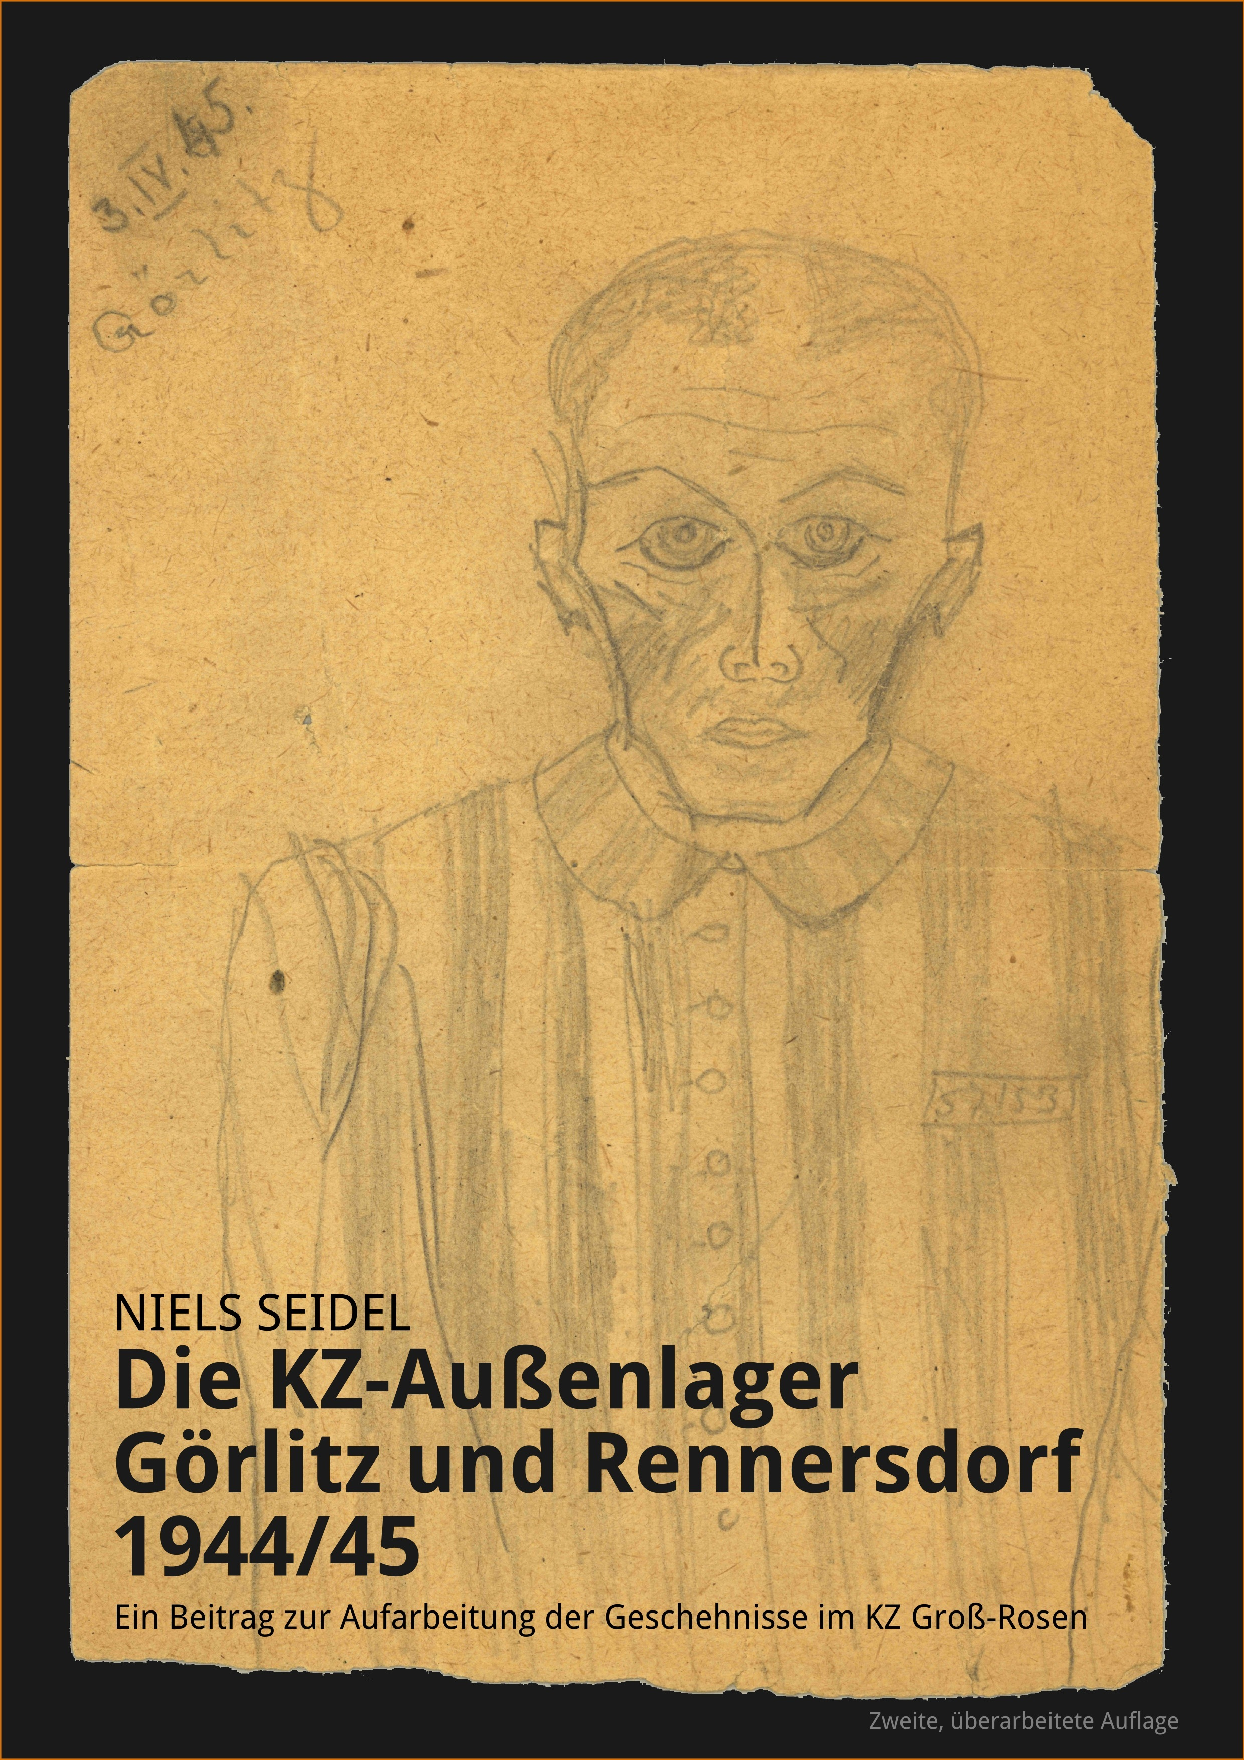
\includepdf{images/cover.pdf}
\newpage ~\newpage



\noindent{\Large{Die KZ-Außenlager Görlitz und Rennersdorf}}

\newpage
\normalsize

\begin{titlepage}
	\title{Die KZ-Außenlager\\ Görlitz und Rennersdorf\vspace{10 pt}
	\\\large{Ein Beitrag zur Aufarbeitung der Geschehnisse\\ im Konzentrationslager Groß-Rosen}}
	\author{Niels Seidel}
  \maketitle
\end{titlepage}


\small{
Herausgeber: Umweltbibliothek Großhennersdorf e.V.\\
www.umweltbibliothek.org | mail@umweltbiblithek.org
\\ \\
\textbf{Die KZ-Außenlager Görlitz und Rennersdorf}\\
Ein Beitrag zur Aufarbeitung der Geschehnisse\\ im Konzentrationslager Groß-Rosen
\\ \\
Autor: Niels Seidel\\
\href{http://www.nise81.com}{www.nise81.com} | \href{mailto:niels.seidel@nise81.com}{niels.seidel@nise81.com}\\
Version: 2.0\\
Datum: \today\\

\vspace{2.5cm}


Diese Publikation ist unter \emph{Creative Commons -- Namensnennung-NichtKommerziell-KeineBearbeitung 3.0 Deutschland} lizenziert und darf als Ganzes oder ausschnittweise vervielfältigt, verbreitet und öffentlich zugänglich gemacht werden, sofern dies im Text nicht anders vermerkt ist.\newline\vspace{10pt}

\includegraphics[height=20mm]{images/logo_cc.pdf}
\\ \\ \\


Die 1. Auflage erschien im Neisse Verlag, Dresden 2008\\
ISBN 978-3-940310-19-4\\
www.neiseverlag.de | mail@neisseverlag.de\\ \\

Lektorat: Luise Träger\\
Gestaltung und Satz: Niels Seidel / \LaTeX\\
Titelbild: Selbstportrait von Ben Mącznik aus dem Privatbesitz seines Sohnes Samson Munn.\\ \\


}
\normalsize
\newpage
\pagestyle{plain}
\setcounter{page}{5}
\tableofcontents
\newpage



\section*{Vorwort}
\addcontentsline{toc}{section}{Vorwort}Es war im Frühjahr 1994, als der inzwischen verstorbene Altbernsdorfer Ortschronist Siegfried Hittig uns Schüler anlässlich der Projekttage am Herrnhuter Gymnasium von einem Zug jüdischer Häftlinge erzählte, der sich zu Kriegsende, von Bernstadt kommend, am Fuße des Eichler-Berges in Rennersdorf verlor und schier spurlos verschwand. 
Niemand konnte mir eine Antwort darauf geben, was sich in diesem kleinen Dorf unweit der heutigen Grenzen zu Polen und der Tschechischen Republik im Winter 1945 abspielte. Weder meine Lehrer, noch meine um Rennersdorf ansässige Verwandtschaft hatten die leiseste Ahnung davon, was die Schülerin Katja Junge in einer Hausarbeit über das KZ Biesnitzer Grund fast 10 Jahre später zur Sprache brachte. Das Ausmaß und allein schon die Existenz nationalsozialistischer Konzentrationslager jenseits von Auschwitz und Buchenwald, sondern in der Oberlausitz, machten mich betroffen und neugierig zugleich. Rennersdorf war kein Einzelfall. Orte wie Bautzen, Großkoschen, Guben, Kamenz, Klein-Radisch, Niesky, Kunnerwitz, Niederoderwitz, Spohla, Weißwasser und Zittau reihen sich auf deutscher Seite ebenso in die Liste der ehemaliger Außenlager des KZ Groß-Rosen ein, wie das KZ-Außenlager in Görlitz, dessen Häftlinge sich 1945 auf einen Todesmarsch in das dafür gebildete Lager nach Rennersdorf begaben. Katja Junges Arbeit und die bis dato einzigen wissenschaftlichen Publikationen von Roland Otto bzw. Gräfe und Töpfer, in denen die KZ-Außenlager Görlitz und Rennersdorf ausführlicher Erwähnung fanden, ließen viele Fragen unbeantwortet und eröffneten lediglich die Auseinandersetzung mit einer Vielzahl von Aspekten. Dieses Versäumnis ist nicht den Autoren vorzuwerfen, sondern der Tatsache geschuldet, dass vorhandene Quellen bis 1990 gar nicht oder nur schwierig zugänglich waren. Beispielsweise hielt das Ministerium für Staatssicherheit sämtliche Prozessakten der Gerichtsverfahren gegen beteiligte NS-Verbrecher unter Verschluss, so dass selbige Dokumente noch heute nur mit erheblichen Auflagen eingesehen werden können. Darüber hinaus war es Historikern in der DDR nicht möglich, uneingeschränkt ausländische Archive zu kontaktieren und Informationen zu erbitten, geschweige denn, Zeitzeugen im westlichen Ausland zu besuchen. Roland Otto hatte noch dazu erhebliche Probleme, seine Diplomarbeit über die Verfolgung der Juden in Görlitz durchzusetzen, da er den so genannten Antifaschisten nicht die von ihnen allein beanspruchte Opferrolle zubilligte. Abgesehen von den damaligen politischen Blockaden war es vor dem Zeitalter des Internets schwierig, Personen, Orte und verschiedene Medien ausfindig zu machen oder in einem Zuge alle Jüdischen Gemeinden in Nordamerika auf der Suche nach Überlebenden zu kontaktieren. 

Anliegen dieses Buches ist es, die Gräuel des NS-Terrors jenseits von Buchwald und Auschwitz anhand der Erscheinung der KZ-Außenlager Görlitz und Rennersdorf exemplarisch zu vergegenwärtigen. Wer etwas über den Holocaust erfahren will, braucht nicht unbedingt in eine der bekannten KZ-Gedenkstätten fahren, wenn sich dutzende stille und unscheinbare Erinnerungs- und Gedenkorte in unmittelbarer Nachbarschaft befinden. Die in diesem Werk dokumentierten Geschehnisse leisten einen Beitrag für eine regionale und öffentliche Auseinandersetzung mit den zurückliegenden Diktaturen im Sinne einer zeitgemäßen Erinnerungsarbeit. Nicht zuletzt, um fremdenfeindlichen Tendenzen in der Oberlausitz entgegenzuwirken und den europäischen Dialog zu fördern.

\section*{Vorwort zur zweiten Auflage}
\addcontentsline{toc}{section}{Vorwort zur zweiten Auflage}Für die Herausgabe einer zweiten Auflage habe ich zwei Gründe. Erstens waren die 500 Exemplare der ersten Auflage im Neisse Verlag innerhalb von neun Monaten beim Verlag vergriffen und zweitens erlangte ich durch Leserbriefe, Rezensionen und nicht zuletzt durch die Auszeichnung mit dem Sächsischen Landespreis für Heimatforschung (Jugendpreis) vielfache Hinweise, das bestehende Werke zu verbessern und gewisse Abschnitte zu vertiefen.
Um die Verfügbarkeit künftig länger aufrecht zu erhalten, habe ich mich bewusst für eine digitale Publikation unter der freien Lizenz von \emph{Creative Commons} entschieden. Neue Erkenntnisse finden somit schneller zum Leser. 
Eine Übersicht über die Änderungen dieser Version sind im \emph{changelog}\footnote{\url{http://softbook.nise81.com/changelog.txt}.} verzeichnet. 

\section*{Einleitung}
\addcontentsline{toc}{section}{Einleitung}Ein Konzentrationslager war ursprünglich gleichbedeutend mit einem Gefangen- oder Internierungslager, in den Gruppen von Menschen festgehalten und konzentriert wurden. 
Zunächst betraf dies insbesondere Frauen und Kinder, die man angeblich aus Schutz vor Kampfhandlungen in solchen Lagern verwahrte. In Wahrheit diente die Gefangennahme als politisches Druckmittel, wie etwa im amerikanisch-spanischen Krieg oder dem Burenkrieg. Zumal diese Lager jeweils nur als vorübergehende Maßnahme gedacht waren, entsprachen sie in ihrem Wesen nicht dem systematischen Terror der nationalsozialistischen oder sowjetischen Lager\footnote{Vgl. Kotek / Rigoulot: Das Jahrhundert der Lager, S. 71.}. Gänzlich unabhängig von Kriegshandlungen wurde erstmals in Deutsch-Südwestafrika (heute Namibia) der Versuch unternommen Menschen in Konzentrationslagern zu internieren und durch Zwangsarbeit in so genannten Konzentrationslagern zu Grunde zu richten\footnote{Kotleg und Rigoulot schreiben, dass 1905 in den Konzentrationslagern mehr als die Hälfte (7862 Personen) der 10.632 Frauen und Kinder und 4137 Männer ums Leben kamen. Vgl. Kotek / Rigoulot: Das Jahrhundert der Lager, S.80.}. Der vorangegangene Versuch das Volk der Hereros vollkommen auszulöschen wurde durch Kaiser Wilhelm II\index{p}{Wilhelm II} aufgrund von Medienprotesten und wirtschaftlichen Belangen zwar abgebrochen, doch ebenso rassistisch und brutal durch Sklavenarbeit in Eisenbahnprojekten, sowie in privaten Wirtschaftsunternehmen fortgesetzt\footnote{Großen Privatunternehmen hatte man bereits eigene Lager zugesprochen, wohingegen kleine Firmen täglich die von ihnen benötigen Arbeitskräfte bezogen. Ebenda, S. 80ff. Vielfach unbekannt ist darüber hinaus, dass an den Gefangenen bereits medizinische Experimente durchgeführt wurden; u.a. von den späteren Lehrmeistern Josef Mengeles\index{p}{Mengele, Josef}, Eugen Fischer\index{p}{Fischer, Eugen} und Theodor Millisson\index{p}{Millisson, Theodor}.}.



Noch vor den Nationalsozialisten etablierte die Sowjetunion ein riesiges, dauerhaftes Lagersystem als administrative Maßnahme zur Isolation, Bestrafung und Versklavung politischer oder krimineller Delinquenten bzw. unschuldiger Menschen. Bereits im Jahre 1923 entwickelte die Lagerleitung auf den Solowezki-Inseln\index{o}{Solowezki-Inseln} am Weißrussischen Meer, ähnlich wie später in deutschen Konzentrationslagern, ein System der teilweisen Selbstverwaltung durch politische Häftlinge. Zu dem wurde ein Normensystem zur Maximierung der Arbeitsleistung geschaffen, dass sprichwörtlich die Vernichtung von Leben innerhalb der ersten drei Monate zum Ziel hatte\footnote{Naftaly Aronovich Frenkel\index{p}{Frenkel, Naftaly Aronovich}, ein zum Lagerkommandanten aufgestiegener Häftling prägte den Satz: \glqq Aus dem Häftling müssen wir alles in den ersten drei Monaten herausholen - danach brauchen wir ihn nicht mehr.\grqq~ Kotek / Rigoulot: Das Jahrhundert der Lager, S. 181.}. Im Hinblick auf  Organisation, wirtschaftliche Erwägungen und Massenmord gibt es weiterreichende Parallelen, aber natürlich auch Unterschiede zum System der nationalsozialistischen Konzentrationslager, auf die hier jedoch nicht weiter eingegangen werden soll.

Als Mittel staatspolizeilicher Gewalt fungierten die Konzentrationslager während der gesamten 12-jährigen Herrschaft der Nationalsozialisten. Formal legitimiert durch die \glqq Verordnung des Reichspräsidenten zum Schutz von Volk und Staate\grqq~wurden \glqq Beschränkungen der persönlichen Freiheit [...] außerhalb der sonst hierfür bestimmten gesetzlichen Grenzen [...]\grqq\footnote{RGB 1933, Teil 1, S83.} zur gängigen Praxis, um Personen für unbestimmte Zeit und ohne richterliche Verfügung in sogenannte Schutzhaft zu nehmen. Schutzhaft hatte den Charakter einer staatspolizeilichen Repressionsmaßnahme und diente durchaus nicht, wie es der Name vermuten läßt, dem Schutz der betreffenden Person.
\\
Die Entwicklung der Konzentrationslager einschließlich der Schutzhaft wurde durch die jeweilige außenpolitische Situation geprägt und lässt sich in vier Phasen einteilen. Während der Jahre 1933--1935 spricht man von der ersten Phase, in der die Schutzhaft als Instrument der Herrschaftssicherung diente. Die Isolation führender Oppositioneller brachte den Widerstand gegen die Nationalsozialisten zum Erliegen und sorgte für eine \glqq soziale Formierung\grqq~der Gesellschaft. Es entstanden eine Reihe von kleinen Konzentrationslagern, wie zum Beispiel in Niesky, Weißwasser, Leschwitz (heute: Weinhübel bei Görlitz) und Hainewalde, von denen nach einer straffen Neuorganisation im Jahr 1935 lediglich die Lager in Bad Sulza, Berlin-Tempelhof, Dachau, Hainewalde, Hamburg-Fuhlsbüttel, Kislau, Lichtenburg, Mohringen und Sachsenburg bestehen blieben.
In der zweiten Phase zwischen 1936 und 1938 waren jene Menschen von der Schutzhaft betroffen, die nicht dem nationalsozialistischen Bild entsprachen. In der damaligen Redeweise galt dies für Bibelforscher (Zeugen Jehovas), Assoziale, Berufs- und Gewohnheitsverbrecher, Arbeitsscheue, Homosexuelle und seit 1938, besonders im Gefolge der Reichsprogromnacht, auch für Juden und andere \glqq Nichtarier\grqq.
Kurz vor Kriegsbeginn setzte die dritte Phase ein. Der erwartete Anstieg der Gefangenenzahlen durch die Deportation von Juden in den besetzten Gebieten führte zu einer abermaligen Neuorganisation der Konzentrationslager. Zu den insgesamt sechs großen Lagern innerhalb des Reichsgebiets, die jeweils für mehrere tausend Gefangene ausgelegt waren, kamen nach Beginn des Krieges die Lager Auschwitz (1940), Hinzert (1940), Groß~Rosen (1941), Natzweiler (1941), Lublin (1941), Wewelsburg (1941), Arbeitsdorf (1942) und Stutthof (1942) hinzu. 
\\
Als im Winter 1941/42 die \glqq Blitzkrieg-Strategie\grqq~gegen die Sowjetunion scheiterte und eine Reihe von Niederlagen seitens der Nationalsozialisten folgte, musste man sich auf einen länger anhaltenden Abnutzungskrieg einstellen. Die kriegswirtschaftliche Umstellung auf den \glqq totalen Krieg\grqq~und die damit verbundene Mobilmachung von Arbeitskräften bestimmte maßgeblich die vierte Phase der Konzentrationslager, deren Auswirkungen hier am Beispiel der Lager in Görlitz und Rennersdorf dokumentiert werden. 
Beide Lager vermitteln exemplarisch Einblick in das Wesen der nationalsozialistischen Gewaltherrschaft, die nicht als zentrales Ungeheuer, sondern als allgegenwärtige Erscheinung, fernab von Auschwitz und Buchenwald auftrat. Die Ansiedlung von Konzentrationslagern in der unmittelbaren Nähe von Rüstungsbetrieben konfrontierte die alltägliche Lebenswelt der Deutschen mit den Ausprägungen von Terror und Gewalt im Leben der KZ-Häftlinge. Die Wechselwirkungen und Beziehungen zwischen KZ-Kosmos und zivilem Alltag, Einfluss und Zusammenspiel von Wirtschaft und Staat, sowie Wissen und Bewusstsein der Bevölkerung sind am Gegenstand der KZ-Außenlager besser zu erklären als an anderen Erscheinungsformen der nationalsozialistischen Herrschaft. Anliegen dieser Dokumentation ist die rationale Darstellung der Geschehnisse und Zusammenhänge in den KZ-Außenlagern Görlitz und Rennersdorf einschließlich ihrer Auswirkungen in der Nachkriegszeit. Anstatt einzelne Gruppen als Schuldige auszumachen, wird versucht das Wirken des Systems als Ganzes beleuchtet.

 
\chapter{Das KZ-Außenlager Görlitz}

Die ersten jüdischen Zwangsarbeiter verschleppte man noch vor der Entstehung des KZ-Außen\-lagers\index{p}{Rechenberg, Erich} in das Barackenlager im Biesnitzer Grund; damals im Rahmen der Organisation Schmelt. Zuvor waren am selben Ort bereits Kriegsgefangene inhaftiert. Alle drei Lagertypen entstanden auf Veranlassung der Waggon- und Maschinenbau AG (WUMAG) Görlitz, welche das Lager errichten ließ und dessen unfreiwillige Bewohner im Sinne der nationalsozialistischen Ideologie für die Kriegsproduktion ausbeutete. Verantwortungslos und zynisch bezeichnete das Unternehmen diese Haftstätten als \glqq Menschenlager\grqq\footnote{In einem Geschäftsbericht der WUMAG vom 15.03.1944 heißt es: \glqq Durch die Errichtung der Barackenstadt, die Sie uns in der Sitzung vom 11. November 1943 genehmigt hatten, wird ein Teil der anderen Menschenlager frei werden.\grqq, StArchD 11693 WUMAG / 1258.}, deren Bestände möglichst erschöpfend und gewinnbringend für den Arbeitseinsatz genutzt wurden. \newline
Als das Lager im Sommer 1944 dem KZ Groß-Rosen\index{o}{Groß-Rosen} unterstellt wurde und folglich die SS die Verantwortung für die Beschaffung und Disziplinierung der Häftlinge übernahm, rückte eine Gesellschaft von zunehmend erschöpften, innerlich gebrochenen und apathischen Wesen ins Auge der Görlitzer Öffentlichkeit. Es handelte sich um eine Gruppe von 1500 Juden -- um Männer und Frauen, die sich hinsichtlich ihres Alters, ihrer Nationalität und ihrer einstigen gesellschaftlichen Stellung wesentlich unterschieden, jedoch dem System und dem Terror des Konzentrationslagers, wenn überhaupt, nur schwerlich Stand halten konnten. Bedingt durch mangelnde medizinische Versorgung, widerliche hygienische Verhältnisse, schlechte Kleidung und unzureichende Ernährung häuften sich Krankheiten und Todesfälle. Auch die harte und unmenschliche Arbeit in den Werken der WUMAG trug wesentlich zur Sterblichkeit der Häftlinge bei.
\\
\section{Zur Vorgeschichte}
Im Südwesten von Görlitz, unmittelbar an der Grenze zur kleinen Gemeinde Biesnitz, die erst 1951 in die Stadt Görlitz eingemeindet wurde, errichtete die WUMAG auf dem Gelände einer alten Ziegelei\footnote{Die Ziegelei war ehemals Teil der Maschinenfabrik Roscher, in welcher die damals bekannten Maro Ziegeleimaschinen hergestellt wurden. Laut einer Flurstückskarte aus dem Jahr 1935 befand sich die Ziegelei und damit auch das spätere Lager auf Görlitzer Flur.} ein Barackenlager mit der Absicht, dort Zwangsarbeiter einzuquartieren. Das Grundstück ist bis heute städtisches Eigentum\footnote{Grundbuchblatt 14286 Görlitz: Flurstück 38/15, Amtsgericht Görlitz.}, wurde jedoch vor dem Krieg an den Fabrikanten Roscher\index{p}{Roscher} und einen Bauern namens Ecke\index{p}{Ecke, Erich} verpachtet.
Im Jahre 1939 kündigte die Stadt alle Pachtverträge\footnote{Erich Ecke konnte ab dem Jahre 1939 die Wiese im Biesnitzer Grund nicht mehr nutzen. Laut Aussage von Alfred Ecke, dem Sohn des Bauern.} zugunsten der WUMAG, welche bereits anderenorts Barackenlager errichtet hatte\footnote{Erste Erkundigungen über Barackenfabrikationen und deren Preisbindung erfolgten am 16.10.1939. Am 24.10.1939 tritt man in Verhandlungen mit dem Reichsarbeitsdienst wegen Übernahme von Baracken und erteilt einen Auftrag für 20 Stück. StArchD 11693, 1258 (Bild-Chronik III).}. Die Kosten und die Verantwortung für diese Bauprojekte trug die WUMAG allein\footnote{In der Bilanz 1940/41 ist der Kauf von fünf Baracken für das Russenlager mit 43.000 RM verbucht. StArchD 11693 / 1027 und 1258 (Bild-Chronik III).}. Im Biesnitzer Grund führte man zunächst ein Lager für 300 französische Kriegsgefangene\footnote{StArchD 11693 WUMAG / 1035 1164: Meldung der WUMAG-Lager an die Rüstungsinspektion VIIIa Breslau: WUMAG-Liste über gemietete Räumlichkeiten.}.
Nach dem Russlandfeldzug entstand ein zweites Lager in unmittelbarer Nachbarschaft für 450 sogenannte \glqq Ostarbeiter\grqq\footnote{Ebenda. Vgl. auch Thomas Warkus: Kriegsgefangene und Fremdarbeiter im nationalsozialistischen Deutschland 1939--1945. Das Beispiel Görlitz. Ostarbeiter ist seit dem 2. Februar 1942 die amtliche Bezeichnung für sowjetische Fremdarbeiter und Fremdarbeiterinnen. Vgl. Martin Weinmann: Das Nationalsozialistische Lagersystem, S. LIX.}. Dergleichen galten als slawische Untermenschen, für die die nationalsozialistische Rassenlehre, genauso wie für die Juden, allenfalls ein Dasein als Staatssklaven vorsah\footnote{Wolfgang Sofsky: Die Ordnung des Terrors -- Das Konzentrationslager, S. 139f.}. Über ihr Schicksal ist in Görlitz allerdings nur wenig bekannt.
\newline
Im Geschäftsbericht der WUMAG vom November 1943 beklagt sich die Geschäftsführung über die hohen Kosten, die die vom Arbeitsamt zugewiesenen Zwangsarbeiter verursachten. Nicht nur über den Aufwand die ungelernten Arbeitskräfte anzulernen wird geklagt, sondern auch über Belastung für Unterbringung, Verpflegung, Überwachung, Errichtung einer Entlausungsstation und einer Sanitätsstube. Weiter heißt es: \glqq Im Gegensatz zu den Franzosen sind wir mit den russischen Kriegsgefangenen in Bezug auf ihren Arbeitswillen und ihr Verhalten sehr zufrieden. Leider können sie wegen ihres Gesundheitszustandes im Durchschnitt aber nur als 50 Prozent leistungsfähige Kräfte eingesetzt werden.\grqq\footnote{StArchD 11693 / 1027.}. Anstatt sich der Ursachen anzunehmen, setzte man auf gewaltsame Mittel, um eine ökonomisch rationale Kostenminimierung zu erreichen.
Bereits am 2. August 1942 kam es im \glqq Russenlager\grqq~zu einer Arbeitsverweigerung wegen schlechter Kost. Unter Androhung von Erschießung gaben die extra angerückten Soldaten den Streikenden zwei Minuten Bedenkzeit, um wieder an die Arbeit zu gehen. Sie gaben nach, doch drohte man mit sofortiger Hinrichtung, sollte sich solch ein Vorfall wiederholen\footnote{StArchD 11693 / 1258 Bild-Chronik III. Vgl. auch: Thomas Warkus: Kriegsgefangene und Fremdarbeiter im nationalsozialistischen Deutschland 1939--1945. Das Beispiel Görlitz.}.

\subsection{Das Zentrale Arbeitslager der Organisation Schmelt}
Der SS-Oberführer und Breslauer\index{o}{Breslau} Polizeipräsident Albrecht Schmelt\index{p}{Schmelt, Albrecht} koordinierte in seiner Position als \glqq Sonderbeauftragter des Reichsführers der SS für fremdvölkischen Arbeitseinsatz in Oberschlesien\grqq, seit 1940 die Zwangsarbeit in Ghettos und Arbeitslagern. Die nach ihm benannte Organisation operierte anfangs nur in Oberschlesien weitete sich jedoch schon bald nach Niederschlesien und ins Sudetenland aus. Es entstanden so genannte Zentrale Arbeitslager (ZAL) in der Nähe von kriegswichtigen Unternehmen wie der WUMAG Görlitz\footnote{Bei einer Wirtschaftsprüfung vom 29. Oktober bis 9. November 1940 wurde die WUMAG zum kriegswichtigen Unternehmen erklärt. StArchD 11693 / 1258 Bild-Chronik III. Das ZAL Görlitz wird in Zusammenhang mit dem Rüstungsbetrieb WUMAG genannt. Vgl. Alfred Konieczny: Die Zwangsarbeit der Juden in Schlesien im Rahmen der Organisation Schmelt, S. 104.}, in denen zumeist die jüdische Bevölkerung Oberschlesiens Zwangsarbeit verrichtete\footnote{Vgl. Martin Weinmann: Das Nationalsozialistische Lagersystem, S. LVIII.}. \glqq Die organisatorische Umsetzung des Zwangsarbeitereinsatzes oblag den Jüdischen Ältestenräten in Oberschlesien, die auf deutsche Verordnung in Sosnowiec zusammengefasst waren [...]\grqq, schreibt Andrea Rudorff\footnote{Andrea Rudorff: Das Lagersystem der Organisation Schmelt in Oberschlesien. S. 159.}. Die Verteilung jüdischer Arbeitskräfte richtete sich nach den Bedarfsmeldungen der Betriebe, anhand derer der Jüdische Ältestenrat der Organisation Schmelt schriftliche Aufforderungen zum Arbeitseinsatz versandt. Die Verteilung jüdischer Arbeitskräfte beruhte auf einer zwischen Schmelt und den jeweiligen Betrieben getroffenen Vereinbarung, die im Sinne strikter Aufwandsminimierung die Löhne und die innere Organisation der Arbeitslager festlegte\footnote{Vgl. Israel Gutman: Enzyklopädie des Holocaust -- Band 2, S. 1070.}. Schmelts\index{p}{Schmelt, Albrecht} Lagerführung stützte sich auf eine Häftlingsselbstverwaltung, die sich bereits in Konzentrationslagern bewährte hatte, und sparte somit an Wachpersonal. Es gab einen Ältesten, einen Krankenbehandler und einen Stenotypisten für je 150 Zwangsarbeiter, genauso wie einen Schuster, einen Schneider und einen Koch samt Küchengehilfen\footnote{Vgl. Martin Weinmann: Das nationalsozialistische Lagersystem (CCP), S. LVIII. Vgl. Alfred Konieczny: Die Zwangsarbeit der Juden in Schlesien im Rahmen der Organisation Schmelt, S. 101.}. Somit genügte ein Wachmann bzw. Hilfspolizist oder Angehöriger des Werkschutzes zur Bewachung von je 40 Gefangenen.
\newline
Der bisherige Erkenntnisstand über das Lagersystem der Organisation Schmelt insgesamt sowie über das ZAL Görlitz im Speziellen ist äußerst unzureichend und beschränkt sich auf wenige Quellen\footnote{Vgl. Andrea Rudorff: Das Lagersystem der Organisation Schmelt in Oberschlesien. S. 159.}.
Das Lager der Organisation Schmelt in Görlitz entstand wahrscheinlich am 26. April 1943\footnote{Entsprechend einer Notiz in der \glqq Chronik zur Geschichte des antifaschistischen Widerstandskampfes\grqq. Nathan Klajman\index{p}{Klajman, Nathan} gibt an, im Mai desselben Jahres in das Lager gekommen zu sein. ZHI 301/2765.} im Biesnitzer Grund. Hinweise, wonach im April 1943 die Häftlinge des ZAL Görlitz nach Kittliztreben (Trzebień, Polen)\index{o}{Kittliztreben} überstellt wurden\footnote{Martin Weinmann: Das nationalsozialistische Lagersystem (CCP), S. 579.} konnten ebenso wenig bestätigt werden wie die Existenz eines \glqq Judenlagers\grqq~innerhalb des Maschinenbaukomplexes der WUMAG (siehe Luftaufnahme S.~\pageref{maschinenbaufoto})\footnote{Nach Ermittlungen von Kurt Wolf aus Löbau, der mir seine Erkenntnisse im Zusammenhang mit dem Schmelt-Lager und dem Außenlager Görlitz zuteil werden ließ.}.
Zeitzeugenberichte aus dem Biesnitzer Lager sind äußerst rar. Die Familie Ecke des benachbarten Bauernhofes hatte während dieser Zeit jedenfalls Zugang zum Lager, um dort die Jauche aus der Latrine abzuschöpfen. Der Bauer Ecke\index{p}{Ecke, Erich} pflegte sogar eine persönliche Beziehung zu einem der Insassen\footnote{Es kam während dessen zu Tauschgeschäften (Leder und Stoffe) zwischen Eckes und dem Gefangenen. Nach der Befreiung des Lagers kam es zu einem Wiedersehen auf dem Hof der Eckes. Laut Aussage von Alfred Ecke.}.~\newline
Der Schmelt-Häftling Nathan Klajman\index{p}{Klajman, Nathan}:
\begin{leftbar}
Im Mai 1943 wurde ich zusammen mit 70 Leuten ins Konzentrationslager nach Görlitz verschleppt. Dort waren 200 Juden. Wir arbeiteten in der Munitionsfabrik, wir wurden unbarmherzig geschlagen. Der Judenälteste Babinger\index{p}{Babinger} war zu uns sehr gut.
Ich blieb dort 10 Monate. Wir bekamen 40 dkg [= 400 Gramm] Brot und Suppe. Die Meister misshandelten uns.\footnote{Nathan Klajman ist in Berlin geboren und durchlebte eine ganze Reihe von Arbeitslagern, darunter Annaberg (auch \glqq Kretschamberg\grqq, heute Cha\l upki, Polen), Graditz (Oberschlesien), bevor er in das KZ-Außenlager Kittlitzstreben (Trzebień, Polen) gebracht wurde. Anfang Februar zwang man ihn und viele andere, einen Todesmarsch über Görlitz nach Zittau anzutreten. Zu Kriegsende befreite man ihn im KZ-Außenlager Zittau (heute: Sieniawka, Polen). ZIH 301/2765.}
\end{leftbar}
Der Schmelt-Häftling Jakob F.\index{p}{F., Jakob}:
\begin{leftbar}
Nach 5--6 Monaten wurde eine Gruppe von 50 Mann, darunter auch ich, [vom ZAL Neukirchen\index{o}{Neukirchen} bei Breslau\index{o}{Breslau}] nach Görlitz abtransportiert. [...] Görlitz war ein kleines Judenlager, ca. 300--350 Juden. Gearbeitet wurde bei der Firma WUMAG -- Waggon- und Maschinenbau -- ein großer Betrieb. [...] Ich mit noch acht Kameraden waren beschäftigt bei Dudel\index{p}{Dudel} als Schachtarbeiter und beim Bau großer Fabrikhallen. Kleidung: Zivil. [...] Bewachung: Wehrmacht. Bei der Arbeit bewacht durch Werkschutzleute des Betriebes Waggonbau. Judenältester: Benjamin R.\index{p}{R., Benjamin} [...] Judenfrauen: 12--13Frauen als Lagerpersonal. [...] Nach 2--3 Monaten wurden die Frauen abtransportiert, wohin weiß ich nicht. Anfang 1944 wurde Görlitz liquidiert und wir kamen ins KZ Kittlitztreben\index{o}{Kittlitztreben} [Trzebień, Polen].\footnote{Der Nachname des Zeugen wurde aus datenschutzrechtlichen Gründen vom Internationalen Suchdienst in Bad Arolsen nicht bekannt gegeben. ISD Sachdokumente M 9 Sakrau, S. 1 (2006).}
\end{leftbar}

\glqq Das Schicksal der jüdischen Gefangenen in den Lagern der Organisation Schmelt unterschied sich zum größten Teil nicht von dem aller anderen Insassen von Konzentrationslagern.\grqq, heißt es in der Enzyklopädie des Holocaust\footnote{Israel Gutman (Hrsg.): Enzyklopädie des Holocaust, Band 2, S. 1071.}.
\newline
Nathan Klajman\index{p}{Klajman, Nathan} gab an, zwischen Mai 1943 und März 1944 im ZAL Görlitz inhaftiert gewesen zu sein
\footnote{Nathan Klajman, ZIH 301/2765.}. Anhand der Belegschaftsstatistiken der WUMAG kann keine Belegung mit Schmelt-Häftlingen belegt werden. Offenbar wurden jene Zwangsarbeiter entgegen späterer Statistiken entsprechend ihrer Nationalität, statt vermeintlichen Religionszugehörigkeit verzeichnet\footnote{Zwischen Februar und März 1944 reduziert sich die Zahl der unter \glqq Sonstige\grqq~erfassten Ausländer um 85 Personen. Neben Belgiern, Franzosen, Polen und Russen erscheint die Zeile \glqq Sonstige\grqq~ab September 1944 mit dem handschriftlichen Vermerk \glqq Juden und Häftlinge\grqq. StArchD 11693 / 1258 (Bild-Chronik III).}.
\newline
Bereits Ende 1941 beschloss man im Zusammenhang mit der Endlösung der Judenfrage erstmals die Auflösung der ohnehin zeitlich befristeten ZAL. Die Umsetzung des Beschlusses verschob sich aufgrund erheblicher Einwände seitens der Wehrmacht und des Reichssicherheitshauptamtes, bis Himmler\index{p}{Himmler, Heinrich} 1943 die Auflösung der Lager, in denen die Arbeitskraft der Häftlinge als nicht kriegswichtig angesehen wurde, durchsetzte. Die WUMAG Görlitz befand sich in dieser Zeit in einer starken Abhängigkeit von ausländischen und jüdischen Fachkräften, um die von der Wehrmacht geforderten Rüstungsgüter liefern zu können\footnote{Vgl. Thomas Warkus: Kriegsgefangene und Fremdarbeiter im nationalsozialistischen Deutschland 1939--1945. Das Beispiel Görlitz.}. Es bestand also eine Notwendigkeit möglichst alle Arbeitskräfte zu behalten.
Unter der Führung von Adolf Eichmann\index{p}{Eichmann, Adolf} wurden 28 Lager in Niederschlesien und im Sudetenland -- nach vorheriger \glqq Selektion\grqq~der Häftlinge -- dem KZ Groß-Rosen\index{o}{Groß-Rosen} angegliedert, 20 davon als Außenlager\footnote{15 dieser Lager übergab man der Kommandantur von Auschwitz.}. Häftlinge aus über 125 Lagern wurden auf die Außenlager\footnote{Im folgenden soll nun von \glqq Außenlagern\grqq~oder \glqq Nebenlagern\grqq~gesprochen werden. Im SS-Sprachgebrauch hießen diese Lager im Falle von Männerlagern \glqq Arbeitslager\grqq~(abgekürzt AL) und bei Frauenlagern \glqq Frauenarbeitslager\grqq~(FAL), zum Teil auch \glqq Außenkommandos\grqq. Vgl. Isabell Sprenger: Groß-Rosen, S. 227.} von Groß-Rosen\index{o}{Groß-Rosen} und Auschwitz\index{o}{Auschwitz} verteilt\footnote{Vgl. Alfred Konieczny: Die Zwangsarbeit der Juden in Schlesien im Rahmen der Organisation Schmelt, S. 107.}. Das ZAL in Görlitz muss als eines der letzten Lager, spätestens Mitte 1944, von Groß-Rosen\index{o}{Groß-Rosen} übernommen worden sein.


\begin{flushleft}
    \setlength{\fboxsep}{0pt}
\begin{figure}
	\fbox{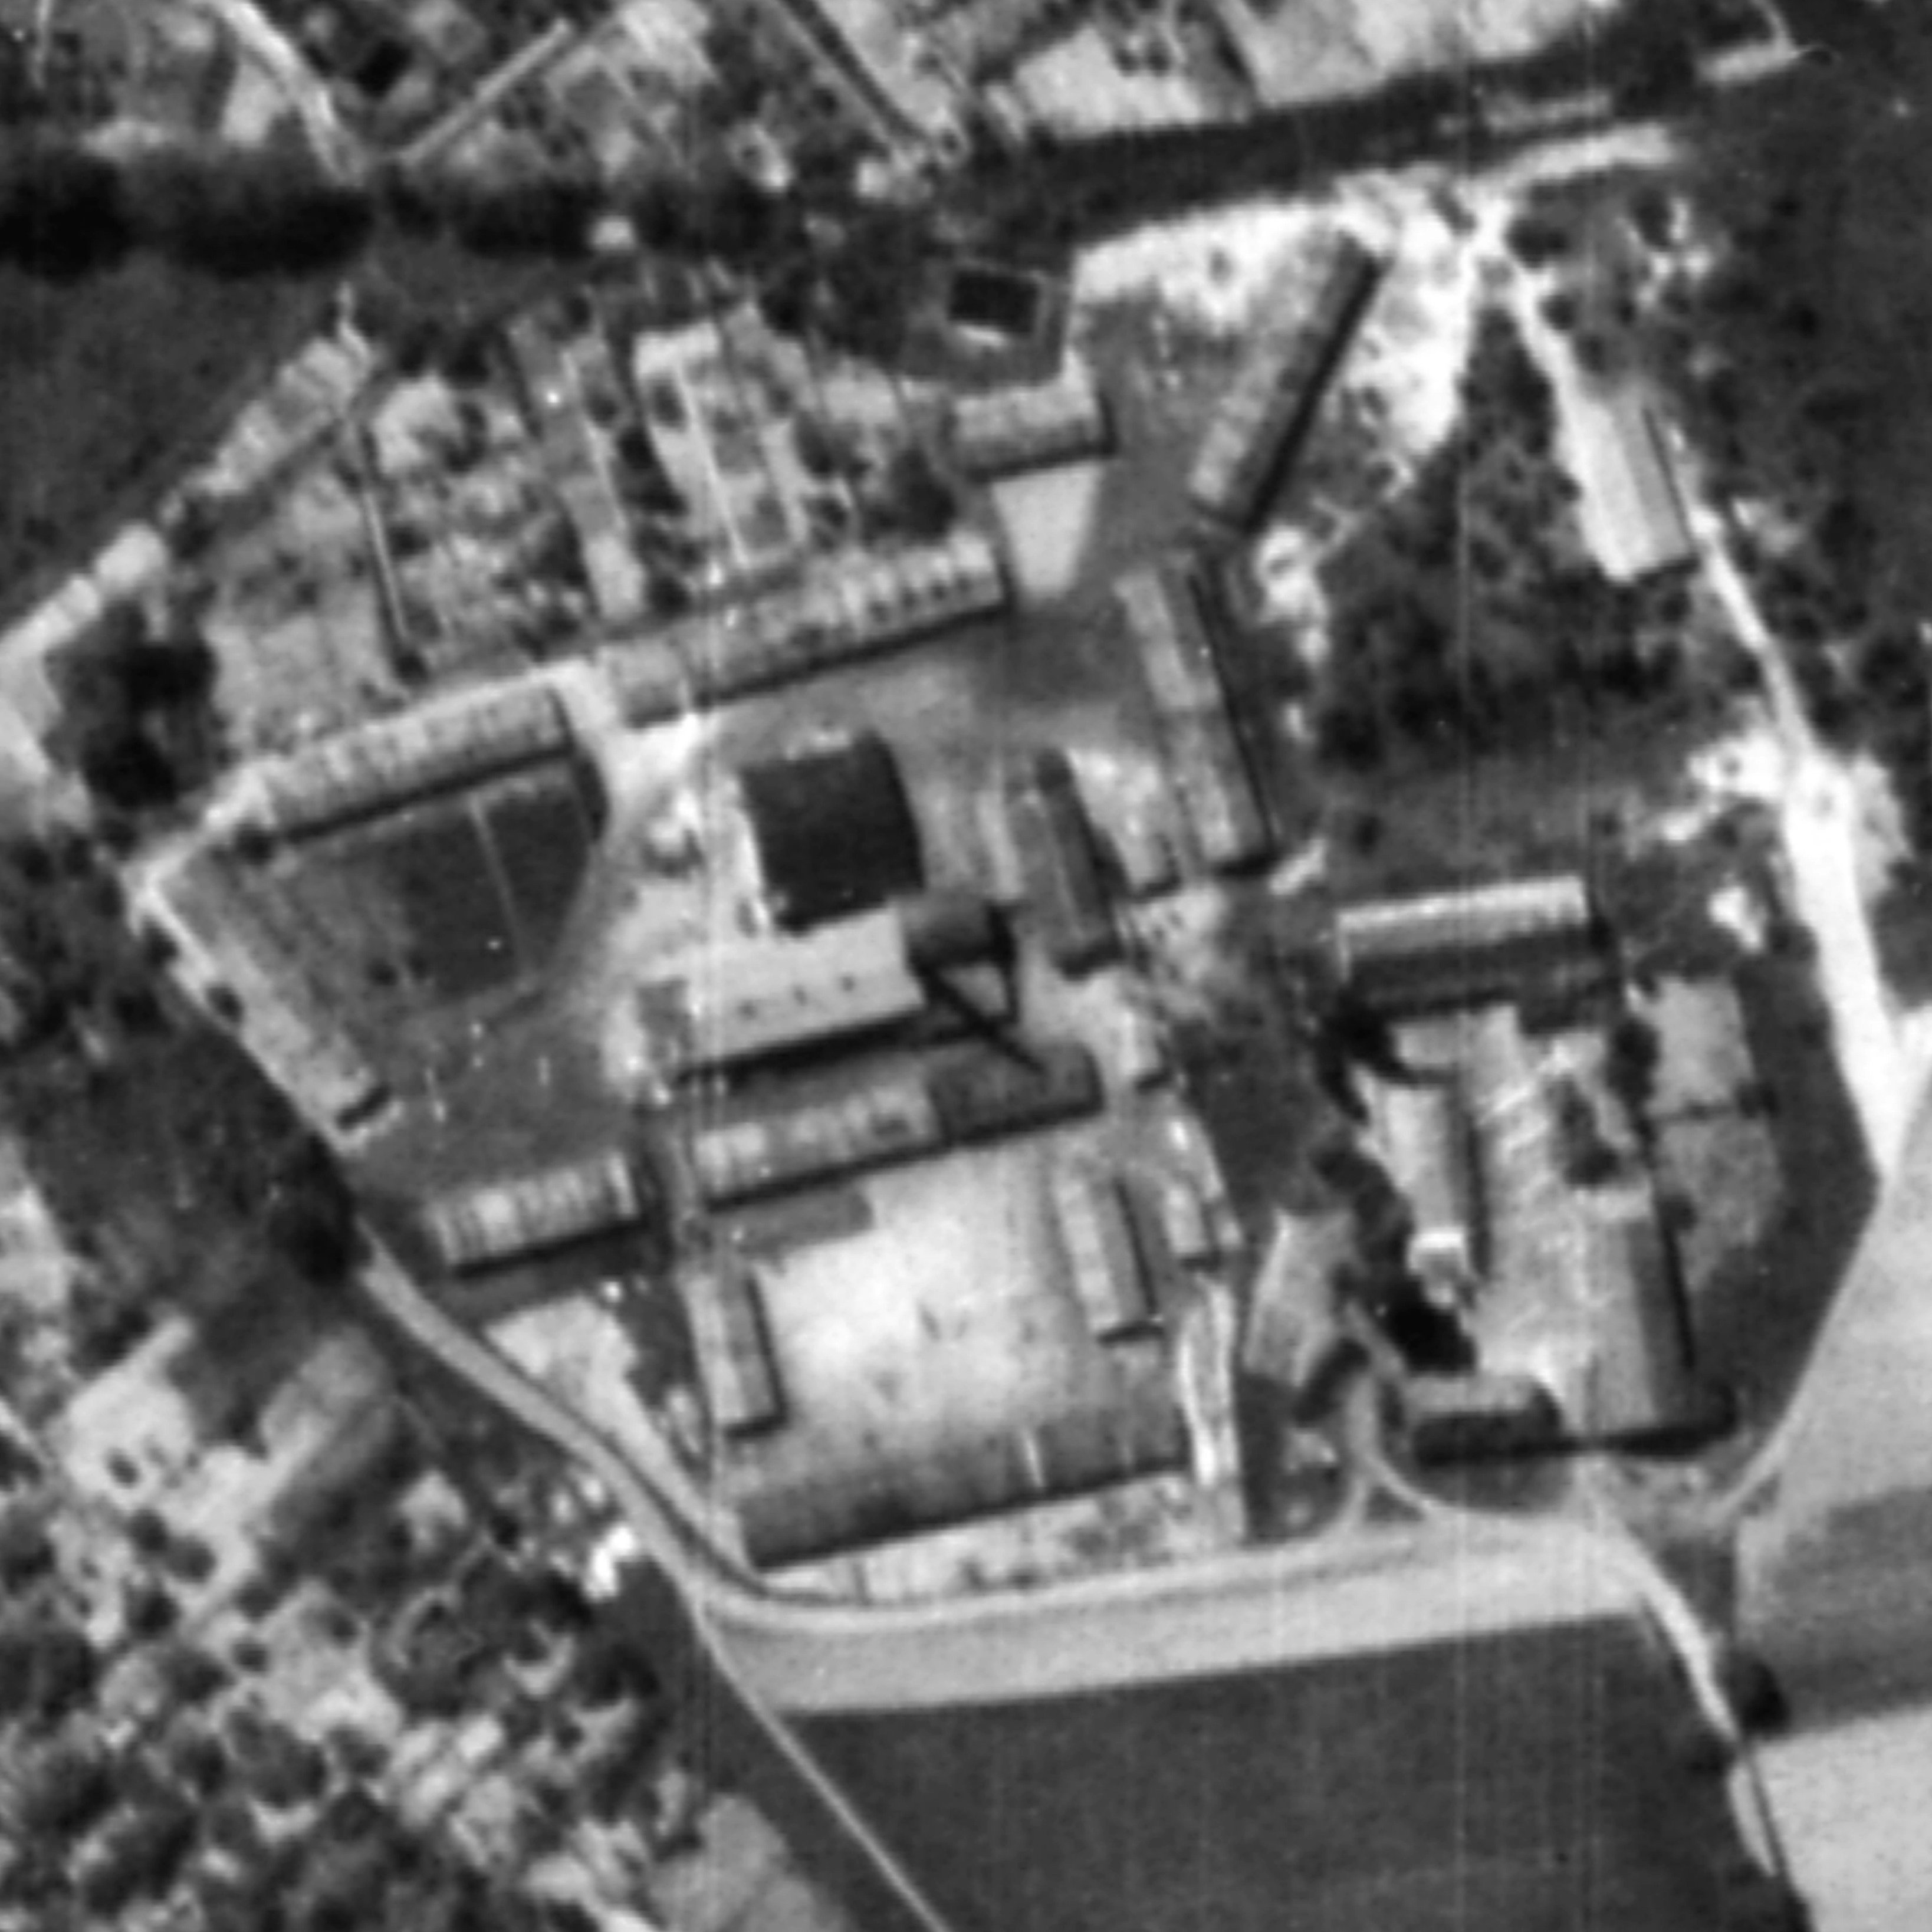
\includegraphics[width=.99\linewidth]{images/lager0.jpg}}
	\caption[Luftaufnahme des Lagers, 30. Mai 1945]{Luftaufnahme des Barackenlagers im Biesnitzer Grund vom 30. Mai 1944. Luftbilddatenbank, Ing.-Büro Dr. H.G. Carls.}
\end{figure}
\end{flushleft}

\myfigure[grossrosen0]{grossrosen0}{}{KZ Groß-Rosen}{KZ Groß-Rosen}{0}



\begin{fshaded}\vspace{-.5cm}\subsection*{Das Konzentrationslager Groß-Rosen\index{o}{Groß-Rosen}}
Etwa 60km südwestlich von Breslau in der heutigen Kreis Wa\l brzych befindet sich das Dorf Rogo\'znica, dessen deutscher Name Groß-Rosen\index{o}{Groß-Rosen}  während des Zweiten Weltkrieges eines der größten und berüchtigsten nationalsozialistischen Konzentrationslager bezeichnete. Die gute Eisenbahnanbindung an der Strecke von Jauer nach Striegau und insbesondere der nahe der Ortschaft gelegene Steinbruch mit seinem großen Vorkommen an schwarz-weißen Schlesischen Granits weckte bald schon das Interesse des SS-Unternehmens \glqq Deutsche Erd- und Steinwerke GmbH\grqq~\-(DEST). Im Jahre 1940 erwarb bzw. pachtete die DEST den Steinbruch und das Steinbruchgelände. Geplant war eine Vergrößerung des Steinbruchs und die rentable Herstellung von Werksteinen im Umfang von 50.000 Kubikmetern jährlich. Die zum Abbau benötigten Arbeitskräfte konnten aufgrund der bestehenden Zusammenarbeit mit der \emph{Inspektion der Konzentrationslager} im KZ Sachsenhausen in gleicher Weise durch den Einsatz von KZ-Häftlinge aufgebracht werden. In Groß-Rosen\index{o}{Groß-Rosen} wurde ein Außenkommando des KZ-Sachsenhausen errichtet. Am 2. August 1940 verlegte man die ersten 100 Gefangenen vom Hauptlager dorthin. Bereits 1941 beabsichtigte man eine Erweiterung des Steinbruchs auf 400\,m Länge, 140\,m Breite und 70--80\,m Tiefe. Die Zuführung von Arbeitskräften und Leitung des Lagers von Sachsenhausen aus, erwies sich zunehmend als schwierig, so dass Groß-Rosen\index{o}{Groß-Rosen} schlussendlich am 1. Mai 1941 in ein selbständiges Konzentrationslager umgewandelt wurde. Bis zum Januar 1945 stieg die Zahl der Inhaftierten von anfangs 900 auf 76728 an. Die alleinige Beschäftigung der Häftlinge im Steinbruch und im Granitwerk sowie in verschiedenen Kommandos innerhalb des Lagers (Maurer-, Tischler-, Schuster-, Gärtner- und Webereikommando) konnte aufgrund der steigenden Anforderungen der totalen Kriegsführung nicht aufrecht erhalten werden, so dass bereits 1942 das erste Außenlager in Breslau-Lissa (Wroc\l aw-Leśnica, Polen)\index{o}{Breslau-Lissa} eingerichtet wurde. Die meisten der ungefähr 100 Außenlager (siehe Karte~\mymapsref{grnebenlager}) entstanden bei bestehenden oder aus luftbedrohten Gebieten verlegten Betrieben der Kriegswirtschaft bzw. Rüstungsindustrie.
Eine gesonderte Stellung hatten die 12 Lager des Komplex Riese im Eulengebirge, in denen 13.000 jüdische Häftlinge unterirdische Fertigungsstätten und ein neues Führerhauptquartier bauten. Mit Herannahen der sowjetischen Truppen im Januar 1945 begann die schrittweise Evakuierung der bedrohten Außenlager, während das Hauptlager durch mehrere Kolonnen der von Auschwitz kommenden Todesmärsche maßlos überfüllt war. Um den 8./9. Februar 1945 erfolgte der Abtransport der Häftlinge aus Groß-Rosen\index{o}{Groß-Rosen} nach Buchenwald\index{o}{Buchenwald}, Flossenbürg\index{o}{Flossenbürg} (bzw. dessen Außenlager Hersbruck\index{o}{Hersbruck} und Leitmeritz\index{o}{Leitmeritz}), Mauthausen\index{o}{Mauthausen} und die Außenlager Dora\index{o}{Dora} und Nordhausen\index{o}{Nordhausen} des KZ Mittelbau. Nur wenige Häftlinge blieben in Groß-Rosen\index{o}{Groß-Rosen} zurück und wurden am 13. Februar 1945 von der sowjetischen Armee befreit.
\end{fshaded}

\mymapfigure[grnebenlager]{map_nebenlager300}{}{Außenlager des KZ Groß-Rosen}{Außenlager des KZ Groß-Rosen}{0}{}


\section{Entstehung des KZ-Außenlagers Görlitz}
Die Auflösung der großen Ghettos in Schlesien und des Generalgouvernements sowie die \glqq Säuberungsaktionen\grqq~in Transkarpathien und Ungarn bedingten, ebenso wie die Auflösung des KZ Plaszow\index{o}{Plaszow}, seit März 1944 die Errichtung zahlreicher Männer- und Frauenlager unter dem Kommando Groß-Rosens\index{o}{Groß-Rosen}\footnote{Vgl. Alfred Konieczny: Frauen im Konzentrationslager Groß-Rosen in den Jahren 1944-1945, S. 7. Vgl. auch: Israel Gutman: Enzyklopädie des Holocaust, Band 1, S. 570f.} (siehe Karte~\mymapsref{grnebenlager}). Die erste Erwähnung fand das Außenlager Görlitz am 09.06.1944 durch das Wirtschaftsverwaltungshauptamt der SS. Am 08. August 1944 übernahm SS-Oberscharführer Zunker\index{p}{Zunker, Winfried} in der Funktion des Lagerführers\index{p}{Zunker, Winfried}, zunächst das Lager für Männer. Ab September stand auch das neu gebildete Frauenlager unter seiner Leitung.\newline

Sowohl in der Literatur als auch im Volksmund wird das Barackenlager im Biesnitzer Grund, in dem unter anderem KZ-Häftlinge untergebracht waren, als \glqq KZ Biesnitzer Grund\grqq~\linebreak oder \glqq KZ Görlitz\grqq~bezeichnet.
Die Bezeichnung \glqq Biesnitzer Grund\grqq~ mag den Görlitzer Bürgern ein Begriff sein, doch ist der Name sowohl international als auch seitens der ehemaligen Gefangenen gänzlich unbekannt.\newline

Wenngleich die Wehrmacht oder später die SS an diesem Ort bestimmte Personengruppen \glqq konzentrierte\grqq, wurde es von amtlichen Stellen stets unter anderen Namen geführt. Zunächst als Außenlager des Stalag VIII A\footnote{Stammlager für Kriegsgefangene im Wehrbezirk VIII A (1. Lager im Wehrkreis VIII Breslau).}, als Arbeitslager der Organisation Schmelt, anschließend wahrscheinlich wieder als Außenlager des Stalag.
Erst durch die Übernahme des Lagers durch das KZ Groß-Rosen\index{o}{Groß-Rosen} galt es offiziell als Außenlager des KZ Groß-Rosen\index{o}{Groß-Rosen}, aber nicht als Konzentrationslager, da ausschließlich jene 25 Lager im definierten Sinne zu den Konzentrationslagern gehörten, die von der Inspektion der Konzentrationslager als solche geführt wurden\footnote{Diese Differenzierung ist für die Geschichtsschreibung vorteilhaft, um strukturelle Unterschiede und Verknüpfungen der Lager zu verdeutlichen. Im übrigen gelten auch die frühen Schutzhaftlager der Jahre 1933--1935, wie etwa jene in Leschwitz oder Hainewalde, nicht als Konzentrationslager. Verzeichnis der Konzentrationslager und ihrer Außenkommandos gemäß \textsection~42 Abs. 2 BEG, in Bundesgesetzblatt (1982), S. 1571--1579; Vgl. Gudrun Schwarz: Die nationalsozialistischen Lager.
An anderer Stelle ist von 30 Konzentrationslegern die Rede. Vgl. Karin Orth: Die Konzentrationslager-SS und die Shoah, S. 93 in Gerhard Paul (Hrsg.): Experten des Terrors.}. Dieser namentliche Unterschied soll jedoch nicht über den Terror und Vernichtungscharakter der Außenlager hinwegtäuschen.

\paragraph{Der Aufbau des Lagers} Das Lager war umgeben von vier Wachtürmen (siehe Bild~\mypicsref{wachturm}) und einem fünf Meter hohen, elektrisch geladenen Stracheldrahtzaun\footnote{Aussage von Bendet Perle (Michal Zylberberg). LArchB B Rep 058 Bd. 3.} inklusive teilweisem Sichtschutz. Der Zaun bestand aus langen und kurzen Holzpfählen. Zwischen den langen Pfählen war Leitungsdraht gespannt und die versetzt stehenden kurzen Pfähle waren kreuz und quer mit Stacheldraht versehen\footnote{Vgl. Roland Otto: Die Verfolgung der Juden in Görlitz unter der faschistischen Diktatur, S. 67.}. Ein weiterer Zaun teilte das Lager in zwei ungleich große Hälften\footnote{Entsprechend dem einstigen \glqq Franzosen-\grqq~und \glqq Russenlager\grqq.}. Der kleinere südliche Teil bestand lediglich aus drei Baracken. Dort quartierte man zunächst die ersten ankommenden Männer ein, später jedoch ausschließlich Frauen. Demnach war es das Frauenlager. Das Männerlager hingegen bildeten die verbleibenden neun Baracken, einschließlich der stillgelegten Ziegelei mit Maschinenraum, Stallung sowie Brennöfen, Trockenanlagen für Rohlinge und kleineren Holzschuppen (siehe Bild ~\mypicsref{lagerluft} und Karte ~\mymapsref{lagermap}).\newline

\myfigure[wachturm]{YV-1945-Wachturm.png}{Bildausschnitt: YV 1869/252.}{Wachturm auf dem Lehmhügel}{Wachturm auf dem Lehmhügel}{0}

Eine jede Baracke stand auf einem massiven Fundament, war weitestgehend aus Holz gefertigt und mit einem Satteldach versehen. Im Inneren gab es meist einen Schlafbereich mit dreistöckigen Betten, und einen Wohnbereich, in welchem zumindest im Frauenlager Tische und Bänke Platz fanden\footnote{Interview mit Anna Hyndr\'akov\'a vom 29.04.2005 / Prag.}. Die Skizze vom Lageraufbau verdeutlicht jedoch, dass fast jede Baracke ungleiche Abmessungen aufweist und demzufolge die Gestaltung im Inneren nicht einheitlich gewesen sein kann.

\mymapfigure[lagermap]{map_lager}{Skizze des Lagers}{Anhand von Luftbildern und Bleistiftskizzen von ehemaligen Häftlingen erstellt.}{Skizze des Lagers}{0}{}

\section{Die Häftlinge}
Ausgehend von der so genannten Gefangenen-Gestellung soll nun in einem kurzen Abriss der Weg der nach Görlitz deportierten Juden in ihre Heimat zurückverfolgt werden. Anhand der Zusammensetzung der Häftlingsgesellschaft wird deutlich, in welcher Weise die SS selbige unterwanderte und mittels Funktionshäftlingen kontrollierte. Die daraus resultierende Gefangenenhierarchie ist ausschlaggebend für die Existenzbedingungen innerhalb des Lagers und machte sich schon bald außerhalb des Lagers bemerkbar.

Der Weg aller in Görlitz inhaftierten KZ-Gefangenen führte über die geographisch nahegelegenen Konzentrationslager in Groß-Rosen\index{o}{Groß-Rosen} und Auschwitz\index{o}{Auschwitz} bzw. deren Außenstellen (siehe Karte \mymapsref{grnebenlager}). Eine direkte \glqq Überstellung\grqq aus der Heimat der Menschen bzw. den Ghettos war aus verwaltungstechnischen Gründen nicht möglich. Zudem wollte die SS sichergehen, dass keine Seuchen in die Außenlager eingeschleppt wurden und den Arbeitseinsatz gefährdeten.
\newline
Die von Roland Otto\index{p}{Otto, Roland} vertretene Annahme, wonach das Außenlager Görlitz eine \glqq Außenstelle der Lager Auschwitz-Birkenau\index{o}{Auschwitz} und Groß-Rosen\grqq~gewesen sei, ist nicht korrekt\footnote{Vgl. Roland Otto: Die Verfolgung der Juden in Görlitz unter der faschistischen Diktatur, S. 66.}. Allein die Tatsache, dass die Häftlingstransporte aus den beiden eben genannten Konzentrationslagern erfolgten, entbehrt der Implikation einer Doppelzuständigkeit für das Görlitzer Außenlager.
\newline
Die Gestellung der Häftlinge aus zwei Hauptlagern hatte organisatorische Gründe, da man frühestens bei Ankunft der Gefangenentransporte über deren Einsatzort entscheiden konnte, wenn die arbeitsfähigen Häftlinge \glqq selektiert\grqq und durch Nummern registriert waren. Darüber hinaus gab es noch weitere Ursachen für Gestellung aus den beiden Konzentrationslagern, die jedoch nachfolgend Erwähnung finden.
\newline
Die Zahl der Häftlinge im Lager Görlitz stieg bis Oktober 1944 auf 1.500 Personen an und dezimierte sich aufgrund der unmenschlichen Bedingungen im Lager auf höchstens 1.328. Erst im Zuge der Evakuierung anderer Lager und der damit verbundenen Überstellung nach Görlitz erreichte die Zahl der erfassten Inhaftierten im Februar 1945 kurzzeitig sogar die Marke von 1.750 Insassen\footnote{Der Lagerschreiber Emmrich Schiffer gibt diese Zahl am 5. Juli 1947 in einer selbst verfaßten Anklageschrift gegen den Lagerältesten Czech an. Dabei ist es möglich, dass Schiffer alle Häftlingsgestellungen aufsummierte und jene bis Februar 1945 verstorbenen (140) und in andere Lager überstellten (etwa 30) Gefangenen nicht abzog. In Anbetracht dessen und der Aufnahme von mindestens 120 Frauen im Februar sowie weiterer, kranker Menschen, ist die Zahl von 1.750 durchaus realistisch. PMGR 4702/14/DP.}.

\myfigure[benarrive]{h1_color300}{Später in den USA nannte er sich Ben Munn. Das Bild entstammt aus dem Privatbesitz von Samson Munn, dem Sohn des Zeichners.}{Ben Mącznik\index{p}{Mącznik, Ben} -- Selbstportrait nach Ankunft im Lager}{}{0}


\addtocounter{footnote}{1}
\begin{table}[h!b!p!]
\begin{tabularx}{\textwidth}{rlrlX|}
\hline
\textbf{Zeitraum} & \textbf{Lager} & \textbf{Anzahl} & \textbf{Herkunft}\\
\hline
10.08.1944
&Groß-Rosen\index{o}{Groß-Rosen}
& 25 & Deutschland u.a\\

Mitte 08.1944
& Auschwitz\index{o}{Auschwitz}
& 225 &
Slowakai, Nordungarn, Karpato-Ukraine\\

Ende 08.1944
& Fünfteichen\index{o}{Fünfteichen}\footnotemark[\value{footnote}]
& 400
& Ungarn, Polen\\

18./19.09.1944
& Auschwitz\index{o}{Auschwitz}
& 550
& Litzmannstadt (\L \'od\'z, Polen)\index{o}{Litzmannstadt}\\
\hline
\end{tabularx}
\caption{Gefangenentransporte in das Männerlager\label{transporte}}
\end{table}

\footnotetext[\value{footnote}]{Juda Widawski traf Litzmannstädter Juden bereits im Lager an, als er aus dem Außenlager Fünfteichen\index{o}{Fünfteichen} kam. LArchB B Rep 058 Bd. 3. Schlomo Graber schreibt außerdem, dass die Transporte mit Lastwagen erfolgten. Vgl. Schlomo Graber: Schlajme, S. 70.}



\paragraph{Das Männerlager}
Wie vormals erwähnt, erfolgte die erste \glqq Häftlingsgestellung\grqq, zwei Tage nachdem der\label{vorauskommando} Lagerführer\index{p}{Zunker, Winfried} Zunker\index{p}{Zunker, Winfried} in Görlitz eintraf, am 10. August 1944 (siehe Tabelle~\ref{transporte}). Dieser Transport bestand aus 25 Häftlingen, welche man in Groß-Rosen\index{o}{Groß-Rosen} gezielt für die Organisation des neu entstehenden Außenlagers ausgesucht hatte. Unter ihnen befand sich auch der spätere Lagerälteste\index{p}{Czech, Hermann} Hermann Czech\index{p}{Czech, Hermann} und der Lagerschreiber\index{p}{Schiffer, Emmrich} Emmrich Schiffer\index{p}{Schiffer, Emmrich} sowie weitere Funktionshäftlinge. Bis zum 1. September stieg die Zahl der Gefangenen auf 650 an. Zunächst kamen 225 Menschen aus Nordungarn, der Slowakei und Transkarpatien\index{o}{Transkarpatien} (Karpato-Ukraine) über Auschwitz\index{o}{Auschwitz} ins Außenlager Görlitz.
\newline
Etwa 400 ausgesonderte Juden brachte man Ende August vom Außenlager Fünfteichen\index{o}{Fünfteichen} nach Görlitz. Nach der Niederschlagung des Warschauer Aufstandes im April 1944 war das Lager Fünfteichen\index{o}{Fünfteichen} überfüllt, weshalb man sich nach Beendigung der Bauarbeiten der \glqq Berta-Werke\grqq~(Krupp) der vielen Kranken und Schwachen entledigen wollte\footnote{Aussage von Abram Rajchbart, ZIH 301/2311.}. Eine solche Verfahrensweise schien durchaus üblich. Bereits Ende 1942 / Anfang 1943 entsprach die SS den Wünschen der Unternehmen, schwache Häftlinge auszutauschen, was aber nicht unbedingt bedeutet, selbige andernorts nicht einzusetzen.\newline



Efraim Hermann\index{p}{Hermann, Efraim} erinnert sich dessen, dass er am Tage des jüdischen Neujahrsfestes (18./19. September 1944) aus Auschwitz-\index{o}{Auschwitz}Birkenau kommend in Görlitz eintraf, auffallend präzise\footnote{Efraim Hermann und Mordechai (Mordko) Kozusarz aus Litzmannstadt (\L \'od\'z, Polen). LArchB B Rep 058 Bd. 6. In Übereinstimmung mit Abram Rajchbart, der mit dem letzten Transport Ende August 1944 aus dem Ghetto Litzmannstadt nach Auschwitz gebracht wurde und drei Wochen später in Görlitz ankam. ZIH 301/715.}. Der Transport bestand aus 550 Männern, die man nach der Auflösung des Ghettos Litzmannstadt\index{o}{Litzmannstadt} in Auschwitz\index{o}{Auschwitz} für den Arbeitseinsatz in Görlitz bestimmt hatte. Vielfach wird auch berichtet, dass gleichzeitig 300 ungarisch sprechende Frauen Görlitz erreichten.\newline

Neben den Aussagen von ehemaligen Häftlingen gibt es noch zwei weitere Quellen, die diese Transporte bestätigen. Zum einen ist es die Belegschaftsstatistik der WUMAG (siehe S.~\pageref{wumag_pers}), und zum anderen geben auch die Einäscherungsbücher des Görlitzer Krematoriums anhand der Häftlingsnummern Aufschluss über die verschiedenen Gestellungen.\newline


Zwischen dem 21. und 26. August sind den Toten ausschließlich vierstellige Nummern zugeordnet. Dies könnte ein Teil jener 25 Häftlinge gewesen sein, die am 10. August ins Lager kamen und offensichtlich schon länger in Konzentrationslagern inhaftiert waren, als die Nachfolgenden.\newline

Ab dem 26. August sind tote Gefangene verzeichnet, deren Nummern zwischen 12738 und 14300 liegen. Seit dem 3. bzw. 9. September sind jene Tote mit den Häftlingsnummern zwischen 24148 und 27802 sowie zwischen 42546 und 42976 verzeichnet. Deren zahlenmäßig große Varianz kann ein Hinweis auf die im Außenlager Fünfteichen\index{o}{Fünfteichen} erfolgte Selektion sein. Erstere Gruppe stammte aus den Ghettos in Oberschlesien, letztere aus Ungarn.
Ab dem 28. September 1944 häufen sich im Einäscherungsbuch die Nummern zwischen 56832 und 57282, welche mehrfach in Verbindung mit Gefangenen aus dem Ghetto Litzmannstadt\index{o}{Litzmannstadt} stehen\footnote{Aussage von Shlomo Moncznik (Bild ~\mypicsref{benarrive}). Videointerview von Samson Munn 1985.}.


\paragraph{Das Frauenlager}
Das KZ Groß-Rosen\index{o}{Groß-Rosen} hatte im Vergleich zu anderen Konzentrationslagern einen erheblich höheren Frauenanteil, wenngleich im Hauptlager selbst keine Frauen inhaftiert waren\footnote{Alfred Konieczny: Frauen im Konzentrationslager Groß-Rosen in den Jahren 1944--1945, S. 7.}. Die Historikerin Isabell Sprenger schreibt von 38 reinen Frauenlagern und vier Lagern, in denen sowohl Frauen als auch Männer untergebracht waren und die als ein Lager geführt wurden\footnote{Isabell Sprenger: Groß-Rosen, S. 232f.}. Neben Brünnlitz\index{o}{Brünnlitz}, Langenbielau\index{o}{Langenbielau} und Zittau\index{o}{Zittau} existierte seit September 1944 auch in Görlitz ein separates Lager für Frauen\footnote{Das Männer- und Frauenlager in Zittau entstand im Oktober 1944 in einem kleinen angrenzenden Dorf bzw. Stadtteil namens Kleinschönau (heute: Sieniawka, Polen). Israel Gutman: Enzyklopädie des Holocaust, Band 1, S. 571.}. Alle Transporte in das Görlitzer Lager erfolgten jedoch über Auschwitz\index{o}{Auschwitz}. Eine Selektion und Zusammenstellung für den Arbeitseinsatz konnte in Groß-Rosen\index{o}{Groß-Rosen} aufgrund des nichtvorhandenen Frauenlagers unmöglich erfolgen. Es gab weder weibliches Wachpersonal, noch separate Baracken, in denen die Frauen für die Zeit der \glqq Quarantäne\grqq~hätten untergebracht werden können.\newline

Am 5. oder 18./19. September 1944 trafen die ersten 300 Frauen im KZ-Außenlager Görlitz ein\footnote{Aussage von Abram Rajchbart, ZIH 301/2311.}. Zuvor hatte man ihnen in Auschwitz\index{o}{Auschwitz} die Häftlingsnummern 57301--57600 zugeteilt. Es handelte sich dabei wahrscheinlich um ungarisch sprechende Frauen aus Nordungarn und Transkarpatien\index{o}{Transkarpatien} (Karpatoukraine).
Über weitere Transporte ins Frauenlager gibt es widersprüchliche Aussagen. Der von Emmrich Schiffer\index{p}{Schiffer, Emmrich} bekundete Transport von 584 Frauen aus Transkarpatien\index{o}{Transkarpatien} im Oktober ist möglicher Weise identisch mit dem zuvor erwähnten Ende September. Als verlässlich gilt jedoch die Aussage der Tschechin Anna Hyndr\'akov\'a\index{p}{Hyndr\'akov\'a, Anna}, wonach sich Mitte Februar 300 ungarisch sprechende Frauen im Lager befanden\footnote{Aus einem Interview mit ihr ging hervor, dass sie nach ihrer Flucht von einem Todesmarsch des KZ-Außenlagers Christianstadt (Krzystkowice, Polen) zusammen mit zwei weiteren Landsmänninen am 13. Februar 1945 ins Lager Görlitz kam.}.\newline
Weitere Transporte ins Frauenlager erfolgten erst ab Februar 1945 im Zuge der Evakuierung anderer Außenlager (siehe S. \pageref{eva_2}).

\paragraph{Die Ankunft}
Folgt man in Görlitz dem Schienenverlauf vom Bahnhof in Richtung Osten, so gelangt man kurz vor der Neißebrücke an das sogenannte Blockhaus. In unmittelbarer Nähe dieses Backsteinhauses befinden sich noch heute Eisenbahnrampen (siehe Bild~\mypicsref{rampe}), wo in den Kriegsjahren nicht ausschließlich nur Waren, sondern auch Gefangene verladen wurden. Es ist davon auszugehen, dass auch die Häftlinge des KZ-Außenlagers an diesem Ort ankamen.

Samuel Reifer\index{p}{Reifer, Samuel} kam im Sommer 1944 zusammen mit 400 anderen Häftlingen aus dem Groß-Rosener\index{o}{Groß-Rosen} Außenkommando Fünfteichen\index{o}{Fünfteichen}. Seine kurz nach dem Krieg gemachte Aussage soll exemplarisch das Geschehen bei der Ankunft von Häftlingstransporten andeuten:
\begin{leftbar}
Am Montag trieb man uns von den Baracken mit Gewehrkolben zum Bahnhof und lud uns in drei Waggons.
Sie waren sehr überfüllt. Wir reisten zwei Tage unter furchtbaren Bedingungen ohne Essen oder Wasser. Die Hitze war nur schwer zu ertragen. Ich werde diese Reise niemals vergessen. Vor unserer Abfahrt in Fünfteichen\index{o}{Fünfteichen} nahm man uns die gestreifte Uniform ab, wenn jemand Lederschuh besaß, so nahm man auch diese. Man gab uns gefärbte Zivilkleidung.
Bei unserer Ankunft wurden wir durch Schläge des Lagerältesten\index{p}{Czech, Hermann} aus dem Zug getrieben. [...]
Am Ende kamen wir ins Lager, welches aus mehreren Baracken bestand, in welchen man schon polnische und ungarische Juden eingesperrt hatte. Man gab uns nichts zu essen. Sofort wurde ein Appell angeordnet. Meister aus dem Waggon- und Maschinbauwerk kamen ins Lager und wählten uns für die Arbeit in der Fabrik aus. Wir brüllten, dass wir hungrig sind. Sie antworteten, dass sie auf die Ankunft eines neuen Transports nicht vorbereitet waren.
Als nächstes wurde ein Bad abgehalten. Wir zogen uns auf dem Appellplatz nackt aus und warfen unsere Uniform auf einen Haufen. Die Deutschen richteten dann einen Wasserstrahl aus einem Gummischlauch auf uns. Anschließend führte man uns nackt zu den Baracken. Um 2 Uhr morgens weckte man uns, um unsere Sachen aus dem Haufen auf dem Appellplatz zu suchen. Die Deutschen erlaubten uns nicht, Unterwäsche zu tragen, weshalb der Lagerleiter jeden persönlich kontrollierte, um zu sehen ob jemand ein Unterhemd trägt. Man gab uns schwarzen Kaffee ohne Brot und nötigte uns in die Fabrik zu gehen, wo uns die Meister in verschiedene Abteilungen einteilten.\footnote{Samuel Reifer, ZIH 301/2311.}
\end{leftbar}


\myfigure[rampe]{lager_rampe}{}{Rampe am Blockhaus}{Rampe am Blockhaus}{0}



\subsection{Häftlingsgruppen}

Nachdem bisher nur zwischen weiblichen und männlichen Gefangenen unterschieden wurde, stellt das nun Folgende einen Versuch dar, die Zusammensetzung der Häftlingsgesellschaft und ihre Gruppierungen genauer zu analysieren. \newline
Entgegen einer natürlichen, sich allmählich entwickelnden Gesellschaftsstruktur, kam es in den Konzentrationslagern innerhalb kürzester Zeit zu einer neuen Konstellation von Alter, Religion, Nationalität, politischer Überzeugung, ideologischem und moralischem Ausrichtung und Bildung\footnote{Vgl. Adolf Gawalewicz: Die Funktionshäftlinge in nationalsozialistischen Konzentrationslagern, S. 232. In: Die Auschwitz-Hefte.}. Um ein besseres Gesamtbild von der Zusammensetzung der Häftlingsgesellschaft zu vermitteln, sollen die eben genannten Faktoren in den Mittelpunkt der Betrachtung rücken und somit die Unterschiede hinsichtlich der Gewöhnung an die vorherrschenden Lebensumstände sowie die physische und psychische Widerstandsfähigkeit aufzeigen.


\subsubsection{Die Altersstruktur}
Obwohl kein vollständiges Verzeichnis der Görlitzer Häftlinge mehr existiert, geben zahlreiche Berichte von Überlebenden sowie die Liste der bekannten Opfer Aufschluss über die Altersverteilung innerhalb der Häftlingsgesellschaft.
\newline
Es ist anzunehmen, dass sich unter den Häftlingen keine Kinder unter zehn Jahren befanden, da diese bereits im Stammlager Groß-Rosen\index{o}{Groß-Rosen} und in Auschwitz\index{o}{Auschwitz} per Selektion zum Tode verurteilt wurden.
Doch ist es kaum vorstellbar wie E. \mbox{Mendel} \mbox{Rubin}\index{p}{Rubin, Mendel}, mit seinen gerade einmal 11 Jahren den Terror des Konzentrationslagers überstehen konnte. Der aus dem nordungarischen Encs\index{o}{Encs, Ungarn} stammende E. Mendel Rubin\index{p}{Rubin, Mendel} war höchstwahrscheinlich der jüngste Gefangene des Außenlagers Görlitz. Auch den drei Jahre älteren Tuvia Altmann\index{p}{Altmann, Tuvia} hielt man mit seinem Bruder und seinem Vater dort gefangen\footnote{Aussage von Tuvia Altmann, geboren am 26.07.1930 in \L \'od\'z. LArchB B Rep 058 Bd. 5.}. Ein anderer, Murray Ravitt\index{p}{Ravitt, Murray}, war zum Zeitpunkt der Deportation ins Lager Görlitz erst 15 Jahre alt. Sieben weitere Häftlinge hatten eben das 16. Lebensjahr überschritten\footnote{Cesia Finkel, Samuel Mandelbaum, Salamon Steinmetz, Max Wachsmann, Max Wodesmann, Anna Herringer, Arnold Genad. LArchB B Rep 058 Bd. 1, 2, 3, 4 und 5 sowie Jüdisch Historischen Institut Warschau 301/924.}. Einer von ihnen, Arnold Genad\index{p}{Genad, Arnold}, starb noch vor dem Evakuierungsmarsch\footnote{Arnold Genad starb am 6. November 1944, wurde jedoch erst am 22. November eingeäschert. Seine Urne verblieb in Görlitz.  Einäscherungsbücher der Friedhofsverwaltung Görlitz.}, alle anderen hier genannten überlebten diese schreckliche Zeit, doch verloren sie die kostbarsten Jahre ihrer Jugend hinter dem Stacheldraht\footnote{Die hier gemachten Angaben stützen sich auf Aussagen der nach 1928 Geborenen im LArchB B Rep 058 Bd. 1, 2, 3, 4 und 5. und im Jüdisch Historischen Institut Warschau 301/ 924. Neben diesen zehn jungen Menschen werden in den eben genannten Quellen sowie in den Einäscherungsbüchern der Görlitzer Friedhofsverwaltung weitere fünf 15-jährige und sechs 16-Jährige erwähnt. Einige von ihnen kamen erst in den letzten Monaten vor Kriegsende aus anderen Groß-Rosener\index{o}{Groß-Rosen} Außenlagern nach Görlitz. Es ist jedoch durchaus realistisch, dass es darüber hinaus noch weitere Jugendliche im Lager gab.}.

Neben den ganz jungen, waren auch die Menschen gehobeneren Alters von den verachtenden Selektionen bei Ankunft in Groß-Rosen\index{o}{Groß-Rosen} und Auschwitz\index{o}{Auschwitz} bedroht. Hierbei fällt es jedoch noch schwerer festzustellen, wie viele letztlich ins Lager Görlitz verwiesen wurden. Überlebendenberichte dieser Personen gibt es kaum, da die polizeilichen Befragungen meist erst 20 Jahre nach der Befreiung erfolgten. Einen Hinweis geben die Einäscherungsbücher der Görlitzer Friedhofsverwaltung, in denen die Todesfälle von August 1944 bis Februar 1945 verzeichnet sind. In diesem Zeitraum sind acht von 140 gelisteten Personen nach Vollendung ihres 50. Lebensjahres umgekommen. Der älteste von ihnen hieß Josef Schlesinger\index{p}{Schlesinger, Josef}. Er starb 25 Tage nach seinem 65. Geburtstag\footnote{Josef Schlesinger, geboren am 15. Dezember 1879 an einem unbekannten Ort, verstarb am 9. Januar 1945. Die Einäscherung erfolgte jedoch erst am 6. Februar. Einäscherungsbücher der Görlitzer Friedhofsverwaltung.}.\label{alter}

\subsubsection{Verschiedene Religionen}
Die große Mehrheit der Gefangenen bekannte sich zum jüdischen Glauben, wenngleich es gewisse Unterschiede in der Ausprägung und Ausübung vor und während der Zeit im Konzentrationslager gegeben haben wird. Von Schlomo Graber\index{p}{Graber, Schlomo} ist überliefert, dass sich einige von ihnen bemühten, Glaubensgesetze und Traditionen zu wahren. Das galt insbesondere für die jüdischen Feiertage\footnote{Schlomo Graber berichtet unter anderem von einem Vater mit seinen Söhnen, denen er mündlichen Talmudunterricht gab und \glqq wusste als einziger im Lager immer, wann die jüdischen Feiertage waren.\grqq, Schlomo Graber: Schlajme, S. 79.}. Aufgrund der strengen Arbeitszeiten war es jedoch niemals möglich, den Sabbat in geeigneter Weise zu begehen, ebenso gab es keine koschere Kost, um hier nur zwei Beispiele zu nennen.
Die Ausübung religiöser Rituale wurde von der SS in keiner Weise geduldet. Sogar einige der Funktionshäftlinge setzten diesen Traditionen Gewalt entgegen\footnote{\glqq [Ein Häftling namens] Hochmitz wollte den Sabbat verrichten, doch [der Blockälteste] Eichner sagte, dies hier sei keine Synagoge und versetzte ihm mehrere harte Schläge\grqq, heißt es in der Aussage von Leib Wyszegrodzki. LArchB B Rep 058 Bd. 1.}.

Unter den Gefangen gab es nur wenige Christen. Der Stammbacher\index{o}{Stammbach} Georg Rost\index{p}{Rost, Georg} behauptet zwar, er sei der einzige Christ im Lager gewesen und habe sich deshalb von den Juden etwas ausgeschlossen gefühlt\footnote{Georg Rost kehrte nach dem Krieg wieder nach Stammbach zurück. LArchB B Rep 058 Bd. 4.}, doch Hermann Czech war, wenn auch in der Funktion des Lagerältesten, sehr wahrscheinlich auch christlich getauft.

\subsubsection{Die verschiedenen Nationalitäten unter den Gefangenen}
Die Verfolgung der Juden in Deutschland setzte mit der Machtergreifung Hitlers\index{p}{Hitler, Adolf} in Deutschland ein und weitete sich ab 1938 auf fast ganz Europa aus. Am gravierendsten äußerte sich dies in Ost- und Südosteuropa, wo Menschen jüdischen Glaubens prozentual sehr stark vertreten waren. Die Art und Weise der Deportationen in die Konzentrations- und Vernichtungslager unterschied sich in den einzelnen Ländern und variierte teilweise auch in den verschieden Regionen eines Landes.
Während im Generalgouvernement, dem einstigen Polen, seit Kriegsbeginn eine Ghettoisierung im eigenen Land voran ging, lebten, wenn auch durch antijüdische Gesetze eingeschränkt, ungarische Juden bis Frühjahr 1944 mehr oder weniger in Freiheit.
Es scheint klar, dass die mentale und physische Verfassung der Menschen jener Nationalitäten bei Ankunft in den Konzentrationslagern 1944 nicht unbedingt gleich gewesen sein kann. Anhand einiger ausgewählter Regionen soll diese Annahme im folgenden noch verdeutlicht werden.


\mymapfigure[europakarte]{map_geburt}{}{Geburtsorte der Häftlinge des Görlitzer KZ-Außenlagers}{Geburtsorte der Häftlinge}{0}{}



\paragraph{Polen}
Die Juden aus Polen stellten die größte Gruppe der Gefangenen im KZ-Außenlager Görlitz dar. Den Deportationen in die Konzentrations- und Vernichtungslager ging eine groß angelegte Verfolgung und Konzentrierung in den größten Städten voraus. Exemplarisch soll hier die Ghettoisierung in den Städten Litzmannstadt (\L \'od\'z)\index{o}{Litzmannstadt} sowie Sosnowitz\index{o}{Sosnowitz} und Bendsburg\index{o}{Bendsburg} (Będzin) betrachtet werden, da ein erheblicher Teil der Görlitzer KZ-Häftlinge aus diesen Gegenden stammte. An dieser Stelle unerwähnt, deshalb jedoch nicht weniger bedeutend, bleiben die Städte Krenau (Chrzanow, Polen)\index{o}{Krenau}, Husst (Chust, Karpato-Ukraine unter ungarischer Verwaltung)\index{o}{Husst}, Dombrowa (Dąbrowa Górnicza, Polen)\index{o}{Dombrowa}, Hindenburg (Zabrze, Polen)\index{o}{Hindenburg}, Jaworzno (Polen)\index{o}{Jaworzno},Plaszow\index{o}{Plaszow} (Vorort von Krakau, Polen), Radom (Polen)\index{o}{Radom}, Oppeln (Opole, Polen)\index{o}{Oppeln} sowie Tarnopol (Polen)\index{o}{Tarnopol} und Warschau\index{o}{Warschau}, aus denen ebenfalls Menschen jüdischen Glaubens nach Görlitz verschleppt wurden. Ihre genaue Zahl läßt sich nicht mehr bestimmen.

\subparagraph{Ghetto Litzmannstadt (\L \'od\'z, Polen)\index{o}{Litzmannstadt}}
Im Dezember 1939 befahl man die Errichtung eines Ghettos im \L \'od\'zer\index{o}{Litzmannstadt} Armenviertel Baluty. Im Januar des darauf folgenden Jahres wies man annähernd 164.000 Juden der Stadt in das knapp vier Quadratkilometer große Ghetto ein, so dass sich die Bevölkerungsdichte versiebenfachte. Bis 1942 stieg die Zahl der Bewohner auf über 200.000 an. Etwa ein Viertel von ihnen starb an Hunger, Kälte und Krankheiten; am meisten betroffen waren Kinder und alte Menschen. Die ersten Deportationen erfolgten bereits im Dezember 1940 in Zwangsarbeiterlager bei Posen (Poznan, Polen)\index{o}{Posen}, ab Januar 1942 dann direkt in das Vernichtungslager Kulmhof (Che\l mno, Polen)\index{o}{Kulmhof}, darunter waren auch viele Sinti und Roma. In der Folgezeit entwickelte sich das Ghetto mehr und mehr zu einem Zwangsarbeiterlager, indem 90 Prozent der verbliebenen 77.000 Insassen beschäftigt waren. Im Frühjahr 1944 begann man das Ghetto zu räumen und schickte abermals Tausende nach Kulmhof (Che\l mno, Polen). Zwischen dem 7. und 30. August erfolgten Transporte nach Auschwitz\index{o}{Auschwitz}, von wo aus unter anderem auch eine Gestellung nach Görlitz erfolgte. Im Herbst 1944 brachte man die letzten 730 Menschen aus dem Ghetto mit Lastwagen nach Deutschland\footnote{Israel Gutman (Hrsg.): Enzyklopädie des Holocaust, Band 2, S. 892ff.}.

\subparagraph{Sosnowitz\index{o}{Sosnowitz} (Sosnowiec) und Bendsburg\index{o}{Bendsburg} (Będzin)} Die Städte im Südwesten Polens hatten ein ähnliches Schicksal. In Sosnowitz lebten zu Kriegsbeginn etwa 28.000 Juden und in Bendsburg\index{o}{Bendsburg} etwa 27.000 (über 50 Prozent der Bevölkerung). Drei Tage nach Kriegsbeginn wurden beide Städte durch die Wehrmacht besetzt. Die jüdische Bevölkerung litt unter gewaltsamen Übergriffen durch die Deutschen. Ihre Bewegungsfreiheit wurde eingeschränkt, ihr Vermögen beschlagnahmt oder enteignet und ihre Synagogen zerstört. Nach der Gründung der Judenräte entstand wenig später in Sosnowitz die \glqq Zentrale der Jüdischen Ältestenräte in Oberschlesien\grqq, die etwa 45 Gemeinden vertrat. Die ihr unterstellten Judenräte zeigten sich mitverantwortlich für die ersten Deportationen in die Arbeiterlager der Organisation Schmelt\footnote{Der größte Betrieb, der in Bendsburg\index{o}{Bendsburg} Zwangsarbeiter beschäftige, gehörte der SS und wurde von einem menschenfreundlichen Mann namens Alfred Roßner geleitet, der seine jüdischen Angestellten von der Organisation Schmelt zugewiesen bekam und dadurch vor der Deportation rettete. Vgl. Kitia Altman: Die Hoffnung auf das Überleben -- Alfred Roßners Hilfe für die Juden in Będzin. Erschienen in Wolfgang Benz (Hrsg): Dachauer Hefte Jahrgang 20, S. 194ff.}. Des Weiteren mußten sie bei der Errichtung der Deutschen Werkstätten helfen, in denen man Juden beschäftigte. Es ist umstritten, ob der Judenrat durch Kooperation und Bereitstellung von Arbeitskräften darauf spekulierte, die Juden in ihrer Stadt retten zu können. Es folgten im Mai und Juni (nur in Sosnowitz\index{o}{Sosnowitz}) 1942 Transporte nach Auschwitz\index{o}{Auschwitz}. Nach einer groß angelegten Selektion auf dem Sosnowitzer\index{o}{Sosnowitz} Marktplatz am 1. August 1942 überstellte man 8.000 Menschen nach Auschwitz\index{o}{Auschwitz}, um sie dort umzubringen. In Bendsburg\index{o}{Bendsburg} schickte man innerhalb von sechs Tagen bei einer vergleichbaren Aktion 5.000 Menschen in den Tod nach Auschwitz\index{o}{Auschwitz}. Insbesondere seitens der zionistischen Jugendorganisation regte sich beiderorts vermehrt Widerstand gegen die Anweisungen des Judenrats. Im Frühjahr 1943 brachte man die verbliebenen Juden in ein Ghetto im Vorort Srodula. Die Bendsburger\index{o}{Bendsburg} Juden sperrte man in ein Ghetto bei Kamionka\index{o}{Kamionka}. Beide Ghettos wurden kurz darauf zusammengeschlossen. Beim Versuch die Einwohner des Ghettos im August zu deportieren, stießen die Deutschen auf vergeblichen Widerstand der Jugendorganisation und einiger anderer. Hunderten gelang die Flucht nach Ungarn und in die Slowakei\footnote{Israel Gutman (Hrsg.): Enzyklopädie des Holocaust, Band 2, S. 892ff.}, doch der Großteil gerät in deutschen Konzentrationslagern; auffällig viele auch ins KZ-Außenlager Görlitz, wo allein neun von ihnen bis zum Februar 1945 verstarben \footnote{Einäscherungsbücher Friedhofsverwaltung Görlitz}.

\paragraph{Ungarn}\label{ungarn} Durch die Annektierungen von Felvid\'ek\index{o}{Felvid\'ek} (November 1938), Transkarpatien\index{o}{Transkarpatien} (März 1939) von der Tschechoslowakei und dem nördlichen Siebenbürgen\index{o}{Siebenbürgen} (August 1940) von Rumänien sowie B\'acska\index{o}{B\'acska} von Jugoslawien kam es zu zahlreichen Gebietserweiterungen und somit auch zu einem beachtlichen Bevölkerungszuwachs in Ungarn. Darunter befanden sich auch sehr viele Juden, über deren Schicksal fortan in Budapest\index{o}{Budapest} entschieden wurde. Ungarn trat selbst auf der Seite Deutschlands am 27. Juni 1941 in den Krieg ein, widersetzte
sich jedoch zwischen März 1942 und März 1944 unter der Regierung Mikl\'os K\'allay\index{p}{K\'allay, Mikl\'os } der deutschen Forderung nach der Endlösung der Judenfrage. Dieser zeitweilige Schutz der ungarischen Juden galt jedoch nicht für heimatlose ausländische Juden, die sich im Land aufhielten. Sie wurden auf Geheiß des KEOKH (Nationales Fremdenkontrollbüro) interniert und später der SS übergeben. Darüber hinaus wurden in Kamenetz-Podolski\index{o}{Kamenetz-Podolski} und Novi Sad\index{o}{Novi Sad} insgesamt 24.600, darunter auch ungarische Juden, massakriert. Schätzungsweise 40.000 starben im militärischen Arbeitsdienst an der ukrainischen Front.

Nach der deutschen Besatzung im März 1944 deportierten der Sicherheitsdienst (SD) und die SS hunderttausende Juden aus der ungarischen Provinz, insbesondere auch aus dem Karpatenraum und Siebenbürgen\index{o}{Siebenbürgen}, nach Auschwitz\index{o}{Auschwitz}\footnote{Adolf Eichmann: Götzen, S. 457-460.}.
\newpage
\paragraph{Übriges Europa} Menschen aus Süd- und Westeuropa waren eine Minderheit im KZ-Außenlager Görlitz. Über Franzosen und Italiener ist lediglich in wenigen Überlebendenberichten die Rede. Der SS-Mann Werner Weiss sagte sogar aus, dass Engländer oder zumindest Englischsprechende im Lager inhaftiert waren. Ein griechischer Staatsbürger wird ausdrücklich vom Lagerschreiber\index{p}{Schiffer, Emmrich} Emmrich Schiffer\index{p}{Schiffer, Emmrich} in einem Transport aus Groß-Rosen\index{o}{Groß-Rosen} erwähnt. In Übereinstimmung mit den Aussagen Sam Weinrybs\index{p}{Weinryb, Sam} und den Einäscherungsbüchern der Görlitzer Friedhofsverwaltung war mindestens ein Niederländer unter den Gefangenen\footnote{Sam Weinryb erinnert sich an zwei \glqq Holländer\grqq. LArchB B Rep 058 Bd. 6. Siehe auch die Eintragung vom 13. November 1944 im Einäscherungsbuch der Friedhofsverwaltung Görlitz (FVG), wo der am 7. Juni 1908 in Amsterdam geborene und am 2. November 1944 verstorbene Moses Dormitz verzeichnet ist. Seine Urne verblieb in Görlitz. Der Geburtsort lässt nicht mit Sicherheit auf die Nationalität schließen, gibt jedoch im Zusammenhang mit Sam Weinryb Anlass zu dieser Aussage.}. Die Tschechoslowakin Anna Hyndr\'akov\'a kam Anfang 1945 mit zwei weiteren Landsleuten ind Frauenlager in Görlitz.

\subsubsection{Andere Häftlingsgruppen}Insbesondere die \glqq politischen Gefangenen\grqq~und die sogenannten\glqq Kriminellen\grqq, also jene mit rotem und grünem Winkel als Erkennungszeichen, bildeten eine absolute Ausnahme im Lager Görlitz.~\newline
Der Deutsche Fritz Wolff\index{p}{Wolff, Fritz} war aus politischen Gründen zunächst in verschiedenen Polizeigefängnissen und 1944 im KZ Groß-Rosen\index{o}{Groß-Rosen} inhaftiert bevor er für kurze Zeit ins Arbeitskommando nach Kunnerwitz\index{o}{Kunnerwitz} kam\footnote{LArchB B Rep 058 Bd. 4.}. Nachweislich galt lediglich der Lagerälteste\index{p}{Czech, Hermann} als \glqq Krimineller\grqq~(siehe S.~\pageref{czech}). Es ist nicht bekannt, ob es noch weitere Personen gab, die aus nicht rassistischen Gründen im Außenlager Görlitz festgehalten wurden.
\newline
Auch der Versuch Gruppen anhand der verschiedenen Bildungsniveaus zu identifizieren, erübrigt sich fast, denn man kann davon ausgehen, dass sich unter den deportierten Menschen nicht weniger gebildete Leute befanden, als in den Gegenden ihrer Herkunft. Unter ihnen waren z.B. Rechtsanwälte, Uhrmacher, Graveure, Elektriker, Krawattenmacher und Ärzte. Also ein recht breites Spektrum ausgebildeter Leute und keine bestimmte Berufsgruppe oder Klasse.

\subsection{Häftlingsselbstverwaltung}
Die Lagerverwaltung stellte ihr Regime auf eine breite Grundlage und übertrug erhebliche Vollmachten an eine kleine Gruppe von Häftlingen. Dadurch entstand zwischen dem SS-Personal und der Häftlingsgesellschaft eine Instanz aus Komplizen, ohne welche die Aufrechterhaltung der Lagerordnung nicht möglich gewesen wäre. Jene Helfershelfer erfüllten Aufsichts- und Ordnungsfunktionen genauso wie Verwaltungs- und Versorgungsfunktionen. Der Aufgabenbereich der Häftlingsselbstverwaltung war eindeutig gegliedert und einer eigenen Hierarchie unterworfen. Seitens der Lagerverwaltung ergab sich dadurch eine erhebliche Arbeitserleichterung sowie eine Verringerung des Machtaufwandes\footnote{Vgl. Wolfgang Sofsky: Die Ordnung des Terrors. Das Konzentrationslager, S. 152f.}. Diese so genannten Funktionshäftlinge verpflichteten sich zu unbedingtem Gehorsam und erhielten dafür befristeten Verfolgungsschutz, sowie eine Reihe von anderen Vergünstigungen, wie etwa eine bessere Versorgung oder Unterkunft.

Im Gegensatz zur fast allgemeinen körperlichen Schwerstarbeit und den daraus resultierenden Folgen für die Gesundheit, hatten die Funktionshäftlinge nur leichte oder gar keine körperlichen Arbeiten zu verrichten\footnote{Vgl. Isabell Sprenger: Groß-Rosen, S. 138.}. Durch diese bevorzugte Behandlung, insbesondere die Unterbringung außerhalb der Blocks, entstand eine Kluft zwischen diesen \glqq elitären\grqq~und den \glqq normalen\grqq~Gefangenen\footnote{Wolfgang Sofsky schreibt hierzu auf S. 137 in seinem Buch \glqq Die Ordnung des Terrors. Das Konzentrationslager\grqq: Während Unzählige im Elend verhungerten, führten wenige Häftlinge ein geradezu luxuriöses Leben. Während viele an körperlicher Plackerei zugrunde gingen, brauchten andere gar nicht zu arbeiten. Während die meisten in ständiger Angst vor Gewalt lebten, konnten einige ungestraft quälen und töten.}.\newline
Im Lager Görlitz bildeten der Lagerälteste\index{p}{Czech, Hermann}, die Lagerkapos, Arbeitskapos\footnote{Nach Weinmann u.a. ist der Ausdruck \glqq Kapo\grqq~die Abkürzung der nationalsozialistischen Wortschöpfung \glqq Kameradschaftspolizei\grqq, vgl. M. Weinmann (Hg.): Das nationalsozialistische Lagersystem, Frankfurt a. M. 1990. Siehe auch: Isabell Sprenger: Groß-Rosen, S. 138. Vgl.: A. Kaminski: Konzentrationslager von 1896 bis heute, S. 247, Anmerkung 163.} und Blockältesten\footnote{Gefolgt von den weniger bedeutsamen Stubenältesten.} die Spitze der Häftlingsverwaltung.

Die Besetzung dieser Stellen hatte einen wesentlichen Einfluss auf den \glqq Lageralltag\grqq~und somit auf die Haftbedingungen. In Überlieferungen von ehemaligen Görlitzer Häftlingen finden sich keine Anzeichen für eine Zusammenarbeit der Funktionshäftlinge, die auf eine Verbesserung der Existenzbedingungen abzielte. Im Gegenteil: Bis auf wenige Ausnahmen wird die Spitze der Häftlingsselbstverwaltung mit den schlimmsten Folterungen und Mißhandlungen in Verbindung gebracht.
\newline Abram Rajchbart\index{p}{Rajchbart, Abram} beschreibt diese Situtation so:
\begin{leftbar}
Unter den Vorstehern gibt es [...] Leute, die um das Vertrauen der Deutschen zu erwerben, ihre Untergebenen misshandeln und foltern.
Diese Folterkunst bringen sie zur Vollkommenheit, es wird für sie eine Sportart, in der jeder seinen eigenen Stil hat.\footnote{Abram Rajchbart, ZIH 301/715.}
\end{leftbar}
Grund für die mangelnde Kooperation und Organisation der Funktionshäftlinge im Sinne der Gefangenen mag die von der SS beabsichtigte Zusammensetzung derselben gewesen sein. Während fast 95 Prozent der Häftlinge aus Ost- oder Südosteuropa nach Görlitz deportiert wurden, setzte man fast ausschließlich deutschstämmige Juden oder mit einem grünen Winkel gekennzeichnete \glqq Berufsverbrecher\grqq\footnote{Der Begriff des \glqq Berufsverbrecher\grqq~wurde bereits in der Weimarer Republik eingeführt und bezeichnete einen Wiederholungstäter, von dem angenommen wird, dass er das Verbrechen als Beruf ausübt. Gegen Berufsverbrecher wurde in den meisten Fällen \glqq vorbeugende Haft\grqq, ab 1937 jedoch die Einlieferung in Konzentrationslager verhängt. BV war ursprünglich die Abkürzung für \glqq Befristete Vorbeugehäftlinge\grqq, später für Berufsverbrecher. In diesem Zusammenhang sind die Begriffe \glqq Krimineller\grqq~oder \glqq Verbrecher\grqq~durch die nationalsozialistische Gesetzeslage definiert. Ausführlicheres dazu findet sich in: Gellately, Kapitel 1-3.} in den entscheidenden Positionen ein\footnote{Vgl. Isabell Sprenger: Groß-Rosen, S. 139.}. Da die zur Verfügung stehenden deutschen Häftlinge nicht ausreichten, bezog die die SS auch ungarische oder polnische Gefangene mit ein. Doch galt ihr Verantwortungsbereich einer anderen Nation unter den Häftlingen, anstatt ihrer eigenen.
Diese geschaffenen Hierarchien widersprachen zudem jeglichen Prinzipien einer zivilen Gesellschaftsordnung. So stand der Gesetzlose über dem Rechtsanwalt, der Ungelernte über dem Meister. Für viele war dies ein Schock.
Der SS gelang es durch die Schaffung einer Hierarchie in der Häftlingsgesellschaft einzelne Häftlinge und Häftlingsgruppen gegeneinander auszuspielen.
Der Historiker Hermann Langbein\footnote{Hermann Langbein war selbst mehrere Jahre im KZ Buchenwald inhaftiert.} schreibt dazu, dass nicht jeder Häftling im Stande war, diesen Zusammenhang zu überblicken und statt dessen dazu neigte, seine Peiniger vom System losgelöst zu betrachten\footnote{Vgl. Langbein: Widerstand in den nationalsozialistischen Konzentrationslagern, S. 36f.}. Sobald sich ein Funktionshäftling durch Gebrauch seiner Macht in den Augen seiner Mitgefangenen schuldig machte, war er der SS verfallen und musste alles daran setzen, seine Position zu halten, um der Rache des Lagers zu entgehen.
Samuel Kessler, der ehemalige Blockälteste von Block 5 und später Block 6, drückte dies so aus:
\begin{leftbar}
Wenn du heute nicht auf die Häftlinge einschlägst, bist du morgen selber dran.\footnote{Aussage von Samuel Kessler. LArchB B Rep 058 Bd 1.}
\end{leftbar}


\paragraph{Der Lagerälteste}\label{czech} Die Position des Lergerältesten galt als verantwortlicher Vertreter der Häftlinge gegenüber der Lagerführung und gleichzeitig höchster Befehlsempfänger unter den Häftlingen. Da er nicht von den Häftlingen, sondern von der SS eingesetzt wurde und ihr diente, erfüllte er die Funktion als Repräsentant der Häftlinge somit nicht in deren Interesse, sondern ausschließlich im Sinne der SS, die ihn des Öfteren bei Problemen und zur Aufrechterhaltung von Ordnung und Disziplin heranzog\footnote{Vgl. Sofsky: Die Ordnung des Terrors. Das Konzentrationslager, S. 153.}.
\newline
Im Lager Görlitz gab es zwei Lagerälteste. Die aus Wien stammende Jüdin Stella Beck\index{p}{Beck, Stella} übte diese Funktion im Frauenlager aus. Über sie ist nur wenig überliefert, doch spricht neben der geringen Sterblichkeit in ihrem Teil des Lager vieles dafür, dass sie sich gegenüber den Gefangenen human verhielt und sich um deren Wohlergehen bemühte.
\newline
Im Männerlager war die Situation eine andere.
Der wegen Mordes verurteilte Kaufmann Hermann Czech\index{p}{Czech, Hermann} (*27. Oktober 1892 in Breslau\index{o}{Breslau}) wurden von Groß-Rosen\index{o}{Groß-Rosen} als Lagerältester\index{p}{Czech, Hermann} für Görlitz bestimmt. Er saß schon 12 Jahre wegen Mordes an seiner Ehefrau in Haft und wurde zur Besserung ins KZ überstellt. Mit dem ersten Häftlingstransport kam er am 10. August 1944\footnote{Emmrich Schiffer. PMGR 4702/14/DP.} von Groß-Rosen\index{o}{Groß-Rosen} nach Görlitz\footnote{Aussage von Samuel Kessler. LArchB: B Rep 058 Bd. 1.} und bewohnte als Einzelner ein Zimmer neben dem Krankenrevier. Ihm allein war es gestattet, auch das Frauenlager zu betreten. In nahezu allen Berichten von Überlebenden wird er als der schlimmste Unmensch und Folterer des KZ-Außenlager Görlitz beschrieben.

\begin{leftbar}
Er [Hermann Czech\index{p}{Czech, Hermann}] misshandelte seine Untergebenen auf eine Weise, dass er sie mit dem ersten Schlag gegen den Kopf zu Boden warf und danach durch Fußtritte in den Bauch und in die Herzgegend dem Opfer den Rest gab.\footnote{Abram Rajchbart, ZIH 301/715.}
\end{leftbar}

Als man ihm im Jahre 1948 in Polen den Prozess machte, bezeichnete man ihn in der Urteilsbegründung als Sadisten\footnote{LArchB: B Rep 058 Bd. 2.}. Die Liste seiner Opfer ist lang; hier nur ein kurzer Auszug aus den Anklagepunkten, in denen man ihn für schuldig befand und zum Tode verurteilte:
\begin{itemize}
\item{\glqq Ein Häftling namens Miedzinski stahl Kartoffelschalen aus der Küche. Nachdem Czech\index{p}{Czech, Hermann} ihn im Hof verprügelte, sollte Miedzinski die Schalen aufessen.\grqq\footnote{ebenda.}}

\item{\glqq Im [Kranken-]Revier forderte Czech\index{p}{Czech, Hermann} die Kranken auf, in andere Teile der Baracke zu laufen, währenddessen er auf sie einschlug. Oftmals schlug er die Kranken grundlos. Bei der Gelegenheit teilte er die Kranken zur Arbeit ein, wodurch er die Sterblichkeit unter den Häftlingen erhöhte.\grqq\footnote{ebenda.}}

\item{\glqq Czech\index{p}{Czech, Hermann} ging so weit, dass er den Kranken befahl, sich in kaltes Wasser und Dreck zu legen -- stundenlang -- der Tod war vorprogrammiert.\grqq\footnote{ebenda.}}

\item{\glqq Czech\index{p}{Czech, Hermann} hetzte dressierte Hunde auf Häftlinge, so dass Fleischstücke herausgerissen wurden.\grqq\footnote{ebenda.}}

\item{\glqq Ein aus Sosnowiec stammender Häftling lag als Lungenkranker in der Krankenstube und hustete ununterbrochen einige Stunden. Daneben besaß Czech\index{p}{Czech, Hermann} seine Stube. Am Abend stürzte er mit einem Stock ins Revier schmiss ihn von der Pritsche und prügelte auf ihn ein, [so] dass er nach 20 Minuten starb. Die restlichen Kranken prügelte er ohne Kleidung und Holzschuh aus der Baracke in die Kälte. Drei von ihnen wurden in den darauf folgenden Tagen wieder in die Krankenstube eingewiesen, und verstarben kurze Zeit später. Unter ihnen ein Häftling namens Dab.\grqq\footnote{ebenda.}}

\item{\glqq Die Häftlinge starben durch [...] Czech\index{p}{Czech, Hermann}, der einen Stacheldraht in seine Lederpeitsche eingenäht hatte und damit Leuten in die Nieren schlug. Nach drei bis vier Tagen sind sie wegen Nierenbluten verstorben.\grqq\footnote{ebenda.}}

\end{itemize}

Doch damit nicht genug, der ehemalige Lagerschreiber\index{p}{Schiffer, Emmrich} Emmrich Schiffer\index{p}{Schiffer, Emmrich} erhebt noch weitere Vorwürfe gegen ihn:
\begin{leftbar}
Hermann Czech\index{p}{Czech, Hermann} ist zu verdanken, dass von 1750 Lagerstand 364 Häftlinge an Hungersnot verstorben sind, da er immer mindestens die Hälfte der Fassung weggestohlen hat und es durch die deutschen Meister, die im Lager verschiedene Arbeiten verrichteten, in die Stadt heraus schickte. Dafür brachten diese ihm verschiedene Schnäpse und diese hat er teils dem Lagerführer\index{p}{Zunker, Winfried} SS-Oberscharführer Winfried Zunker\index{p}{Zunker, Winfried} und dem Lagerkommandanten\index{p}{Rechenberg, Erich} SS-Obersturmführer Rechenberg\index{p}{Rechenberg, Erich} abgetreten und sie dadurch bestochen, dass sie ihm ausgeliefert waren. Hermann Czech\index{p}{Czech, Hermann} wurde durch die wachhabenden SS-Leute als \glqq Kleinkönig\grqq~bezeichnet, weil durch obige Fälle das geschah, was dieser abnormale Sadist und Verbrecher wollte. Er hat alle älteren SS-Leute korrumpiert, so dass auch die gegen ihn nichts machen konnten, durch das er doch die Führung erkauft hatte.\footnote{Emmrich Schiffer gibt zu dieser Behauptung eine Reihe von Zeugen seitens der SS-Wachmannschaften an und verweist zu dem auf seinen Kollegen Fritz Strauß, dem Arbeitseinsatzschreiber. PMGR 4702/14/DP.}
\end{leftbar}
Diese Anschuldigungen konnten bisweilen von keinem weiteren Häftling in dieser Form bestätigt werden, da wahrscheinlich kaum ein anderer einen besseren Einblick in das Lagergeschehen haben konnte, als der Lagerschreiber\index{p}{Schiffer, Emmrich} persönlich. Nachweislich ertappte man Czech\index{p}{Czech, Hermann}, wie er nach dem Evakuierungsmarsch im März 1945 mehrfach Lebensmittel ins Frauenlager trug. Dadurch verringerte sich die Essensration im Männerlager, woraufhin die SS veranlasste, Czech\index{p}{Czech, Hermann} im März 1945 in das Außenlager Zittau (heute: Sieniawka, Polen)\index{o}{Zittau}\footnote{Aussage von Heniek Zimberknopf, Samuel Kessler, Emmrich Schiffer, Fritz Strauß. LArchB: B Rep 058 Bd. 1-6.} und dann weiter ins Außenlager Reichenau (Rychnov u Jablonce nad Nison, Tschchien) zu verlegen\footnote{Vgl. Pavla Placha und Andrea Rudorff: Reichenau (Rychnov u Jablonce nad Nisou), in: Wolf­gang Benz / Bar­bara Die­s­tel (Hgs.): Orte des Ter­rors. Ge­schichte der na­tional­so­zia­lis­ti­schen Kon­zen­tra­ti­ons­la­ger Band 6. Natz­wei­ler. Groß-Rosen. Stutt­hof. S. 421-426.} (siehe auch Seite~\pageref{czech_ahndung}).

\paragraph{Lagerkapos}
In der Häftlingshierarchie standen die Lagerkapos direkt unter dem Lagerältesten\index{p}{Czech, Hermann} und waren somit befugt, den Kapos und Blockältesten Weisungen zu erteilen.
Im Lager Görlitz übte der Pole Jacob Tannenbaum\index{p}{Tannenbaum, Jacob} und sein Landsmann Schneebaum\index{p}{Schneebaum}\footnote{Vgl. Schlomo Graber: Schlajme, S. 81. Aussage von Samuel Kessler. LArchB B Rep 058 Bd. 1.} diese Funktion aus (siehe auch S. ~\pageref{kapos_ahndung}). Über Tannenbaum gibt es eine beträchtliche Anzahl an Quellen, während von Schneebaum nicht mehr als sein Nachname und seine medizinische Profession\footnote{Vgl. Testimonium von Henryk Vogler, S. ~\pageref{vogler}} überliefert ist.

Jacob Tannenbaum kam am 13.08.1912 als zweitjüngstes Kind einer 11-köpfigen Familie in Sieniawa/Polen\index{o}{Sieniawa} zur Welt. Tannenbaum arbeitete außerhalb der Stadt und engagierte sich in der zionistischen Jugendorganisation Betar. 1941 hatte er mit seiner Frau Bornia ein Kind. Im gleichen Jahr besetzte die Wehrmacht die Gegend um Sieniawa. Als Einziger überlebte er eine Massenerschießung von 30 bis 40 Juden während eines Arbeitseinsatzes nahe der Stadt. Tannenbaum musste mit ansehen, wie die Deutschen den Leichnam seines Vater auf einem Lastwagen abtransportierten. Seine Frau und sein Kind, sowie seine Mutter wurden von den Deutschen in einem nahegelgenen Waldstück erschossen. In der Folgezeit durchlebte Tannenbaum mehrere Arbeitslager, zuletzt das in Görlitz, wo er wahrscheinlich wegen seiner blnoden Haare und seiner kräftigen, großen Statur zum Lagerkapo ernannt wurde.
Tannenbaum hielt sich im Lager einen chassidischen Jungen, für dessen Kleidung, Essen und Schutz er sorgte. Einige Mitgefangene sahen die beiden in einer Vater-Sohn-Beziehung stehen, andere sahen den Jungen als Tannenbaums Haustiers.\footnote{David van Biema: Poisoned Lives.}
Gemeinhin belegen einige Stimmen Tannenbaums brutalen Umgang mit den Häftlingen:
\begin{leftbar}
Eines Tages entdeckte er [Tannenbaum\index{p}{Tannenbaum, Jacob}], dass Vater, der sehr unter der furchtbaren Kälte litt, sich unter der Kleidung eine Wolldecke um den Leib gewickelt hatte. Tannenbaum führte ihn daraufhin an einen Block, befahl ihm, die Hose runter zu lassen und sich zu bücken, und schlug ihn mit 25 Peitschenhieben blutig.\footnote{Vgl. Schlomo Graber: Schlajme, S. 81.}
\end{leftbar}
Leon Zelig\index{p}{Zelig, Leon} berichtete, wie sein Vater Mozes Zelig\index{p}{Zelig, Mozes} als Rabbi am 12. Oktober 1944 anlässiglich eines jüdischen Feiertags (Sukkot/Laubhüttenfest) zehn Männer zum Minyan (Gebet) im Waschraum versammelte und deswegen von Tannenbaum zu Tode geprügelt wurde\footnote{David van Biema: Poisoned Lives.}.



\paragraph{Blockälteste und Arbeitskapos}
Ein Block bezeichnet eine Wohneinheit der Gefangenen. Ein Blockältester war gegenüber der Lagerleitung in seinem Block für Disziplin, Ordnung und Durchführung aller Befehle verantwortlich\footnote{Vgl. Langbein: Widerstand in den nationalsozialistischen Konzentrationslagern, S. 31.} (siehe Tabelle auf S.~\pageref{blockaeltesten}). Auch die Zuteilung von Essen und sauberer Kleidung, sowie andere hygienische Maßnahmen oblagen ihm\footnote{Ebenda und vgl. Sofsky: Die Ordnung des Terrors. Das Konzentrationslager, S. 154.}. Wer diesen Anforderungen nicht mit ausreichender Härte und Brutalität nachkam, wurde durch einen neuen Blockältesten ersetzt. So erging es Samuel Kessler\index{p}{Kessler, Samuel}, den man im Dezember 1944 seiner Funktion als Blockältester enthob und daraufhin als Fuhrmann einsetzte\footnote{Aussage von Samuel Kessler. LArchB: B Rep 058 Bd. 1.}.
~\newline
Bei Ankunft eines Häftlingstransportes fragte der Lagerälteste\index{p}{Czech, Hermann} [Hermann] Czech\index{p}{Czech, Hermann} während eines Appells, wer gut schlagen könne. Laut Aussagen mehrerer ehemaliger Insassen meldete sich unter anderen der rumänische Jude Adolf Eichner\index{p}{Eichner, Adolf}\footnote{Aussage von Heniek Zimberknopf, Israel Braun und Gedalia Pilo. LArchB: B Rep 058 Bd. 1.}. Eichner selbst behauptete später, dass ihn Czech\index{p}{Czech, Hermann} dabei ertappte, wie er eine Flasche Wein ins Lager schmuggelte und er ihn nur deshalb beförderte, um zukünftig solcherlei Ware zu beschaffen\footnote{YV: TR-10/844.}. Samuel Kessler, ein deutscher Jude, wählte man aufgrund seiner Herkunft und Sprachkenntnis als Dolmetscher und Vorarbeiter bzw. Kapo für die WUMAG aus\footnote{Aussage von Samuel Kessler. LArchB: B Rep 058 Bd. 1.}. Gleichzeitig wurde er zum Blockältesten ernannt.\newline

Aus dem Frauenlager ist nur eine, durch Schlomo Graber\index{p}{Garber, Schlomo} als human beschriebene, Blockälteste namens Izsak\index{p}{Izsak} bekannt. Sie stammte aus der ungarischen Stadt Kolozsvar\index{o}{Kolozsvar}.
\newline
Nach außen hin kenntlich zeigten sich die Blockältesten durch eine schwarze Armbinde\footnote{Aussage von Gerszon Sobotka und Samuel Kessler\index{p}{Kessler, Samuel}. LArchB B Rep 058 Bd. 1.}, die Kapos trugen eine weiße Armbinde. Samuel Kessler\index{p}{Kessler, Samuel} in seiner Doppelfunktion trug jedoch nur die schwarze Armbinde des höher gestellten Ranges\footnote{Ebenda.}.
\newline
Es ist anzunehmen, dass fast alle Blockältesten im Lager Görlitz auch die Funktion eines Arbeitskapos ausübten, nicht jedoch umgedreht. Die Arbeitskapos hatten dafür Sorge zu tragen, dass die Arbeitsgruppen zur richtigen Zeit am Arbeitsplatz eintrafen\footnote{Aussage von Gerszon Sobotka. LArchB B Rep 058 Bd. 1.} und ihr vorgegebenes Soll erfüllten. Im wesentlichen bestimmten sie auch, wer welche Arbeit zu verrichten hatte. Die meisten waren nicht einmal für ihre Rolle als Vorarbeiter geschult oder kompetent genug, bestimmte Arbeiten selbst zu verrichten. Damit wird deutlich, dass die Arbeit nicht das Hauptziel der Konzentrationslager darstellte, sondern lediglich als Mittel zum Zweck der seelischen und geistigen Zermürbung der Gefangenen unter Zuhilfenahme der Funktionshäftlinge diente.

Die ermittelten Namen der Blockältesten je Block\footnote{LArchB: B Rep 058 Bd. 1-9.}:

\begin{description} \item[Block 1:] Szilit oder Schilit
	\item[Block 2:] Rosenfeld, ungarischer Abstammung
	\item[Block 3:] Schönfeld
	\item[Block 4:] Gershon Rosenberg
	\item[Block 5:] Posnanski
	\item[Block 6:] Samuel Kessler\index{p}{Kessler, Samuel}, aus Köln (bis Dezember 1944); Abraham Wolkowitz, aus \L \'od\'z
	\item[Block 7:] Jehuda Widawski, aus \L \'od\'z
	\item[Block 8:] Adolf Eichner\index{p}{Eichner, Adolf}, aus Klausenburg / Rumänien
	\item[Block 9:] Manfred Rendsburg, aus Hamburg
\end{description}
\label{blockaeltesten}


Beide hier angesprochenen Gruppen von Funktionshäftlingen hatten relativ warme Kleidung, ihre eigene abgetrennte Ecke in den Blöcken und auch genug zu essen. Es wird da\-rüber hinaus deutlich, welch enorme Macht diese Häftlinge gegenüber andern hatten. Sie konnten entscheiden, Schwache und Kranke bei der Arbeit zu schonen oder ihnen größere Essensrationen zuzuteilen. Leider sind uns nur gegenteilige Fälle aus Überlieferungen von Überlebenden bekannt, wenngleich es auch positive Einflussnahmen seitens der Kapos und Blockältesten gegeben haben mag.
\newline
Der Blockälteste\label{eichner} Adolf Eichner\index{p}{Eichner, Adolf} wurde am 10. Mai 1922 in Bukarest\index{o}{Bukarest} als Sohn eines jüdischen Kaufmanns geboren, ging nach seiner Schulzeit in Klausenburg\index{o}{Klausenburg} zu seinem Onkel nach Ungarn, um dort das Schlosserhandwerk zu erlernen. Nach eigenem Bekunden hat man ihn bereits im November 1939 von dort aus nach Auschwitz\index{o}{Auschwitz} deportiert (vgl. S.~\pageref{ungarn}). Die langjährige Haft in den KZ-Außenlagern Otmuth-Krappitz (Krapkowice, Polen)\index{o}{Otmuth-Krappitz}, Gross-Same\footnote{Der Ort konnte bisweilen noch nicht genau lokalisiert werden. Fest steht, dass die Häftlinge für die Firma Weiss \& Freitag arbeiteten.},\index{o}{Gross-Same}~Hermannsdorf (Męcinka, Polen)\index{o}{Hermannsdorf}, Bunzlau (Boles\l awiec, Polen)\index{o}{Bunzlau} und schließlich Fünfteichen (Mi\l oszyce, Polen)\index{o}{Fünfteichen}\footnote{Dort errichteten KZ-Häftlinge die sogenannten \glqq Bertha-Werke\grqq, ein Auslagerungsbetrieb der Kruppwerke.} hatte ihn bereits stark demoralisiert und zum bereitwilligen Kollaborateur der SS geformt. Es ist nicht bekannt, was ihm genau widerfahren ist, so dass er sich in Görlitz in der Funktion des Blockältesten als \glqq Schwerster Schläger\grqq~einen Namen machte (siehe auch Ermittlungen gegen Eichner, S. ~\pageref{eichner_ahndung}). Die folgenden Schilderungen zeugen von seiner unmenschlichen Grausamkeit. Israel Braun\index{p}{Braun, Israel} schildert:\label{turnen}
\begin{leftbar}
Anja \footnote{\glqq Anja\grqq lautete Adolf Eichner\index{p}{Eichner, Adolf}s Spitzname unter den Häftlingen. Angeblich rührt dieser Name von Eichners sexuellen Neigungen.} trat und schlug Häftlinge vornehmlich ins Gesicht. Er zeigte dabei einen Ausdruck von Zufriedenheit und war immer lustig.\footnote{Aussage von Israel Braun. LArchB B Rep 058 Bd. 1.}
\end{leftbar}

Leib Wyszegrodzki\index{p}{Wyszegrodzki, Leib} erinnert sich:
\begin{leftbar}
[Ein Häftlings namens] Hochmitz\index{p}{Hochmitz} wollte den Sabbat verrichten, doch Eichner\index{p}{Eichner, Adolf} sagte, dies hier sei keine Synagoge und versetzte ihm mehrere harte Schläge. Während der fünf Monate, wo ich im Block 8 gewesen bin, gab es 40 Tote. Wenn wir auch schlechtes Essen hatten, Eichner war mitschuldig wegen seines grundlosen Schlagens und seiner Sportübungen: egal ob erkältet oder mit Fieber, trieb er uns aus den Betten in den Schnee und ließ uns schwere Übungen machen. So lange es ihm passte, eine viertel oder halbe Stunde, länger hätten wir sowieso nicht ausgehalten.\footnote{Aussage von Leib Wyszegrodzki. LArchB B Rep 058 Bd. 1.}
\end{leftbar}


Heniek Zimberknopf\index{p}{Zimberknopf, Heniek} bekundet:
\begin{leftbar}
Die Häftlinge waren an diesem Abend [nach ihrer Ankunft] so ausgehungert, dass sie bei der ersten Essensausgabe versuchten zwei mal anzustellen, worauf Gerschowitz\index{p}{Gerschowitz}, Tennebaum\index{p}{Tannenbaum, Jacob} und Eichner\index{p}{Eichner, Adolf} mit Bettpfosten auf sie einschlugen. [...] Meistens schlug er mit einer Kabelisolierung. Seine Spezialität war es, mit dem Ellenbogen Häftlinge auf die Erde zu stoßen.\footnote{Aussage von Heniek Zimberknopf. LArchB B Rep 058 Bd. 1.}
\end{leftbar}

Gerszon Sobotka\index{p}{Sobotka, Gerszon} berichtet:
\begin{leftbar}
Eichner zwang Gefangene auf einen Stuhl zu treten und einen anderen Stuhl zu halten bis sie bewusstlos wurden. Jeden Sonntag nahm die SS eine Gruppe Gefangener zum Block 1, wo sie sich nackt auf den Boden legen mussten, um ausgepeitscht zu werden. Wenn die SS nicht mehr konnte, fuhr Eichner\index{p}{Eichner, Adolf} fort. [...]

Kleinmann\index{p}{Kleinmann} und Herzberg\index{p}{Herzberg} hatten ein Brot gestohlen, woraufhin sie sich auf den Boden legen mussten und Eichner\index{p}{Eichner, Adolf} mit seinen benagelten Stiefeln und Absatzeisen so lange auf ihnen herumsprang bis ihnen der Schaum vor dem Munde stand und sie besinnungslos wurden. Dann gab er ihnen noch Fußtritte, schrie nach Wasser und übergoss beide, bevor sie am selben Abend oder am darauf folgenden Tag ins Krankenrevier gebracht wurden. Nach zwei bis drei Tagen verstarb Kleinmann\index{p}{Kleinmann}. [...] \newline
Mißhandlungen machten ihm nichts aus. Es waren stets vorsätzliche Handlungen, keine Selbstverteidigung!\footnote{Aussage von Gerszon Sobotka. LArchB B Rep 058 Bd. 1.}
\end{leftbar}

Icek Brandt\index{p}{Brandt, Icek} sagte:
\begin{leftbar}
Eichner\index{p}{Eichner, Adolf} tat mehr als die Lagerleitung verlangte.\footnote{Aussage von Icek Brandt. LArchB B Rep 058 Bd. 1.}
\end{leftbar}


 \subparagraph{Küchenkapo}
Der aus Polen stammende Gustav Muskatenblut\index{p}{Muskatenblut, Gustav} führte als verantwortlicher Kapo die Häftlingsküche\footnote{Aussage von David Nechushtan. LArchB B Rep 058 Bd. 1.}. Schlomo Graber\index{p}{Graber, Schlomo} erinnert sich seiner mit folgenden Worten:
\begin{leftbar}
Beim Essenausteilen stand er mit seiner Kelle vorn und teilte jedem einen Schlag trübe Brühe aus, ein Gebräu aus Unkräutern, Steinchen und Sand, das als Suppe bezeichnet wurde. wehe dem, der es wagte, um einen Zuschlag zu bitten oder sich vor zu drängeln. Sofort bekam er eins mit der Kelle auf den Kopf und wurde als \glqq Chajess\grqq~(\glqq Biest\grqq) beschimpft.\footnote{Schlomo Graber: Schlajme, S. 82.}
\end{leftbar}

\paragraph{Schreiber}
\label{schreiber}
Im Lager Görlitz unterschied man die Schreiber in Lager-, Arbeits- und Ver\-pfleg\-ungs\-schreiber, wobei alle drei sowohl für das Männerlager als auch für das Frauenlager zuständig waren. Neben den im Folgenden erwähnten Personen führten auch andere, wie etwa Henryk Vogler\footnote{Vgl. Henryk Vogler: Autoportret z Pamięci.} oder Alice Burger\footnote{Protokoll von Alice Burger, 14.08.1945, YV 015E-2476.}, Schreibtätigkeiten aus - sowohl im Lager, als auch bei der WUMAG.
In dieser Position verfügten sie über enorme Macht, die sie im Gegensatz zu manch anderen Funktionshäftlingen zugunsten der Gefangenen gebrauchten.

\subparagraph{Lagerschreiber\index{p}{Schiffer, Emmrich}}
Dem in der Tschechoslowakei geborenen \mbox{Emmrich} Schiffer\index{p}{Schiffer, Emmrich} wurde bereits im Hauptlager Groß-Rosen\index{o}{Groß-Rosen} der Posten als Lagerschreiber\index{p}{Schiffer, Emmrich} zugewiesen. Zu seinen Aufgaben gehörte im Wesentlichen die Verwaltung der Häftlingskarteien.
\begin{leftbar}
Bei jedem Tötungsfall bekam ich zuletzt den Befehl von Zunker\index{p}{Zunker, Winfried}, schriftlich Meldung nach Groß-Rosen\index{o}{Groß-Rosen} zu machen, doch immer mit einer erdachten Todesursache -- wie Herzschwäche, allgemeine Körperschwäche und ähnlichem. Die Wahl der Diagnose oblag dem Schreiber.\footnote{Aussage von Emmrich Schiffer. LArchB B Rep 058 Bd. 5. Hierbei besteht offenbar ein Unterschied zwischen der Meldung an das Hauptlager in Groß-Rosen\index{o}{Groß-Rosen} und dem Totenschein, den der Arbeitsschreiber Strauß \index{p}{Strauß, Fritz} auszufüllen hatte.}
\end{leftbar}
Emmrich Schiffer\index{p}{Schiffer, Emmrich} mußte auch Transportlisten erstellen, wenn es darum ging, arbeitsunfähige Gefangene in andere Lager zu  überstellen. Ihm war es dabei möglich, bestimmte Personen von den Listen zu streichen; nicht jedoch ohne einen Ersatz einzutragen.


\subparagraph{Arbeitsschreiber\index{p}{Strauß, Fritz}}
Fritz Strauß\index{p}{Strauß, Fritz}, am 22.11.1902 in Buchen\index{o}{Buchen / Odenwald} (Odenwald) geboren, wurde ebenfalls in Groß-Rosen\index{o}{Groß-Rosen} als Schreiber bestimmt und kam im August 1944 als einer der ersten Häftlinge ins Görlitzer KZ-Außenlager. Perfekte Deutschkenntnisse und Erfahrungen auf dem Gebiet der Buchhaltung waren für ihn hinreichende Voraussetzungen, um in eine solche Position zu gelangen.
In den Aufgabenbereich des Arbeitsschreibers\index{p}{Strauß, Fritz} fiel die Büroarbeit des Lagerführers\index{p}{Zunker, Winfried}, welche vorwiegend darin bestand, Totenscheine auszustellen. Die Todesursache setzten die Ärzte ein und sie unterschrieben die Totenscheine. Des Weiteren protokollierte Fritz Strauß\index{p}{Strauß, Fritz} die Häftlingszahlen und bereitete die Appelle vor.\newline
Der Arbeitsschreiber\index{p}{Strauß, Fritz} und der Verpflegungsschreiber\index{p}{Jeremias} teilten sich ein Zimmer -- ihnen blieben somit die unbeheizten und \glqq verlausten\grqq~Baracken erspart\footnote{Aussage von Fritz Strauß. LArchB B Rep 058 Bd. 1.}.

\subparagraph{Verpflegungsschreiber\index{p}{Jeremias}}
Ein gewisser Jeremias\index{p}{Jeremias} aus Klausenburg (Cluj-Napoca)\index{o}{Klausenburg} in Rumänien war Verpflegungsschreiber im Lager Görlitz\footnote{Aussage von Emmrich Schiffer. LArchB B Rep 058 Bd. 5.}.
Über ihn und seinen Aufgabenbereich ist bisher nichts Genaueres bekannt.

\paragraph{Ärzte}
\label{arzt}
Insgesamt waren zeitweise bis zu acht Ärzte im Krankenrevier tätig. Der Lagerschreiber Emmrich Schiffer\index{p}{Schiffer, Emmrich} erinnerte sich an den Chefarzt Dr. Schein\index{p}{Schein, Dr.}, den ungarischen Arzt Dr. Seres\index{p}{Seres, Dr.} sowie Dr.Schwarz\index{p}{Schwarz, Dr.}, Dr. Kulka\index{p}{Kulka, Dr.} und Dr. Jawszon\index{p}{Jawszon, Dr.}\footnote{Emmrich Schiffer. LArchB B Rep 058 Bd. 5. Die Namen Dr. Schwarz und Dr. Schein wurden ebenfalls von Samuel Kessler in Bd. 1 und 2 genannt. Dr. Kulka ist durch Josef Gleitmann in Bd. 2 bestätigt.}.
Der aus \L \'od\'z stammende Dr. Jakob Kinrus\index{p}{Kinrus, Dr. Jakob} zeigte damals an, dass er Zahnarzt sei und wurde daraufhin auch im Krankenrevier eingesetzt. Ein weiterer Arzt aus \L \'od\'z war der Chirurg Dr. Mieczyslaw Jakobson\index{p}{Jakobson, Dr. Mieczyslaw}\footnote{Aussage von Jakob Kinrus: Yad Vashem.}.
Die Beschäftigung eines Arztes im Krankenrevir bestand nur so lange, wie es zu keinen Befehlsverweigerungen und übermäßigen Hilfeleistungen kam.
Dr. Schwarz\index{p}{Schwarz, Dr.} wurde vom Lagerältesten\index{p}{Czech, Hermann} zum Arbeitseinsatz geschickt, da er sich weigerte, die Kranken im Revier nach drei Tagen \glqq abzuspritzen\grqq\footnote{Samuel Kessler. LArchB B Rep 058 Bd. 1.}.
Jakob Kinrus\index{p}{Kinrus, Dr. Jakob} erging es ähnlich, als er die Kranken vor einem Abtransport warnte, indem er sie zur Arbeit schickte und somit ihr Leben rettete\footnote{Aussgabe von Jakob Kinrus. YV 3556634.}.
\newline
Inwiefern sich der allen Ärzten übergeordnete Sanitätsdienstgrad der SS\footnote{Dr. Mieczyslaw Jakobson. LArchB B Rep 058 Bd. 1.} in die Arbeit im Krankenrevier einmischte, ist ungewiss. Weitere Schilderungen über das Krankenrevier finden sich auf Seite~\pageref{krank}.

\paragraph{Andere Funktionshäftlinge}
Im eigentlichen Sinne führte für die SS jeder Häftling eine Funktion aus. Neben den eben genannten, gab es jedoch noch weitere Gefangene, die mit einer ganz bestimmten Aufgabe betraut wurden und sich durch ihre Tätigkeit von der Mehrheit der Fabrikarbeiter unterschied. Diese Tätigkeiten verlangten zumeist weniger körperliche Anstrengungen und konnten teilweise auch selbständig ohne permanentes Beisein der SS oder der Kapos ausgeführt werden. Die täglichen Appelle blieben ihnen ebenfalls erspart. Die Besetzung der Stellen waren aber auch durch eine erhöhte Fluktuation geprägt.\newline
Als Beispiel seien hier nur Schusterei, Wäscherei, Tischler, Maler, Schildmaler\index{p}{Mącznik, Ben}\footnote{Ben Mącznik hatte laut eigener Aussage diese Position inne.}, Fuhrpark, Küchendienst und Hofdienst genannt (siehe auch S.~\pageref{lagerarbeit}).

\subsection{Existenzbedingungen im Lager}
Unter Existenzbedingungen verstehen sich in erster Linie jene maßgeblichen Faktoren, die das Überleben sichern. Dazu zählen Ernährung, Bekleidung, Unterbringung und medizinische Versorgung.
Um es vorwegzunehmen, alle vier Bedingungen wurden absolut unzureichend erfüllt.
Die Verantwortung dafür trug die Lagerleitung, in deren Ermessen es lag, vorhandene Ressourcen gerecht zu verteilen und bei Bedarf anzufordern sowie sonstige Unzulänglichkeiten gegenüber der Kommandantur Groß-Rosen\index{o}{Groß-Rosen} oder der WUMAG anzuzeigen.
Ob es solche Bestrebungen seitens des Lagerführers\index{p}{Zunker, Winfried} gab, ist aufgrund der dürftigen Quellenlage nicht bekannt\footnote{Ein Fall ist bekannt, bei dem die Lagerleitung Nahrungsmittel bei der WUMAG anforderte, jedoch nicht für die gefangenen Menschen, sondern für die gefangenen Schweine, die sich die SS im Lager hielt (siehe S.~\pageref{schweine}).}, so dass an dieser Stelle einzig auf die Erinnerungen der ehemaligen Gefangenen und Zeitzeugen zurückgegriffen werden kann.
~
\newline~Der ehemalige Häftling Janusch Oborowicz\index{p}{Oborowicz, Janusch} beschreibt die Nahrungsmittelversorgung:
\begin{leftbar}
In den ersten vier Wochen unseres Aufenthaltes im Lager erhielten wir an Verpflegung pro Tag 400\,Gramm Brot (5 Mann ein Brot), 3/4\,Liter Gemüsesuppe, 1/2\,Liter Kaffee und 1/2\,Liter Abendsuppe. Je länger wir uns im Lager aufhielten, desto mehr wurden die Rationen gekürzt, zuletzt bekamen dann jeweils 10 Häftlinge ein Brot zugeteilt. [...] Infolge dieser geringen Rationen und aufgrund der Tatsache, dass auch die sehr schlechten Wassersuppen den Forderungen des Körpers nicht gerecht wurden, stieg die Sterbeziffer mit fortschreitender Zeit enorm.\footnote{BStU MfS ASt 13/48 Bd. 2 / 392.}\end{leftbar}
\newpage
Der Görlitzer Karl Kruner\index{p}{Kruner, Karl} führt fort:
\begin{leftbar}
Ich war im gleichen Werk (Abt. Maschinenbau) zu dieser Zeit als technischer Angestellter tätig.
Das den Häftlingen in der WUMAG verabreichte Mittagessen, das jeweils durch die Kapos gebracht wurde, bestand durchweg aus dünner Wassersuppe, so dass die Häftlinge im Laufe der Zeit körperlich nicht mehr in der Lage waren, die in der Fabrik anfallenden schwersten Arbeiten, zu denen sie herangezogen wurden, zu verrichten. Ich war wiederholt Augenzeuge, wie die Häftlinge über die entleerten Essenskübel herfielen, um sich die spärlichen Reste der in diesen Essenbehältern befindlichen Suppe zu erkämpfen. Es kam dabei wiederholt zu Schlägereien der Häftlinge, die sich auf diese Kübel stürzten.
Alle Häftlinge waren äußerst unterernährt. Im Werk war allerdings bekannt, dass unter ihnen laufend Ausfälle dadurch zu ver-zeichnen waren, dass sie des Hungertodes starben.\footnote{Karl Kruner, am 20.01.1912 in Weißwasser geboren. BStU MfS ASt 13/48 Bd. 2 / 386.}
\end{leftbar}
Ergänzend dazu muss gesagt werden, dass jene, die noch bei Kräften waren und mehr als das verlangte Arbeitssoll erfüllen konnten, von der WUMAG Prämien\label{pramien} erhielten.

Diese Prämien wurden jedoch nur in Form von Prämienscheinen ausgeben, welche die Häftlinge nur innerhlab des Lagers gebrauchen konnten. Jeden Samstag öffnete unter großem Gedränge für eine halbe Stunde die Lagerkantine, wo Zigaretten und Essen bezogen werden konnten\footnote{Ebenda. Der Andrang auf die Kantine war so groß, dass es mehrmals zu Ausschreitungen seitens der Kapos kam.}. Die angebotenen Waren galten als besonders begehrt, denn sie eröffneten Möglichkeiten, Tauschgeschäfte zu tätigen oder Funktionshäftlinge zu bestechen. Demzufolge war auch klar, was es bedeutete, keine Prämie zu erhalten.


Die Funktionshäftlinge selbst benötigten keine Prämienscheine, da sie sich vielfach die von den Gefangenen erworbenen Waren aneigneten und darüber hinaus Zugang zu den Lebensmittelvorräten des Lagers hatten. Um ihre eigene Position zu festigen, bestachen sie damit die SS-Leute. Besonders der Lagerälteste\index{p}{Czech, Hermann} Czech\index{p}{Czech, Hermann} versorgte die Wachleute und Lagerführung mit Kleidern, Lebensmitteln und Zigaretten, die eigentlich den Häftlingen zustanden\footnote{PMGR 70/4593/MF, 4702/14/DP.}. Es gibt auch Anzeichen, wonach Czech\index{p}{Czech, Hermann} und andere mehrfach Lebensmittel ins Frauenlager schafften. Das könnte einer der Gründe sein, warum bis Februar 1945 fast 140 Männer und keine einzige Frau ums Leben kam\footnote{Einäscherungsbücher der Friedhofsverwaltung Görlitz.}.
~\newline
Samuel Reifer\index{p}{Reifer, Samuel} liefert durch seine Aussage ein Gesamtbild der Zustände innerhalb des Lagers:
\begin{leftbar}
Die Zustände im Lager waren unbeschreiblich. Da war eine riesige Menschenmasse. Als ein Transport mit Juden aus \L \'od\'z\index{o}{Litzmannstadt} eintraf, bekamen wir keine neuen Baracken. Das Wasser lief durch die Löcher im Dach in die Baracken hinein. Im Winter waren die Baracken unbeheizt. Einige Häftlinge hatten keine Decken. Dort war eine ungeheure Anzahl an Läusen. Die meisten Häftlinge hatten keine Unterwäsche. Weil die ganze Fabrik von Läusen befallen war, wurde ein Entlausungssystem geschaffen, was aber wenig nützte, da unser Lager voller Läuse war. Wenn wir uns auf das Bretterbett legten, befiehlen uns sofort tausende von Läusen.
[...]
Im Lager war es furchbar schmutzig. Die Läuse fraßen uns. Es gab kein heißes Wasser. Nicht einmal während unseres Aufenthalts in Görlitz bekamen wir Gelegenheit, unsere Unterwäsche zu wechseln. Die Gefangenen verrotteten in ihren miesen Lumpen.
[...] \newline
Unser Alltag im Lager beginnt mit dem Weckruf um 4 Uhr früh. Nicht selten stehen wir in Leichtbekleidung 2 Stunden bis zum Appellende im klirrenden Frost. Zum Frühstück bekommen wir 25\,dkg [250\,g] Brot und Kaffee. Das Mittagessen, dass heißt die Wassersuppe, essen wir bei der Arbeit.
Zum Abendbrot gibt es wieder Kaffee.\footnote{Samuel Reifer, ZIH 301/2311.}
\end{leftbar}


\subsection{Das Häftlingsrevier}
\label{krank}
Als Revier bezeichnet man eine Krankenstation innerhalb des Lagers. Sie war auf zwei Baracken aufgeteilt, in denen einmal 30 und einmal 15 Betten untergebracht waren\footnote{Jakob Kinrus. RAG Sammlungsgut Biesnitzer Grund.}. Außerdem fand sich dort ein kleines Zahnarztzimmer\footnote{Ebendieser.}. Über die Ausstattung des Krankenreviers ist nichts genaues bekannt. Doch werden dort, wie in anderen Konzentrationslagern auch\footnote{Vgl. J. Tuchel: Die Inspektion der Konzentrationslager 1938--1945, S. 152. Aus anderen Lagern ist bekannt, dass die Ärzte Papier als Verbandsmaterial einsetzten und auf vielerlei Weisen gezwungen waren zu improvisieren. Vgl. Isabell Sprenger: Groß-Rosen, S. 146.}, kaum die nötigsten Verbandsmaterialien und Medikamente vorhanden gewesen sein. Es ist insofern fraglich, inwieweit eine medizinische Grundversorgung gewährleistet werden konnte.
\newline
Das Revier war im Grunde nicht mehr als eine Unterkunft für nicht mehr arbeitsfähige Menschen. Obwohl sie nun vom Arbeitsdienst und den stundenlangen Appellen verschont blieben, konnten die wenigsten geheilt und auskuriert das Krankenrevier wieder verlassen. Die Häftlinge nannte das Krankenrevier deshalb auch \glqq Leichenkammer\grqq\footnote{Schlomo Graber: Schlajme, S. 69 und 72.}.
Die erhöhte Zahl der Todesopfer im Dezember 1944 gibt Grund zu der Annahme, dass die Betten im Krankenrevier nicht ausreichten und eine Abschiebung von Kranken deshalb in die Wege geleitet wurde. Nachweislich wurden Gefangene in das Außenlager Zittau verlegt\footnote{Aussage von Samuel Reifer. ZIH 301/2311.}.\newline
Die Häftlinge hatten häufig Phlegmone\footnote{Phlegmone sind Zellgewebsentzündungen, die an verschiedenen Körperteilen auftreten können. Schlomo Graber litt selbst unter einem Phlegmon bis lange Zeit nach der Befreiung.}, vor allem litten die meisten, besonders ab den Wintermonaten, unter allgemeiner Erschöpfung und Unterernährung, sowie aufgrund des unzureichenden und unausgewogenen Essens unter Durchfallerkrankungen. Im September/Oktober 1944, nur wenige Tage nach der Ankunft von Häftlingen aus dem Außenlager Fünfteichen\index{o}{Fünfteichen}, brach die Ruhr epidemieartig aus\footnote{Am fünften Tag nach der Ankunft gab man den Gefangen zum ersten mal 330\,g Brot, am darauffolgenden Tag jedoch nicht mehr, da die Ruhr bereits ausgebrochen war, berichtete Samuel Reifer, ZIH 301/2311. Ruhr ist eine Krankheit, die durch unzureichende hygienische Bedingungen oder unreines Trinkwasser und der dadurch hervorgerufenen Verbreitung einer bestimmen Amöbenform auftritt. Die Symptome sind in erster Linie Durchfall, aber auch Vereiterungen innerer Organe, die zum Tode führen können.}.
\newline
Abgesehen davon gab es sehr viele Verletzungen durch Folter und Arbeitsunfälle in den Fabriken der WUMAG. Georg Pilc\index{p}{Pilc, Georg} berichtet von einem tragischen Fall, wo sich Helmann Meiyer\index{p}{Meiyer, Helmann} im \glqq Panzerbau\grqq~der WUMAG akut am Bein verletzte, so dass es durch einen anwesenden Arzt amputiert werden musste\footnote{Nachtrag von Georg Pilc. LArchB B Rep 058 Bd. 3.}.
Für solche Fälle hatte ein Dienstarzt einsatzbereit zu sein.
Zu seinen Aufgaben gehörte es, mit den Arbeitern in die Fabrik zu gehen und notfalls Erste Hilfe zu leisten -- auch wenn einem Deutschen etwas an einer Maschine passierte -- erinnert sich Dr. Jakob Kinrus\index{p}{Kinrus, Dr. Jakob}\footnote{Jakob Kinrus war selbst eine Zeit lang Dienstarzt und wurde auch im Lager bei Notfällen gerufen. YV 3556634, vgl. auch Ratsarchiv Görlitz: Sammlungsgut KZ Biesnitzer Grund.}.\newline
Von den bis zu acht Häftlingsärzten galt Dr. Schein\index{p}{Schein, Dr.} als Chefarzt, der jedoch, wie alle anderen Ärzte auch, dem SS-Sanitätsdienstgrad unterstellt war. Die Arbeit teilte sich in mehre Bereiche, wie zum Beispiel Chirurgie, Notdienst oder Krankenhilfe. Neben den Ärzten arbeiteten aber auch andere Häftlinge im Revier\footnote{Zum Beispiel der erst 14-jährige Tuvia Altmann. LArchB B Rep 058 Bd. 5.}.
\newline
Den Ärzten und ihren Helfern im Krankenrevier gilt es nichts vorzuwerfen, im Gegenteil, denn nur sie hatten Zeit und Möglichkeit, sich auf die Hilfe anderen gegenüber zu konzentrieren. Ihr Widerstand gegen die Vernichtung von Leben schien angesichts der alltäglichen Folter und der schweren Arbeit in den Fabriken aussichtslos und stieß fortwährend an seine Grenzen. Eine gelungene Rettungsaktion von Dr. Kinrus\index{p}{Kinrus, Dr. Jakob} stellt eine Ausnahme dar und verdient deshalb an dieser Stelle eine besondere Erwähnung:

\label{widerstand_kinrus}
\begin{leftbar}
Jetzt war Monat März [1945]. Das Datum habe ich nicht vergessen -- es war der 15. März. Dies war auch mein größtes Erlebnis. \newline
Mein Sprechzimmer war neben dem [Raum des] Lagerältesten\index{p}{Czech, Hermann}. [...] An einem Nachmittag, ich befand mich in meinem Sprechzimmer, es war keiner da. Ich habe etwas sortiert und plötzlich ist ein Auto vorgefahren. Aus dem Auto sind vier Gestapoleute ausgestiegen und sind beim Lager\-ältesten\index{p}{Czech, Hermann} rein gegangen. Ich habe Bruchteile ihres Gesprächs gehört. Ich habe erfahren, dass am nächsten Tag früh um 7 Uhr die SS kommt mit dem Befehl [...] die Kranken mitzunehmen. Sie haben nicht gesagt, was sie mit ihnen machen, nur dass sie so einen Befehl haben. Der Lager\-älteste\index{p}{Czech, Hermann} hat das entgegengenommen. Ich habe abgewartet, bis sie abgefahren sind, und bin dann raus gegangen, [das] hat keiner gesehen. An dem Abend habe ich mit mir gekämpft, was soll ich machen? Informieren? Es sagen? Nichts sagen? [...] [Da] waren Vorfälle, wo Menschen für ein Brot verschiedene Geheimnisse verraten haben; dass jemand klaut u.s.w. Das ist beim Lager\-ältesten\index{p}{Czech, Hermann} angekommen und der hat sie dann bestraft -- [das ging] soweit, dass [...] er sie erschossen hat. Als ich abends am Ende meine Angst überwunden habe, bin ich ins Krankenhäuschen gegangen und dort habe ich gesagt: \glqq Jungs, hört mal zu! Ihr müsst alle morgen früh zum Appell aufstehen und arbeiten gehen -- fragt mich nicht warum -- so ist es.\grqq~Sie zweifelten: \glqq Ich bin schwer krank! Ich habe Durchfall, wie kannst du sagen, dass ich krank arbeiten soll?\grqq~[...] Ich war so empfindlich und aufgeregt, da ich wusste, was sie erwartet. Die Wahrheit konnte ich nicht sagen. Am Ende sagte ich: \glqq Es geht um euer Leben, ihr müsst morgen weggehen.\grqq~
[...] Zu diesem Zeitpunkt waren im Krankenhäuschen 17 Personen. 13 sind arbeiten gegangen und vier sind geblieben. Ich habe nicht gewusst, was im Lager geschieht, weil ich mit allen anderen arbeiten gegangen bin. Bei der Rückkehr hörte ich schon, dass früh die SS hier war und schrecklicher Krawall herrschte. Sie haben Leute aus dem Krankenhäuschen mitgenommen, es war keiner mehr da. Die Kranken hatten sich nun umgesehen. Einer von ihnen ist zu mir gekommen, hat mir die Hand gegeben und nichts gesagt. Der eine hat mir einen Kuss gegeben. Jedenfalls habe ich Dankbarkeit von ihrer Seite gespürt, dass ich einfach ihr Leben gerettet habe.\footnote{Beim abendlichen Appell versuchten der Lager\-führer und der Lager\-älteste mit Brot diejenigen hervor zu locken, die am Vortag noch im Krankenrevier waren. Es meldete sich keiner. Ein später verstorbener Häftling verriet dennoch Jakob Kinrus in seiner Not an den Lager\-ältesten, weshalb der Arzt Prügel erhielt und fortan zum Arbeiten in der Fabrik gezwungen wurde. Außerdem nahm man ihm seine Latschen weg und sagte, dass er auch barfuß im Schnee laufen kann. Aussage von Jakob Kinrus. YV 3556634. Ratsarchiv Görlitz: Akte zum KZ Biesnitzer Grund.}
\end{leftbar}

Dennoch taten die Lagerleitung und der Lager\-älteste\index{p}{Czech, Hermann} Erhebliches, um den Tod der Kranken zu beschleunigen. Czech\index{p}{Czech, Hermann} war es, der die Kranken aus ihren Betten jagte, ihnen befahl, sich in kaltes Wasser und Dreck zu legen, und sie teilweise zu Tode prügelte\footnote{Aus der Urteilsbegründung des zum Tode verurteilen Lagerältesten Hermann Czech. LArchB: B Rep 058 Bd. 2.}. Auch vom \glqq Abspritzen\grqq~ist in Überlebendenberichten die Rede. Dr. Schwarz\index{p}{Schwarz, Dr.} hatte sich dagegen verwehrt, woraufhin Czech\index{p}{Czech, Hermann}\linebreak\newpage die Injektionen selbst vornahm\footnote{Samuel Kessler. LArchB B Rep 058 Bd. 1. Hermann Czech, der von Beruf Apotheker war, kann man eine gewisse Kenntnis der Anwendung und Wirkungsweise bestimmter Injektionsmittel unterstellen.}. Ungewiss ist, was den Kranken injiziert wurde. Die Historikerin Isabell Sprenger schreibt über diese im KZ Groß-Rosen\index{o}{Groß-Rosen} gängige Praxis von Phenol und Blausäure als Injektionsmittel\footnote{Auch mit Benzin und Luftinjektionen wurde in Groß-Rosen zuvor experimentiert. Vgl. Isabell Sprenger: Groß-Rosen, S. 149f.}.
~\newline
\label{krankenhaus}
Während der letzten Tage und Wochen vor der Befreiung erhöhte sich der Krankenstand abermals. Dies lag vor allem an den schweren Schanzarbeiten, bei der die Menschen mit ihren Holzschuhen knöcheltief im Schlamm standen und der rauen Witterung ausgesetzt waren. Dr. Schwarz\index{p}{Schwarz, Dr.} hat in diesem Moment Mut bewiesen und bei der Lagerleitung ein Wort für die Kranken eingelegt, die daraufhin in ein öffentliches Krankenhaus aufgenommen werden konnten\footnote{Dies bezeugt insbesondere Abram Rajchbart, der zusammen mit anderen am 8. Mai im Krankenhaus von den Sowjets befreit wurde. ZIH 301/715. Es konnte nicht geklärt werden, in welches der beiden Görlitzer Krankenhäuser Klinikum oder St. Carolus) man die Häftling einlieferte. Archivanfragen in beiden Häusern waren erfolglos, da alle Krankenakten mit Verstreichen einer 30-Jahre-Frist vernichtet wurden.}.

\subsection{Verbindungen zur Außenwelt}

Berichte über Konzentrationslager waren seit den ersten Jahren der Diktatur bis Kriegsbeginn in den Medien präsent und somit auch begrifflich im öffentlichen Bewusstsein verankert\footnote{Vgl. Robert Gellately: Hingeschaut und weggesehen -- Hitler und sein Volk, S. 283.}. Wenn es etwa in Zeitungen hieß \glqq ins Konzentrationslager\grqq, wußten die Menschen, um was es ging\footnote{Ebenda.}. Jedoch erlebten die meisten Leute diese grausame Seite des Nationalsozialismus erst im Verlauf des Krieges, als in Fabriken und auf den Straßen der Großstädte Lagerhäftlinge und Zwangsarbeiter den Alltag prägten und die Auswirkungen ihrer Haft nicht mehr zu übersehen waren. So auch in Görlitz und Umgebung, wo seit 1939 Zwangsarbeiter, insbesondere auch Kriegsgefangene aus allen besetzten Gebieten in den Fabriken, Handwerksbetrieben und in der Landwirtschaft der umliegenden Dörfer arbeiteten\footnote{Vgl. Ernst Kretzschmar: Görlitz unter dem Hakenkreuz, S. 55. Vgl. Rober Heinze: Ortschronik Rennersdorf. Vorzügliche Informationen über die Kriegsgefangenen in der Stadt Görlitz findet man in: Hannelore Lauerwald: In fremdem Land -- Kriegsgefangenlager Stalag VIII A. Vgl. auch Thomas Warkus: Kriegsgefangene und Fremdarbeiter im nationalsozialistischen Deutschland 1939--1945. Das Beispiel Görlitz. Neben den zahlreichen Zwangsarbeitern, die bei bei den Bauern untergebracht waren, gab es in der Oberlausitz auch ein Vielzahl von kleineren Lagern für Zwangsarbeiter in der Landwirtschaft. Beispielsweise in Kunnersdorf, Kemnitz und Rennersdorf.}. Grund für die verstärkte Präsenz der KZ-Häftlinge war\linebreak\newpage nicht zuletzt die von Oswald Pohl\index{p}{Pohl, Oswald}, dem Chef des SS-Wirtschaftsverwaltungshauptamtes, priorisierte Mobilisierung aller Häftlingsarbeitskräfte für Kriegsaufgaben\footnote{Pohl an Himmler vom 30. April 1942. Vgl. Robert Gellately: Hingeschaut und weggesehen -- Hitler und sein Volk, S.287.}.
Seit der Jahresmitte 1944 tauchten auch in der Oberlausitz die äußerlich erkennbaren KZ-Häftlinge in der Öffentlichkeit auf\footnote{Andernorts gewährte die SS-Wirtschaftsverwaltung bereits im März/April 1942 eigene KZ-Lager an Werksstandorten (Volkswagenwerk). Vgl. Hermann Kaienburg (Hrsg.): Wie konnte es soweit kommen?, S. 267, in Konzentrationslager und deutsche Wirtschaft. Es bildete sich um jedes Hauptlager ein Netz von Nebenlagern. Deren Zahl steigt gegen Kriegsende auf 634 an. Vgl. Robert Gellately: Hingeschaut und weggesehen -- Hitler und sein Volk, S. 285f.}.\newline

Besonders jene Bewohner in unmittelbarer Nähe des Lagers konnten sich deren Anblick nur schwer verwehren (siehe Bild ~\mypicsref{lagernah}). Trotz eines teilweisen Sichtschutzes um das Lager herum\footnote{Der Sichtschutz wurde laut Angaben von Hildegard Ecke im Sommer 1944 errichtet. Während der Inhaftierung von Juden durch die Organisation Schmelt und in der Zeit, als das Lager als Kriegsgefangenenlager diente, konnte man das Gelände uneingeschränkt einsehen.} war es beispielsweise vielen Bewohnern der Pestalozzistraße gut möglich, die stundenlangen Appelle in klirrender Kälte und all die Folterungen der Gefangenen von ihren Fenstern aus zu beobachten. Besonders die in direkter Nachbarschaft wohnende Familie des Bauern Ecke war gut im Bilde\footnote{Das Gut des Bauern Ecke stand auf einer Erhöhung in unmittelbarer Nähe des Lagers.}. Doch auch die Kleingärtner an der Südseite des Lagers sollten sich am beklagenswerten Zustand ihrer Nachbarn erschrocken haben, sofern man ihnen das Gärtnern währenddessen nicht untersagte\footnote{Einige Kleingärtner wurden Zeuge der Geschehnisse im Lager, andere gegen eine geringe Entschädigung vor dem Bau des Lagers vertrieben. Den Kontakt mit Kleingärtnern belegt ein Videointerview (Samson Munn, 1985) mit Ben Mącznik\index{p}{Mącznik, Ben}. Vgl. auch: Görlitzer Kulturspiegel September 1955: Mit Schweiß und Blut gedüngter Boden im Biesnitzer Grund. Vgl. auch: Sächsische Zeitung vom 8. Juli 1955.}.

Den Kontakt mit Kleingärtnern belegt ein Videointerview mit dem ehemaligen Häftling Ben Mącznik:
\begin{leftbar}
Das Zimmer in dem wir arbeiteten grenzte direkt an den Stacheldrahtzaun. Zwischen unserem Fenster und dem Zaun lief immer ein Wachmann mit einem Gewehr. Auf der anderen Seite des Zauns befanden sich Grundstücke von Deutschen, wo sie Gemüse anbauten.
Eines Tages sah ich aus dem Fenster, wie eine Frau versuchte mit uns zu sprechen. Sie arbeitete auf dem Beeten. Ich konnte sie nicht verstehen
und so gingen wir alle näher ans Fenster heran. Sie sagte: {}``Was habt ihr gemacht, dass man euch ins Gefängnis steckt?'' Wir erklärten ihr, dass wir nichts gemacht hätten und nur wegen unserer jüdischen Abstammung eingesperrt sind. {[}...{]} Am nächsten Tag kam\linebreak\newpage die Frau
wieder. Am übernächsten auch. Über drei Wochen hinweg kam sie immer wieder. Dann begann sie Essen zu uns hinein zu werfen. Einen Apfel, von dem sie schon ein Stück abgebissen hatte, warf sie hinein.\footnote{Shervi Basso: Video Interview of Ben Mącznik, 1996.}
\end{leftbar}

\myfigure[lagernah]{lager1}{BStU MFs Ast StKs 13/48 Bd.2.}{Aufnahme des Lagers mit dem Kühlturm des Maschinenbaukomplexes sowie den Häusern der Pästalozzi-Straße im Hintergrund}{Lager im Biesnitzer Grund}{0}

In besonderem Maße erfuhren die Anwohner entlang der Marschstrecke in Richtung Maschinen- und Waggonbau vom Leid der Häftlinge. Beide Arbeitskommandos liefen entlang der heutigen Walter-Rathenau-, Melanchthon- und Lutherstraße. Jene, die man ins Waggonbauwerk der WUMAG kommandierte, gingen weiter bis zum Brautwiesenplatz und die Cottbuser Straße bis hin zu den Werkstoren auf der Christoph-Lüders-Straße. Viermal täglich\footnote{Nachtschicht und Tagschicht.}, außer sonntags, hörten die Anwohner das lautstarke Klappern der Holzschuhe, bevor die erschöpften Kreaturen schließlich an ihren Fenstern vorüberzogen\footnote{Unter anderem durch Elfriede Terp, einer Bewohnerin der Melanchthonstraße, bestätigt.}.

\mymapfigure[map_goerlitz]{map_goerlitz}{}{Stadtplan von Görlitz mit Wegstrecke zur WUMAG}{Stadtplan Görlitz 1943/44}{0}{}

~\newline
Artur Berndt bekundet:
\begin{leftbar}
Kläglich anzusehen war nach geraumer Zeit das Arbeitskommando auf dem Marsch nach Arbeitschluss von der WUMAG in das Lager. Kraftlos schlichen sie die Lutherstraße und die Melanchthonstraße entlang. In ihrer Mitte führten sie Häftlinge, die sich nur mit Mühe auf den Beinen halten konnten. Die ganz entkräfteten saßen auf einem vierrädrigen Handwagen, auf dem noch die leeren Essenkübel standen und der von Häftlingen vor dem Kommando hergeschoben und gezogen wurde.\footnote{Erinnerungen von Artur Bernd. In: Ernst Kretzschmar. Görlitz unter dem Hakenkreuz, S. 56.}
\end{leftbar}
Beim größten Arbeitgeber der Stadt, der Waggon- und Maschinenbau AG, wo die Deutschen seit dem 15. Mai 1944 eine Minderheit darstellten, wussten die deutschen Arbeiter folglich auch über die Lage der Zwangsarbeiter und KZ-Häftlinge Bescheid\footnote{StArchD 11693 / 1258 Bild-Chronik III.}. Die Deutschen teilten sich zwar kaum einen Arbeitsplatz mit den Gefangenen, doch ist eine Warenfertigung ohne ein gewisses Maß an Kommunikation untereinander nicht vorstellbar. Ein Zusammenspiel kann sich nicht allein auf die Weisungen der Meister und Obermeister beschränkt haben, sondern erforderte auch Fähigkeiten, auftretende Probleme während der Produktion gemeinsam anzugehen. Das gilt in ähnlicher Weise auch für die kleineren Häftlingskommandos im Straßenbau, in der Kunnerwitzer\index{o}{Kunnerwitz} Landwirtschaft und in kleineren privaten Handwerksbetrieben, wie etwa der Firma Michler\index{p}{Michler, Gustav}\footnote{Vgl. S.~\pageref{michel}}.
~\newline~
Einzelnen privilegierten Gefangenen ergaben sich Möglichkeiten, bestimmte Lebensmittel in der Stadt zu besorgen, also im Grunde mit Einheimischen geschäftliche Beziehungen aufzunehmen\footnote{Paul Lewi brachte Gemüse aus der Stadt mit, um es Bekannten im Krankenrevier zu geben. Paul Lewi war von Beruf Elektromeister. Man kann annehmen, dass ihn diese Qualifikation zu etwas mehr Freiheit verhalf. LArchB B Rep 058 Bd. 1.}.
\newline
Es ist also nicht von der Hand zu weisen, dass sich die Beziehung vieler Görlitzer zu den Gefangenen des Konzentrationslagers nicht nur auf die bloße Wahrnehmung beschränkt haben kann. Ohne damit die Art der Beziehung zu bewerten, zeigt sich auf Seiten der deutschen Bevölkerung mehrheitlich ein unsicheres und distanziertes Verhalten genauso wie zwei entgegengesetzte Extreme in Sachen Menschlichkeit\footnote{Vgl. Robert Gellately: Hingeschaut und weggesehen -- Hitler und sein Volk, S.300ff.}.
Ein jedes dieser drei Verhaltensmuster kann einer bestimmten Gruppe von Personen zugeordnet werden, zu deren Verhalten sich jeweils Beispiele und Begründungen finden lassen.

~\newline
Die erste Gruppe, die die Mehrheit garstellte, hat \glqq hingeschaut und weggesehen\grqq\footnote{Angelehnt an das gleichnamige Buch von Robert Gellately: Hingeschaut und weggesehen -- Hitler und sein Volk.}, denn dies war der sicherste Weg, um allen Ärger in der ohnehin schon schwierigen Zeit zu vermeiden. Gestapo, Lager-SS und örtliche Parteifanatiker, aber auch wachsame Nachbarn, bedrohten durch ihre verleumderische Strenge einen jeden, der auch nur minimales Mitleid gegenüber den Gefangenen zum Vorschein brachte. Die Warnung an die mitleidigen Deutschen bestand darin, selbst den Weg anzutreten, den die KZ-Häftlinge ihnen vor Augen führten. Mitte Juni 1944 ergriff die Gestapo eine Betriebsangehörige der WUMAG: \glqq Sie wird wegen wiederholten Verkehrs mit Tschechen in ein Konzentrationslager gebracht und kommt auf keinen Fall zu uns zurück.\grqq, heißt es daraufhin in einer Aktennotiz der Personalabteilung der WUMAG\footnote{Ein gewisses Fräulein Thiele (Direktion des Gehaltsbüros) vermerkte dies am 15. Juni 1944. StArchD 11693 WUMAG, 1258 (Bild-Chronik III).}. Im Sommer 1944 brachte man noch weitere Görlitzer wegen ihrer politischen Einstellung ins KZ Groß-Rosen\index{o}{Groß-Rosen}\footnote{Ernst Kretzschmar: Görlitz unter dem Hakenkreuz, S. 61.}. Bei solch drastischen Maßnahmen ist es kaum verwunderlich, dass einige sich nicht einmal mehr getrauten, nach den Häftlingskolonnen zu schauen, wenn sie am Haus vorbei liefen\footnote{Elfriede Terp wurde als kleines Mädchen von ihrem Großvater mit einer Ohrfeige gewarnt, als sie am Fenster schaute, woher der Lärm und das Geschrei kam. Es war ein Gefangenenzug, der die Melanchtonstraße entlang kam.}.

Henryk Vogler:

\begin{leftbar}
Aber die Mehrheit verhielt sich gegenüber den jüdischen Arbeitern ein bisschen so, als wenn sie nicht existieren. Sie wichen ihren Blicken aus, sie schauten nach oben und zur Seite, es ließ sie kalt. Außerdem unterließen sie Kontakte während der Arbeitszeit -- ihre Existenz und ihre Probleme interessierten sie nicht. Man hätte denken können, dass sie von der Existenz des Lagers, aus dem sie täglich extra Arbeitergruppen unter Aufsicht eskortierten, nichts wussten.\footnote{Henryk Vogle, PMGR 5758 / 734 / DP.}
\end{leftbar}

Andere, wie etwa Artur Bernd, haben \glqq hingeschaut und nicht weggesehen\grqq. Diese wenigen Leute gehörten zur zweiten Gruppe. Schlomo Graber\index{p}{Graber, Schlomo} schreibt eindrucksvoll von seinem Meister im Waggonbau:

\begin{leftbar}
Er schimpfte und brüllte uns zwar an, so dass wir alle vor ihm zitterten. Aber forderte er mich einmal -- natürlich wieder schreiend -- auf, ihm eine bestimmte Schraube aus dem Lager zu holen und erklärte mir genau, in welcher Schublade ich sie finden würde. Als ich die betreffende Schublade aufzog, lag dort ein belegtes Brot in Packpapier zwischen den Schrauben. Ich aß es schnell und kehrte an den Arbeitsplatz zurück. [...] Bei einer anderen Gelegenheit waren der Meister und ich allein im Lager. Er bat mich, ihm die Hände zu zeigen, zählte meine Finger und sagte: \glqq Du hast doch genauso fünf Finger wie ich. Warum bist du dann hier?\grqq~Das würde ich mich auch fragen, antwortete ich. Der Meister warnte mich und auch die anderen Häftlinge zur Vorsicht. Sobald wir an unseren Arbeitsplatz zurückkehrten, setzte er sein gespieltes Schimpfen und Brüllen fort. Obwohl er sich der Gefährlichkeit seines Tuns bewusst war, brachte er uns ab und zu Essen.\footnote{Zitiert aus Schlomo Graber: Schlajme, S. 74f.}
\end{leftbar}
Dass Meister der WUMAG auch ein absolut gegenteiliges Verhalten an den Tag legten, wird in Samuel Reifers\index{p}{Reifer, Samuel} Bericht über die Folterungen durch Müller\index{p}{Müller} deutlich (siehe S.~\pageref{muller})\footnote{ZIH 301/2311.}.
Müller\index{p}{Müller} gehört zu der nicht so kleinen Gruppe von Deutschen, von der man sagen kann, sie hat \glqq hingesehen und mitgemacht\grqq. An einer Reihe von  Berührungspunkten zwischen Lager und Außenwelt gab es Personen, deren Verhalten jenem der ersten Gruppe ähnelt, jedoch nicht als passiv bezeichnet werden kann. Zu ihnen gehörten sehr wohl die Funktionäre in den Chefetagen der WUMAG, aber auch bestimmte Personen in der Stadtverwaltung, der NSDAP und zahlreichen Ämtern. Jedoch auch unbedeutendere Leute schließt diese Gruppe mit ein. So zum Beispiel Frau Klara Brandenburg\index{p}{Brandenburg, Klara}, eine Verwandte des Lagerführers\index{p}{Zunker, Winfried} Zunker\index{p}{Zunker, Winfried}. Ihr machte es offenbar nichts aus, dass Häftlinge ihr regelmäßig mit einem Leiterwagen Lebensmittel vorbei brachten, die eigentlich für die hungernden Gefangenen bestimmt waren\footnote{Samuel Mandelbaum musste diese Aufgabe im Auftrag des Lagerführers\index{p}{Zunker, Winfried} erledigen. Die betreffende Frau wohnte damals in der Hospitalstraße 19. LArchB B Rep 058 Bd. 2.}. Oder jene Angestellten des Transportunternehmens Schubert\index{p}{Schubert, Ernst}, die insgesamt 140 Leichen innerhalb von sieben Monaten stets von Häftlingen verladen ließen und ins Krematorium brachten\footnote{Schubert selbst gehörte zu den wenigen Zivilpersonen, die Zutritt und Einblick ins Lager hatten und die sich immer mehr abzeichnenden Spuren des Terrors beobachten konnten. In dem Zusammenhang müßte man auch die Mitarbeiter des Görlitzer Krematoriums erwähnen. Drei Häftlinge aus den KZ-Außenlagern Niesky starben am Tag der Einäscherung nämlich in Görlitz und nicht in Niesky. Einäscherungsbücher der Görlitzer Friedhofsverwaltung. Fragt sich, ob sie während der Fahrt oder in erst im Feuer des Krematoriums starben.}.
~\newline
Zu beantworten bleibt noch die Frage, inwiefern die Gefangenen des KZ-Außenlagers bei ihrem Erscheinen überhaupt als Häftlinge eines Konzentrationslagers beziehungsweise als Juden erkannt wurden. Vielfach wird in Vernehmungsprotokollen die Haftstätte von Görlitzer Bürgern, ehemaligen Wachleuten und ehemaligen Gefangenen, dem SS-Jargon entsprechend, als \glqq Arbeitslager im Biesnitzer Grund\grqq~bezeichnet. Besonders jene unmittelbar involvierten Personen, wie etwa der WUMAG Fuhrparkleiter, der NSDAP Kreisleiter und die Wachleute mieden die Bezeichnung Konzentrationslager\footnote{BStU MfS ASt 13/48 Bd. 2.}. Die gestreifte Kleidung und die kahl geschorenen Köpfe sollten die Häftlinge als Verbrecher dastehen lassen\footnote{Hermann Czech befahl den Häftlingen, ihre Mützen abzunehmen, damit sie durch ihre kurzgeschorenen Köpfe wie Verbrecher aussahen. Samuel Reifer: ZIH 301/2311.} und nichts, abgesehen von einem kleinen gelben Dreieck auf der Kleidung, deutete an, dass sie aus rassistisch-antisemitischen Gründen gefangen gehalten wurden\footnote{Samuel Reifer erwähnt gar, dass man ihnen anfangs in der WUMAG gruppenweise ein Bad genehmigte und sie gut behandelte, bis zu dem Tag, als sich herausstellte, dass sie Juden waren. Die Meister in der WUMAG kannten sehr wohl die Symbolik des gelben Dreiecks, doch hatte Reifers, aus Fünfteichen kommende Transport von Häftlingen noch am Abfahrtsort seine Sträflingskleidung gegen eingefärbte Zivilkleidung eintauschen müssen. Samuel Reifer, ZIH 301/2311.}. Dennoch konnte diese von der SS erdachte Tarnung nicht verleugnen, dass es sich bei den Gefangenen um Menschen handelte, denen die chronische Unterernährung und Kraftlosigkeit ins Gesicht geschrieben stand. Der Beweis, dass sich die Görlitzer Bevölkerung bis Kriegsende in einer vergleichbaren oder zumindest ähnlichen Hungersituation befand, konnte nicht erbracht werden\footnote{Vgl. Franz Scholz: \glqq Görlitzer Tagebuch\grqq; Sammlungsgut Biesnitzer Grund, RAG; Prozessakten Malitz-Meinshausen, BStU Mfs ASt 13/48.}, wenn man einmal von den Vertriebenen 1945 absieht. In einer Zeugenaussage von Ursula Taube heißt es:
\begin{leftbar}
Während meiner Tätigkeit in der Melanchthonschule hatte ich Gelegenheit, wiederholt festzustellen, dass die Häftlinge gierig in dem Abfallhaufen auf der Klenke-Wiese nach Abfällen suchten, um sie zu essen. Besonders die Männer machten einen sehr schwachen Eindruck und es bestand kein Zweifel darüber, dass sie sehr hungrig und unterernährt waren. Die Wahrnehmung habe nicht nur ich gemacht, sondern alle Einwohner der Südstadt, in der ich wohne, war die Unterernährung bekannt.\footnote{Ursula Taube, eine Görlitzerin, die den Evakuierungsmarsch der KZ-Häftlinge begleitete. BStU MfS ASt 13/48 Bd. 2 / 404.}\end{leftbar}
Der Bestattungsunternehmer Ernst Schubert\index{p}{Schubert, Ernst} sagte aus:
\begin{leftbar}
Sobald wir mit unserem Leichenwagen in die Melanchthonstraße fuhren, sagte die Bevölkerung, dass wieder der jüdische Leichentransport käme. So war die ungeheure Sterblichkeit bereits Stadtgespräch.\footnote{Ernst Schubert, BStU MfS ASt 13/48 Bd. 2 / 546.}
\end{leftbar}


Was die Görlitzer Bürger über die Häftlinge des KZ-Außenlagers wirklich dachten, lässt sich schwer verallgemeinern.
Angesichts der Größenordnung und der sich verstärkenden Gerüchte über die mörderischer Brutalität der Nationalsozialisten kann man eigentlich nicht glauben, dass die Görlitzer überhaupt keine Ahnung davon hatten, was im Lager vorging, und alles glaubten, was ihnen die Propaganda über die \glqq gefährlichen Kriminellen\grqq~im \glqq Arbeitslager\grqq~erzählte und zu suggerieren versuchte\footnote{Vgl. Robert Gellately: Hingeschaut und weggesehen -- Hitler und sein Volk, S. 305.}. Berichte aus der Görlitzer Bevölkerung belegen, dass die Situation der Gefangen durch die Augenzeugen als Notfall erkannt wurde, ein Eingreifen jedoch mit unabsehbaren Gefahren und Kosten verbunden gewesen ist\footnote{Der namhafte Psychologe Philip Zymbardo schreibt dazu, dass die Bereitschaft Hilfe zu leisten davon abhängt, ob (1) der Zuschauer den Notfall bemerkt, (2) das Ereignis als Notfall eingestuft wird, (3) eine Verantwortlichkeit erkannt wird und (4) die Kosten des Helfens nicht zu hoch sind.}.
In Anbetracht der oftmals gemiedenen Gefahren, die ein Einschreiten bewirkt hätte, stellt sich umgekehrt die Frage, wie hoch die Schuld des Einzelnen an dem Vergehen ist. Hannah Arendt\footnote{Die deutsch-amerikanische Politologin Hannah Arendt (1906--1975) wurde unter anderem durch ihre Totalitarismusforschungen (\glqq The orgins of Totalitarianism\grqq) bekannt.} sagte dazu einmal:
 \glqq Die persönliche Schuld, die uns als Mitglied einer Gesellschaft an deren Vergehen trifft, ist im Allgemeinen viel kleiner, als die Schuld, die uns Außenstehende hinterher zumessen, aber unsere persönliche Schuld ist andererseits viel größer als die Schuld, die wir uns selbst eingestehen.\grqq\footnote{Hannah Arendt zitiert in Hans-Peter Dürr: \glqq Für eine zivile Gesellschaft\grqq.}

Die hier dargestellten Berührungspunkte mit der \glqq zivilen\grqq~Außenwelt, verdeutlichen exemplarisch den Einfluss, der in der Nähe von Wohngegenden errichteten KZ-Außenlager auf den Alltag der deutschen Bevölkerung.
Wenngleich viele Leute eine Teilschuld tragen oder zumindest einen kleinen Beitrag zur Aufrechterhaltung des Systems leisteten, gilt es mit aller Deutlichkeit festzuhalten, dass die Hauptverantwortung für die Errichtung von Konzentrationslagern, und damit auch für die Behandlung der KZ-Häftlinge, Hitlers\index{p}{Hitler, Adolf} Ernennung zum Reichskanzler in Jahren 1933 bis 1945 trägt\footnote{Hermann Kaienburg: Wie konnte das geschehen?, S. 267.}. Alle grundlegenden Befehle gingen von Hitler\index{p}{Hitler, Adolf} aus und Himmler\index{p}{Himmler, Heinrich} sorgte für die Organisation des Terrors in den Konzentrationslagern\footnote{Ebenda.}. Auf das KZ-Außenlager Görlitz bezogen, verteilt sich die Verantwortlichkeit auf verschiedene Personengruppen (siehe S.~\pageref{ns-verbrechen}), wie etwa der Lagerleitung, Wachmannschaften, WUMAG-Mitarbeiter und auch Funktionshäftlinge.

\section{Lagerleitung und Wachmannschaften}
Die Lagerleitung bildete in erster Linie der Lagerkommandant\index{p}{Rechenberg, Erich}, welcher gleichzeitig mehrere Außenlager befehligte. Sein ständiger Vertreter vor Ort war der Lagerführer\index{p}{Zunker, Winfried}, welcher eng mit dem so genannten Rapportführer zusammenarbeitete und dem Hauptlager stets Meldung zu erstatten hatte.
~\newline
Während man in den Vorkriegsjahren die seit 1937 sogenannten Totenkopfstandarten in den jeweiligen KZ-Wachtruppen einsetzte, bestanden die Wachmannschaften später aus Mitgliedern der Polizeiverstärkung, meist ältere Männer der Allgemeinen SS, oder aus Wehrmachtsangehörigen, die man für \glqq frontuntauglich\grqq~erklärt hatte\footnote{Vgl. Isabell Sprenger: Groß-Rosen, S. 21. und vgl. Karin Orth: \glqq Experten des Terrors. Die Konzentrationslager-SS und die Shoah\grqq, S. 99 in Paul (Hgs.).}. Vielfach mußten sich Reservisten in den letzten Kriegsjahren in den Landesschützenbataillonen oder beim Volkssturm melden. Ihr Einsatz in Konzentrationslagern bewahrte sie vor der Front, so dass sich viele jener Weltkriegsveteranen gegenüber dem Leid der Menschen verschlossen haben. Im Nachhinein schämten sich viele ihrer Feigheit und bedauerten ihre Tatenlosigkeit\footnote{Vgl. S.~\pageref{kotter}.}. Eine Entschuldigung kann dies jedoch nicht sein.\newline

\paragraph{Lagerkommandant}
Erich Willi Fritz Rechenberg\index{p}{Rechenberg, Erich} (siehe Bild ~\mypicsref{rechenbergfoto}) wurde am 01.03.1901 als Sohn einer gutbürgerlichen Familie in Berlin\index{o}{Berlin} geboren. Er machte sein Abitur und besuchte eine Reihe weiterführender Schulen, die ihn später befähigten, als Registrator im Berliner\index{o}{Berlin} Landgericht zu arbeiten\footnote{Rechenberg besuchte unter anderem auch eine Landwirtschaftsschule. Laut Aussage seines Sohnes Hans-Joachim Rechenberg.}. Später heiratete er und hatte drei Kinder\footnote{Ebendieser.}.

\myfigure[rechenbergfoto]{wp1}{Foto aus den 1960er Jahren. LArchB B Rep 058.}{Lagerkommandant\index{p}{Rechenberg, Erich} Erich Rechenberg\index{p}{Rechenberg, Erich}}{}{.4}


Bereits am 1.1.1928 trat er in die NSDAP ein, unterbrach seine Mitgliedschaft jedoch am 9.5.1928, bis  er zwei Jahre später am 1.10.1930 erneut in die Partei eintrat. Zwischen 1929 und 1934 war er Mitglied der SA, und nach deren Zerschlagung 1934 wechselte er zur SS\footnote{Aussage von Frau Rechenberg. LArchB B Rep 058 Bd. 2.}.

Während des zweiten Weltkrieges diente er bis zum 14.10.1941 im 1. Infanterieregiment 301 und kämpfte in Polen, Frankreich und der Sowjetunion\footnote{Angaben aus Rechenbergs Antrag auf Entschädigung für die Kriegsgefangenschaft. LArchB B Rep 058 Bd. 2.}. Neben den damals üblichen Auszeichnungen beförderte man ihn im Mai 1941 zum Leutnant
\footnote{Er erhielt das Eiserne Kreuz zweiter Klassen sowie das Sturmabzeichen. Belege über Rechenbergs Kriegsgefangenschaft, erfragt in einem Rechtshilfeersuch im Zusammenhang mit den Vorermittlungen gegen Erich Rechenberg im Jahre 1971. LArchB B Rep 058 Bd. 3.}.
Laut Aussage seines Sohnes Hans-Joachim wurde er dreimal verwundet und erlitt mehre Trümmerbrüche. Eine besonders schwere Verletzung erlitt er in Weißrussland durch einen Durchschuss, der die Wirbelsäule nur knapp verfehlte\footnote{Telefonisches Interview mit Hans-Joachim Rechenberg.}. Bei der Bewilligung von späteren Entschädigungen behauptete Rechenberg später, seit Juni 1942 bis Kriegsende im Landesschützenbataillon 238, welches unter der Kommandantur des rückwärtigen Armeegebietes (Korück) 580 stand, gedient zu haben.
Es gibt Hinweise für eine Beförderung zum Oberleutnant der Wehrmacht, jedoch auch für eine Versetzung zur SS nach Auschwitz\index{o}{Auschwitz} im Juni 1944\footnote{Aussage von Frau Rechenberg. LArchB B Rep 058 Bd. 2.}. Dies war, angesichts des Personalmangels in der SS, durchaus nichts Ungewöhnliches\footnote{Vgl. Hermann Kaienburg: Die Wirtschaft der SS, S. 391f.}.
Entsprechend seinem Rang in der Wehrmacht blieb er im gehobenen Dienst, nun jedoch unter der Bezeichnung Obersturmführer\footnote{Vgl. Ämter, Abkürzungen, Aktionen des NS-Staates, S. 46ff.}.
Dies befähigte ihn anscheinend dem Kommandanturstab des KZ Groß-Rosen anzugehören
\footnote{Vgl. Isabell Sprenger: Groß-Rosen, S. 97f.}. Rechenberg\index{p}{Rechenberg, Erich} war als Lagerkommandant\index{p}{Rechenberg, Erich} laut Angaben in den Ermittlungakten der Berliner Staatsanwaltschaft auch für die Wachmannschaften der Groß-Rosener Außenlager Bautzen, Görlitz, Kamenz\index{o}{Kamenz} (Herrental), Kratzau (Chrastava, Tschechien)\index{o}{Kratzau}, Niesky\index{o}{Niesky} (Wiesengrund) und Zittau\index{o}{Zittau} (heute: Sieniawka, Polen) verantwortlich\footnote{LArchB B Rep 058 Bd. 10. Detailierte Quellen, die das bestätigen könnten, gibt es nicht.}.
Er pendelte zwischen den Nebenlagern und dem Hauptlager, weshalb ihn viele Häftlingen nicht namentlich kannten\footnote{Samuel Mandelbaum sagte, der Lagerkommandant sei nur wenig in Erscheinung getreten. LArchB B Rep 058 Bd. 2.}. Rechenberg legte Wert da\-rauf mit \glqq Herr Oberleutnant\grqq~angesprochen zu werden und verzichtete da\-rauf, die SS-Uniform zu tragen. Mit seiner Frau und seinen drei Kindern lebte er in Sichtweite des KZ Görlitz in einer Baracke\footnote{Laut Aussage von Hildegard Ecke, der Tochter des Bauern Ecke, welcher das Bauerngut im Biesnitzer Grund von der Stadt Görlitz gepachtet hatte.} auf dem \glqq Lehmberg\grqq\footnote{\glqq Lehmberg\grqq~nannte man umgangssprachlich den kleinen Hügel im Biesnitzer Grund, welcher um die Jahrhundertwende aus Abraum vom Bau der Gleisanbindung der Görlitzer Machinenbauwerke dort angehäuft wurde.}. Sein Heim ließ er durch Häftlinge aufräumen und renovieren\footnote{Aussage von Samuel Sally Kessler in LArchB B Rep 058 Bd. 3}. Seine täglichen Mahlzeiten nahm Rechenberg\index{p}{Rechenberg, Erich} im KZ-Außenlager Görlitz ein
\footnote{Aussage von Isaac Weintraub. LArchB B Rep 058 Bd. 3.}. Weiterhin profitierte Rechenberg\index{p}{Rechenberg, Erich} wie auch seine Wachleute von den Lebensmitteln, die aus der Häftlingsküche entwendet wurden, um sich und seine Familie besser zu versorgen. Darüber hinaus ließ er mehrere Kaninchen innerhalb des Lagers von Häftlingen füttern \footnote{Aussage von Samuel Kessler und Isaac Weintraub. LArchB B Rep 058 Bd. 3. Auch der Lagerschreiber bestätigt dies in Band 5. Schlomo Graber bestätigte dies während eines Gesprächs.}. Näheres zu den Ermittlungen gegen Erich Rechenberg ist auf Seite ~\pageref{rechenberg_ahndung} zu lesen.


\paragraph{Lagerführer}
Wilfried Zunker\index{p}{Zunker, Winfried} (Bild ~\mypicsref{zunkerfoto}) wurde am 18.09.1917 in Fürstenwalde\index{o}{Fürstenwalde / Spree} / Spree geboren. Zwischen 1932 und 1935 war er in der Hitlerjugend aktiv und verdiente sich das HJ-Ehren\-ab\-zei\-chen, das SA Wehrabzeichen und den Grundschein der Deutschen Lebensrettungsgesellschaft. Später erlernte er den Beruf eines Gärtners und schloss sich am 1.1.1936 der \glqq nicht lebensrettenden SS\grqq\footnote{\glqq Nicht lebensrettenden\grqq meint, dass Zunker keinen Sanitätsdienst verrichtete. SS-Nr: 281 940, Einheit: Fp.Nr. 41 516.} und NSDAP\footnote{NSDAP Nr: 4636734.} an.
\newline
Am 25.09.1939 wurde er während des Polenfeldzuges durch einen Streckschuss am Fuß verwundet.
Im Jahre 1940 diente Zunker\index{p}{Zunker, Winfried} in der ersten Einheit der \glqq Leibstandarte SS Adolf Hitler\grqq, welche gemeinhin europaweit für eine ganze Reihe von Massakern verantwortlich ist. Zunker\index{p}{Zunker, Winfried} läßt sich 1943 an die SS-Junkerschule in Braunschweig\index{o}{Braunschweig} versetzen und wird noch im selben Jahr in den Rang eines Oberscharführers erhoben. In der Folgezeit arbeitete er als Büroangestellter bei der Inspektion der Sicherheitspolizei und dem Sicherheitsdienst in Breslau\index{o}{Breslau}\footnote{LArchB B Rep 058 Bd. 1.}.
\newline
Wenngleich über Zunkers\index{p}{Zunker, Winfried} Tätigkeit in Breslau\index{o}{Breslau} und bei der Leibstandarte nichts Genaueres bekannt ist, steht fest, dass er seinem Lebenslauf entsprechend ideologisch außerordentlich gefestigt gewesen sein muss. Ab dem 8. August 1944 wird er als Lagerführer\index{p}{Zunker, Winfried} im KZ-Außenlager Görlitz eingesetzt. Näheres zun Ermittlungen gegen Winfried Zunker ist auf Seite~\pageref{zunker_ahndung} zu lesen.
~\newline

\label{zunkerfoto}
\begin{minipage}[b]{.47\linewidth}
	\myfigure{wp2}{}{}{}{0}
\end{minipage}
\hspace{20pt}
\begin{minipage}[b]{.47\linewidth}
	\myfigure{wp3}{}{}{}{0}
\end{minipage}
\vspace{-25pt}
\mypics[LArchB B Rep 058.]{Lagerführer\index{p}{Zunker, Winfried} Winfried Zunker\index{p}{Zunker, Winfried}}{Lagerführer Winfried Zunker}






\paragraph{Rapportführer}
Der für die Lagerschreibstube verantwortliche Rapportführer hatte tägliche Veränderungen in der Lagerstärke zu melden. Zeugenaussagen zufolge nahm diesen Posten ein gewisser Herr Lange oder Langer ein. Bis auf seine Herkunft aus dem Raum Chemnitz und sein ungefähres Alter zwischen 50 und 60 Jahren ist nichts Näheres über diese Person bekannt. Mehrfach fällt sein Name auch im Zusammenhang mit Erschießungen während des Todesmarsches.


\paragraph{Wachmannschaften der SS} Die Aufgabe der SS-Wachmannschaft bestand in der Absicherung des Lagerkomplexes sowie der sicheren Verwahrung der Insassen im Lager sowie auf dem Weg zu ihren Arbeitsorten.
Der Berliner Staatsanwaltschaft zufolge gehörten die Görlitzer Wachleute dem SS-Totenkopfsturmbann Abteilung 9 des KZ Groß-Rosen an. Anfang November waren im Stammlager insgesamt 2430 Wachmänner und 813 Aufseherinen eingesetzt; Mitte Januar 1945 erhöhte sich die Zahl auf 3.222 bzw. 906\footnote{Vgl. Alfred Konieczny: Das KZ Groß-Rosen in Niederschlesien, S. 316, in: Ulrich Herbert, Karin Orth, Christoph Dieckmann (Hrsg.): Die nationalsozialistischen Konzentrationslager in Entwicklung und Struktur, Band. 1, Wallstein Verlag, Göttingen 1998.}. Diese Aufstockung wurde durch Soldaten des Volkssturms und der Landesschützenbataillone zur Bewachung der KZ-Gefangenen erzielt, da die SS nicht über ausreichend Kapazitäten verfügt und keine Soldaten von der Front abgezogen werden konnten\footnote{Vgl. Hermann Kaienburg: Die Wirtschaft der SS, S. 391f.}.
Es handelte sich größtenteils um ältere Männer. Die meisten der Volkssturmleute kamen noch vor dem Evakuierungsmarsch im Februar 1945 ins Lager\footnote{Samuel Kessler meint, dass die Männer vom Volkssturm während des Evakuierungsmarsches keinen einzigen Häftling erschossen hätten. Ähnliches sagte auch Maximilian Brandt aus. LArchB B Rep 058 Bd. 3.}. Bei einem Verhör durch die Staatsanwaltschaft sagte der ehemalige Wachmann Arno Günzel:

\begin{leftbar}
In Schulungen ist uns gesagt worden, wie wir uns gegenüber den Häftlingen zu verhalten haben. Die Ausbildung erfolgte außerhalb des Häftlingslagers. Wie hatten Gelegenheit die Häftlinge von weitem zu sehen. Wir hatten demzufolge keinen unmittelbaren Kontakt zu den Häftlingen des KZ Groß-Rosen\index{o}{Groß-Rosen}. [...] Ich muß aber einräumen, dass unser Transport der erste war, der nach Görlitz ging. [...] Bei der Ankunft im Lager erfolgte die Diensteinteilung.\footnote{Arno Günzel, BStU MfS ASt 13/48 Bd. 2.}
\end{leftbar}

In Überlieferungen von ehemaligen Gefangenen des Lagers finden sich keine negativen Äußerungen über diese Männer. Ignatz Weinryb\index{p}{Weinryb, Ignatz}~sagt es mit einem Satz: \glqq Diese Leute waren sehr nett.\grqq~\footnote{Ignatz Weinryb änderte später seinen Vornamen in Irving, als er nach Amerika auswanderte. LArchB B Rep 058 Bd. 6.}. Dennoch kann dies nur als teilweise Entlastung gesehen
In wie weit sie jedoch eine Mitschuld an den unmenschlichen Verhältnissen im Lager trugen, in dem sie etwa den Terror einiger Funktionshäftlinge duldeten, bleibt offen.
\newpage
Die späte Einsicht des ehemaligen Wachmanns Erich Kotter\index{p}{Kotter, Erich}:
\label{kotter}
\begin{leftbar}
Den Häftlingen wurde ein derart schlechtes Essen verabreicht, was die Schweine nicht fressen würden. Ich habe derartige Missstände, wie im Lager Biesnitzer Grund festzustellen waren, vorher niemals erlebt und würde es für unmöglich gehalten haben, wenn ich mich nicht mit eigenen Augen davon überzeugt hätte. [...] Diejenigen Personen, denen die Betreuung des Lagers oblag, haben in jeder Hinsicht versagt und sich eines Verbrechens schuldig gemacht, dass nicht wieder gut zu machen ist. Man muss sich schämen Wachmann eines derartigen Lagers gewesen zu sein.\footnote{Erich Kotter, BStU MfS ASt 13/48 Bd. 2 / 409.}
\end{leftbar}

Folgende Personen konnten bislang als Teil der Wachmannschaft ermittelt werden:
\begin{itemize}
\item Max Derbeck\index{p}{Derbeck, Max}; SS-Mann

\item Arno Günzel\index{p}{Günzel, Arno}; SS-Stabsscharführer (* 1886 in Gränitz bei Dresden)

\item Homilius\index{p}{Homilius}; SS-Oberscharführer

\item Erich Kotter\index{p}{Kotter, Erich} (* 1903 in Girbigsdorf)


\item Karl Kruner\index{p}{Kruner, Karl} (* 1912 in Weißwasser)

\item Max Lange\index{p}{Lange, Max}; SS-Rottenführer (* 1885)

\item Willi Neumann\index{p}{Neumann, Willi}; SS-Sturmscharführer

\item Kurt Richter\index{p}{Richter, Kurt}; SS-Unterscharführer

\item Hand Rockstroh\index{p}{Rockstroh, Hans}\footnote{Hans Rockstroh war ein Bekannter der in Nachbarschaft zum Lager wohnenden Familie Ecke. Laut Hildegard Ecke war er damals 55 Jahre alt.}

\item Schuster\index{p}{Schuster}; SS-Unterscharführer (aus dem Sudentenland)

\item Erich Wauter\index{p}{Wauter, Erich}; Oberscharführer (* 1890)\footnote{Erich Wauter war seit 1937 Mitglied in der NSDAP und ist 1935 der Allgemeinen SS beigetreten (Unterscharführer). Nach einer Beförderung zum Oberscharführer war er in der Waffen-SS und wurde in verschiedenen Konzentrationslagern eingesetzt: September 1939 bis April 1940 KZ Saschsenhausen, anschließend bis Januar 1945 im KZ Ravensbrück und schließlich bis Februar 1945 im KZ Groß-Rosen bevor er in Görlitz zum Einsatz kam. Nach Kriegsende verblieb er bis 1946 im amerikanischen Internierungslager Dachau. LArchB B Rep 058 Bd. 5.}

\end{itemize}

Zur Evakuierung im Februar 1945 wurden zusätzlich ukrainische und/oder lettische SS-Angehörige niederen Dienstgrades herangezogen\footnote{Aussage von Emmrich Schiffer. LArchB B Rep 058 Bd. 5.}.

\subparagraph{Küchenchef und Magazinverwalter}
Der von Hause aus gewesene Gastwirt Arno Günzel\index{p}{Günzel, Arno} arbeitete in der Küche für die Wachmanschaften als Küchenchef und Magazinverwalter\footnote{Aussage des Lagerschreibers Emmrich Schiffer. PMGR und LArchB B Rep 058 Bd. 5.}. Er bekleidete den Rang eines Stabsscharführers.
Als Stabsfeldwebel wurde Arno Günzel\index{p}{Günzel, Arno} zunächst 1944 zum Militärdienst zu einem in der Nähe von Dresden stationierten Landesschützenbataillon eingezogen\footnote{PMGR 154/DS 5/68-16/MF.}. Im Sommer desselben Jahres schickte man ihn und 35 bis 40 andere Soldaten zur Ausbildung nach Groß-Rosen, wo er zum Stabsscharführer befördert wurde, und anschließend zusammen mit einem Häftlingstransport nach Görlitz.


\subparagraph{Sanitätsdienstgrad}
Zwischen Herbst 1944 und März 1945 wurde ein unbekannter, etwa 40 Jahre alter SS-Mann als SS-Sanitätsdienstgrad eingesetzt. Später dann eine etwas jüngere, gleichfalls unbekannte Person\footnote{Aussage von Dr. Jakobson. LArchB B Rep 058 Bd. 1.}.

\paragraph{Wachpersonal im Frauenlager}
Über das weibliche Personal der SS im Außenlager Görlitz gibt es fast gar keine Aufzeichnungen. Es ist nicht einmal bekannt, welchem Wachbataillon jene Frauen angehörten. Belegt ist bislang nur die Tätigkeit von Liesbeth Frieda Barth\index{p}{Barth, Liesbeth Frieda}, am 11.07.1920 in Kunnersdorf / Krs. Oels\index{o}{Kunnersdorf / Krs. Oels} geboren. Sie gehörte zwischen dem 1. Juli 1944 und Mai 1945 den SS-Wachmannschaften in den Groß-Rosener\index{o}{Groß-Rosen} Außenlagern Breslau-Hundsfeld (Psie Pole k Wroc\l awia)\index{o}{Breslau-Hundsfeld}\footnote{Das Lager existierte zwischen dem 01.07.1944 und dem 25.01.1945.} und Görlitz an\footnote{LArchB B Rep 058 Bd. 4.}.

\section{Vernichtung durch Arbeit}
In den ersten Monaten des Jahres 1942 zeichnete sich ab, dass das Unternehmen Barbarossa keinesfalls siegreich enden würde und man sich militärisch und wirtschaftlich auf einen langfristigen Krieg einstellen musste. Für die Konzentrationslager hatte diese Umstellung zunächst organisatorische Konsequenzen, in dem die \emph{Inspektion der Konzentrationslager} als Amtsgruppe D in das Wirtschaftverwaltungs-Hauptamt (WVHA) eingegliedert wurde. Es galt also neben der politischen, repressiven und vernichtenden Funktion der Konzentrationslager zunehmend deren ökonomisches Potential in Form von Arbeitskräften effizienter zu nutzen.
Oswald Pohl\index{p}{Pohl, Oswald}, der Chef des WVHA, beriet sich im Frühjahr 1942 mit dem Rüstungsministerium und der Rüstungsindustrie über den Einsatz von jüdischen Zwangsarbeitern, woraufhin im Herbst desselben Jahres Vereinbarungen getroffen wurden, KZ-Häftlinge künftig an die Rüstungsindustrie zu vermieten. Eines der ersten Außenlager  entstand daraufhin als Nebenstelle des KZ Groß-Rosen in Breslau-Lissa\index{o}{Breslau-Lissa}. Fortan wuchs die Zahl der KZ-Außenlager, die man in der Nähe der Industriebetriebe, also auch innerhalb der Reichsgrenzen errichtete\footnote{Vgl. Karin Orth in: \glqq Die Täter der Shoah\grqq, Paul (Hgs.), S. 93: \glqq Experten des Terrors. Die Konzentrationslager-SS und die Shoah\grqq.}.
~\newline
Der von Goebbels\index{p}{Göbbels, Josef} ausgesprochene Gedanke Hitlers\index{p}{Hitler, Adolf} von der \glqq Vernichtung durch Arbeit\grqq~erfoderte seitens der Lagerkommandanten ein Umdenken in Bezug auf den Umgang mit Häftlingen.
Der Leiter der Inspektion der Konzentrationslager befahl im Januar 1943 deshalb in einem Schreiben an alle KZ-Kommandanten \glqq für die Erschöpfung jeder Möglichkeit zur Erhaltung der Arbeitskraft der Häftlinge persönlich Verantwortung zu tragen\grqq. Was folgte waren Auseinandersetzungen zwischen den Kommandanten, die sich, im Bestreben die Sterblichkeit in ihrem Lager zu senken, gegenseitig kranke Häftlinge zuschoben. Die so genannter Liquidierung unnützer Esser, die doch den arbeitsfähigen Häftlingen die Lebensmittel wegaßen und Platz wegnahmen, stand im Gegensatz zur Verringerung der Sterblichkeit.
Dies bedeute: \glqq Häftlingsarbeitskraft einfach mit Leben und Tod kalkulieren, als ob es um Maschinen ginge, die entweder funktionieren oder auf den Schrott gehören\grqq~\footnote{Miroslaw K\'arn\'y: \glqq Vernichtung durch Arbeit\grqq, S. 150 in: Sozialpolitik und Judenvernichtung.}. Neue Arbeitskräfte waren schwierig und zeitaufwendig zu beschaffen. Sicherheitsverwahrte, Juden, Zigeuner, Russen und Ukrainer, auch Polen mit Haftstrafen über drei Jahren, Tschechen oder Deutsche mit Haftstrafen über acht Jahre sollten ohne Rücksicht auf andere staatliche Instanzen restlos ausgeliefert werden\footnote{Miroslaw K\'arn\'y: \glqq Vernichtung durch Arbeit\grqq, S. 135f, in: Sozialpolitik und Judenverfolgung.}. Der Kampf und das Gerangel von Wirtschaft und SS, um ausreichend gute Arbeitskräfte hatte zu dem Zeitpunkt längst begonnen\footnote{Vgl. Hermann Kaienburg (Hrsg.): \glqq Wie konnte es soweit kommen?\grqq~, S. 267 in: Konzentrationslager und deutsche Wirtschaft.}.
~\newline
Zwar machten die KZ-Häftlinge in der Arbeitskräftebilanz 1944 lediglich ein Prozent der Belegschaft\footnote{Nicht mit eingerechnet ist die Zahl der Fremdarbeiter, so dass sich bei Berücksichtigung derselben der Prozentsatz der KZ-Häftlinge verringern würde. Vgl.: Miroslaw K\'arn\'y: \glqq Vernichtung durch Arbeit\grqq, S. 133f in: Sozialpolitik und Judenvernichtung.} aus, doch kam ihnen in mehrfacher Sicht eine Schlüsselposition zu. Zum einen gab es eine wachsende Zahl von Arbeiten, die aufgrund ihrer Schwere und Gefährlichkeit ausschließlich von \glqq KZ-mäßig\grqq disziplinierten Arbeitern verrichtet werden konnten, und zum anderen verübten die KZ-Häftlinge ein abschreckende Wirkung auf die Bevölkerung und trugen somit dazu bei, die Kriegswirtschaft aufrecht zu erhalten.\newline Ungeachtet des Anteils an der gesamten Arbeitskräftebilanz betrug der Anteil der Häftlinge an der Gesamtbelegschaft eines Unternehmens oftmals mehr als nur ein Prozent (in der Görlitzer WUMAG sogar 12,5\%\footnote{Angabe vom am 1.11.1944. StArchD 11693 / 1258 Bild-Chronik III.}), entsprechend bedeutsam war deshalb ihre Arbeitsleistung.
~\newline
Die Arbeit der Häftlinge war jedoch grundsätzlich verschieden geartet. Zum einen waren es Leistungen für die SS (vgl. Lagerschreiber auf S. ~\pageref{schreiber}) oder innerhalb des Lagers, als Dienst für die Gefangenen (vgl. z.B. Häftlingsärtze S.~\pageref{arzt}). Der größte Teil der Häftlinge, zumindest jener in den KZ-Außenlagern, schuftete in sogenannten Fachkommandos innerhalb der Rüstungsindustrie. Die direkt zur Vernichtung führende und sinnlose Arbeit sowie die Ausprägungen zum Widerstand gegen Arbeit, soll erst im nächsten Abschnitt behandelt werden.


\subsection{Die Häftlingsarbeit in der Waggon- und Maschinenbau AG}

Die Geschichte der Waggon- und Maschinenbau Aktiengesellschaft Görlitz, kurz WUMAG\footnote{Nicht zu verwechseln mit anderen gleichnamigen Unternehmen, wie etwa der WUMAG Bautzen\index{o}{Bautzen}. Die Görlitzer WUMAG hatte keine größeren Produktionsstätten außerhalb der Stadt.}, geht ursprünglich auf die Christoph-Lüders-Werke zurück. Im Jahre 1849 baute Christoph Lüders in Görlitz die ersten Schienenfahrzeuge für Holztransporte der Stadt. 1861 entstand aus der Firma eine Aktiengesellschaft für die Fabrikation von Eisenbahnmaterial. 1916--1918 erfolgte eine völlige Reorganisation der bis dahin verstreuten Betriebe. Durch die Fusion mit der \emph{Cottbuser Maschinen-Anstalt und Eisengießerei AG} und der \emph{Görlitzer Maschinenbau AG} entstand Anfang 1921 die Waggon- und Maschinenbau Aktiengesellschaft Görlitz\footnote{Vgl. Wolfgang Theurich: 160 Jahre Waggonbau in Görlitz. S. 96. Vgl. auch: Jürgen Schröder: 50 Jahre WUMAG 1948--1998.}. Weitere Firmenfusionen folgten in den darauffolgenden Jahren.
 Die Produktpalette der Görlitzer Abteilungen reichte in Friedenszeiten von Dampfturbinen, Dieselmotoren und Kraftwagenaufbauten bis hin zu den damals weithin bekannten Eisenbahn- und Straßenbahnwagen\footnote{Ernst Kretzschmar: Görlitz unter dem Hakenkreuz, S. 30.}. \newline



Geschäftliche Beziehungen bestanden mit zahlreichen europäischen und russischen Kunden. Die Aktienmehrheit am Unternehmen besaß die Deutsche Bank in Berlin\index{o}{Berlin} (siehe Tabelle~\ref{anteilseigner}) sowie Görlitz\footnote{StArchD 11693 / 1258 Bild-Chronik III. Die Namen der sonstigen Anteilseigner lauten wie folgt: Direktor Hartmut Reimann (Berlin), Karl Börner (Berlin), Conrad Pätzold (Berlin), Dresdner Bank (Dresden), Allgemeine Deutsche Kreditanstalt (Dresden), Creditanstalt Bankverein (Wien), Pommersche Bank (Stettin), Reichs-Kredit-Gesellschaft A.G. (Berlin), Baurat Karl Fausel (Berlin), Delbrück, Schickler und Co. (Berlin), Berliner Handelsgesellschaft (Berlin), Niederlausitzer Bank (Cottbus), G. Hasslinger Söhne (Berlin) u.a. Jede Aktie hatte einen Nennwert von 100 Reichsmark.}. Beide Banken bestimmte maßgeblich die Zusammensetzung des Vorstands und konnte somit entscheidenden Einfluss auf die unternehmerischen Aktivitäten nehmen.
~\newline
Eine Beteiligung des Flick-Konzerns, wie die Historiker Gräfe und Töpfer behaupten, kann ausgeschlossen werden\footnote{Vgl. Gräfe / Töpfer: Ausgesondert und fast vergessen. Die beiden Historiker schließen ausgehend von der Zugehörigkeit der Bautzner WUMAG zum Flick-Konzern auch auf die Görlitzer WUMAG. Dieser Schluss ist jedoch eine Verwechslung, die offenbar auf der Gleichnamigkeit der beiden Unternehmen beruht.}. Im Vorfeld der Machtergreifung der Nationalsozialisten flüchtete der bisherige Vorstandsvorsitzende Hanns Tillmanns -- er war sog. Halbjude -- nach Shanghai\index{p}{Tillmanns, Hanns}\footnote{Vgl. Wolfgang Theurich: 160 Jahre Waggonbau in Görlitz. S. 100.}. Dem Vorstand gehörten seit 1932 der Vorsitzende Conrad  Geerling\index{p}{Geerling, Conrad}, sein Stellvertreter Dr. Hans Kuba\index{p}{Kuba, Dr. Hans} sowie Ottokar Dietrich\index{p}{Dietrich, Ottokar} (später: Johannes H. Meyer\index{p}{Meyer, Johannes H.}), Hans Gräfe\index{p}{Gräfe, Hans} (später ausgeschieden) und Walter Wolf\index{p}{Wolf, Walter} (später ausgeschieden) an\footnote{Vgl. StArchD 11693/1258.}. Bemerkenswert ist auch die Besetzung des Aufsichtsrats, dem bis zu seinem Dienstausscheiden am 19. Juli 1944 auch der Görlitzer Oberbürgermeister Ernst Leichtenstern\index{p}{Leichtenstern, Ernst} angehörte\footnote{Ernst Leichtenstern gehörte bis zum 19.07.1944 dem Aufsichtsrat an. Seit 7. April 1941 hielt er das Amt des Görlitzer Oberbürgermeisters. Während seiner Amtszeit wurden alle in der Stadt verbliebenen Juden ins Zwangsarbeiterlager Tormersdorf bei Rothenburg (Sachsen) deportiert und das KZ-Außenlager im Biesnitzer Grund errichtet. Ernst Leichtenstern ist am 7. April 1945 in Breslau gefallen.}. Weitere Mitglieder des Aufsichtsrates der WUMAG waren: Max Grunow, Vors. (Direktor), Dr. Paul Mojert (stellvertretender Vorsitzender), Dr. Ing. Conrad Herrmann (aus Berlin), Dr. Hans Körner (aus Berlin), Heinrich Otto (Görlitz), Gustav Pilster (am 1.8.1944 verstorben) und Theodor Viebeg (aus Berlin)\footnote{StArchD 11693/1258.}.
\addtocounter{footnote}{1}
\begin{table}
\centering
\begin{tabularx}{.8\textwidth}{Xrr}
\hline
\textbf{Anteilseigner}
& \textbf{Aktienwert / RM}
& \textbf{Anteil / \%}\\
\hline
Deutsche Bank Berlin\index{o}{Berlin} & 2.940.000 & 45,6 \\
Commerzbank Görlitz & 1.225.000 & 19,0\\
Dresdner Bank Berlin & 800.900 & 12,4 \\
Deutsche Bank Görlitz & 715.300 & 11,1 \\
sonstige	& 759.000 & 11,9 \\
\hline
\end{tabularx}
\label{anteilseigner}
\addtocounter{footnote}{1}
\caption{Anteilseigner der der Görlitz \mbox{WUMAG} zur Hauptversammlung am 15.12.1943}
\end{table}




Bereits zu Beginn der 1930er Jahre produzierte die WUMAG Militärfahrzeuge\footnote{Vgl. Wolfgang Theurich: 160 Jahre Waggonbau in Görlitz. S. 100.}. In der Waggonbauabteilung zählten dazu u.a. \glqq Schallmess-, Funk- und Schützenpanzerwagen, MG-Wagen, Aufbauten für Krankenkraftwagen, Panzeraufbauten, Sonderanhänger, Ersatzfeldwagen, geländegängige Lastkraftwagen, Sanitätsschlitten, Straßenfahrzeuge und Überladebrücken\grqq\footnote{ebenda.}. Mit dem Ausbau der Ausbau der Kesselschmiede, der Errichtung eines Dieselmotorenprüfstands und einer Fließstraße unternahm die WUMAG seit Kriegsbeginn erhebliche Anstrengungen, die Produktion auf Kriegsgüter umzustellen (siehe Tabelle ~\ref{kriegsproduktion})\footnote{StArchD WUMAG 1120. Vgl. Ernst Kretzschmer: Görlitz unter dem Hakenkreuz.}. Zuschusszahlungen und günstige Kredite ermöglichten fristgerechte Lieferung an die Wehrmacht, dem größten Auftraggeber neben der Reichsbahn\footnote{Am 04. Dezember 1939 erfolgte beispielsweise eine Zuschusszahlung des Oberkommando der Marine von 875537 RM, um die Lieferungen an selbige zu beschleunigen.}.
\begin{table}
\begin{tabularx}{\textwidth}{lLL}
\hline
& \textbf{Maschinenbau}
& \textbf{Waggonbau}\\
\hline

\textbf{Marine}
& Dieselmotoren, Dampfmaschinen, Turbinen
& Bojen, WPD Gefäße\\

\textbf{Heer}
& Granaten, Oberlafetten, Pak 1938, Pack\-kist\-en, Tur\-bin\-en, Prüfpressen
& Spezialaufbauten, Sonderanhänger, pfer\-de\-be\-spannte Fahrzeuge, Tragegestelle für Tiere\\

\textbf{Luftwaffe}
& Instandsetzung von Flugmotoren, Fahr\-ge\-stel\-le für Flugzeuge
& Spezialaufbauten, Kesselwagen, fahrbare Anschlussgleise, Sonderanhänger\\
\hline
\end{tabularx}
\caption{Während des Krieges produzierte Güter}
\label{kriegsproduktion}
\end{table}


\subsubsection{Der Einsatz von KZ-Häftlingen}
Die ausgesprochen gute Konjunktur der Kriegsjahre ging einher mit dem Mangel an Arbeitskräften, die man wegen des Kriegsdienstes entbehren musste. Kriegswirtschaftsgesetze und \mbox{-verordnungen} konnten die Lücken in den Reihen der Belegschaft nicht schließen und belasteten stattdessen die Arbeiter und Angestellten. Arbeitszeitbeschränkungen und Arbeitsschutzbestimmungen wurden bei gleichzeitigem Einfrieren der Löhne und Gehälter aufgehoben\footnote{Erlass einer Lohnstopp-Anordnung vom Treuhänder Schlesien. Verbot von Lohn- und Gehaltserhöhungen nach dem 4.September 1939. Fortfall der Zahlungen von Zuschlägen für Überstunden, Nacht- und Schichtarbeit. StArchD 11693 WUMAG / 1258. Diese Reglementierungen wurden 1941 wieder aufgehoben. Vgl. Hermann Kaienburg: SS-Wirtschaft, S. 387.}. Vergeblich versuchte die Geschäftsleitung ihre Auftraggeber bei der Wehrmacht davon zu überzeugen, die dringend benötigten deutschen Fachkräfte vorerst nicht für den Fronteinsatz zu mobilisieren. Solch einem Anliegen konnte die Wehrmacht nur entgegenkommen, indem sie \glqq fremdländische\grqq~Arbeitskräfte aus den besetzten Gebieten nach Görlitz deportierte. Der Preis dafür bestand in der Errichtung von Baracken und in der Versorgung der Gefangenen. Trotzdem armortisierten sich die Kosten durch die günstigen Tarife, die die WUMAG für Kriegsgefangene und Zwangsarbeiter zu entrichten hatte. Diese Aufgaben- und Kostenteilung ging eindeutig zulasten der betroffenen Kriegsgefangenen und Zivilarbeiter, die unter der mangelnden Versorgungslage zu leiden hatten.
\newline
Bei einer Wirtschaftsprüfung im Herbst 1940 erhob man die WUMAG in den Stand eines wichtigen Kriegsbetriebes\footnote{StArchD 11693 WUMAG / 1120.}, infolge dessen auch erstmalig Juden in Kooperation mit der Organisation Schmelt zur Zwangsarbeit herangezogen werden konnten.
Seit dem Scheitern der militärischen Offensive gegen die Sowjetunion 1941 musste sich die deutsche Wirtschaft auf einen langen Abnutzungskrieg einstellen und gleichzeitig das größte Problem, den Arbeitskräftemangel, bewältigen. Gegenüber dem Ministerium für Rüstung und Kriegsproduktion hatten die Unternehmen diejenigen Arbeitskräfte anzufordern, die das ihnen auferlegte Produktionsprogramm erforderte\footnote{Zeugenaussage von Albert Speer 1947 im Prozess gegen den Großindustriellen Friedrich Flick. Vgl. Herbert Obenaus: Die Außenkommandos des Konzentrationslagers Neuengamme in Hannover, S. 215.}. Dies führte dazu, dass Mitte Mai 1944 nicht mal mehr jeder zweite der über 10.000 Mitarbeiter der WUMAG ein Deutscher war. Die Frage, warum es in der Folgezeit zum Einsatz von KZ-Häftlingen in der WUMAG (Tabelle ~\ref{wumag_pers} auf S. ~\pageref{wumag_pers}\footnote{StArchD 11693 / 1258 Bild-Chronik III.}) kam, lässt sich nur teilweise erörtern. Einerseits führte Albert Speer\index{p}{Speer, Albert}, der Reichsminister für Rüstung und Kriegsproduktion, 1947 als Zeuge im Prozess gegen den Großindustriellen Friedrich Flick\index{p}{Flick, Friedrich} an, dass ein Unternehmer \glqq grundsätzlich auch keinen Einfluss darauf hatte, ob er Zwangsarbeiter oder Häftlinge zugeteilt erhielt\grqq\footnote{Ebenda.}. Andererseits muss auch die WUMAG eine Bedarfsmeldung an den Jüdischen Ältestenrat der Organisation Schmelt in Sosnowiec gerichtet haben, anhand derer schriftliche Aufforderungen zum Arbeitseinsatz versandt wurde\footnote{Andrea Rudorff: Das Lagersystem der Organisation Schmelt in Oberschlesien. S. 156.}. Angesichts dieser Erfahrung im Einsatz von jüdischen Zwangsarbeitern konnte die Görlitzer WUMAG im Zuge der Auflösung der Organisation Schmelt das existierende Lager mit etwas Nachdruck in ein KZ-Außenlager umwandeln und die Genfangenenzahl erhöhen.
\\
Auf Drängen Albert Speers\index{p}{Speer, Albert} ging die SS bereits 1942 dazu über, KZ-Außenlager bei Rüstungsbetrieben einzurichten\footnote{Hermann Kaienburg: KZ-Haft und Wirtschaftsinteresse, S. 51.}. Die Zahl der externen Lager stieg ab 1942 zunächst langsam, ab 1944 jedoch explosionsartig an\footnote{Ebenda.}. Die vollständige Auflösung der Organisation Schmelt bedingte am 09. Juni 1944 die Übernahme des Arbeitslager Görlitz durch das KZ Groß-Rosen\index{o}{Groß-Rosen}.
~\newline
Wie diese Übernahme genau vonstatten ging, lässt sich heute nicht mehr vollständig nachvollziehen und dokumentarisch belegen. Dem SS-Wirtschaftsverwaltungshauptamt (WVHA), genauer der Amtsgruppe D II, oblag die Entscheidung zur \glqq Gestellung\grqq von KZ-Gefangenen für Wirtschaftseinsätze, die Einsatzplanung erfolgte jedoch hauptsächlich in Speers\index{p}{Speer, Albert} Ministerium für Rüstung und Kriegsproduktion\footnote{Ab Oktober 1944 mussten die Anträge auf die Häftlingsgestellung unmittelbar im Ministerium für Rüstung und Kriegsproduktion eingereicht werden. Vgl. Hermann Kaienburg: KZ-Haft und Wirtschaftsinteresse, S. 58.}. Obwohl dieses Projekt staatliche Instanzen planten, bedeutet dies nicht, die WUMAG von jeglicher Verantwortung freizusprechen. Ohne ihr Mitwirken wäre ein Arbeitseinsatz nicht vorstellbar gewesen. Es bedurfte ihrer Zustimmung und nicht zuletzt der Einreichung eines Antrages an das SS-WVHA\footnote{Vgl. Hermann Kaienburg: Wie konnte es soweit kommen?, S. 269.}. Es scheint insofern unglaubwürdig, dass die Initiative zum Einsatz von KZ-Häftlingen nicht von der WUMAG ausging. Aus ökonomischer Sicht war sie nämlich mit Vorteilen verbunden. KZ-Häftlinge waren günstiger als sowjetische Zwangsarbeiter (\glqq Ostarbeiter\grqq) und zudem in großen Gruppen verfügbar\footnote{Ostarbeiterentgelt und Ostarbeiterabgabe beliefen sich bei Hilfskräften zusammen auf 4,- RM bis 6,- RM, bei Facharbeitern auf 6,- RM bis maximal 8,- RM pro Arbeitstag. Vgl. Hermann Kaienburg: KZ-Haft und Wirtschaftsinteresse, S. 60.}. Der Historiker Hermann Kaienburg schrieb dazu: \glqq Sie waren durch geringfügige Maßnahmen zu disziplinieren. Die hohe Mobilität und die flexible Arbeitszeit gestattete einen sehr beweglichen Einsatz, und Geheimhaltung wurde erleichtert. Die Wirtschaftsunternehmen konnten dem KZ-Gefangenen ohne Rücksicht auf Leben und Gesundheit schwierige und gefährliche Arbeit übertragen.\grqq\footnote{Vgl. Hermann Kaienburg: KZ-Haft und Wirtschaftsinteresse, S. 59.}. Die Vorteile der KZ-Arbeit waren für das Rüstungsministerium und die Wirtschaft unübersehbar und grundsätzlich im Sinne \glqq des Interesses des Landes als einer kriegsführenden Nation\grqq\footnote{Vgl. Hermann Obenaus: Die Außenkommandos des Konzentrationslagers Neuengamme, S. 214.}.
\newline
Zur Bewilligung eines Antrages auf Häftlingsgestellung mussten die Anforderungen des WVHA erfüllt sein, bevor das Rüstungsministerium seine Zustimmung geben konnte. Die WUMAG hatte Unterkünfte zu stellen, die den Sicherheitsvorschriften der SS genügten. Das Barackenlager im Biesnitzer Grund entsprach weitestgehend den Erfordernissen\footnote{Die Errichtung der Baracken erfolgte nach Maßgaben des Reichsarbeitsministers am 30. Oktober 1941, wonach bauliche und Brand -- und Luftschutzmaßnahmen entsprechend umgesetzt werden mussten. LArchD 11693 WUMAG / 1302.} und konnte durch wenige bauliche Veränderungen, wie etwa der Anbringung eines Sichtschutzes und der Elektrisierung des Stacheldrahtzauns\footnote{Laut Aussage von Alfred und Hildegard Ecke, die als unmittelbare Anwohner durch diese Maßnahmen betroffen waren.}, den Vorschriften gerecht werden. \label{vorauskommando2}Die WUMAG bediente sich zur Erfüllung der sicherheitsvorschriften erstmals einiger KZ-Häftlinge aus Groß-Rosen\index{o}{Groß-Rosen}\footnote{Witbold Ziblinski, der erste Tote des KZ-Außenlagers Görlitz, starb laut Friedhofsverwaltung bereits am 3. August 1944, d.h. etwa 5 Tage vor Ankunft des ersten Gefangenentransportes. Er gehörte zum Vorauskommando.}. Des Weiteren hatte die WUMAG für Unterhaltung, insbesondere auch für die Beheizung der Räumlichkeiten Sorge zu tragen.
\newline
Die WUMAG selbst stellte auch Bedingungen, dabei ging es nicht allein um die Anzahl der Häftlinge, die in ihren Fabriken eingesetzt werden sollten, sondern auch um deren fachliche Qualifikation. Der ehemalige Häftling Paul Levi\index{p}{Levi, Paul} erinnert sich der Kommission in Auschwitz\index{o}{Auschwitz}, die arbeitsfähige Fachkräfte für den Transport nach Görlitz auswählte. \footnote{Paul Levi wurde als Elektromeister für den Abtransport nach Görlitz bestimmt. LArchB B Rep 058 Bd. 1.}. Es ist nicht unwahrscheinlich, dass dieser Auswahlkommission auch Vertreter der Görlitzer WUMAG angehörten oder zumindest deren Anforderungen für die Selektion umgesetzt wurden.




\begin{table}
\centering
\begin{tabularx}{.8\textwidth}{Lrrr}
\hline
Datum & Waggonbau & Maschinenbau & gesamt\\
\hline
1. September 1944  & 200		& 450 	& 650 \\
1. Oktober 1944  & 399 	& 1050 	& 1449\\
1. November 1944  & 399 	& 1050  & 1449\\
1. Dezember 1944  & 396 	& 1006  & 1402\\
1. Januar 1945  & 376 	& 973  	& 1349\\
1. Februar 1945  & 350 	& 928 	& 1278\\
\hline
\end{tabularx}
\label{wumag_pers}
\caption{
Die Anzahl der unter \glqq Sonstige\grqq~geführten Juden in der Gefolgschaftsaufteilung der WUMAG}
\end{table}

Im Sinne der Aufgaben- und Kostenteilung oblag es der SS, die Häftlingstransporte zu organisieren und deren Sicherheit zu gewährleisten. Ebenso die Bewachung innerhalb der Lager sowie auf dem Weg zum Arbeitseinsatz gehörte zu den Aufgaben des dafür bereitgestellten SS-Bataillons. Während der Arbeit übernahm der Werksschutz der WUMAG zusammen mit den Kapos die Überwachung der Häftlinge.
~\newline
Wie auch in anderen KZ-Außenlagern, ist im Fall Görlitz davon auszugehen, dass sich die WUMAG schriftlich gegenüber dem KZ Groß-Rosen\index{o}{Groß-Rosen} verpflichtete, für Licht, Wasser, Beheizung und Desinfektion (\glqq Entwesung\grqq)\footnote{Laut Aussage von Samuel Reifer, ZIH 301/2311.} zu sorgen, die Einrichtung von Häftlingsküche und -krankenrevier bereitzustellen, und die Kleidung der Häftlinge zu reinigen\footnote{Vgl. Hermann Kaienburg: Wie konnte es soweit kommen?, S 273.}.


\myfigure[maschinenbaufoto]{wumag1}{Luftbilddatenbank, Ing.-Büro Dr. H.G. Carls.}{Luftaufnahme der Maschinenbau-Werke der WUMAG, 30. Mai 1944}{Luftbild Maschinenbau, 30. Mai 1944}{0}

\myfigure[waggonbaufoto]{wumag2}{Luftbilddatenbank, Ing.-Büro Dr. H.G. Carls.}{Luftaufnahme der Waggonbau-Werke der WUMAG, 30. Mai 1944}{Luftbild Waggonbau, 30. Mai 1944}{0}


\subsubsection{Die Arbeit der KZ-Häftlinge in der WUMAG}
Bei Ankunft neuer Häftlinge im Görlitzer Lager erfolgte eine Selektion durch die Meister der Waggon- und Maschinenfabrik\footnote{Aussage von Samuel Reifer, ZIH 301/2311.}. Dabei suchte man nach Facharbeitern, die gezielt in den entsprechenden Abteilungen eingesetzt werden konnten. So zum Beispiel erhielt der Holzfachmann Abraham Rajchbart eine Stelle in Tischler-, Schlosser- und Drechslerwerkstätten. Ungelernte wurden in der Regel als Hilfsarbeiter eingestellt.
\newline
Der Einsatz der maximal 1449 KZ-Gefangenen erfolgte an vielerlei Orten innerhalb der Werke, zumeist jedoch im Maschinenbau (Bild~\mypicsref{maschinenbaufoto} und Karte~\mymapsref{maschinenbauskizze} ) sowie, etwas weniger zahlreich, auch im Waggonbau (Bild ~\mypicsref{waggonbaufoto}). Ferner auch beim Abriss des werksgehörigen \glqq Reichertlager\grqq\footnote{Das sogenannte Reichertlager befand sich in der Reichertstraße unweit der Maschinenbauabteilung der WUMAG. Dieses Lager diente der Unterbringung von Zwangsarbeitern verschiedener Nationalitäten. Aussage von Artur Berndt in: Roland Otto: Die Verfolgung der Juden in Görlitz unter der faschistischen Diktatur, S. 67. Vgl. auch: Aussage von Gedalia Pilo. LArchB B Rep 058 Bd. 1.}.

Die Art der Arbeit hatte weitreichende Folgen für die Existenzbedingungen und Überlebenschancen der Häftlinge. Die meisten Arbeiten innerhalb der WUMAG waren mit großen körperlichen Anstrengungen verbunden. Hinzu kamen gesundheitliche Belastungen und Gefahren, wie große Hitze am Glühofen oder an der Stanze\footnote{Aus den Erinnerungen von Artur Berndt. Vgl. Ernst Kretzschmar: Görlitz unter dem Hakenkreuz, S. 56.}, schadstoffbelastete Luft bei Schweißarbeiten, und chemische Gifte bei der Panzerlackierung mit Aceton\footnote{Aussage von Jakob Kinrus. RAG Sammlungsgut KZ Biesnitzer Grund.}. Ungenügend gesicherte Maschinen bedingten Unfälle, wie einige Aussagen belegen\footnote{Unter anderem die Beinamputation von Helmann Meiyer, die von George Pilc bekundet wird. LArchB B Rep 058 Bd. 3.}. Arbeitsschutzmaßnahmen galten für die KZ-Gefangenen offenbar nicht:

\begin{leftbar}
Vorher habe ich bei den Panzern gearbeitet, die wurden mit Acetonspray bespritzt, um sie zu tarnen. Die Deutschen, die dort gearbeitet haben, trugen Masken, uns haben sie nichts gegeben. Das war Gift. Ja, der Mensch hat einfach so das Gift eingeatmet. Ich habe dort zwei Tage gearbeitet und schon gesehen, dass wenn ich noch den dritten Tag arbeite, bin ich erledigt.\footnote{Jakob Kinrus bat den Abteilungsleiter um Versetzung. Dieser willigte aus Mitleid ein und versetzte Jakob Kinrus an einen anderen Arbeitsplatz. Vgl. RAG Sammlungsgut KZ Biesnitzer Grund.}
\end{leftbar}

\begin{leftbar}
Goerlitz wasn't to kill, it was only to work, and to die.\footnote{\glqq In Görlitz ging es nicht ums Töten, sondern nur um das Arbeiten und sterben.\grqq, Zitat von Leon Hostig, In: David van Biema: \glqq Poisoned Lives\grqq.}
\end{leftbar}

\subparagraph{Arbeit bei privaten Handwerksbetrieben}
Die WUMAG beschäftigte\label{michel} während des Krieges eine Reihe kleinerer Handwerksbetriebe innerhalb der Produktionsstätten. Der Arbeitskräftemangel bereitete den Betrieben Schwierigkeiten bei der Erfüllung von Aufträgen, weshalb die WUMAG kleinere Häftlingskommandos zur Unterstützung der Arbeiten anbot. Nachweislich wurden 1944 einige Gefangene der Baufirma Vogt zugeteilt, als selbige mit dem Bau von Unterständen im Maschinenbau (Seiteneingang Melanchtonstraße / Ecke Reichertstraße) beauftragt war\footnote{Nach Überlieferungen von Herrn Scholz aus Königshain, dessen Vater bei der Firma Vogt angestellt war.}. Auch der Elektrotechniker Gustav Michler\index{p}{Michler, Gustav} verfügte über Arbeitskräfte aus dem KZ-Außenlager\footnote{Paul Levi arbeitete anfangs bei der WUMAG und später bei der Firma Michler als Elektrotechniker. LArchB B Rep 058 Bd. 5. Die Firma Michler hatte damals auf der Jochmannstraße 11 ihren Sitz. Vgl. RAG Görlitzer Adressbuch 1941--1942.}.

\begin{landscape}
\mymapfigure[maschinenbauskizze]{map_maschinenbau}{}{Skizze der Maschinenbauwerke der WUMAG 1944/45}{Skizze der Maschinenbauwerke der WUMAG 1944/45}{0.519}{}
\end{landscape}

\paragraph{Ausnutzung der Arbeitskraft}
In einem von Oswald Pohl\index{p}{Pohl, Oswald}, dem Chef des SS-WVHA, an die KZ-Kommandanten gerichteten Schreiben vom 22.11.1943 heißt es, dass \glqq die für Häftlinge befohlene Arbeitszeit von täglich 11 Stunden [...] eingehalten werden muss\grqq\footnote{Vgl. Hermann Kaienburg: SS-Wirtschaft, S. 114.}. Die KZ-Gefangenen in der WUMAG arbeiteten an sechs Tagen in der Woche in zwei Schichten, tags und nachts. Die Tagschicht begann um 5:30 und endete um 16:30\footnote{Die Arbeitszeiten unterschieden sich vermutlich je nach Arbeitskommando. Vielfach wird auch von 12 Stunden Arbeit pro Tag berichtet, wobei ungewiss ist, ob die Wegstrecke zeitlich mit einbezogen ist.}. Im Anschluss daran begann die Nachtschicht\footnote{Aussage von Israel Braun. LArchB B Rep 058 Bd. 6}. Am Sonntag waren die Häftlinge zumindest von den Arbeiten in der Fabrik befreit. Israel Braun sagte aus:

\begin{leftbar}
Sonntags sollte Ruhetag sein, doch man hielt uns auch dann beschäftigt: so mussten wir zum Beispiel Steine von einem Haufen zum anderen schleppen, hier hatten meist die Kolonnenältesten, die uns wochentags zur Arbeit begleiteten, das Sagen.\footnote{LArchB B Rep 058 Bd. 6.}
\end{leftbar}

Gemessen an den Arbeitszeiten der freien Arbeiter, die im Zuge des \glqq totalen Kriegseinsatzes\grqq~überlange Arbeitszeiten von bis zu 60 Stunden in der Woche hinnehmen mussten, mag die Häftlingsarbeitszeit von über 66 Stunden nicht so diskriminierend erscheinen. Dabei gilt es aber die bis zu vier Kilometer lange Marschstrecke zum Arbeitsplatz und die stundenlangen Appelle vor und nach Arbeitsbeginn zu berücksichtigen. Man kann davon ausgehen, dass die SS darum bemüht war, die Ruhezeiten auf ein Minimum zu reduzieren. Israel Braun sagte aus:

\begin{leftbar}
Nachtschichtler sollten tagsüber eigentlich Ruhe haben, wurden jedoch oft noch zu anderen Arbeiten wie Kohlen ausladen, Saubermachen, Kartoffeln schleppen herangezogen.\footnote{Aussage von Israel Braun. LArchB B Rep 058 Bd. 1.}
\end{leftbar}

Unter Einbeziehung der unzureichenden Verpflegung und der durchweg schlechten körperlichen Verfassung der Häftlinge verbietet deren Situation jeglichen Vergleich mit den freien Arbeitern. Die Auswirkungen dessen führten zu Entkräftung und nachlassender Arbeitsleistung, wenn nicht sogar zum Tode. Verschiedene Schätzungen kamen bereits in der ersten Kriegshälfte zu dem Schluß, dass die Arbeitsleistung von KZ-Häftlingen im Vergleich zu freien Arbeitern, je nach Arbeitsbedingungen, zwischen 5 und 50\% beträgt \footnote{Vgl. Hermann Kaienburg: SS-Wirtschaft, S. 115.}. Folglich stieg der Bedarf an Arbeitskräften, um die Produktionsziele verwirklichen zu können.

Dieser Tatsachen muss sich die Geschäftsleitung der WUMAG bewußt gewesen sein, denn nicht ohne Grund zahlte sie Prämien\label{pramie} im Wert von 1 bis 3 Reichsmark, wenn mehr als das vorgeschriebene Arbeitssoll erfüllt wurde (siehe S.~\pageref{pramien}).

Nicht sicher nachgewiesen werden konnte, ob sich die WUMAG entgegen der sonst üblichen Aufgabenteilung zwischen SS und Wirtschaft, dazu bereit erklärte, einen Teil der Essensrationen zu übernehmen. In Berichten ehemaliger Häftlinge ist immer wieder die Rede von Essenszuteilung seitens der WUMAG\footnote{Israel Braun sagte aus: \glqq Samstag erhielten sie Essen direkt aus der Lagerküche, weshalb die Schüssel mit auf Arbeit genommen werden mußte\grqq. LArchB B Rep 058 Bd. 1.}.

\label{muller}
\paragraph{Umgang mit den Gefangenen}
Die Arbeitskräfte aus den Konzentrationslagern bildeten auch im Waggon- und Maschinenbau die unterste Stufe in der nach rassenideologischen Kriterien aufgebauten Sozialordnung.
Die Haltung der Aufsichtskräfte gegenüber den KZ-Häftlingen war unterschiedlich und durchaus entscheidend für die Existenzbedingungen der Gefangenen\footnote{ZIH 301/715.}. Ein Meister namens Müller\index{p}{Müller} erstellte täglich einen Bericht über Leute, die ungenügend arbeiteten, was eine Bestrafung auf dem Appellplatz des Lagers zur Folge hatte. Das Weisungsrecht der Werksleitung und der ihr unterstellten Aufsichts- und Führungskräfte, also auch der Meister, beschränkte sich auf die Zuweisung von Arbeit und auf fachliche Anordnungen und Aufsicht\footnote{Vgl. Hermann Kaienburg: SS-Wirtschaft, S. 108.}. Die Mißhandlung eines Häftlings durch die Meister war demnach untersagt, wenngleich es Ausnahmen gab, in denen die Meister darüber hinaus, ihre Untergebenen auf brutalste Art und Weise folterten\footnote{ZIH 301/2311, 301/715 und 2765.}. Oftmals wurden Arbeitsverstöße durch die Kapos mit 25 Peitschenhieben bestraft, die Meister tolerierten dieses Vorgehen\footnote{ZIH 301/715.}. Abgesehen von der Denunziation und Menschenverachtung dieser Vorgesetzten, hinderte ihr Handeln gleichzeitig die Erfüllung der Produktionsvorgaben. Man könnte diese Vorgehensweise auch als Sabotage an Arbeitskräften bezeichnen -- paradoxer Weise wurden die betroffenen Häftlinge oftmals selbst der Sabotage bezichtigt.
\begin{leftbar}
Einmal, während der Nachtschicht, wurden ein paar durchbohrte Scharniere neben meiner Maschine gefunden. Müller\index{p}{Müller} verlangte, dass ich ihm sage, wer dies getan hat. Ich wusste nichts davon, doch Müller wollte eine Antwort aus mir herausprügeln, er trat mich und schlug mir ein paar mal ins Gesicht.\newline
Am folgenden Tag befahl mir Müller\index{p}{Müller}, gleich nachdem ich zur Arbeit kam, in den Keller zu gehen, wo er mich in die Hände von Kapo Spalter\index{p}{Spalter}, aus Chrzanow [Krenau (Chrzanow, Polen)]\index{o}{Krenau}, fallen ließ und meinte, dass ich meine Schuld nicht zugeben würde. Spalter sollte eine Antwort aus mir herausprügeln. Ich wiederholte, dass ich von nichts wusste. Dann legten sie mich über einen Stuhl, zwei jüdische Vorarbeiter hielten mich fest. Einer hielt meinen Kopf, der andere meine Beine. Spalter schlug mich mit einem Gummiknüppel. Ich bekam 20 Schläge auf meinen nackten Rücken. Müller nahm ihm dann den Gummiknüppel ab und gab ihm einen dicken Holzknüppel. Spalte hielt das Knüppel mit beiden Händen und schlug so heftig auf mich ein, dass das Knüppel an mir zerbrach. Ich war blutüberströmt und konnte mich nicht von der Stelle bewegen. Halb lebendig brachte man mich in die Fabrik, wo ich gekrümmt neben meiner Maschine stand und vor Schmerzen weinte.\newline
Um ein Uhr konnte man im Keller Mittagessen gehen, aber ich konnte nicht runter gehen, so blieb ich am Arbeitsplatz. Als mich ein SS-Mann fragte, warum ich nicht zum Mittagessen gehen würde, zeigte ich ihm meine Wunden. Er rief Spalter\index{p}{Spalter} und brüllte ihn an, dass es ihm nicht gestattet ist, einen Häftling in solch einer Weise zu schlagen. In diesem Moment kam Müller mit ein paar Vorarbeitern hinzu. Ich widersprach dem und erzählte, was Müller Spalter gesagt hat. Ich lies meine Hosen herunter und zeigte den an der Arbeitsstelle anwesenden Personen öffentlich meine Wunden von den Schlägen. Müller errötete und sagte: \glqq Weg mit dem Schwein\grqq. Sie brachten mich in den Keller, dort lag ich bis zum Ende des Arbeitstages auf dem Bauch. Müller\index{p}{Müller} kam dann in den Keller und brüllte, dass ich simuliere. Er begann mich wieder zu treten und zu schlagen, schließlich gingen wir zu einem Lastwagen. Man brachte mich ins Lager. Müller\index{p}{Müller} befahl, mich an den Lastwagen zu binden und ins Lager zu laufen. Als er weg war, setzten mich Kollegen auf die Ladefläche. Halb lebendig fuhren sie mich ins Dispensatorium [Krankenrevier]. [...]
Müller\index{p}{Müller} konnte lange Zeit nicht vergessen, wie ich mit runter gelassenen Hosen vor all den Fremden stand. Nach dieser unmenschlichen Prügelei musste ich sechs Wochen auf meinem Bauch schlafen. Es ist bis heut noch nicht wieder gut.\footnote{Samuel Reifer: Jüdisch Historisches Institut Warschau, 301/2311.}
\end{leftbar}

\paragraph{Kriegsprofiteure?}
Das Geschäft mit Rüstungsgütern sowie die durch Kriegswirtschaftsgesetze und den Einsatz von Zwangsarbeitern gesunkenen Personalkosten wirkten sich positiv auf die Geschäftsbilanzen der Kriegsjahre aus (siehe Tabelle~\ref{umsaetze} auf S.~\pageref{umsaetze})\footnote{StArchD 11693 / 1258 Bild-Chronik III. Vgl. Ernst Kretzschmar: Görlitz unter dem Hakenkreuz, S. 57.}. Trotz erheblicher Umsatzsteigerungen konnten jedoch keine beträchtlichen Gewinn zunahmen verzeichnet werden. Dies mag zum einen an den erheblichen Investitionen im Produktionsbereich\footnote{Umstellung auf Kriegsproduktion und Erweiterung von Produktionslagern für Rüstungsgüter.} und der geringen Gewinnspanne der Kriegsgüter liegen, zum anderen aber auch am Einsatz von weniger zuverlässigen Zwangsarbeitern. Abgesehen von der Errichtung der Barackenlager\footnote{In einem Geschäftsbericht vom 15. März 1944 werden 23 Barackenlager erwähnt. StArchD 11693 WUMAG / 1027.} und den resultierenden Unterhaltskosten konnte der schlechte Gesundheitszustand der Gefangenen, das von ihnen eingeschleppte Ungeziefer\footnote{Samuel Reifer, ZIH 301/2311.}, sowie die rigorosen Sicherheitsvorkehrungen\footnote{Zum Beispiel Isolierung gegenüber anderen Zwangsarbeitergruppen bzw. deutschen Arbeitern. Vgl. Schlomo Graber: Schlajme, S. 74.} den Arbeitsablauf negativ beeinflussen. Transporte in andere Lager und die vielen Todesfälle führten zu einer hohen Fluktuation unter den sogenannte fremdvölkischen Arbeitskräften\footnote{Der ehemalige SS-Wachmann Karl Kruner sagte aus: \glqq~Im Werk war allerdings bekannt, dass unter ihnen laufend Ausfälle dadurch zu verzeichnen waren, dass sie des Hungertodes starben.\grqq (BStU MfS ASt 13/48 Bd. 2 / 386).}. Die Arbeitsproduktivität der KZ-Gefangenen war alles andere als überdurchschnittlich\footnote{Die ähnlich schlecht gestellten sowjetischen Zwangsarbeiter galten in einem Monatsbericht der WUMAG aufgrund ihres schlechten Gesundheitszustandes als nur 50\% leistungsfähige Kräfte. StArchD 11693 WUMAG / 1027.}. Hinzu kamen Betriebsstörungen und schwierig zu kontrollierende Sabotageakte (siehe S.~\pageref{loetzinn}).

Bei der Hauptversammlung am 15. Dezember 1943 entschieden sich die Aktionäre für eine nahezu vollständige Gewinnausschüttung; wahrscheinlich ohne auch nur einen Gedanken an die missliche Lage jener Zwangsarbeiter zu verschwenden. Von den 863.184,29 Reichsmark Reingewinn wurden 700.000 RM den Stammaktionären (zuzüglich 50.000 RM Dividendenabgabe an den Staat) und etwa 63.432 RM dem Aufsichtsrat vergütet\footnote{StArchD 11693 WUMAG / 1258.}.



\begin{table}
\centering
\begin{tabularx}{.6\textwidth}{Xrr}
\hline
\textbf{Geschäftsjahr} & \textbf{Umsatz / RM} & \textbf{Gewinn / RM}\\
\hline
1934 / 1935 & & 259.783,34\\
1935 / 1936 & & 341.408,56\\
1936 / 1937 & & 478.545,34\\
1937 / 1938 & & 480.414,68\\
1938 / 1939 & 29.439.814,53 & 629.098,76\\
1939 / 1940 & 37.428.773,42 & 631.219,19\\
1940 / 1941 & 50.965.594,40 & 752.734,11\\
1941 / 1942 & 61.925.061,00 & 829.736,29\\
1942 / 1943 & 57.913.714,61 & 863.184,29\\
1943 / 1944 & 110.150.000,00 & 819.586,77\\
\hline
\end{tabularx}
\caption{Auszug aus den Bilanzen der WUMAG\label{umsaetze}}
\end{table}



Zumindest dem Vorstandsvorsitzenden\index{p}{Geerling, Conrad} gelang es während der Kriegsjahre, genügend Kapital anzuhäufen, um sich kurz vor Kriegsende\footnote{Vgl. Wolfgang Theurich: 160 Jahre Waggonbau in Görlitz. S. 155.} rechtzeitig in die westlichen Besatzungszonen abzusetzen und das Geschäft mit dem Waggon- und Maschinenbau wieder aufleben zu lassen.
\newline
Bei einer Zusammenkunft des ehemaligen WUMAG Generaldirektors\footnote{Entspricht der Funktion des Vorstandsvorsitzenden.} Conrad Geerling mit Ernst Schröder\index{p}{Schröder, Ernst}, seinerseits Generaldirektor der Uerdinger und Düsseldorfer Waggonfabrik, berichtete Geerling\index{p}{Geerling, Conrad}, dass er im April 1952 mit einer Gruppe von Mitarbeitern aus Görlitz, insbesondere Monteure, einen neuen Betrieb in Hamburg\index{o}{Hamburg} aufgebaut hatte, der sich zunächst mit der Reparatur und Instandhaltung Görlitzer Produkte befasste\footnote{Vgl. Jürgen Schröder: 50 Jahre WUMAG, 1948--1998. Vgl. auch MTZ52, S. 107.}.
Geerling\index{p}{Geerling, Conrad} wagte es 1952 nicht, den Namen WUMAG anzunehmen, wenngleich er plante, deren Produkte zu fertigen. Das Unternehmen nannte sich, entsprechend einer ehemaligen Tochtergesellschaft, \glqq Gewerkschaft Union Naphta, Abteilung Waggon- und Maschinenbau\grqq\footnote{Ebenda.} und hatte annähernd 2000 Mitarbeitern.
\newline
Den eben erwähnten Ernst Schröder\index{p}{Schröder, Ernst} verband eine Geschäftsfreundschaft mit Conrad Geerling\index{p}{Geerling, Conrad}, die auf die Gründung der Eisenbahn-Liefergemeinschaft (\glqq Eislieg\grqq) 1922 zurückgeht. Der Sohn Ernst Schröders\index{p}{Schröder, Ernst}, Günther Schröder,\index{p}{Schröder, Günther} stieg in das Hamburger\index{o}{Hamburg} Geschäft ein, was schon bald wieder den Namen WUMAG (Waggon- und Maschinenbau GmbH) trug. Die WUMAG produzierte Dieselmotoren in Generallizenz der Krupp-Germaniawerft Kiel\index{o}{Kiel} und übernahm somit den Motorenbau der Krupp-Germaniawerft komplett\footnote{Vgl. MTZ52, S. 107 und MTZ53, S. 220}.
Sechs Jahre nach Conrad Geerlings\index{p}{Geerling, Conrad} Tot ging das Unternehmen 1953 in Konkurs\footnote{Ebenda.}. Die aus der WUMAG Hamburg\index{o}{Hamburg} hervorgegangene Tochterfirma in Krefeld\index{o}{Krefeld} hatte sich im Zuge weitreichender Expansion in \glqq WUMAG Niederrhein, Waggon- und Maschinenbau GmbH\grqq~umbenannt. Das Unternehmen produziert heute Hubarbeitsbühnen sowie Walzen und Maschinen, sieht sich jedoch nicht als Rechtsnachfolger der WUMAG Hamburg\index{o}{Hamburg}. Viel schlimmer noch ist die Leugnung jeglicher Schuld ihres Mitbegründers\index{p}{Geerling, Conrad}, des \glqq durch den Krieg vertriebenen ehemaligen Generaldirektors [...] Conrad Geerling\index{p}{Geerling, Conrad}\grqq\footnote{Ebenda.}. Nicht der Krieg hatte ihn vertrieben, sondern die Verantwortung für die Versklavung tausender Zwangsarbeiter zur Kriegsproduktion im Sinne der Nationalsozialisten.


\subsection{Andere Arbeitskommandos}
\label{lagerarbeit}
Von den im Oktober 1944 in Görlitz inhaftierten 1500 KZ-Gefangenen arbeiteten im selben Zeitraum 1449 für die WUMAG. Der Einsatz der übrigen 51 erfolgte zum Teil innerhalb des Lagers in den Küchen für Häftlinge und Wachmannschaften sowie der Schusterei\footnote{Aussage von Iser (früher Isaak) Feigenblat. LArchB B Rep 058 Bd. 6.}, Schneiderei und Wäscherei\footnote{Aussage von Aron Greenfield. LArchB B Rep 058 Bd. 6.}. Darüber hinaus gab es ein Arbeitskommando außerhalb der Stadt.

\subsubsection{Das Arbeitskommando in der Landwirtschaft und das KZ-Außenlager Kunnerwitz}
\label{alkunnerwizt}
In der im Südwesten an Görlitz angrenzenden Gemeinde Kunnerwitz\index{o}{Kunnerwitz} gab es ein Arbeitskommando, welches im KZ-Groß-Rosen\index{o}{Groß-Rosen} auch als ein solches geführt und von manchen Historikern als Außenlager von Groß-Rosen\index{o}{Groß-Rosen} bezeichnet wird\footnote{Als Männerlager erwähnt in: Isabell Sprenger: Groß-Rosen, S. 232.}. Die Quellenlage ist diesbezüglich äußerst dürftig, so dass nicht einmal bekannt ist, wann und wie lange dieses Kommando existierte. Das Lager befand sich vermutlich an der Straße Richtung Weinhübel\index{o}{Weinhübel}. Die unmittelbare Nähe zu den Leichenfunden in der Sandgrube (siehe S. \pageref{kunnerwitz}) stützen diese Vermutung.\newline
Fritz Wolff\index{p}{Wolff, Fritz} aus Osterfelde wurde 1939 aus politischen Gründen in verschiedenen Polizeigefängnissen festgehalten und später ins KZ Groß-Rosen\index{o}{Groß-Rosen} deportiert.
\begin{leftbar}
Von dort wurde ich mit 24 anderen Häftlingen nach Kunnersdorf [Namensverwechslung mit Kunnerwitz ?]\index{o}{Kunnerwitz} bei Görlitz zu einem Bauern abkommandiert. Es ist möglich, dass ich von Oktober bis Dezember 1942 wieder vorübergehend im KZ Groß-Rosen\index{o}{Groß-Rosen} war.\footnote{Aussage von Fritz Wolff. LArchB B Rep 058 Bd. 4 / 2231.}
\end{leftbar}

Unbestätigt blieben bisweilen Annahmen, wonach das Arbeitskommando Kunnerwitz im Sommer 1944 dem KZ-Außenlager Görlitz angegliedert wurde und im Zuge dessen eine Neubelegung erfolgte. Aus diesen Gründen kann das Lager in Kunnerwitz dennoch als KZ-Außenlager bezeichnet werden.




\section{Terror und Vernichtung}
\begin{leftbar}
Die Gefangenen stammten aus allen besetzten Gebieten Europas. Doch eint sie nicht einmal ein gemeinsamer Widerstandsgeist gegenüber ihren Peinigern. Der einzige Gedanke dieser Menschen galt dem Überleben, selbst wenn sie dafür ihre Mitgefangenen opfern oder sogar morden mussten.\grqq, schreibt Simon Schweitzer\index{p}{Schweitzer, Simon}, der einige Tage im Görlitzer Lager verbrachte\footnote{Simon Schweitzer: Simons langer Weg, S. 151.}.
\end{leftbar}


\subsection{Mord und Folter an Häftlingen}

Die mangelhafte Verpflegung und Hygiene der Häftlinge sowie die Arbeit in den Fabriken führten zu einer allmählichen Schwächung und Verelendung; Misshandlung hingegen bedeutete sofortiges Verderben oder den sicheren Tod. \newline
Mord und Folter bildeten den Gipfel der Unmenschlichkeit und verdeutlichen erneut die maßlosen Ungerechtigkeiten im System des Konzentrationslagers. Es gab weder eine Gleichbehandlung von Häftlingsgruppen, noch eine Verhältnismäßigkeit im Strafmaß. Den Funktionshäftlingen blieb nicht nur Hunger und Schwerstarbeit erspart, sondern auch die alltäglichen Mißhandlungen. Besonders den Lagerältesten\index{p}{Czech, Hermann} und Kapos war daran gelegen, die von ihnen mitgetragene Ordnung im Lager zu erhalten und aufs Schärfste zu kontrollieren. Dabei korrumpierten sie andere Häftlinge, die ihrerseits bereit waren einen Leidensgenossen für ein Stückchen Brot zu denunzieren. Eine zerschlissene Decke, ein paar Kartoffelschalen oder Krankheit gaben Anlass genug zur Folter, ebenso Absprachen unter Gefangenen, die sich gegen die Lagerleitung richteten. Oftmals wurde versucht, durch Foltermaßnahmen ein Exempel zu statuieren und Nachahmer abzuschrecken. Die gewaltsamen Übergriffe durch SS und Funktionshäftlinge waren jedoch zumeist willkürlich und entsprachen nur selten einer Bestrafung im eigentlichen Sinne.
 \newline
Zu den üblichen Methoden gehörten Peitschen- und Stockhiebe ebenso wie das zu Tode Treten oder Prügeln. In fast allen Erinnerungsberichten werden Gewaltexzesse dieser Art geschildert, bei denen Menschen ums Leben kamen. Mehrfach hetzten SS oder Kapos Hunde auf die Gefangenen, so dass ihnen ganze Fleischteile ausgerissen wurden. In den Wintermonaten übergoss man Menschen mit kaltem Wasser und zwang sie in unbeheizten Räumen\footnote{\glqq Etwa im März [19]45 wurde ein Lagerinsasse von Görlitz im Waschraum angebunden und mit kaltem Wasser begossen. Er wurde so naß im Waschraum belassen und erfror bis zum nächsten Morgen. Über den Fall hörte ich von Lagerinsassen, am darauf folgenden Abend bekam ich -- wie üblich -- von Zunker den Befehl, über den Abgang Meldung zu machen.\grqq~Laut Emmrich Schiffer. LArchB B Rep 058 Bd. 5.} oder gar im Freien zu schlafen. Auch die alltäglichen Appelle vor und nach der Arbeit sind bei eisigen Temperaturen mit Folter gleichzusetzen. Gleiches gilt für die qualvollen \glqq Turnübungen\grqq, die die Blockältesten\footnote{Vgl. Adolf Eichner\index{p}{Eichner, Adolf} auf S.~\pageref{turnen}.} nach der Arbeit anordneten, und jene sinnlosen Beschäftigungen, wie das Schleppen von Steinen\footnote{Aussage von Israel Braun. LArchB B Rep 058 Bd. 6.}, mit denen man die Gefangenen vor allem am Wochenende schikanierte und ihnen jegliche Erholung verwehrte. Die SS setzte viel daran, die Freizeit der Häftlinge auf die Zeit der Essensausgabe und die kurze Nachtruhe zu begrenzen\footnote{Schreiben der Kommandantur des Konzentrationslager Groß-Rosen\index{o}{Groß-Rosen} an die Lagerführer vom 14.12.1944 betreffs Arbeitszeit der Häftlinge an den Weihnachtsfeiertagen: An den Tagen, an denen keine Appelle erfolgen, sind Appelle abzuhalten. PMGR, unbekannte Signatur.}. Jene, die nachts in der Fabrik arbeiten mussten, sollten tagsüber eigentlich ruhen, doch zog man sie oftmals zu Reinigungsarbeiten heran oder befahl ihnen, Kohlen oder Kartoffeln auszuladen\footnote{Aussage von Israel Braun. LArchB B Rep 058 Bd. 6.}. Auch von Gefangenen, die nicht\pagebreak\newpage imstande waren zu arbeiten, ließ man nicht ab. Als Simulanten und Saboteure beschimpft, waren die Menschen im Krankenrevier den Misshandlungen des Lagerältesten\index{p}{Czech, Hermann} Czech\index{p}{Czech, Hermann} hilflos ausgeliefert\footnote{Emmrich Schiffer berichtet von einem Studenten namens Freund, den Czech der Sabotage bezichtigte, weil er wegen Fussphlegmone arbeitsunfähig war. Freund schaffte man nach Groß-Rosen\index{o}{Groß-Rosen}. PMGR 4702/14/DP. Siehe auch: Urteilsbegründung Hermann Czech, LArchB: B Rep 058 Bd. 2.}.
\newline
In Berichten ehemaliger Görlitzer Häftlinge fällt auf, dass es so etwas wie eine kollektive Erinnerung an besonders tragische Fälle von Misshandlungen gibt.

\paragraph{Ausbinden}
Das Ausbinden oder auch Pfahlhängen war eine der grausamsten Foltermethoden in vielen Konzentrationslagern\footnote{Vgl. Isabell Sprenger: Groß-Rosen, S. 174.}. Als Pfahl diente ein Lichtmast, an dem der Häftling mit den Händen auf dem Rücken angebunden und, anfangs noch auf einem Schemel stehend, aufgehangen wurde. Beim Wegtreten des Schemels kugelten sich die Arme aus, so dass er den Boden nach einiger Zeit mit den Zehnspitzen erreichen konnte. Diese Tortur zögerte die SS oftmals über mehrere Stunden oder gar bis zum Tod des Häftlings hinaus.
\newline
In Görlitz ist dazu der Fall des Häftlings \mbox{Szaja} \mbox{Ensel}\index{p}{Ensel, Szaja}\footnote{Szaja Ensel, Häftlingsnummer: 24276. PMGR 4702/14/DP.} bekannt. Szaja Ensel\index{p}{Ensel, Szaja} hatte im Frühjahr 1945 aus Verzweiflung und Hunger das Mutterkaninchen aus dem Hasenstall des Lagerkommandanten\index{p}{Rechenberg, Erich} gestohlen und es gegen Brot beim Häftlingsschuster eingetauscht. Der Verlust des Kaninchens blieb nicht lange unbemerkt, und so kam es, dass der notleidende Dieb verraten und gestellt wurde\footnote{Aussage von Isaac Weintraub. LArchB B Rep 058 Bd. 3. In Übereinstimmung mit Emmrich Schiffer u.a. PMGR 4702/14/DP. Der Name des Opfers stützt sich auf Aufzeichnungen des Lagerschreibers, welche er bereits 1947 polnischen Behörden zukommen ließ. In späteren Aussagen anderer ehemaliger Häftlinge wird in diesem Zusammenhang auch der Name Brenner erwähnt, jedoch scheint es sich dabei um eine Verwechslung zu handeln. Moszek Brenner wurde wegen Diebstahls zweier Kartoffeln vor den Augen vieler Häftlinge durch Zunker erschossen.}.
Nach mehreren qualvollen Stunden und vergeblichen Schreien wurde er schließlich nachts vom Pfahl genommen und verstarb am darauffolgenden Morgen im Keller.
~\newline

\paragraph{Neid auf Schweine}
\label{schweine}
Innerhalb des Lagers hielt sich die SS einige Schweine, deren Futter aus Küchenabfällen der WUMAG bestand. Angesichts der unzureichenden und substanzlosen Kost im Lager nahmen viele Häftlinge die Gefahr auf sich, den Schweinen ihr Futter zu stehlen, um dem Hunger zu entgehen.

\begin{leftbar}
Wir waren neidisch auf die Schweine, die bessere Nahrung als wir erhielten\footnote{Vgl. Schlomo Graber: Schlajme, S. 72f.}.
\end{leftbar}

Als die SS zwei Gefangene auf frischer Tat ertappte, wollte man sie zur Abschreckung von Nachahmern vor den Augen der Gefangenen hinrichten. Der Lagerführer\index{p}{Zunker, Winfried} Zunker\index{p}{Zunker, Winfried} erschoss den ersten Häftling namens Schwimmer, den zweiten ließ er jedoch gehen, da seine Pistole klemmte und die Hinrichtung mehrmals fehlschlug\footnote{Iser Feigenblat, Schlomo Graber, Samuel Kessler, Josef Gleitmann, Aron Krakauer, George Pilc, u.v.m.}.

\paragraph{Kälte}
Keiner der gewöhnlichen Häftlinge hatte ausreichend warme Kleidung, die den rauen Witterungsbedingungen im Herbst und Winter entsprach. Der dünne Sträflingsanzug schien für den Sommer konzipiert, schützte jedoch weder vor Kälte noch Nässe. Anstatt warmer Schuhe hatten die meisten bestenfalls Holzlatschen. Das Tragen von Unterwäsche war strengstens untersagt. Viele versuchten sich dennoch ein paar Stoff- oder Papierfetzen um den Leib zu wickeln. Zahlreich sind die Fälle, in denen SS oder Funktionshäftlinge solche Zuwiderhandlungen bestraften; teils mit Todesfolgen\footnote{Samuel Reifer, ZIH 301/2311. Vgl. Schlomo Graber: Schlajme, S. 81.}.

\begin{leftbar}
Bei einem Appell wurde festgestellt, dass einer der Häftlinge [...] sich ein Stück von einer Decke abgeschnitten und um den Leib gebunden hatte. Die Häftlinge froren damals sehr. Kaum einer besaß noch Hemden. Dieser Häftling wurde zu einer besonderen Exekution verurteilt. Er musste sich auf einem im Essraum der Baracke 1 befindlichen Schemel legen und sollte fünfzig Schläge erhalten. Geschlagen wurde mit der Lederpeitsche des Lagerältesten\index{p}{Czech, Hermann}, die wahrscheinlich noch Draht enthielt. Den Befehl zu dieser Exekution gab der Lagerkommandant\index{p}{Rechenberg, Erich}, der während der Exekution dabei stand. Geschlagen haben Häftlinge, denen gesagt worden war, wenn sie es nicht tun würden, es ihnen genauso ergehen würde. Bei dieser Exekution wurde der ungarische Lagerarzt herbeigerufen, welcher den Tod feststellte.\footnote{Isaac Weintraub. LArchB B Rep 058 Bd. 4.}
\end{leftbar}



\subsection{\glqq Muselmänner\grqq}
Als \glqq Muselmann\grqq~bezeichnet man einen zerstörten, am Lagerleben zerbrochenen Mensch. Andauernder Hunger führte zu allgemeinener Körperschwäche und schrittweiser Vernichtung. Muskelabbau geht mit verminderten Vitalfunktionen einher. Die mentale und seelische Verfassung unterlagen gleichsam einem radikalen Rückgang. Der Häftling verlor das Gedächtnis und die Fähigkeit sich auf etwas anderes als Nahrung zu konzentrieren. Hungerphantasien überlagerten den quälenden Hunger\footnote{Schlomo Graber: \glqq Schlajme\grqq.}. Schläge nahm er widerstandslos hin. Im letzten Stadium spürte der Häftling schließlich auch keinen Hunger und keine Schmerzen mehr. Der \glqq Muselmann\grqq~ging im Elend zugrunde, weil er nicht mehr weiter konnte. Er war Leitfigur des Massensterbens, eines Todes durch Hunger, Seelenmord und Verlassenheit, ein Toter schon zu Lebzeiten.
\newline
\glqq Muselmänner\grqq~waren aufgrund ihrer geringen Arbeitsleistung für die Wirtschaftsunternehmen wertlos. Entgelte brauchten die Unternehmen für die kranken und schwachen Häftlinge aus diesem Grund nicht an die SS zu zahlen, trotzdem gingen ihnen die Kosten für Versorgungsleistungen weiterhin zu Lasten. Aus ökonomischer Sicht waren die Unternehmen deshalb bestrebt, diese Häftlinge gegen gesunde auszutauschen. Ende 1942 / Anfang 1943 führte die SS eine Regelung ein, wonach schwache Häftlinge generell ausgetauscht werden konnten\footnote{Vgl. Hermann Kaienburg: Konzentrationslager und deutsche Wirtschaft, S. 59.}. Der Austausch kam oftmals einem Todesurteil gleich und bedeutete zunächst immer eine Versetzung in ein anderes Lager. Die Entscheidung, welche Häftling ausgesondert wurden, oblag der Lagerleitung und wahrscheinlich auch der Gestapo.
\begin{leftbar}
Eines Abends, ungefähr im Dezember 1944, wurde in einem Block, ich lag damals im Block 6, eine Selektion durchgeführt. Etwa 10 Uniformierte -- darunter war bestimmt Zunker\index{p}{Zunker, Winfried} -- sehr wahrscheinlich auch der oben erwähnte hochrangige Offizier [Rechenberg\index{p}{Rechenberg, Erich}] -- bildeten die Kommission. Alle Blockinsassen mussten mit entblößtem Oberkörper an der Kommission vorbei. Eine nicht genauer erinnerliche Zahl wurde in Folge der Aussonderung auf LKW verladen und angeblich nach Groß-Rosen\index{o}{Groß-Rosen} versandt. Keiner von den Abtransportierten wurde nachher gesehen.\footnote{Mordechai (Mordko) Kozusarz. LArchB B Rep 058 Bd. 6.}
\end{leftbar}

Im Dezember 1944 wurden etwa 30 erschöpfte, arbeitsunfähig gewordene Lagerinsassen\label{widerstand_schiffer} \glqq selektiert\grqq, um sie nach Zittau (heute: Sieniawka, Polen)\index{o}{Zittau} zu schicken. Der Lagerschreiber\index{p}{Schiffer, Emmrich} Emmrich Schiffer\index{p}{Schiffer, Emmrich} erwähnte dazu:
\begin{leftbar}
Ich erinnere mich, dass ich eine Liste der Verschickten aufstellen musste. Offiziell hieß es, sie gehen zur Erholung. Diese Redewendung war jedoch jedem von uns verständlich. Keinen Namen der Verschickten vermag ich aufzureihen. Einen dieser Gruppe namens Friedländer -- [heute] angeblich wohnhaft in Netanya [Israel] -- konnte ich von der Liste streichen. Zunker\index{p}{Zunker, Winfried} hat dem Arbeitseinsatzschreiber die Liste der Namen gegeben, ich musste dann die Liste aufschreiben.\footnote{Emmrich Schiffer. LArchB B Rep 058 Bd. 5.}
\end{leftbar}

Im Dasein eines \glqq Muselmannes\grqq~wurde Schlomo Graber\index{p}{Graber, Schlomo} Opfer einer \glqq Selektion\grqq:
\begin{leftbar}
Gelegentlich besuchte eine Gestapo-Kommission die Fabrik, um die Leistungsfähigkeit zu überprüfen. Wer als \glqq Muselmann\grqq~eingestuft wurde, d.h. dem Tod durch Verhungern oder Entkräftung nahe war, wurde von der Werkbank weggeholt. Man stellte die Muselmänner auf eine Waage, und wer weniger als 30 Kilo wog, wurde ins Krematorium geschickt. Bei einer dieser Selektionen wurde ich zusammen mit 12 anderen ausgesondert. Wir alle brachten keine 30 Kilo auf die Waage.\footnote{Vgl. Schlomo Graber: Schlajme, S. 75.}
\end{leftbar}
Schlomo Graber\index{p}{Graber, Schlomo} schickte man ins Lager zurück, ihm gelang es später, in der Küche der Wachmannschaften unterzutauchen und dem Transport nach Groß-Rosen\index{o}{Groß-Rosen} zu entgehen.



\subsection{Veranlasste Tötung durch die Gestapo}

In sehr vielen Aussagen von Überlebenden des KZ-Außenlagers Görlitz finden sich Berichte über Exekutionen durch die Gestapo. Den Gefangenen des Lagers sind diese Ereignisse besonders gut in Erinnerung geblieben, da diese sich auf die letzten Kriegsmonate beschränkten und eine ungewöhnliche Ausnahme im Lageralltag darstellten. Schon bei Ankunft der zur Hinrichtung bestimmten Personen wurde \glqq Blocksperre\grqq~verhängt. Die Häftlinge sollten nicht sehen, was draußen vor sich ging und wurden in ihrem Block angehalten, nicht aus dem Fenster zu schauen. Dies galt für den Lagerältesten\index{p}{Czech, Hermann} Czech\index{p}{Czech, Hermann} jedoch ebensowenig wie für einen Häftling namens Ludwig Egon Stellmach\index{p}{Stellmach, Ludwig Egon}, der sich wie folgt erinnert:
\begin{leftbar}
Sie wurden in einen Raum geführt, wo sie sich entkleiden mussten und wo ihre Personalien aufgenommen wurden. Ich musste die Personalien aufnehmen. Ich musste ihnen dann auf Polnisch oder Russisch sagen, sie müssten jetzt erst baden gehen. Auf dem Weg zum Nebenraum musste der Häftling an einem Gestapo-Beamten vorbei. Sobald er vorbei war, erschoss ihn dieser Gestapobeamte durch Genickschuss mit der Pistole. Ich habe ungefähr 10 solcher Fälle selbst beobachtet, als ich die Personalien dieser Häftlinge aufnehmen musste. Es war immer der selbe Gestapobeamte, der den Häftlingen die Genickschüsse gab. Er war in Zivil. Er war eine kleine Person.\footnote{Ludwig Stellmach, wahrscheinlich besser bekannt unter dem Namen Egon Wischalla, wurde in Oppeln (Opole, Polen) geboren. Am 2. Oktober 1958 sollte sich Stellmach vor dem Landgericht Hannover für seine Beteiligung an der Hinrichtung der sowjetischen Soldaten rechtfertigen. Aus bislang unbekannten Gründen wurde das Verfahren aufgrund einer Verfügung der Staatsanwaltschaft Aachen am 16. April 1959 eingestellt. Die Ermittlungsakten mit der Bezeichnung Az. UR 4/57 2 Js 835/58 befinden sich heute jedoch weder in einem Aachener noch in einem Hannoveraner Archiv. Die hier abgedruckte Zeugenaussage stellte die zentrale Verwaltungsstelle zur Aufklärung von NS-Verbrechen im Jahre 1970 der Staatsanwaltschaft Berlin zu. Aussage von Ludwig Stellmach LArchB B Rep 058 Bd. 2.}
\end{leftbar}
\newpage
In dieser Aussage wird bereits deutlich, dass es sich bei den Ermordeten um polnische oder sowjetische Staatsbürger handelte\footnote{Vereinzelt gibt es Aussagen von Häftlingen, die von Hinrichtungen deutscher und amerikanischer Offiziere berichten. Gerszon Sobotka. LArchB B Rep 058 Bd. 6. Anzeichen, wonach die, auf dem Jüdischen Friedhof 1948 exhumierte, Frau mit langem Haar und weißem Gewand eine Deutsche sei, konnten widerlegt werden. Sie wurde in Zeugenaussagen eindeutig als eine der wenigen im Lager verstorbenen Frauen zugeordnet (Vgl. S.~\pageref{weiss}).}. Bei Letzteren muss man zwischen Zivilisten (sogenannte Ostarbeiter) und den Angehörigen der Roten Armee unterscheiden.

Der Grund, weshalb man sie zur Hinrichtung ausgerechnet ins Lager Görlitz brachte, lässt sich nicht eindeutig bestimmen. Wahrscheinlich sah sich die Görlitzer Gestapo gezwungen, einen neuen Ort für Hinrichtungen zu finden, nachdem die Konzentrationslager Groß-Rosen\index{o}{Groß-Rosen} und Auschwitz\index{o}{Auschwitz} der Roten Armee in die Hände gefallen waren. Das Görlitzer KZ-Außenlager bot aus Sicht der Gestapo einen bequemen Ersatz. Entsprechende Absprachen mit der Lagerleitung muss es gegeben haben. Die Frage, ob sich der Lagerkommandant\index{p}{Rechenberg, Erich} hätte dagegen wehren können, kann nicht beantwortet werden\footnote{In einem ähnlichen Fall versuchte sich ein Angehöriger des Groß-Rosener Kommandanturstabes zu rechtfertigen, indem er sagte: \glqq Die Idee, sich zu weigern, sei ihm nicht gekommen, er sei sicher, dass man ihn hinter Gitter gebracht hätte.\grqq. Vgl. Isabell Sprenger: Groß-Rosen, S. 190.}. Unklar ist auch, ob sich das Lagerpersonal (Lagerführer\index{p}{Zunker, Winfried} und Lagerkommandant\index{p}{Rechenberg, Erich}) oder die Funktionshäftlinge (Lagerälteste\index{p}{Czech, Hermann}) an den Erschießungen beteiligten oder nur durch ihre Anwesenheit die Mordaktionen überwachten.
\newline

\paragraph{Erschießung sowjetischer Offiziere}
Entgegen dem Völkerrecht ordnete Hitler\index{p}{Hitler, Adolf} mit dem sogenannten \glqq Kommissarbefehl\grqq~bereits am 6. Juni 1941 die \glqq Liquidierung\grqq\footnote{Das Wort Liquidierung gehört zu Victors Klemperers Lingua Tertii Imperii (LTI), der Sprache des Dritten Reiches.} aller kriegsgefangenen sowjetischen Offiziere an. Während der letzten Kriegsmonate lag Görlitz im Frontbereich und war von drei Seiten eingeschlossen. Das Hauptfeld der Kampfhandlungen lag zwar im weiteren Umkreis, doch blieb die Stadt von Fliegerbomben, Tieffliegerangriffen und Artillerietreffern nicht ganz verschont. Kreisleiter Malitz\index{p}{Malitz, Dr. Bruno} zeigte sich fest entschlossen, die Stadt mit Wehrmacht und Volkssturm zu halten\footnote{Das geht aus den Eintragungen des Tagebuchs von Josef Goebbels\index{p}{Goebbels, Joseph} hervor, der am 8. März 1945 letztmalig die Stadt Görlitz besuchte. Vgl. Ernst Kretzschmar: Görlitz unter dem Hakenkreuz, S. 63.}. Abschüsse sowjetischer Flugzeuge und die Festnahme einiger Offiziere sind demnach nicht unwahrscheinlich gewesen\footnote{Ebenda, S. 62.}. Die Beteiligung der Gestapo, die laut Maximilian Brandt die Offiziere ins Lager brachte, lässt auf ein Verhör der gefangenen Offiziere schließen. Maximilian Brandt\index{p}{Brandt, Maximilian} sagte dazu:
\begin{leftbar}
Durch die Fenster im Block sahen wir Gestapo-Leute uniformierte sowjetische Flieger ins Lager bringen. Die Russen wurden in den Waschraum geführt und dort erschossen. Am Vortag der Erschießung der Russen -- mit denen auch Zivile eingebracht und im Waschraum erschossen worden sind -- habe ich im Lager Gestapo-Leute mit dem Lagerkommandanten\index{p}{Rechenberg, Erich} -- den Obersturmführer [Rechenberg\index{p}{Rechenberg, Erich}] -- sprechen gesehen.\footnote{Maximilian Brandt. LArchB B Rep 058 Bd. 2}
\end{leftbar}

Der Zahnarzt Dr. Jakob Kinrus\index{p}{Kinrus, Dr. Jakob} erinnert sich ebenfalls der Hinrichtung sowjetischer Offiziere, die jedoch durch die SS ins Lager gebracht wurden:
\begin{leftbar}
Etwa im April 1945 nach 17 Uhr -- als alle von der Arbeit ins Lager zurückgekehrt waren -- wurde Blocksperre befohlen. Etliche 5\,m vor der Krankenstube hielt ein schwarzer PKW -- aus dem drei oder vier SS-Offiziere und drei oder vier, also insgesamt sieben Personen, sowjetische gefangene Offiziere, ausstiegen. Die Russen waren ohne Achselstücke gewesen, doch ihre Uniform bezeugte, dass es Offiziere gewesen sind. Mir auffallend wie höflich Zunker\index{p}{Zunker, Winfried} die Gruppe empfing, die Russen in das benachbarte Gebäude -- etwa 10--15\,m von der Krankenstube entfernt -- in den Waschraum im Keller lud. Ich konnte den Wortlaut gut hören. Einer der Russen verstand etwas deutsch. Nach kurzer Zeit ertönten vom Keller Schüsse -- es waren Einzelschüsse -- sie hörten sich nach Pistolenfeuer an. Nach Verlauf einiger Minuten erschien ein gedeckter Transportwagen, Zunker\index{p}{Zunker, Winfried} hat einige Häftlinge hinbefohlen und die Leichen wegschaffen lassen. Wohin die Leichen verbracht wurden, weiß ich nicht. Mein Kollege Dr. Schwarz\index{p}{Schwarz, Dr.}, der aus Ungarn stammte, musste dann Todesscheine -- mit Anführung der Todesursache -- Herzschlag -- unterschreiben.\footnote{Dr. Jakob Kinrus. LArchB B Rep 058 Bd. 2.}
\end{leftbar}

\paragraph{Die Ermordung von Ostarbeitern}
In einem Schreiben Himmlers\index{p}{Himmler, Heinrich} an die Gestapo am 30. Juni 1943 wird die \glqq Verfolgung der Kriminalität unter den polnischen und sowjetrussischen Zivilarbeitern\grqq~aus dem deutschen Strafrecht ausgeschlossen und der Polizei unterstellt. Lokale Gestapo\-stellen konnten gegenüber Polen und Ostarbeitern ihre eigene \glqq Justiz\grqq~ausüben und brauchten nicht einmal eine Genehmigung von höherer Stelle einzuholen\footnote{BA: R58/1027, Runderlass des Chefs der Sipo: Betr. \glqq Vereinfachung im Schutzhaftverfahren\grqq~(4. Mai 1943 sowie deren Instruktionen: 6. August 1943).}. Bei schwerwiegenden Verstößen erfolgte die sofortige Exekution, die die SS und Gestapo verharmlosend als \glqq Sonderbehandlung\grqq, bezeichnete\footnote{Schreiben Himmlers vom 10. Februar 1944 an die höheren SS- und Polizeiführer. Vgl. Robert Gellately: Hingeschaut und weggesehen -- Hitler und sein Volk, S. 249.}. Über die Machenschaften der Görlitzer Gestapo gibt es keine\linebreak\newpage sicheren Belege, so dass sich nur anhand von Zeugenaussagen Vermutungen über einzelne Hinrichtungen anstellen lassen. Der ehemalige Häftling Juda Widawski\index{p}{Widawski, Juda} kann eine dieser Hinrichtungen bezeugen:
\begin{leftbar}
Als wir nach der Evakuierung zurück nach Görlitz gebracht worden sind, wurden, einige Wochen vor unserer Befreiung, zivile Ostarbeiter, ich erinnere mich an sechs Mann, ins Lager gebracht. Gestapoleute hatten diese Zivilarbeiter im Waschraum des Lagers erschossen. Ich musste bei dieser Gelegenheit mit einigen Leidensgefährten einen Wagen -- voll geladen mit etwa 30 Leichen -- auf den Friedhof ziehen. Die meisten Leichen gehörten verstorbenen jüdischen Häftlingen aus dem Lager an. Wir mussten am Friedhof die Leichen bestatten.\footnote{Juda Widawski. LArchB B Rep 058 Bd. 2.}
\end{leftbar}



\subsection{Selbstbehauptung und Widerstand}

Selbstbehauptung ist die Wahrung des Menschseins und die Fähigkeit, sich seine moralischen und kulturellen Werte unter entwürdigenden Bedingungen zu bewahren. Auch wenn es bis hierhin unglaublich scheint, gibt es einige Anzeichen kulturellen Lebens, die eine gewisse Alltäglichkeit, jenseits von Drill und Terror, widerspiegeln. Nach Emir Kertesz\footnote{Ungarischer Literaturnobelpreisträger und ehemaliger KZ-Häftling in Auschwitz, Zeitz und Buchenwald. Vgl. Emir Kertesz: Roman eines Schicksalslosen.}, gibt es drei Strategien, die Zeit in einem Konzentrationslager zu überstehen: Autosuggestion, das heißt die bildhafte, verbale oder gedankliche Vorstellung eines Wunsches; der Glaube und die Wahrung des Menschseins.
Leider finden sich nur sehr wenige Aussagen darüber, wie die Menschen im KZ-Außenlager Görlitz ihre Inhaftierung mental durchstanden.\newline
Schlomo Graber\index{p}{Graber, Schlomo}:
\begin{leftbar}
Gottlieb stammte aus Munkacs\index{o}{Munkacs} in Karpatorussland  [Mukatschewe, Ukraine] und kam mit seinen Söhnen ins Lager. Er war ein gelehrter, gesetzestreuer Jude mit großem Talmudwissen und wusste als einzigster im Lager, wann die jüdischen Feiertage waren. Abends saß er mit seinen Söhnen vor dem Block und hielt ihnen mündlichen Talmudunterricht. Er war ein Mann, der stets Menschenantlitz bewahrte und auch im Konzentrationslager die ethischen Grundsätze einhielt.\footnote{Schlomo Graber: Schlajme, S. 79.}
\end{leftbar}

Rona Agnec\index{p}{Agnec, Rona}:
\begin{leftbar}
Wir haben von Büchern gesprochen und den Inhalt nacherzählt. Eine Frau hat auch Französischunterricht gehalten. Wir hatten aber nicht viel Zeit, vielleicht ein bis zwei Stunden, da waren wir froh, wenn wir uns hinlegen konnten oder in den Waschraum gehen konnten, denn auf einmal konnten wir dort nicht hineingehen. Unter uns war auch eine Opernsängerin. Sie hat uns ein paar mal ungarische Lieder gesungen. Das war für uns sehr traurig, weil dann jeder an seine Kinder, an seinen Mann oder an seine Mutter denken musste.\footnote{Interview mit Dr. med. Rona Agnec vom 10. Oktober 2006 in Budapest.}
\end{leftbar}

Henryk Vogler\index{p}{Vogler, Henryk}\footnote{Veröffentlicht unter der Herausgeberschaft von Adam W\l odek\index{p}{W\l odek, Adam}: Najcichszy Sztandar. Krakau, 1945. In dem 22 Gedichte umfasenden Band sind die Namen der Dichter nicht vermerkt, so dass keines der Gedichte Henryk Vogler zugeorndet werden konnte.} und Iren Weinberg\index{p}{Weinberg, Iren}\footnote{Iren (Steier) Weinberg: Gedichte/Lieder geschrieben im Ghetto Nagyvarad\index{o}{Nagyvarad}, Auschwitz\index{o}{Auschwitz} und Görlitz, 1944-45. Herausgegeben im ungarischen Journal \glqq Het Tukre\grqq. YV 3757268; O.76 file: 246, 17 Seiten;} veröffentlichten beide nach dem Krieg einige ihrer im Lager geschriebenen Gedichte. Im Zuge der letzten Kriegstage lockerte sich das Lagerregime gegenüber kulturellen Begeheren\footnote{Vgl. ausführliches Testimonie von Henryk Vogler auf S. ~\pageref{vogler}}:
\begin{leftbar}
[Die Lagerkapos Tannenbaum\index{p}{Tannenbaum, Jacob} und Schneebaum\index{p}{Schneebaum}] brachten mich auf die Idee einer Satire. In letzter Zeit versuchte ich mich zu bemühen eine Art Theaterstück zu schreiben und schließlich eine Lagerbühne zu montieren. Ich spielte vor Kameraden aktuelle Stücke und Monologe in deutscher Sprache, da unsere Gesellschaft multinational war und weil es die einzige Möglichkeit war sich zu verständigen. Ein berühmtes deutsches Weihnachtslied: \glqq O Tannenbaum! \dots\grqq~sang ich abwechselnd: \glqq Tennenbaum\grqq~statt \glqq Tannenbaum\grqq~--spöttisch lachte man über den Lagerkapo. Die Ähnlichkeit der Namen benutzte ich für ein Wortspiel: Wenn der Winter anbricht, Schnee die Bäume bedeckt und dann den Tannenbaum, so wird aus Tennenbaum ein Schneebaum.\footnote{Vgl. Henryk Vogler: Autoportret z Pamięci.}
\end{leftbar}

Schlomo Graber\index{p}{Graber, Schlomo} erwähnt in seinem Memoiren ein von deutschen Juden verfasstes Lied, welches zur Lagerhymne avancierte:
\begin{leftbar}
Wenn der Tag erwacht,\\
Die Sonne lacht,\\
Die Kolonnen ziehen,\\
In des Tages Mühen,\\
Im Morgengrauen,\\
Oh Zwangsarbeit,\\
Ich werde dich nie vergessen,\\
Weil du mein Schicksal bist.\footnote{Schlomo Graber: Schlajme, S. 78. Der Text des Liedes weist große Übereinstimmung mit dem \glqq Buchenwald-Marsch\grqq~auf.}
\end{leftbar}


Über die Selbstbehauptung hinaus versteht sich unter Widerstand eine Tätigkeit mit weiter gesteckten Zielen. Im engeren Sinne wären dies lediglich Handlungen gegen die Wachmannschaften; etwas weiter gedeutet, schließt Widerstand alle Aktivitäten mit ein, die sich gegen die Intentionen der Lagerleitung richteten. Somit sind Selbstbehauptung und Solidarität grundlegende Leistungen des Widerstands gegen ein System, welches das Selbstbewusstsein und die Kameradschaft seiner Gegner zu zerstören versucht, um sie letztendlich soweit zu demoralisieren, dass es einer psychologischen Vernichtung gleich kommt.

In vielen Berichten der Überlebenden werden individuelle Initiativen beschrieben, wie anderen geholfen werden konnte; sei es durch ein Stückchen Brot, ein organisiertes Kleidungsstück oder durch tatkräftige Unterstützung beim Gehen und Arbeiten. Jedoch lassen sich in den vorliegenden Quellen keine Indizien für einen organisierten Widerstand im Lager Görlitz finden; ebenso wenig werden Formen des körperlichen Widerstands oder Fluchtversuche erwähnt\footnote{Fluchtversuche soll es jedoch laut Samuel Kessler während der Evakuierung gegeben haben. Samuel Kessler und Paul Levi: LArchB B Rep 058 Bd. 1}. Die Häftlinge waren ohnehin in einer bedrohlichen Situation, so dass sie jegliche Gefahren mieden. Die Konsequenzen für geringfügige Vergehen waren so verheerend, dass körperliche Gegenwehr gar nicht in Frage kommen konnte. \glqq Man wusste, dass die Front immer näher rückte\grqq\footnote{Samuel Kessler. LArchB B Rep 058 Bd. 1.} sagte Samuel Kessler, der sich in seiner relativ sicheren Funktion als Blockältester und später als Fuhrmann für die Gefangenen einsetzen konnte. Samuel Kessler\index{p}{Kessler, Samuel} errichte einen Spitzeldienst, der Mitgefangene vor Kapos und vor dem Lagerältesten\index{p}{Czech, Hermann} Hermann Czech\index{p}{Czech, Hermann} warnte\footnote{Samuel Kessler: LArchB B Rep 058 Bd. 1.}. Gleichsam durch seine Funktion begünstigt, gelang es dem Arzt Jakob Kinrus, nicht nur sein Möglichstes für die Kranken zu tun, sondern auch einen Plan der SS zu durchkreuzen und dadurch 13 Personen vor der Hinrichtung zu bewahren (siehe S.~\pageref{widerstand_kinrus}). Auch der Lagerschreiber\index{p}{Schiffer, Emmrich} Emmrich Schiffer\index{p}{Schiffer, Emmrich} schaffte es, zumindest eine einzelne Personen vor dem Abtransport in ein sogenanntes Erholungslager zu retten (siehe S.~\pageref{widerstand_schiffer}). Die bisher aufgezählten Widerstandshandlungen entstanden jeweils aus einer Situation heraus und sind ihrem Wesen nach Reaktionen auf unmittelbare Handlungen der SS und ihrer Komplizen.

Sabotageakte, wie der Folgende von Schlomo Graber\index{p}{Graber, Schlomo} beschriebene, waren nicht als eine Reaktion durch ein Ereignis motiviert und dienten auch nicht dem Selbstzweck der Ausübenden -- vielmehr bestärkten sie das Durchhaltevermögen aller Mitwissenden. Der Allmacht des Systems wurde versucht, entgegenzuwirken, sei es durch Sabotage, simulierte oder verlangsamte Arbeit oder durch das Pfuschen -- die Gewissheit, sich dem Druck nicht immer nur zu beugen, gab Hoffnung, dem Ganzen zu widerstehen.
\label{loetzinn}
\begin{leftbar}
Das Ziel war es, die Produktion soweit wie möglich zu behindern. Wenn sie hörten, dass der Lötzinn zu Ende ging, bohrten sie ein Loch in die Wand, schütteten den letzten Rest hinein und sangen den Meistern im Chor: \glqq Kein Zinn, Kein Zinn!\grqq. Eine andere Gruppe sorgte irgendwo für Kurzschluß. Einige dieser Arbeiter wurden erwischt und hingerichtet. Als wir einmal zur Arbeit kamen, sahen wir eine Gruppe tschechischer Zwangsarbeiter mit erhobenen Händen in der Eingangshalle vor dem Haupttor der Werkshalle [im Waggonbau] auf dem Boden sitzen, umringt von Gestapo-Leuten. Ich erfuhr, dass sie der Spionage verdächtigt wurden. Die Deutschen hatten ein Funkgerät entdeckt, das die Anzahl der produzierten Fahrzeuge weitergegeben hatte. Die gesamte Gruppe wurde hingerichtet.\footnote{Schlomo Graber: Schlajme, S. 74.}
\end{leftbar}
 
\chapter{Evakuierung nach Rennersdorf und Befreiung in Görlitz}
latexpand main.tex > expanded.tex
\section{Das Ausweichlager Rennersdorf}


Die Überlebenden des Todesmarsches kamen am 23. Februar in das unweit von Herrnhut\index{o}{Herrnhut} gelegene Rennersdorf. Die SS quartierte die Häftling in einem alten herrschaftlichen Gutshof am Fuße des Berges Eichler ein.
Das sogenannte Gut Oberrennersdorf (Bild ~\mypicsref{gutoberrennersdorf}) befand sich seit 1765 im Besitz der Brüder-Unität Herrnhut\index{o}{Herrnhut}.
Unter dem Vorwand der Knappheit von Siedlungsland und der strategischen Lage in Grenz\-nähe zur Tschechoslowakischen Republik erwirkte die Wehrmacht nach zähen Verhandlungen den Verkauf des Gutes Oberrennersdorf als Bestandteil des Remonteamtes (zusammen mit dem Berthelsdorfer\index{o}{Berthelsdorf} und Großhennersdorfer Gut) am 3. März des Jahres 1937\footnote{UArch 7275.}. Dem damaligen Pächter Rosenberg wurde im Juli des selben Jahres gekündigt\footnote{Ebenda}. 
Das tote wie auch das benötigte lebende Inventar ging in den Besitz der Wehrmacht über. Die landwirtschaftlichen und forstwirtschaftlichen Unternehmungen setzte man fort, wobei die Pferdeaufzucht eine wesentliche Rolle spielte. 
Laut dem Rennerdorfer Ortschronisten war der damalige Wirtschaftsvogt und Betriebsführer ein gewisser Reinhold Lehmann\index{p}{Lehmann, Reinhold}\footnote{Vgl. Robert Heinze: Ortschronik Rennersdorf. Reinhold Lehmann (*26.03.1889) war eines von insgesamt 60 NSDAP Mitgliedern im Ort, die im Zuge der Entnazifizierung durch die sowjetische Militärkommandantur ermittelt wurden. KArchLZ Rennersdorf / 142. }. Außer ihm wohnten noch eine Reihe anderer Personen auf dem Gut: der Tierarzt Zwerschke mit seinem Sohn, ein Schäfer namens Schlaffke sowie die Familien Bittrich, Feder, Engel und Weber. 

\paragraph{Welcher Art war das Lager in Rennersdorf?} Genau wie das hier bereits behandelte Görlitzer Lager im Biesnitzer Grund, ist das Lager in Rennersdorf definitionsgemäß kein Konzentrationslager\footnote{Im Sinne der Inspektion der Konzentrationslager von Oswald Pohl.}. Ebenso wenig kann man es als Arbeitskommando bezeichnen, da nur geringfügige Arbeitseinsätze erfolgten. 
Vielfach wurde das Lager in der Literatur als KZ-Außenlager bezeichnet, wobei es jedoch, entgegen Isabell Sprengers Annahme, kein reines Männerlager war\footnote{Vgl. Isabell Sprenger: Groß-Rosen, S. 232.}. Angesichts der Tatsache, dass die Gefangenen nur für knapp zwei Wochen in Rennersdorf verweilten und anschließend wieder an ihren Ausgangspunkt nach Görlitz zurückkehrten, scheint es im wörtlichen Sinne ein Ausweichlager gewesen zu sein. Im Archiv des KZ Groß-Rosen\index{o}{Groß-Rosen} sowie in den Verwaltungsbüchern der Gemeinde Rennersdorf existiert kein einziges Dokument, was den Zusammenhang mit dem Hauptlager erkennen lässt. Belegt ist hingegen der enge Kontakt zwischen den Kommandoführern der Evakuierungsmärsche und dem Meldekopf des Stammlagers, welcher sich ab dem 17. Februar 1945 im Außenlager Reichenau im Sudetengau (Rychnov u Jablonce nad Nisou, Tschechien)\index{o}{Reichenau} befand. 
Im Folgenden wird das Lager in Rennersdorf dennoch als KZ-Außenlager bezeichnet, um damit einerseits den Charakter eines KZ-Lagers auszudrücken und andererseits eine von der Existenzdauer unabhängige Benennung beizubehalten\footnote{Gleiches gilt für das KZ-Außenlager Kunnerwitz, wo bereits vor dem Durchmarsch der Görlitzer KZ-Häftlinge ein Groß-Rosener Arbeitskommando bestand. Sohland am Rotstein, als zweite Station während des Todesmarsches von Görlitz nach Rennersdorf, soll jedoch nicht als KZ-Außenlager angesehen werden, da die Gefangenen dort nur einen Tag verweilten und kein geordneter Lagerbetrieb errichtet bestand.}. 


\myfigure[gutoberrennersdorf]{renn01}{}{Das Gut Oberrennersdorf}{Gut Oberennersdorf}{0}



\subsection{Die Haftbedingungen im Lager Rennersdorf}
Das Außenlager Rennersdorf hatte einen stark provisorischen Charakter und ist kurzfristig eingerichtet worden. Das Gelände war weder durch
einen Zaun gesichert, noch von der zivilen Außenwelt isoliert. Die vorherige Nutzung als Remontegestüt\footnote{Ein Remontegestüt sorgt für die Aufzucht von jungen Pferden als Ersatz für solche, die durch Krieg oder andersartig sterben.} war für die Gefangenen mehr als offensichtlich. Die Unterbringung erfolgte im 70\,m nördlich gelegenen Pferdestall (Bild ~\mypicsref{pferdestallfoto}) zwischen einem kleinen Wäldchen und dem Weg nach Neundorf.
Der Pferdestall teilt sich in vier Abschnitte. Im hinteren, vierten Abschnitt, welcher dem Gutshof am nächsten liegt, waren die Frauen untergebracht. In den anderen drei Abschnitten waren die Männer einquartiert.

\myfigure[pferdestallfoto]{renn03}{}{Der Pferdestall}{Pferdestall in Rennersdorf}{0}

Die Situation der Häftlinge war geprägt durch die gesundheitlichen Folgen des langen Marsches und die Unzulänglichkeiten des provisorischen Lagers. Beides zusammen zehrte an den physischen und mentalen Kräften der Menschen im Lager. Aufgrund der Haftbedingungen kann man, im Vergleich zum Außenlager Görlitz, nicht von einem geregelten, für fast alle geltenden Tagesablauf sprechen. 

Der ehemalige Gefangene Abram Rajchbart\index{p}{Rajchbart, Abram} drückt mit wenigen Sätzen aus, unter welchen Bedingungen die KZ-Gefangenen in Rennersdorf hausten:

\begin{leftbar} 
Hier herrscht Chaos. Wir schlafen auf dem Mist, der mit Stroh bedeckt wird. Die Lebens- und Arbeitsbedingungen sind unmenschlich und entsetzlich. Wir haben keine Möglichkeiten, uns zu waschen und die Wäsche zu wechseln. Das Ungeziefer verbreitet sich, auch die Krankheiten breiten sich aus.\footnote{Aussage von Abram Rajchbart. Jüdisch Historisches Institut Warschau, 301/715.}
\end{leftbar}

Es gab weder ein Krankenrevier noch einen Waschraum. Im Gegensatz zum Görlitzer Lager, existierte keine Wäscherei, Schusterei oder Schneiderei. Die Einrichtung des Lagers reduzierte sich auf eine Küche und eine Latrine aus Birkenholz\footnote{Laut einem Interview  mit Ilse Gießler, Dresden 2005.}. Der Pferdestall diente als \glqq Menschenstall\grqq, ohne Betten, bestenfalls mit etwas Stroh ausgelegt\footnote{Aussage von Max Wachsmann. LArchB B Rep 058 Bd. 6.}. Janusch Oborowicz führt dazu weiter aus:

\begin{leftbar} 
Infolge der in dem Pferdestall bestehenden ungünstigen hygienischen Verhältnisse, hervorgerufen durch die schlechte Luft und die Ausdünstungen des Mistes, haben sich auch die Läuse bei den Häftlingen auffallend vermehrt.\footnote{Aussage von Janusch Oborowicz. BStU MfS ASt 13/48 Bd. 2 / 392.}
\end{leftbar}




\subsection{Die Versorgungslage der Häftlinge}


Janusch Oborowicz\index{p}{Oborowicz, Janusch}:
\begin{leftbar} 
An Verpflegung erhielten wir seinerzeit für acht Häftlinge jeweils 1 Brot und 3/4 Liter halb rohe Gemüsesuppe. Neben den Erschießungen waren infolge der schlechten Ernährung auch weitere Sterbefälle zu verzeichnen.\footnote{Aussage von Janusch Oborowicz, BStU MfS ASt 13/48 Bd. 2 / 392.}
\end{leftbar}

Die Unterernährung war den Gefangenen anzusehen und äußerte sich in der verzweifelten Suche nach Nahrung. Einige der Notleidenden brachten es fertig, so Ilse Gießler\index{p}{Gießler, Ilse}, eine Scheibe Brot von der Straße aufzuheben ohne sich dabei auffällig bücken zu müssen\footnote{Interview mit Ilse Gießler, Dresden, März 2004.}. 

Die ehemalige Rennersdorferin Ilse Gießler\index{p}{Gießler, Ilse} erinnert sich:
\begin{leftbar} 
Fast täglich kamen Häftlinge an unserem Haus vorbei, um beim Bäcker Alter mit einem hierfür gebauten Spezialfahrzeug Brot als Verpflegung für die Häftlinge abzuholen. Eines Tages {[}...{]} war ich Augenzeuge, wie einer der Häftlinge während der Rückfahrt vom Bäcker zum Gute, unmittelbar vor unserem Hause, von einem Posten der SS-Mannschaft mit einem armstarken Knüppel schwer misshandelt wurde, indem er auf ihn einschlug, wobei ihn der noch anwesende Kapo zu halten hatte. Da uns einerseits verboten war, den Häftlingen irgendwelche Nahrungsmittel zu verabreichen oder gar mit ihnen zu sprechen, wir andererseits tiefstes Mitleid mit ihnen empfanden, hat mein Vater eines Tages Äpfel so in den Straßengraben geworfen, dass die Häftlinge sie auf ihrem Rückweg vom Bäcker sehen mussten, wodurch ihnen diese Zuwendung auch tatsächlich gewährt werden konnte. Das Fuhrwerk wurde tatsächlich von ca. 10\textendash{}12 Juden gezogen bzw. geschoben. Alle Häftlinge machten einen verwahrlosten und verhungerten Eindruck
\footnote{Ilse Gießler, am 24.12.1920 in Niederrennersdorf geboren. Die damals 26jährige bewohnte mit ihren Eltern ein heute nicht mehr stehendes Haus an der Hauptstraße (zwischen dem Abzweig Herrnhut und dem Wehr). Ihr Vater war vor 1933 KPD Mitglied, sie selbst ist weder dem Bund Deutscher Mädel, noch einer anderen NS-Organisation beigetreten und wurde deshalb vom damaligen Ortsgruppenleiter für \glqq vogelfrei\grqq~erklärt. Im Jahre 1948 wurde sie als Zeugin im Malitz-Meinshausen-Prozess vorgeladen, jedoch aufgrund der ausreichenden Beweislast gegen die Angeklagten nicht mehr angehört. BStU MfS ASt 13/48 Bd. 2 / 462. Interview mit Ilse Gießler, Dresden, März 2004.} 
\end{leftbar}


Während seit Ankunft der Gefangenen ihre Unterernährung für die Dorfbevölkerung nicht übersehbar war, machte die SS keinen Hehl daraus, im Überfluss zu leben. In jener Zeit hatten selbst die Leute im Dorf nicht übermäßig viel zu essen und empörten sich daher nicht ohne Grund über die Verfütterung von großen Wurstringen an die Hunde der SS\footnote{Laut Aussage mehrerer Zeitzeugen, darunter Ilse Gießler, Helmut Sperling sowie Siegfried und Wolfgang Bittrich.}. Die überschwänglichen SS-Gelage in der Schmidt-Mühle wurden mit Entsetzen durch die Bevölkerung aufgenommen.

Schlomo Graber\index{p}{Graber, Schlomo} erinnert sich der Situation in seinen Memoiren:
\begin{leftbar} 
Die Deutschen schlachteten sich Schafe, warnten uns jedoch, wer sich an den Schafen vergreife, sei des Todes. Hier teilte man uns auch je eine Scheibe Brot zu, die jeder in seinem Brotbeutel wie einen Schatz hütete, um sie krümelweise zu essen. Als ich eines morgens aufwachte -- ich lag zwischen Vater und einem anderen Juden -- spürte ich, dass dieser sich nicht mehr regte, und suchte als erstes sein Brot. Als ich es gefunden hatte, freute ich mich an dem Fund.

An jenem Morgen erschien der älteste Soldat, der die Küche der Deutschen unter sich hatte, und rief mich: \glqq Farzer komm schnell\grqq. Er forderte mich auf, den geschlachteten Schafen das Fell abzuziehen. Von ihm erfuhr ich, dass kranke Schafe für die Häftlinge gekocht werden sollten. Ich fand eine Methode die Schafe krank zu machen. Ich ging in den Pferch, trat einem Schaf in den Bauch, dass es umkippte, und erklärte: \glqq Dies ist krank\grqq. Auf diese Weise bekamen wir nach langem Hungern etwas in den Magen.\footnote{Schlomo Graber: Schlajme, S. 87.}
\end{leftbar}
Die Landarbeiterin Auguste Hergarten\index{p}{Herrgarten, Auguste}: 
\begin{leftbar} 
Die Häftlinge bekamen ein Essen, dass man nicht einmal als brauchbares Schweinefutter bezeichnen kann. Es war furchtbar mit anzusehen, wie die hilflosen armen Menschen immer wieder schwersten Mißhandlungen ausgesetzt waren. Sobald sich eine Gelegenheit bot, steckten wir ihnen zusätzlich etwas Essen zu, obgleich wir selbst nicht viel hatten.\footnote{Auguste Hergarten, am 22.06.1893 in Berthelsdorf geboren. BStU MfS ASt 13/48 Bd. 2 / 464.}
\end{leftbar}


Der Rennersdorfer Helmut Sperling erinnert sich, wie sein Vater bei der Lagerleitung um Hilfe beim Fällen einer Eiche bat. Seine Mutter erwartete die Helfer mit einem Teller Schnitten, welcher jedoch von den Bewachern auf dem Erdboden zertrampelt wurde.


\subsection{Zwangsarbeit auf dem Gut Oberrennersdorf}
Der Bericht des Zeitzeugen Helmut Sperrling legt die Vermutung nahe, die Häftlinge seien auch in Rennersdorf von der Zwangsarbeit verschont geblieben. Dies wird jedoch in nur in sehr wenigen Überlieferungen ehemaliger Gefangener bezeugt. Ein Großteil der Menschen war nach dem anstrengenden Marsch nach Rennersdorf physisch und psychisch kaum noch in der Lage zu arbeiten. Angesichts dessen wird nur eine Minderheit, vor allem aber Frauen, zur Arbeit herangezogen worden sein\footnote{Vor und nach der Evakuierung gibt es übereinstimmende Zeugenaussagen, wonach die Frauen in einer eindeutig besseren körperlichen Verfassung waren als die Männer.}.
Die Art der Arbeit richtete sich nach den örtlichen Erfordernissen der im Hof betriebenen Landwirtschaft.
Damals arbeitete neben vielen anderen auch Liesbeth Sägners\index{p}{Sägner, Liesbeth} Mutter im Gut Oberrennersdorf als Landarbeiterin. Sie wusste zu berichten, dass die Häftlinge mit ihr und anderen Rüben sortieren mussten. Obwohl sie sich in einem erbärmlichen Zustand befanden, war es ihnen verboten von den Möhren zu essen, weshalb Frau Sägners Mutter ihnen aus Mitleid mehrmals einen Kanten Brot bei der Arbeit zuschob\footnote{Laut Liesbeth Sägner.}. 
Abram Rajchbart\index{p}{Rajchbart, Abram} beschreibt die Arbeitsbedingungen insgesamt als unmenschlich und entsetzlich\footnote{Aussage von Abram Rajchbart. ZIH 301/715.}. Die Annahme der Historiker Gräfe / Töpfer und Zg\l obicki, wonach in Rennersdorf Schanzarbeiten verrichtet wurden, konnte in den zahlreichen Überlebendenberichten nur gegenteilige Bestätigung finden, zumal es in ganz Rennersdorf keine Überreste solcherlei Arbeit gibt. Aller Wahrscheinlichkeit nach handelte es sich hierbei um eine Verwechslung mit den bei der Rückkehr nach Görlitz befohlenen Schanzarbeiten.\footnote{Vgl. Gräfe / Töpfer: Die Konzentrationslager auf dem Territorium des heutigen Sachsens. Vgl. auch: Roman Zg\l obicki: Obozy i cmentarze Wojenne w Zgorzelcu.}. 




\subsection{Kontakt zur Dorfbevölkerung}
Rennersdorf hatte während des Krieges nur wenige hundert Einwohner, die fast alle miteinander bekannt waren. Die Neuigkeit von der Ankunft der erbärmlich ausschauenden Häftlinge am 23. Februar 1945 verbreitete sich also rasch, zumal die Kolonne zuvor auf gut zwei Kilometern die Hauptstraße des Ortes passierte. 

\glqq Jeder wusste es\grqq\footnote{Laut Ilse Gießler und vielen anderen teils ehemaligen Rennersdorfern.}. Die Neuigkeit von der Ankunft der erbärmlich ausschauenden Häftlinge verbreitete sich rasch. Den Pferdestall, in dem die Häftlinge untergebracht waren, konnte man sehr gut von der am Eichler vorbeiführenden Straße zwischen Herrnhut\index{o}{Herrnhut} und Bernstadt\index{o}{Bernstadt} / Großhennersdorf\index{o}{Großhennersdorf} einsehen. Ilse Gießler berichtete, wie sie während eines Waldspazierganges auf dem Berg Eichler die abgemagerten Gefangenen beobachten konnte. Insbesondere jene Rennersdorfer, die auf dem Gutshof wohnten oder arbeiteten, konnten sich der Präsenz der Gefangenen keinesfalls verschließen. Offensichtlich hielt die SS Appelle im Hof des Gutes ab, bei denen es immer wieder zu Folterungen kam\footnote{Interview mit den Brüdern Bittrich, die einst als kleine Jungen im Alter von 4 und 8 Jahren Zeuge der Gewalt wurden. Rennersdorf, 29.03.2004.}. Die SS - seit dem Todesmarsch durch eine ukrainische Einheit verstärkt - provozierte durch ihren Umgang mit den Gefangenen bei den Hofbewohnern eine Angst, selbst in Mitleidenschaft gezogen zu werden. Die Rennersdorfer sollten sehen, was ihnen blühte, wenn sie den Gefangenen Mitleid entgegen brachten.

\mymapfigure[karterennersdorf]{map_rennersdorf}{}{Rennersdorf}{Rennersdorf}{0}{33}

Bereits bei der Ankunft, als die Gefangenen das Hoftor passierten, deutete sich alles an. Es kam zu einer ersten Erschießung vor den Augen einiger Frauen und Kinder. Janek Schilid  sagte 1948 dazu:

\begin{leftbar} 
Da vor dem Erreichen des Dorfes ein ziemlich steiler Berg zu überwinden war, da einer der Häftlinge zu schwach war, den sich hieraus ergebenen körperlichen Anforderungen gerecht zu werden und zusammen sank, wurde er an der Straße durch angehörige des Wachpersonals erschossen. \footnote{Janek Schilid. BStU MfS ASt 13/48 Bd. 2 / 397.}
\end{leftbar} 



\newpage
Die Unterernährung war den Gefangenen anzusehen und äußerte sich in der verzweifelten Suche nach Nahrung. Dabei ersuchten sie auch Rennersdorfer um Hilfe. Jedoch stets unter Gefahr, von der SS erwischt zu werden, wie jene beim Bauer Schönfelder\index{p}{Schönfelder}\footnote{Vgl. Katja Junge: Der Todesmarsch vom KZ-Außenlager Biesnitzer Grund nach Rennersdorf 1945, unveröffentlichtes Manuskript, S. 6.}.

Außerhalb des Gutshofes und bei der Abholung des Brotes beim Bäcker\index{p}{Alter} kamen die Häftlinge jedoch kaum in Kontakt mit der Dorfbevölkerung. 

Bemerkenswert ist die Begegnungen im Hause der Familie Löwe, welche unweit vom SS-Quartier in der Schmidt-Mühle wohnte: Joachim Löwes Mutter war an Fieber erkrankt und man befürchtete, eine Epidemie könntex sich ausbreiten. Der Arzt im Nachbarort Herrnhut war verhindert, weshalb sich der NSDAP-Ortsgruppenleiter nach einem Arzt unter den jüdischen Häftlingen erkundigte und fündig wurde. Die Behandlung durch einen jüdischen Arzt galt in jener Zeit als \quotedblbase{}Rassenschande\textquotedblleft{}. Seit dem Erlass der Nürnberger Gesetze (15.09.1933) war es jüdischen Ärzten untersagt, \quotedblbase{}Arier\textquotedblleft{} zu behandeln. Trotzdem gestattete die Lagerleitung dem Arzt Frau Löwe zu behandeln. Mit einer Medikamententasche erschien er im Haus der Löwes. Einer der beiden ihn begleitenden Bewacher wollte zunächst der Behandlung beiwohnen, erst als Frau Löwe mit einem Fingerzeig auf das Bild ihres im Krieg gefallenen Gatten hindeutete, verließ der SS-Mann die Stube. Der Arzt war mit Medikamenten sowie notwendigen Utensilien ausgestattet und somit in der Lage der Erkrankten bei diesem und zwei weiteren Hausbesuchen zu helfen. Die Löwes arrangierten sich, indem sie ihm ein paar Stullen Brot gaben, die er nach anfänglichem Zögern in seiner Hose versteckte.\footnote{Interview mit Joachim Löwe, Rennersdorf 2004 und 2005. }






\subsection{Die SS in Rennersdorf}
Die Kommandostruktur der SS war in Rennersdorf dieselbe wie zuvor in Görlitz. Erich Rechenberg\index{p}{Rechenberg, Erich} als Lagerkommandant verblieb in Görlitz und kam nur gelegentlich nach Rennersdorf. Lagerführer Zunker\index{p}{Zunker, Winfried}, Rapportführer sowie die älteren SS-Leute und die als grausam beschriebenen ukrainischen SS-Männer bezogen in Rennersdorf Quartier. Ein Großteil der Wachmannschaften wohnte auf dem Gut, ein Teil soll auch bei Wunderlichs und andere bei Wenzels auf dem Gittelberg logiert haben\footnote{Interview mit Christa Schubert, Berthelsdorf, den 01.04.2005. Die Familien Wunderlich und Wenzel konnten nicht mehr eindeutig ausfindig gemacht werden.}. Zumindest der Lagerführer\index{p}{Zunker, Winfried} bezog während dieser Zeit mit seinen Hunden und seinen bediensteten Häftlingen (\glqq Stiefelputzer\grqq) die Schmidt-Mühle am Fuchsberg\footnote{Interview mit Helmut Sperling, der in unmittelbare Nähe wohnte. Rennersdorf 23.12.2003.} (Bild ~\mypicsref{schmidtfoto}). 


\myfigure[schmidtfoto]{renn02}{}{Schmidt-Mühle}{Schmidt-Mühle}{0}


\subsection{SS-Terror in Rennersdorf}

Wie bereits erwähnt, begann das Morden schon bei Ankunft der Gefangenen im Gutshof. Eine weitere Erschießung erfolgte in der darauf folgenden Nacht, als ein Häftling die Unterkunft zum Austreten verließ\footnote{Janek Schilid. BStU MfS ASt 13/48 Bd. 2 / 397.}. 

Isaac Weintraub\index{p}{Weintraub, Isaac}:
\begin{leftbar} 
Es gab keine Krankenbaracke. So wurde angeordnet, dass diese Häftlinge von der begleitenden Wachmannschaft, die teilweise aus ukrainischer SS bestand, erschossen wurden. Die Häftlinge wurden mit Karabinern, die aus einer Entfernung von 50\,m auf sie gerichtet wurden, erschossen und in der Feldtoilette begraben.\footnote{Aussage von Isaac Weintraub. LArchB B Rep 058 Bd. 3/4}
\end{leftbar}
Auguste Hergarten\index{p}{Herrgarten, Auguste}: 
\begin{leftbar} 
Ich war als Landarbeiterin auf dem Gut Oberrennersdorf beschäftigt und wiederholt Zeuge, wie die Kapos die Häftlinge wegen den kleinsten Geringfügigkeiten Schläge verpassten. Mir wurde auch von Häftlingen erzählt, dass wiederholt Juden durch das SS-Wachpersonal erschossen worden sind. Sie wurden hinter dem Remontestall vergraben [...]
Unter ihnen befand sich auch ein 18-jähriger Häftling, der erschossen wurde, weil er sich aus der Rübenmiete eine Runkelrübe beschafft hat, um sie zu essen.\footnote{Auguste Hergarten BStU MfS ASt 13/48 Bd. 2 / 464.}
\end{leftbar}

\myfigure[wiesenweg]{renn04}{}{Der einstige Erschießungsort am Wiesenweg ist heute ein Teich.}{Wiesenweg / Teich}{0}

Helmut Sperling\index{p}{Sperling, Helmut} verbrachte in Kindheitstagen viel Zeit bei einem Freund auf dem Gutshof und erinnert sich an mehr als vier Exekutionen am Damm eines Wiesenweges (Bild ~\mypicsref{wiesenweg}), an dessen Stelle sich heute ein Löschteich befindet. Nachdem die zum Tode Bestimmten ihr eigenes Grab notdürftig ausgehoben hatten, wurden sie an den Rand der Grube gegenüber dem Pferdestall an einem Wiesenweg gesetzt und durch einen Genickschuss getötet\footnote{Helmut Sperling. Interview vom Dezember 2003 in Rennersdorf.}. Dem Gutsverwalter Lehmann\index{p}{Lehmann, Reinhold} sagt man nach, dass er den Abraum, der beim Fegen des Hofes zusammen kam, auf die Gräber am Wiesenweg kippen ließ, um somit die Vorkommnisse auf seinem Hof zu vertuschen. Die sowjetische Militärkommandantur verhaftete ihn deshalb nach Kriegsende. 


Wenn auch als einziger, erinnert sich Samuel Kessler\index{p}{Kessler, Samuel} an eine Erschießung eines Zivilarbeiters:
\begin{leftbar} 
Während des Evakuierungsmarsches war ich Augenzeuge der Erschießung eines entflohenen polnischen Kriegsgefangenen, der von der örtlichen Polizei in Rennersdorf dem KL [Konzentrationslager] überstellt wurde. [\dots]

Es erschien dann Gendarmarie, die einen aus einem Kriegsgefangenenlager geflüchteten Mann, vermutlich ein Pole, dem [Lagerführer] Zunker\index{p}{Zunker, Winfried} vorführte. Es war der Zeitpunkt, als wir auf dem Zufahrtsweg zu dem Gestüt in die Ställe eingeschleust werden sollten. Ich bemerkte, dass Zunker wieder sehr aufgeregt war. Ich saß auf dem Bock des Pferdefuhrwerks und befand mich in unmittelbarer Nähe des Geschehens. Zunker\index{p}{Zunker, Winfried} wusste offensichtlich nichts mit dem herangeführten Häftling anzufangen und wollte ihn auch nicht haben. Er stellte ihn dann einige Meter entfernt von sich ab, drehte sich um, zog plötzlich die Pistole und schoß mit 3--4 Schüssen dem Häftling in den Körper. Dieser fiel sofort um und war tot. Auf dem danebenliegenden Feld ist dann dieser Gefangene von Mithäftlingen verscharrt worden. Der Gefangene war damals so um die 30--40 Jahre alt und trug Zivilkleidung.\footnote{Aussage von Samuel Kessler\index{p}{Kessler, Samuel}, LArchB B Rep 058 Bd. 1 und 6.}
\end{leftbar}
 








\section{Die Rückkehr nach Görlitz}
Nach den Rückschlägen bei den Kämpfen um Lauban\index{o}{Lauban} verlagerten sich die militärischen Operationen der Roten Armee ab dem 8. März in Richtung Berlin\index{o}{Berlin}. Folglich stabilisierte sich die Frontlage bei Görlitz. \glqq Die Rüstungsbetriebe holten ihre Arbeitslager, die sie evakuiert hatten, zum größten Teil wieder zurück. Dasselbe trifft auch für das Arbeitslager Biesnitzer Grund zu.\grqq, heißt es in einer Aussage des Görlitzer Kreisleiters Malitz\index{p}{Malitz, Dr. Bruno}\footnote{BStU MfS ASt 13/48 Bd. 2 / 172.}. 
Malitz\index{p}{Malitz, Dr. Bruno} versuchte die Verantwortung für die gesamte Evakuierung auf die WUMAG abzuwälzen, obwohl die von ihm mit getragenen Ambitionen Görlitz zur Festung auszubauen, ausschlaggebend für den Rückmarsch der Häftlinge waren. Auch der Lagerkommandant Rechenberg\index{p}{Rechenberg, Erich} und die nach Reichenau (Rychnov u Jablonce nad Nisou, Tschechien)\index{o}{Reichenau} verlegte Kommandantur des Stammlagers musste informiert gewesen sein. 

Der Abzug der Gefangenen am 8. März 1945 bedeute gleichzeitig die Auflösung des 13 Tage zuvor entstandenen Außenlagers Rennersdorf. 

\begin{leftbar} 
Vor dem Abmarsch gab es einen Appell. Solche Appelle waren etwas Alltägliches. Die Deutschen wollten wissen, wie viele Häftlinge noch übrig waren. [...] Sie fragten, wer marschunfähig sei. Es meldeten sich rund 100 Leute, die per Lastwagen ins Lager Görlitz gefahren wurden. Als wir dort ankamen, fanden wir sie lebend vor.\footnote{Schlomo Graber: Schlajme, S. 87. Siehe auch: Aussage von Dov Bernard Levi\index{p}{Levi, Dov Bernard}, welcher selbst mit dem Lastwagen nach Görlitz zurück kam. LArchB B Rep 058 Bd. 5.}
\end{leftbar}

Der Großteil der Gefangenen ging zu Fuß und verließ Rennersdorf Richtung Niederdorf. Obwohl Schlomo Graber\index{p}{Graber, Schlomo} von gutem Wetter schreibt, welches das \glqq Gehen erleichterte\grqq, herrschten immer noch winterliche Temperaturen. Janusch Oborowicz\index{p}{Oborowicz, Janusch} dazu:
\begin{leftbar} 
Die Straßen waren während unseres Marsches sehr stark vereist und wir konnten nicht verhindern, dass ein Fahrzeug ins Rutschen kam, als wir eine steil abfallende Straße passierten. Bei der Gelegenheit hat sich der Lagerführer dermaßen aufgeregt, dass er mit seiner Pistole anfing zu schießen und zwei unserer Leute verletzte.\footnote{Janusch Oborowicz. BStU MfS ASt 13/48 Bd. 2 / 393.}
\end{leftbar}
Janek Schilid\index{p}{Schilid, Janek} fügt hinzu:
\begin{leftbar} 
Der von uns bisher benützte Knüppel zum Bremsen auf abschüssigen Straßen reichte nicht aus, dass Fuhrwerk zu einer angemessenen, gemäßigten Geschwindigkeit zu halten, so dass es einem Häftling über die Beine und über den Bauch gefahren ist, was seinen Tod zur Folge hatte.\footnote{Janek Schilid. BStU MfS ASt 13/48 Bd. 2 / 397.}
\end{leftbar}
Überlebendenberichten zufolge sollen abgesehen von diesem Unfall während des Rückmarsches keine oder nur vereinzelt Menschen ums Leben gekommen sein\footnote{Unter anderem die Aussage von Maximilian Brandt, LArchB B Rep 058 Bd. 3. Vgl. auch: Schlomo Graber: Schlajme, S. 88.}.



\begin{fshaded}\vspace{-.5cm}\subsection*{Nutznießer des Todesmarsches}
Als Frauen, Kinder, Alte und Schwache die Stadt Görlitz auf Befehl vom NSDAP Kreisleiter\index{p}{Malitz, Dr. Bruno} verlassen mussten, bot der Lagerführer Winfried Zunker\index{p}{Zunker, Winfried} der Görlitzerin Ursula Taube\index{p}{Taube, Ursula} an, zusammen mit der Häftlingskolonne am 18.02.1945 die von der Roten Armee bedrohte Stadt zu verlassen. Sie war zu dem Zeitpunkt schwanger und hatte keine Fahrtgenehmigung für die Eisenbahn bekommen. Neben Frau Taube konnte ihre Verwandtschaft mütterlicherseits, bestehend aus Mutter, Tante und Großeltern, den Weg antreten. Ebenso eine Flüchtlingsfrau mit ihrem 1$\frac{1}{2}$jährigen Kind.

\begin{leftbar}
In den frühen Nachmittagsstunden begaben wir uns in das Lager Biesnitzer Grund, wo die Häftlinge bereits zum Abmarsch angetreten standen. Hier wurden uns von Zunker\index{p}{Zunker, Winfried} zwei weibliche Häftlinge zum Schieben des Kinderwagens, den wir mit uns führten, zugeteilt und wir setzten uns an die Spitze des Zuges mit den Häftlingen in Richtung Kunnerwitz\index{o}{Kunnerwitz} über Biesnitz in Bewegung. Der Abstand zwischen uns und den Häftlingen schwankte zwischen 300 und 400 Metern.\footnote{Aussage von ursula Taube. BStU MfS ASt 13/4.}
\end{leftbar}
Ihnen war laut eigener Aussage bewusst, dass die Häftlinge aufgrund ihrer Unterernährung nur so langsam voran kamen. Bei der Ankunft in Kunnerwitz\index{o}{Kunnerwitz} nahmen sie Quartier in einem Privathaus, während die Häftlinge in die Scheune des Bauern Fünfstück\index{p}{Fünfstück} eingepfercht wurden. Das Betreten des Hofes war ihnen während der drei Tage und zwei Nächte untersagt. Beim Abrücken erfuhren sie von dem Aufräumungskommando durch Zunker\index{p}{Zunker, Winfried}, dessen Funktion er ihnen im wörtlichen Sinne erklärte. Einer der Wachleute erläuterte der Familie einige Zeit später, was in Wirklichkeit unter \glqq aufräumen\grqq~zu verstehen war, nämlich die Beseitigung von Leichen. Ursula Taube\index{p}{Taube, Ursula} hatte ein offenbar sehr gutes Verhältnis zu Zunker, weshalb sie ihn daraufhin zur Rede stellte. Entsetzt über den Verrat konnte er die Gräuel nicht länger leugnen und gestand die Erschießung kranker, gehunfähiger Häftlinge ein. 
Vom Abend desselben Tages berichtet sie: \glqq Während die Häftlinge in der Scheune des Bauern Göbel\index{p}{Göbel} untergebracht waren, schliefen ich und meine Mutter in der Mansarde des Wohnhauses.\grqq\footnote{Aussage von Ursula Taube. BStU MfS ASt 13/4.} In Rennersdorf ergab sich eine ähnliche Situation, wobei ihnen der Rennersdorfer Bürgermeister eine Aufenthaltsgenehmigung, und die damit verbundene Zuteilung von Lebensmittelkarten versagte. Da alle sieben Personen ebenso lang in Rennersdorf verblieben, wie die Häftlinge, muss davon ausgegangen werden, dass sie sich nur auf Kosten der KZ-Gefangen ernährt haben konnten.\grqq~Zumindest Frau Taube fuhr im PKW mit Zunker und einem nicht namentlich erwähnten Feldwebel nach Görlitz zurück; nicht jedoch ohne die auf dem Fußmarsch befindliche Kolonne zu überholen und deren erbärmliche Verfassung zu registrieren: 
\begin{leftbar} 
Die Fuhrwerke wurden hierbei von den Frauen gezogen, während die Männer teilweise derartig erschöpft waren, dass sie auf diesen von den Frauen gezogenen Fuhrwerken saßen und lagen.\footnote{Aussage von Ursula Taube. BStU MfS ASt 13/4.}
\end{leftbar}
In den darauf folgenden Tagen und Wochen bis kurz vor Kriegsende stand Frau Taube in engem Kontakt mit dem Lagerführer Zunker\footnote{Aussage von Ursula Taube. BStU MfS ASt 13/4.}.

\end{fshaded}

\newpage

 \section{Die letzten Wochen vor der Befreiung}



Während der letzten 60 Tage vor der Befreiung starben durchschnittlich mindestens zwei Menschen pro Tag. Der Grund für diese, im Vergleich zu den vorherigen Monaten, extrem hohe Sterblichkeit waren die miserablen Arbeitsbedingungen im Freien. Obwohl kurz nach der Rückkehr der Häftlinge einige sofort für den erneuten Arbeitseinsatz bei der WUMAG bestimmt wurden und fast bis Kriegsende in den Fabrikhallen arbeiteten\footnote{Janek Schilid. BStU MfS ASt 13/48 Bd. 2 / 397.}, schuftete das Gros der Gefangenen bei Schanzarbeiten sowie beim Bau von Barrikaden. Andere waren auf dem Görlitzer Flugplatz (siehe Karte S.~\pageref{map_goerlitz}) mit der Verladung von Munition beschäftigt\footnote{Harry (Hirsch) Silbering. LArchB B Rep 058 Bd. 6. Interview mit Anna Hynr\'akov\'a vom 29.03.2005 in Prag.}.
\newline
Die Art der Arbeit bestimmte abermals die Überlebenschancen. Um jene, die Panzergräben ausheben mussten, war es besonders schlecht bestellt. Bis zu den Knien versanken sie mit ihren Holzschuhen im Schnee und Matsch\footnote{Abram Rajchbart. ZIH 301/715. Siehe auch: Schloime Monczink (Sol Munn) in einem Interview mit seinem Neffen Samson Munn im Juni 1984 in den USA.}. Niederschlag und Kälte taten ihr Übriges. Hinzu kam noch die lange Wegstrecke bis in die Oststadt. Folglich stieg der Krankenstand und die Zahl derer, die vor Entkräftung aufgaben und durch die ukrainischen Hilfskräfte bei der Arbeit erschossen wurden. 
~\newline
Die ehemalige Gefangene Mila Weisberg\index{p}{Weisberg, Mila} erinnert sich, wie sie nach der Evakuierung zu Schanzarbeiten gezwungen wurde: 
\begin{leftbar} 
Um 5 Uhr treten wir zum Appell an. Um 6 Uhr gehen wir zu unserer Arbeit. Wir arbeiten sehr schwer beim Schanzengraben. Wir stehen im Schmutz bis an die Knöchel. Wir haben nur Holzschuhe, deshalb verfallen viele Leute in Krankheit. Unsere tägliche Nahrungsration besteht aus einem Liter Suppe und 20\,dag Brot [200\,g].\footnote{Mila Weisberg, ZIH 301/923.}
\end{leftbar}
Jechiel Rappaport\index{p}{Rappaport, Jechiel}:
\begin{leftbar} 
Ein Häftling namens Frenkel konnte vor Ermüdung nicht schritthalten als sie vom Ausheben der Schützengräber zurück kamen, woraufhin ihn ein ukrainischer SS-Mann erschoß. Jenseits der Neiße, nicht weit von der Arbeitsstelle wurde er an Ort und Stelle begraben. Solche Vorfälle wiederholten sich noch einige Male.\footnote{Jechiel Rappaport. LArchB B Rep 058 Bd. 2.}
\end{leftbar}

\begin{tabular}{p{.47\linewidth}p{.47\linewidth}}
\myfigure{ps2}{}{}{}{.84}	&
\myfigure{ps7}{}{}{}{.84}	\\[-12pt]
\mypics[BStU MFs Ast StKs 13/48 Bd.3.]{Panzersperre an der Luisenstraße mit Blick auf den Reichenbacher Turm}{Panzersperre auf der Luisenstraße} &
\mypics[BStU MFs Ast StKs 13/48 Bd.3.]{Panzersperre an der Einfahrt zur Lunitz, Ecke Schanze, Richtung Friedhofsverwaltung}{Panzersperre an der Einfahrt zur Lunitz}		
\label{nolabel}
\end{tabular}

\newpage

\myfigure{ps1}{BStU MFs Ast StKs 13/48 Bd.3.}{Panzersperre an der Promenade, heute Kahlbaumallee}{Panzersperre an der Promenade}{0}

\myfigure{ps3}{BStU MFs Ast StKs 13/48 Bd.3.}{Panzersperre an der Schanze}{Panzersperre an der Schanze}{0}

\newpage

\myfigure{ps4}{BStU MFs Ast StKs 13/48 Bd.3.}{Panzersperre auf der Jakobstraße Richtung Postplatz}{Panzersperre auf der Jakobstraße}{0}

\myfigure{ps5}{BStU MFs Ast StKs 13/48 Bd.3.}{Panzersperre an der Heiligen Grabstraße 84}{Panzersperre auf der Heiligen Grabstraße}{0}

\newpage

\myfigure{ps6}{BStU MFs Ast StKs 13/48 Bd.3.}{Panzersperre an der Helmut-von-Moltke-Straße, heute James-von-Moltke-Straße}{Panzersperre auf der Helmut-von-Moltke-Straße}{0}

\myfigure{ps8}{BStU MFs Ast StKs 13/48 Bd.3.}{Panzersperre an der Sonnenstraße Richtung Waggonbau}{Panzersperre auf der Sonnenstraße}{0}


\subsection{Kapitulation des KZ-Außenlagers Görlitz}

Nach Einstellung der Produktion in der WUMAG in den letzten Kriegstagen wurden auch kaum noch Arbeitskommandos für den Barrikadenbau entsandt. Die Unruhe unter den Wachleuten und der andauernde Fliegeralarm deuteten darüber hinaus an, dass \glqq irgend etwas nicht stimmte\grqq\footnote{Jakob Kinrus. RAG Sammelgut KZ Biesnitzer Grund.}. Kurz vor der Befreiung ergriffen die Wachleute die Flucht.
~\newline
In einem Interview beschreibt Anna Hyndr\'akov\'a\index{p}{Hyndr\'akov\'a, Anna} die Ereignisse wie folgt:
\begin{leftbar} 
Wir arbeiteten auf einem Flughafen. Auf einmal haben wir einen Befehl bekommen, wir sollen zurück marschieren. Wir sind zurückgekommen und haben gesehen, dass nirgends die Wachen sind. Am 6. Mai war das. Die Männer waren im Frauenlager und umgekehrt. Zunker\index{p}{Zunker, Winfried} hat zum Appell gepfiffen. Alle sollten aus den Blöcken heraus. Ich hatte meinen Mantel drinnen und wollte ihn holen, da hat er mir eine Ohrfeige gegeben... Ich konnte drei Tage nicht hören, ich dachte, ich habe mein Gehör verloren. Und er hat geschrien: \glqq Ihr glaubt wohl, ich würde euch alle einzeln herausholen\grqq. Und dann beim Appell hat er gesagt: \glqq Ihr wisst, wir haben euch nie geschlagen\grqq. Er sagte, die SS wird uns zu den Amerikanern bringen und wenn wir hier bleiben, kommen die Russen -- die werden uns vergewaltigen und die Nasen abschneiden und so weiter und so fort. Wir wollten nicht mit ihnen gehen, aber wir haben auch Angst gehabt dort zu bleiben. Man hat gesagt die Deutschen brennen die Lager ab, damit die Spuren vernichtet werden.\newline
Wir waren 12, also wir drei [tschechischen Mädchen], Stella Beck\index{p}{Beck, Stella} [Lagerälteste im Frauenlager] und ein paar Leute aus dem Männerlager. Einer von denen war ein Kutscher [Samuel Kessler\index{p}{Kessler, Samuel}]. [...] Wir haben uns verabredet, mit Zunker\index{p}{Zunker, Winfried} und den SS-Leuten mit zu gehen und dann wegzulaufen. Der Kutscher hatte so einen Heuwagen und ein Pferd. Dort auf dem Wagen war Brot, Margarine und Marmelade für die Deutschen. Eine große Menge. Damit sind wir gegangen. In der ersten Nacht hat uns Kessler\index{p}{Kessler, Samuel} alle aufgeweckt und mit dem Wagen und dem Brot sind wir weggegangen.\newline
In einer Stadt, durch die wir fuhren, waren die SS-Männer von Görlitz und die haben unsere Männer erkannt. Wir waren sehr gespannt. Sie wollten die Zivilkleider mit ihren Uniformen tauschen. Da haben wir gesagt: Ja bitte, aber wir sind verlaust und es besteht die Gefahr, dass wir mit Typhus infiziert sind. Sie ließen uns durch. Auf einer Wiese haben wir noch ein Pferd gesehen. Dann haben wir noch einen Wagen gesehen. Das Pferd war so schwach -- am Ende hatten wir zwei Wagen und zwei Pferde. So sind wir nach Prag gekommen. Dort haben wir uns verloren. Ich bin nach Prag gekommen mit Stella Beck\index{p}{Beck, Stella}, Samuel Kessler\index{p}{Kessler, Samuel} und einem Mann aus Frankfurt.\footnote{Interview mit Anna Hyndr\'akov\'a vom 29.03.2005 in Prag}
\end{leftbar}
\newpage
Wohin die Wachmannschaften geflohen sind, ist nicht ganz sicher. Lagerkommandant Erich Rechenberg\index{p}{Rechenberg, Erich}\index{p}{Rechenberg\index{p}{Rechenberg, Erich}, Erich} wurde jedenfalls am 11. Mai 1945 zusammen mit dem Wachmann Werner Weiss\index{p}{Weiss, Werner} in Deutsch-Gabel\index{o}{Deutsch-Gabel} (heute: Jablonné v Podještědí, Tschechien) durch die Rote Armee gefasst.\newline

Das Lager überließ man dem Chaos. Der ehemalige Häftling Leon Hostig beschreibt wie sich Gefangene sich nun an ihren Folteren aus den eigenen Reihen rechten:
\begin{leftbar} 
In dieser Zeit konntest du jeden umbringen und musstest dir deshalb keine Sorgen machen. Ich sah den ein [Kapo] aus dem Lager kommen; er sah uns auch. Er war von Baracke 7 und er kannte mich, weil ich eine Zeit lang in der Küche arbeitete. Er wirkte so gnädig und lächelte, ich sah ihn an, wie brutal er vorher war und wie er niemals lächelte. Ich nahm den [an einem Schleifstein geschärften] Löffel, stieß ihn ihm in die Seite und ging weiter. Ich weiß nicht, ob ich ihn getötet habe, aber ich ließ den Löffel in ihm stecken. Ich ließ ihn am Straßenrand liegen. 
\footnote{Leon Hostig, in: David van Biema: Poisoned Lives.}
\end{leftbar} 

Die Befreiung des Lagers und der Stadt Görlitz geschah zeitgleich am 8. Mai 1945. Leider lässt sich nicht mehr genau feststellen, welche Einheit der Roten Armee an jenem Morgen im Lager eintraf. Somit konnten auch keine Informationen über die Anzahl und die körperliche Verfassung der Gefangenen in Erfahrung gebracht werden.\newline

Jakob Kinrus'\index{p}{Kinrus, Dr. Jakob} Erlebnisse am Tag der Befreiung:
\begin{leftbar} 
Am 8. Mai 1945 früh um 6 Uhr sind wir aufgestanden, aber haben gesehen, dass Lagerführer und Lagerältester\index{p}{Czech, Hermann} und alle, die uns bisher bewacht hatten, verschwunden waren. Von Weitem hörten wir Schüsse und sahen, dass russische Truppen sich näherten. Deshalb hängten wir eine weiße Fahne heraus und gingen ihnen entgegen. [...] einer, der russisch konnte, sagte ihnen: \glqq Hört mal zu, das ist ein Arbeitslager und wir sind Juden ...\grqq. Ich war immer negativ zu Russland eingestellt. Aber Tatsache ist, dass sie mir das Leben gerettet haben. Ich bin der Roten Armee dankbar, die mich befreit hat.\footnote{Aussage von Jakob Kinrus, in Gräfe / Töpfer: Ausgesondert und fast vergessen.}
\end{leftbar}


\myfigure[befreier]{YV-Kinrus-Befreier.png}{YV 1869/251.}{Soldaten und Offiziere der Roten Armee, welche das Lager befreiten. Hier zusammen mit Jakob Kinrus (vierter von links).}{Soldaten und Offiziere der Roten Armee.}{0}

\myfigure[lager3]{lager3}{USHMM 16474.}{Leon Greenwald\index{p}{Greenwald, Leon} (rechts) und sein Bruder am 12. Mai 1945 im ehemaligen KZ-Lager}{Lager am 12. Mai 1945}{0}

\subsection{Die Zeit danach}
Viele der ehemaligen Häftlinge schlossen sich unmittelbar nach der Befreiung zusammen und gingen in die Stadt, um dort zunächst ihre Grundbedürfnisse nach sauberer Kleidung, Essen und einer Unterkunft zu befriedigen. Die Stadt war menschenleer und somit standen in vielen Wohnungen und Häusern Tür und Tor geöffnet. Manche sahen es als ihr gutes Recht an, für das durch die Deutschen entstandene Leid einen materiellen Ausgleich zu suchen\footnote{Vgl. Schlomo Graber: Schlajme, S. 88ff. Vgl. auch Interview mit Sol Munn,  Juni 1984.}. Dr. Jakob Kinrus\index{p}{Kinrus, Dr. Jakob} und andere kümmerte sich zunächst um die noch immer zahlreichen schwer kranken Menschen im Lager. Der Zahnarzt Kinrus trat deshalb in Verhandlung mit sowjetischen Ärzten. Für besonders schwere Fälle erwirkten die Lagerärzte bereits vor der Befreiung Einweisungen in ein örtliches Krankenhaus (siehe Abschnitt über das Krankenrevier, S.~\pageref{krankenhaus}). Weitere Einlieferungen hat es mit Sicherheit gegeben. 

Keiner der Gefangenen stammte aus der unmittelbaren Umgebung von Görlitz, die meisten waren hunderte, ja sogar über tausend Kilometer von daheim entfernt. Die Ungewissheit über das Schicksal ihrer Familienangehörigen mag viele dazu bewogen haben, schnellstmöglich nach ihren Verwandten zu suchen und in ihre Heimat zurück zu kehren. Um die Heimkehr zu erleichtern, gründete man in Zusammenarbeit mit der Roten Armee ein Ortskomitee\footnote{Aussage von Jakob Kinrus. Vgl. Gräfe / Töpfer: Ausgesondert und fast vergessen.}. Für viele der ehemaligen Gefangenen verlief die Heimreise über eine Reihe von Auffanglagern. Andere ließen sich jedoch für einige Jahre in Görlitz und Umgebung nieder\footnote{Janek Oborowicz zum Beispiel.}. 

\myfigure[aerzte1945]{YV-1945-Aerzte.png}{YV 1869/252.}{Jakob Kinrus (rechts) mit zwei anderen Ärtzen des Lagers, ein Tag nach der Befreiung.}{Jakob Kinrus mit zwei anderen Ärtzen des Lagers.}{0.85}

\myfigure[benleave]{h2_color300}{Später in den USA nannte er sich Ben Munn. Das Bild entstammt aus dem Privatbesitz von Samson Munn, dem Sohn des Zeichners.}{Ben Mącznik\index{p}{Mącznik, Ben} -- Selbstportrait vom 3. April 1945}{Ben Mącznik -- Selbstportrait (2)}{1.3}

\myfigure[kinrus-juedinnen]{YV-1945-Kinrus-UngJuedinnen.png}{YV 1869/250.}{Jakob Kinrus mit sowjetischen Soldaten und ungarischen Jüdinnen.}{Jakob Kinrus mit sowjetischen Soldaten und ungarischen Jüdinnen.}{0.9}

\paragraph{Unter Tulpen und Narzissen}
Im Jahre 1946 begann man einige der Holzbaracken im Biesnitzer Grund zu demontieren und anderenorts wieder aufzubauen\footnote{Zumindest eine solche Baracke stand, laut Hildegard Ecke und Kurt Wolf, später in Ebersbach bei Neugersdorf.}. Im selben Jahr bemühten sich die ersten Kleingärtner, Steine und Zementblöcke weg zu schleppen und ein Stück Land zu gewinnen, auf dem sie sich in jener Notzeit der Nachkriegsjahre zunächst Kartoffeln und Gemüse anbauen konnten. In der unmittelbaren Nachbarschaft gab es bereits einige Gärten, weshalb es offenbar naheliegend erschien, für weitere Gartengrundstücke auf diesem mit \glqq Schweiß und Blut gedünkten Boden\grqq\footnote{Zitiert aus einem Artikel der Sächsischen Zeitung vom 8. Juli 1955: Mit Schweiß und Blut gedünkter Boden im Biesnitzer Grund.} Platz zu machen.

\myfigure[garten]{nk_biesnitz}{}{Die Kleingartenanlage Biesnitzer Grund im Jahre 2007.}{}{0}
\newpage
Spricht man heute mit Hobbygärtnern der Kleingartenanlage \glqq Biesnitzer Grund\grqq~(siehe Bild ~\mypicsref{garten}), so sind sich fast alle der Tatsache bewusst, ihr Gemüse und ihre Blumen dort zu säen, wo einst hunderte hungrige Häftlinge ihrem Verderben entgegen sahen. So verwundert es manche gar nicht mehr, ein paar Patronenhülsen beim Umgraben zu finden oder beim Bau einer Wasserleitung ein Gewehr zu entdecken. Schließlich hat man auch einige Lauben mit den Zementbrocken der alten Baracken errichtet.



 
\chapter{Ermittlungen gegen NS-Verbrechen}

Das Blatt hatte sich längst gewendet -- die einstigen Angreifer, Befehlshaber und Sklavenhalter wurden zu Angeklagten, Gejagten oder Begründern des deutschen Wirtschaftswunders. Letzt\-er\-er Vergleichspunkt scheint abwegig, doch ist er für das Beispiel der Görlitzer WUMAG leider zutreffend.
Während der letzten Kriegswochen sollte die Stadt Görlitz emporsteigen und sich als Festungsinsel der aus Osten kommenden Flut der Rotarmisten behaupten. Durch den Angriff der Roten Armee auf Berlin\index{o}{Berlin} blieb der Stadt Görlitz etwas Zeit, ein klägliches Bollwerk gegen sowjetische Panzer zu errichten und alle Neißebrücken zu sprengen. Die buchstäbliche Drecksarbeit beim Bau der Barrikaden verrichteten die eben aus Rennersdorf zurück beraumten KZ-Häftlinge und gingen daran zahlreich zugrunde.
Drei Jahre nach Kriegsende hatte man vermutlich alle Leichen der Häftlinge geborgen. Die Verantwortung für die im KZ-Außenlager Görlitz und Rennersdorf begangenen Verbrechen an der Menschlichkeit wurden weder in der DDR noch in der BRD hinreichend beleuchtet, geschweige denn umfassend juristisch geahndet. Die deutsche Teilung und nicht zuletzt die unterschiedlichen ideologischen Absichten hinderten und beeinflussten eine freie historische Aufarbeitung sowie eine angemessene Erinnerungsarbeit.






\section{Opferzahlen}
Die Frage nach der Anzahl derer, die zwischen dem 10. August 1944 und dem 8. Mai 1945 in den KZ-Außenlagern Görlitz und Rennersdorf ums Leben kamen, ist zunächst grundlegend und von besonderer Bedeutung, obwohl unbedingt alle im Lager Inhaftierten als Opfer anzusehen sind. 
Dennoch dürfen diese Zahlen nicht losgelöst als alleiniger Maßstab für das Ausmaß nationalsozialistischer Gewaltherrschaft im KZ-Außenlager Görlitz gesehen werden. Der Versuch, die nazistischen Gräuel an den Todesopfern zu messen, scheitert an der Vernachlässigung der zum Tod führenden Umstände und dem Leid derer, die dem Terrorsystem widerstehen konnten. 
Im Umkehrschluss gilt dies auch für die Überlebenden, denn allein deren Anzahl gibt keinen Aufschluss über das Ausmaß der durch die KZ-Haft resultierenden physischen und psychischen Folgen für die Gesundheit und die Lebenserwartung der Betroffenen.
Gut 60 Jahren nach der Befreiung ist es kaum noch möglich gewesen, eine größere Zahl Überlebender ausfindig zu machen, um die körperlichen und seelischen Folgen der Inhaftierung zahlenmäßig oder zusammenfassend darzustellen.
\newline
Die anfangs gestellte Frage der Opferzahlen im Sinne von Todesopfern kann jedoch ebenfalls nur ungenügend beantwortet werden (siehe Tabelle ~\ref{opferzahlentab}). Die Quellenlage lässt es unabhängig von Überlebendenberichten weder zu, die genaue Zahl der Todesfälle zu bestimmen, noch die Namen aller bekannten Toten zu ermitteln. Während der Existenz des Lagers können indes 368 Todesfälle nachgewiesen werden, mindestens 11 weitere geben angesichts vieler Berichte von ehemaligen Gefangenen Anlass zur Spekulation. 

\begin{table}
\label{opferzahlentab}
\centering
\begin{tabularx}{.8\textwidth}{Lrr}
\hrule
{\bf Ort} & {\bf Zeitraum} & {\bf Todesopfer} \\
\hrule
Görlitz & 10.08.1944 -- 02.02.1945 & 140--141\\
Todesmarsch & 18.02.1945 -- 23.02.1945 & 33--39\\
Rennersdorf & 23.02.1945 -- 08.03.1945 & 12--16\\
Görlitz & 03.02.1945 -- 08.05.1945 & 173\\
\hrule
{\bf Gesamt} & 10.08.1944 -- 08.05.1945	& {\bf 367--378}\\[0pt]
\hrule
\end{tabularx}
\caption{Eindeutig nachgewiesene Todesopfer}
\end{table}


\subsubsection{Todesopfer vor dem Todesmarsch}

In den Einäscherungsbüchern der Görlitzer Friedhofsverwaltung verzeichnete man 141 tote\linebreak \glqq Schutzhäftlinge\grqq. Mit der Bemerkung \glqq Auf der Flucht erschossen\grqq~geht die erste Eintragung auf den 16.~Mai 1944 zurück\footnote{Mojzerz Boms aus Konstantwinov. Seine Urne kam bereits am 24.05.1944 nach Groß-Rosen\index{o}{Groß-Rosen}. FVG Einäscherungsregister 1944/45.}. Dabei geht nicht hervor, aus welcher Art von Lager der Häftling entstammte. Noch bevor das KZ-Außenlager Görlitz formal und offiziell existierte, ist eine weitere Einäscherung eines Warschauer\index{o}{Warschau} Juden vom 3. August 1944 verzeichnet, wobei ausdrücklich das \glqq Außenlager Görlitz\grqq~erwähnt wird. Dies könnte darauf hindeuten, dass ein Vorauskommando aus Groß-Rosen\index{o}{Groß-Rosen} damit beauftragt wurde, das Lager für die Ankunft des ersten Gefangenentransportes vorzubereiten (siehe S.~\pageref{vorauskommando}).
\newline
Das erste Opfer, das im KZ-Außenlager Görlitz zu Tode kam, starb spätestens 13 Tage nach der Ankunft der ersten Häftlinge, zumindest vor dem 23. August 1944. Die Urnen der Toten schaffte man nach Groß-Rosen\index{o}{Groß-Rosen}. Die erste Überstellung der Urnen erfolgte am 6. September, zehn weitere mit insgesamt 28 Urnen bis zum 1. Dezember 1944. In der Folgezeit verblieben alle weiteren 112 Urnen der Toten auf dem Görlitzer Friedhof im Urnenhain XIII\footnote{Zwischen 1948 und 1950 wurden jene Urnen auf dem Jüdischen Friedhof beigesetzt.}. Am 2. Februar 1945 kam es zur letzten Einäscherung im Krematorium Görlitz. Von den 1449 bei der WUMAG beschäftigten Häftlingen starben bis zum 1. Februar 1945 139 Menschen. Bewiesen ist, dass zu diesem Zeitpunkt 1278 Juden in den Fabriken der WUMAG arbeiteten und, laut dem Lagerschreiber Emrich Schiffer, 30 Kranke nach Zittau\index{o}{Zittau} überstellt wurden. Insofern ist die angegebene Zahl der Opfer realistisch und sogar annähernd genau, bedenkt man, dass es auch Überstellungen einzelner Gefangener nach Groß-Rosen\index{o}{Groß-Rosen} gegeben hat\footnote{Dies wurde vielfach von Überlebenden bestätigt, so auch von Samuel Reifer, den dieses Schicksal fast ereilt hätte.}.
Bis zu diesem Zeitpunkt erfolgten deshalb auch keine Einäscherungen im Krematorium Zittau\index{o}{Zittau} oder anderswo. 
~\newline
Auffallend ist insgesamt, dass es sich bei den Toten ausschließlich um Männer handelt. Allem Anschein nach kam den Frauen im KZ-Außenlager Görlitz bis Februar 1945 eine bessere Behandlung zu.
~\newline
Zum Abtransport der Leichen aus dem Lager ins Krematorium wurde ein örtliches Beerdigungsinstitut namens Schubert\index{p}{Schubert, Ernst} \& Co\footnote{Am 11. Februar 1945 stellte das Unternehmen aufgrund von Personalmangel den Betrieb ein und übergab das Geschäft dem Görlitzer Bestattungsunternehmen Ulrich.} beauftragt. Ein bis zweimal wöchentlich holte die Firma Schubert\index{p}{Schubert, Ernst} die im Keller unter dem Waschraum liegenden Leichen mit einem Pferdefuhrwerk ab\footnote{Janek Oborowicz. BStU MfS ASt 13/48 Bd. 2 / 472.}. Laut Aussage des Inhabers, Ernst Schubert, begleiteten ihn sechs Häftlinge und ein Arzt. Dieses \glqq Leichenkommando\grqq~verlud die Toten auf den Wagen und schaffte sie ins Krematorium. 
\begin{leftbar} 
Bei der Verladung war der seinerzeitige Lagerführer\index{p}{Zunker, Winfried} häufig zugegen, der wiederholt mit einer Reitpeitsche auf die Häftlinge einschlug und sie schwerstens misshandelte, wenn ihm die Verladung der Leichen nicht schnell genug erschien. Infolge der Mißhandlungen brachen die Häftlinge häufig zusammen.\footnote{Ernst Schubert, BStU MfS ASt 13/48 Bd. 2 / 546.}
\end{leftbar}
Zur Verbrennung der Leichen mussten selbige vorschriftsgemäß in einem Sarg liegen. Von den insgesamt 303 bei der Sargtischlerei Ulrich\index{p}{Ulrich} gekauften Särgen wurden bis zu 139 allein für die Einäscherung der KZ-Häftlinge aus dem Biesnitzer Grund verwendet. Es ist jedoch nicht auszuschließen, dass mehrere Leichen in einen \glqq Gefangenensarg\grqq~gezwängt wurden\footnote{Die Daten über die Sargauslieferungen zwischen dem 18.08.1944 und dem 02.02.1945 stellte mir freundlicherweise das Bestattungsunternehmen Ulrich, Obermarkt in Görlitz, zur Verfügung.}.

\subsubsection{Todesopfer während des Todesmarsches}
Bei der Frage nach den Todesopfern ist es sehr schwer, eine verlässliche Aussage zu treffen. Angaben über die Zahl der Opfer in Berichten von Überlebenden sind, teilweise sogar in sich, widersprüchlich und schwanken zwischen 50 und 1.000\footnote{Abram Rajchbart spricht von 57 Toten. ZIH 301/715. Ber Leib Toronczyk beruft sich auf 60 Tote. Diese Zahl soll bei einem Appell in Rennersdorf kurz nach der Ankunft durch Czech verkündet worden sein. LArchB B Rep 058 Bd. 4. Schlomo Graber sprach in Interviews im Jahre 2005 von 1.000 Todesopfern.}. Als glaubwürdiger gelten jedoch die Angaben des ehemaligen Lagerschreibers\index{p}{Schiffer, Emmrich}, der damals sämtliche Sterbefälle in der Häftlingskartothek registrierte\footnote{Emmrich Schiffer war in der Lage detaillierte Angaben über Tötungen von Häftlingen zu machen, welche in anderen Quellen anhand von Namen und Häftlingsnummern Bestätigung fanden. PMGR 4702/14/DP.}. Er beruft sich auf 75 Tote, die er mit eigenen Augen in Rennersdorf sah. Doch auch dafür gibt es keine eindeutigen Beweise.
\newline
Die bisher einzigen nachgewiesenen Todesfälle wurden im Zusammenhang mit den Ermittlungen gegen den Görlitzer Kreisleiter Malitz\index{p}{Malitz, Dr. Bruno} und Oberbürgermeister Meinshausen\index{p}{Meinshausen, Dr. Hans} von der Kriminalpolizei Görlitz, teils aufgrund von Hinweisen aus der Bevölkerung, aufgedeckt. Nach Kriegsende exhumierte man einige Leichen in Zusammenarbeit mit der sowjetischen Militärkommandantur, die unter den Toten sowjetische Soldaten vermutete\footnote{Laut Kurt Wolf, dem damals in der Sache ermittelnden Polizeikommissar der Kriminalpolizei Görlitz}. 
\newline
Angesichts der eisigen Witterungsbedingungen und der körperlich schlechten Verfassung der Gefangenen in jenen Februartagen 1945 konnten unmöglich alle Toten nach Rennersdorf transportiert werden. Gleichfalls war es aufgrund des gefrorenen Erdreichs auch schwierig, die Leichen irgendwo zu begraben. Lediglich in Sandgruben oder bereits vorhandenen Vertiefungen war es dem sogenannten Leichenkommando möglich, die auf einem Wagen mitgeführten Toten zu verscharren.
~\newline
Lagerschreiber Emmrich Schiffer\index{p}{Schiffer, Emmrich}:
\begin{leftbar} 
Nach unserer Marschkolonne ging ein Leichenkommando -- von Lagerinsassen formiert. Das Leichenkommando musste ein Pferdefuhrwerk schieben. Auf diesen Wagen wurden die Leichen geworfen und uns nachgebracht. 
Ich gedenke keine Namen der Angehörigen des Leichenkommandos, das etwa 6--8 Mann stark gewesen war.\footnote{Aussage von Emmrich Schiffer. LArchB B Rep 058 Bd. 5.} 
\end{leftbar}
Schon allein dieser Umstände wegen wäre es unmöglich gewesen, hunderte, geschweige denn 1.000 Tote auf den reichlich 35\,km Wegstrecke zu verscharren. Es spricht jedoch vieles dafür, dass zwischen Görlitz und Rennersdorf noch mindestens ein Massengrab unentdeckt ist\footnote{Vgl. Jakob Rosenbaum: Von Görlitz nach Tirol, S.~\pageref{rosenbaum}.}.

In den Ermittlungsakten der Kriminalpolizei finden sich genaue Angaben zu den Leichenfunden zwischen Görlitz und Rennersdorf. In den folgenden Absätzen wird auf die Ermittlungsergebnisse je Ortshcaft genauer eingegangen.  

\paragraph{Kunnerwitz\label{kunnerwitz}}



In Kunnerwitz\index{o}{Kunnerwitz} verbrachten die Gefangenen drei Tage und zwei Nächte auf dem Stadtgut. Aufgrund eines Hinweises eines ehemaligen Gefangenen entdeckte man im April 1946 insgesamt 13 Leichen in einer mit Kompost überhäuften Jauchegrube auf dem Gut. \glqq Sämtliche Ermittlungen wurden in Zusammenarbeit mit der Zentralstelle H der Kriminalpolizei Görlitz und der Operativgruppe der NKWD getätigt\grqq, heißt es in einem Bericht von Kommissar Reimann\index{p}{Reimann (Kommissar)} vom 19.04.1946\footnote{BStU MfS ASt 13/48 Bd. 2 / 417.}. Die Leichen brachte man auf den Jüdischen Friedhof nach Görlitz\footnote{Die genaue Grabstätte ist nicht bekannt.}.
\newline
An der Mauer des Stadtgutes exhumierte die Kriminalpolizei vier weitere Tote.
Kriminalkommissar Kurt Wolf exhumierte 1948 einen weiteren Leichnam am Ortseingang von Kunnerwitz\footnote{Laut Kurt Wolf lag der Tote direkt neben dem heute nicht mehr stehenden ersten Haus in Kunnerwitz. Interviews mit Kurt Wolf, Löbau 2004-2010.}. Die Leiche war nur teilweise mit Abraum bedeckt. 

Im gleichen Zeitraum wurden drei Leichen in einer Sandgrube (nahe dem Sandweg) geborgen. Im Unterschied zu den anderen Leichenfunden fanden die Ermittler keinerlei Reste von Kleidung oder anderen Utensilien, wie Holzschuhe oder Geschirr. Kurt Wolf mutmaßt deshalb, dass es sich hierbei im Opfer des KZ Außenlager Kunnerwitz handele. Ein bemerkenswertes Indiz dafür sind die unzusammenhängenden Finger- und Fußknochen, die in der Kürze der Zeit (1945-1947) nicht hätten verwesen können, trotzdem der sauerstoffreiche Sandboden die Verwesung beschleunigt haben kann. Alle vier Leichen setzte man auf dem Jüdischen Friedhof zu Görlitzer bei.
 
Otto Pfeffer\index{p}{Pfeffer, Otto}, der einstige Friedhofsgärtner des Jüdischen Friedhofs, bestätigt unabhängig von den bisher erwähnten Leichenfunden die Überführung von fünf Leichen noch während des Krieges:
\begin{leftbar}  
Etwa im März 1945 brachte wiederum eine Speditionsfirma fünf Särge, die in einem Gemeinschaftsgrab von 4\,m Länge beigesetzt wurden. Es handelte sich hierbei um Leichen, die auf der Strecke Kunnerwitz\index{o}{Kunnerwitz}--Sohland\index{Obersohland}~auf den Feldern verscharrt gewesen waren und ausgegraben wurden. Die Überbringer dieser Leichen sagten: \glqq Das sind Sammelleichen, die seinerzeit auf dem Wege der Häftlinge schlapp gemacht haben und auf den Feldern verscharrt wurden.\footnote{Aussage von Otto Pfeffer. BStU MfS ASt 13/48 Bd. 2 / 476.}
\end{leftbar}
\newpage
\setlength{\fboxsep}{0pt}
\begin{tabular}{p{.45\linewidth}p{.45\linewidth}}
\multicolumn{2}{l}{\fbox{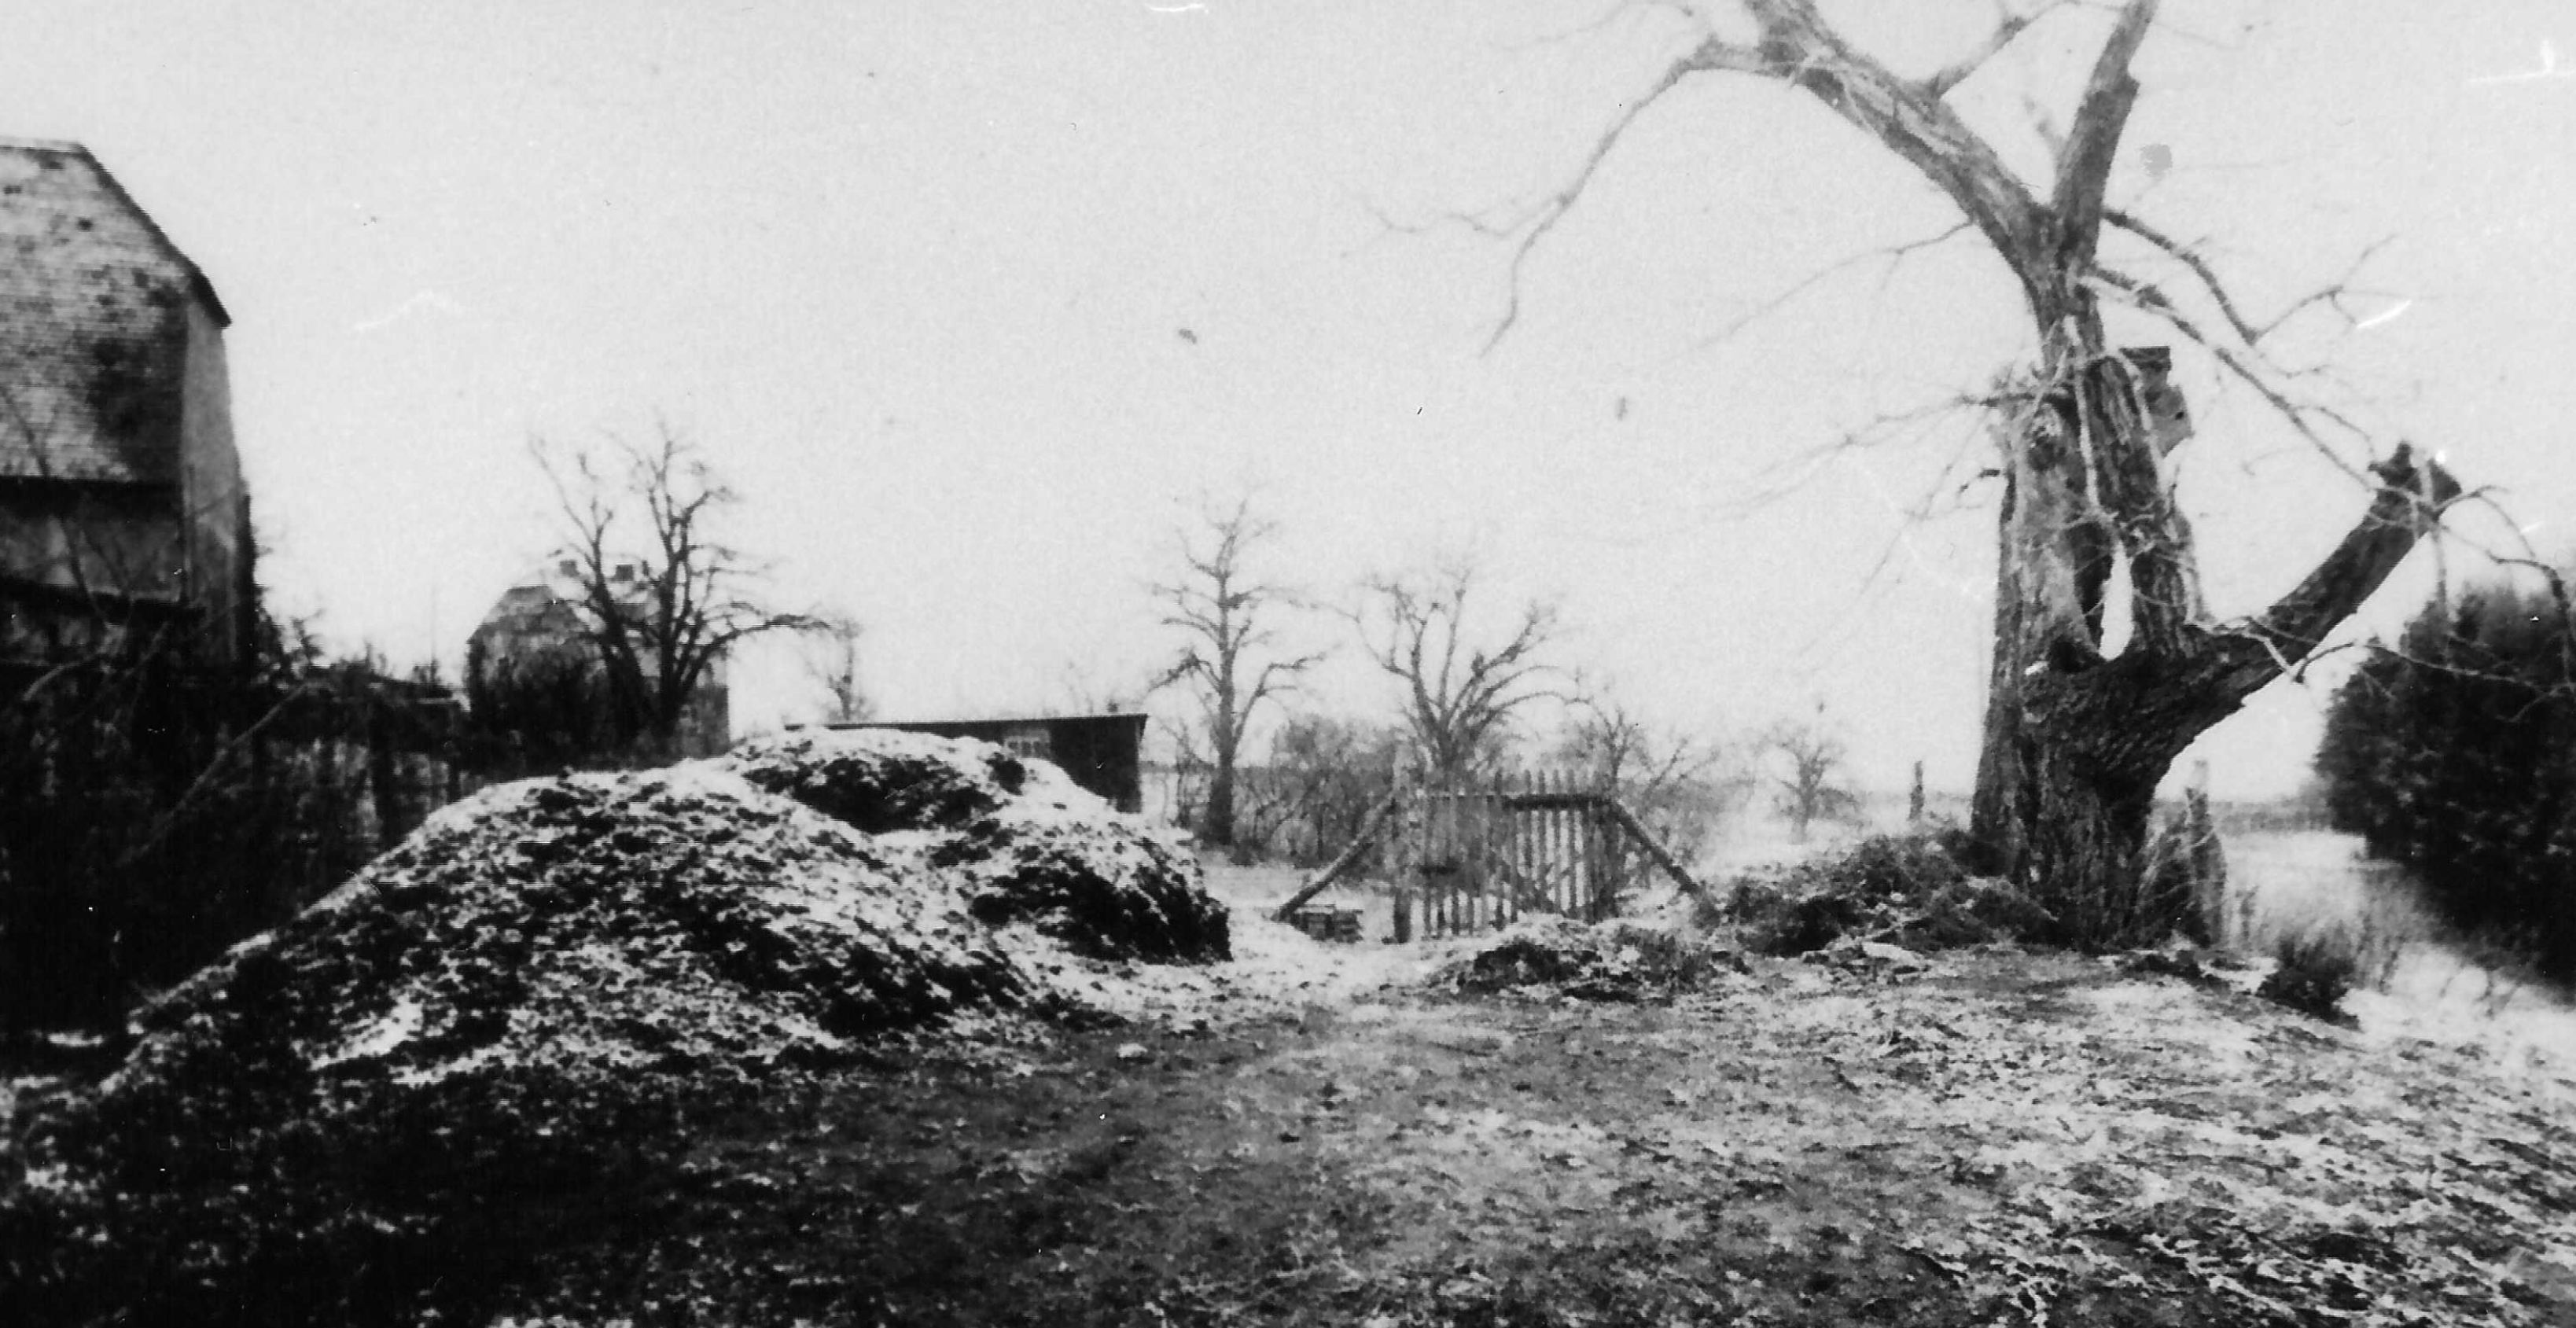
\includegraphics[width=.9\linewidth]{images/tm02}}}\\[-5pt] 

\myfigure{tm03}{BStU MFs Ast StKs 13/48 Bd.2.}{}{}{0.479}\hspace{0pt} 	&

\myfigure{tm04}{BStU MFs Ast StKs 13/48 Bd.2.}{}{}{0.043}		\\[-20pt]
 
\myfigure{tm05}{BStU MFs Ast StKs 13/48 Bd.2.}{}{}{0.479}\hspace{0pt} &

\myfigure{tm06}{BStU MFs Ast StKs 13/48 Bd.2.}{}{}{0.043} \\



\multicolumn{2}{l}{\setlength{\fboxsep}{0pt}\setlength{\fboxrule}{0pt}
\fbox{\mypics[BStU MFs Ast StKs 13/48 Bd.2.]{\noindent Leichenfunde unter dem Komposthaufen des Stadtguts}{Leichenfunde im Stadtgut Kunnerwitz (Komposthaufen)}}}
\end{tabular}
\setlength{\fboxrule}{1pt}
\newpage

\begin{tabular}{p{.45\linewidth}p{.45\linewidth}}
\myfigure{tm07}{BStU}{}{}{0}		& 
\myfigure{tm08}{BStU}{}{}{0}		\\[-35pt]
\myfigure{tm09}{BStU}{}{}{0}\hspace{-35pt}		&
\myfigure{tm10}{BStU}{}{}{0}		\\[-35pt]
\myfigure{tm11}{BStU}{}{}{0}\hspace{-35pt}		& 
\myfigure{tm12}{BStU}{}{}{0}\\[-20pt]
\multicolumn{2}{l}{\setlength{\fboxsep}{0pt}\setlength{\fboxrule}{0pt}
\fbox{\mypics[BStU MFs Ast StKs 13/48 Bd.2.]{Leichenfunde an der Mauer des Stadtguts}{Leichenfunde im Stadtgut Kunnerwitz (Mauer)}}}
\end{tabular}



\paragraph{Deutsch-Paulsdorf\index{o}{Deutsch-Paulsdorf}}
In Deutsch-Paulsdorf\index{o}{Deutsch-Paulsdorf} wurden laut Hinweisen der Bevölkerung insgesamt vier getötete Häftlinge gefunden, deren Verbleib ungewiss ist. Nach Recherchen des damals in der Sache ermittelnden Kriminalkommissars Kurt Wolf\index{p}{Wolf, Kurt} lag ein Toter an der \glqq Waage\grqq~(Waage für landwirtschaftliche Güter), zwei weitere in der Nähe des Hofes von Familie Schmidt\index{p}{Schmidt} und ein Leichnam in der Sandgrube, nahe dem ehemaligen Abzweig nach Altbernsdorf\index{o}{Altbernsdorf}\footnote{Interview mit Kurt Wolf, Löbau 2005-10}.


\paragraph{Obersohland am Rotstein\index{o}{Obersohland}\label{sohland}}
Während des Aufenthalts der Gefangenen im Göbelschen\index{p}{Göbel} Gut in Obersohland\index{o}{Obersohland} starben des nachts fünf Menschen; angeblich weil sie versuchten, auf den Dachbalken der Scheune zu schlafen und herunter fielen. Jene fünf Leichen wurden an einem unbekannten Ort hinter dem Obersohländer\index{o}{Obersohland} Friedhof beigesetzt und mit keinem Wort in den Kirchenbüchern vermerkt.
\newline
In einem nahe gelegenen Waldstück kam es angeblich zu einer Erschießung von sieben Menschen. Der genaue Ort ist bis heute unbekannt\footnote{Vgl. Schlomo Graber: Schlajme. Vgl. auch Jakob Rosenbaum: Von Görlitz nach Tirol.}.


\paragraph{Lehdehäuser\index{o}{Lehdehäuser}}
Wie bereits erwähnt, waren einige Bewohner der Lehdehäuser\index{o}{Lehdehäuser} Zeuge, wie vor ihren Augen ein entkräfteter Häftling niedergeschlagen und erschossen wurde. Wahrscheinlich sammelte das \glqq Leichenkommando\grqq~den Toten später ein, denn laut Aussage eines Anwohners hinterließ die Gefangenenkolonne keine Spuren. 

\paragraph{Buschschenke\label{buschschenke}}
Gerda Bötig bezeugt einen Toten, den sie unweit vom elterlichen Haus auf der Straße liegend fand.
~\newline
Am 03. November 1947 heißt es in einem Polizeibericht, dass man auf der Verbindungsstraße Kemmnitz--Strahwalde sieben Leichen im Wald gefunden hatte (Bild ~\mypicsref{leichenwald}), \glqq welche am 26.02.1945 durch den Totenbettmeister von Kemnitz\index{o}{Kemnitz}, August Hänsch\index{p}{Hänsch, August}, auf Anordnung des damaligen Bürgermeisters von Kemnitz\index{o}{Kemnitz}, Richard Milsch\index{p}{Milsch, Richard}, an der Fundstelle beerdigt wurden.\grqq\footnote{BStU MfS ASt 13/48 Bd. 2 / 479.}. Die Exhumierung im Jahre 1947 geschah im Beisein der Großschweidnitzer Ärzte Dr. Ehrlich\index{p}{Ehrlich, Dr.} und Fräulein Dr. Elfriede Ochsenfahrt\index{p}{Ochsenfahrt, Elfriede Dr.}\footnote{xxx Zusammenhang mit Euthanansieverbechen in Großschweidnitz klären.}. Von den gefundenen sieben stark verwesten Leichen waren drei Schädel total zertrümmert, ein weiterer wies an beiden Schläfen handtellergroße Sprünge auf\footnote{BStU MfS ASt 13/48 Bd. 2 / 481.}. Bei den drei anderen Skeletten konnten die Ärzte keine sichtbaren Spuren von Gewalteinwirkung feststellen. Die Umbettung geschah am 4. November 1947; wohin, wurde nicht erwähnt.
\newline
Ferner gibt der Polizeibericht Aufschluss über die persönlichen Dinge, welche die Opfer während des Marsches mit sich führten. Neben sieben paar Holzschuhen fanden die Ermittler: \glqq 1 Tabakdose mit Inhalt eine Zigarettenspitze, 1 Ausschnitt einer Zeitung in slawischer Sprache, 5 blecherne Essschüsseln, 3 Löffel, 1 Taschenmesser und 2 feststehende Messer\grqq.

\myfigure[leichenwald]{tm13}{BStU MFs Ast StKs 13/48 Bd.2.}{Leichenfunden im Wald zwischen der Buschschenke\index{o}{Buschschenke} und Berthelsdorf\index{o}{Berthelsdorf}}{Leichenfunde im Wald}{0}

Zu den Fundstücken zählte die Polizei noch etwas wesentlich Wertvolleres, dessen sich die damaligen Machthaber in gleicher Weise bedienten, wie zuvor die SS in den Konzentrationslagern:

\begin{leftbar} 
Ferner wurden auf Anordnung der SMA [Sowjetische Militäradministration] die Gold- und Silberzähne aus den Gebissen der Toten entfernt und werden sofort nach Eintreffen in der hiesigen Dienststelle der SMA-Dienststelle Löbau/Sa. zugestellt.\footnote{BStU MfS ASt 13/48 Bd. 2 / 481.}
\end{leftbar} 
Der materielle Wert des Edelmetalls wiegt bei diesem Befehl offensichtlich schwerer als die Pietät.

\paragraph{Berthelsdorf\index{o}{Berthelsdorf}}
Es gibt Gerüchte über Leichenfunde zwischen der Neuberthelsdorfer Sandgrube und dem Oberhof (Berthelsdorf\index{o}{Berthelsdorf}), jedoch keine bestätigten Funde\footnote{Laut Hinweisen von Ilse Gießler und Wolfgang Bittrich\index{p}{Bittrich, Wolfgang} sowie einiger anderer Berthelsdorfer\index{o}{Berthelsdorf} Bürger.}. Alle innerhalb der Ortschaft verstorbenen Menschen schaffte man wahrscheinlich mittels Wagen nach Rennersdorf\footnote{Hildegard Fleischmann. BStU MfS ASt 13/48 Bd. 2 / 460.}.


\subsubsection{Opfer in Rennersdorf}
Die Zahl der in Rennersdorf zu Tode gekommenen KZ-Gefangenen ist ebenso unbestimmt wie die Opferzahl während des Todesmarsches. 

Laut dem damaligen Ortschronisten Robert Heinze\index{p}{Heinze, Robert} wurden bereits im Oktober 1945 insgesamt acht Leichen durch ehemalige Rennersdorfer NSDAP-Mitglieder freigelegt und auf den örtlichen Friedhof umgebettet\footnote{Robert Heinze: Ortschronik Rennersdorf. Dies stimmt mit der Aussage von Christa Schubert überein, deren Vater der Ausgrabungsaktion beiwohnen musste.}. Bei der Exhumierung verpflichtete die SMA eine Schulklasse aus Rennersdorf zur Anwesenheit\footnote{Aussage von Christa Schubert, deren Bruder im Kindesalter bei den Ausgrabungen anwesend war.}.

Eine andere Rennersdorfer Schulklasse machte bei einem Ausflug eine grausige Entdeckung, als beim Laufen abseits des Weges mehrere Knochen hervortraten\footnote{Edeltraud Bittrich. Interview vom 29.03.2004.}. Die daraufhin verständigte Polizei leitete weitere Ermittlungen ein.
Am Donnerstag dem 29.01.1948 kam es dann in Rennersdorf zur Ausgrabung von vier Leichen. Anwesend waren der Polizeiarzt Dr. Gottschalk\index{p}{Gottschalk, Dr.} aus Görlitz und die Kriminalkommissare Reimann\index{p}{Reimann (Kommisar)}, Wolf\index{p}{Wolf, Kurt}, Hulek\index{p}{Hulek (Kriminaltechniker)}, der stellvertretende Bürgermeister Richter\index{p}{Richter}\footnote{BStU MfS ASt 13/48 Bd. 2 / 465.}, ferner einige Arbeiter, zumeist ehemalige Mitglieder der Hitlerjugend\footnote{Laut Günter Scholze, der damals selbst mit Hand anlegen musste. Telefonisches Interview vom 29.03.2004.}.
\begin{leftbar} 
An einem etwa 2 Meter hohen Abhang befand sich die Fundstelle. Der Abhang war mit Grasbüschen bewachsen. Die Fundstelle war bei unserem Eintreffen leicht mit Erde und Stroh zugedeckt. Die Kriminalpolizei hatte bereits einige Tage zuvor mit dem Suchen begonnen. Als sie dabei auf die Knochenreste stießen, wurde die Arbeit nicht fortgesetzt, da die Kriminaldienststelle Görlitz K5 verständigt werden musste\footnote{Das erklärt, warum die Fundstelle mit Stroh und Erde abgedeckt war.}.
\newline
Nachdem von uns die Erde entfernt wurde, waren 4 Skelette von Leichen zu sehen, die in schwarze Lumpen gehüllt waren. Die Skelette lagen geschichtet nebeneinander, zwei Kopfschädel neben den Beinen und Fußknochen der beiden anderen Skelette, die in umgekehrter Richtung lagen. Beim Herausnehmen der Knochenstücke zerfielen diese sofort in einzelne Stücke, so dass der Zusammenhang verloren ging. Bei der oberflächlichen Untersuchung durch Dr. Gott-schalk\index{p}{Gottschalk, Dr.} konnten keine Schuss- oder Schlagverletzungen festgestellt werden. Die Knochenstücke wurden in Papiersäcke geborgen und im Kraftwagen nach Görlitz gebracht.\footnote{BStU MfS ASt 13/48 Bd. 2 / 465.}
\end{leftbar}
Merkwürdig erschien den Ärzten, dass sämtliche Schädel Frakturen mit glatten geradlinigen Bruchlinien aufwiesen, die eine Einwirkung eines stumpfen Gegenstandes ausschließen\footnote{BStU MfS ASt 13/48 Bd. 2 / 467.}.
Bei zwei der Leichen fehlten die Halswirbel (Atlas), was auf einen Einschuss im Genick als Todesursache schließen läßt. 
\newline
Der Verbleib dieser insgesamt zwölf Leichname in Rennersdorf ist indes nur teilweise geklärt. Laut der Grabsteininschrift sind auf dem Rennersdorfer Friedhof 10 jüdische Menschen begraben. Demnach bestattete man neben den acht, im Jahre 1945 gefundenen, Leichen, noch zwei weitere, deren Fundstelle unbekannt ist oder mit der im Februar 1948 aufgedeckten Grabstätte übereinstimmt (siehe auch S.~\pageref{leichen}).

Die Differenz zwischen den von Emmrich Schiffer dokumentierten 75 in Rennersdorf angekommenen Toten und den tatsächlich gefundenen 12 Leichnamen, konnte nicht aufgeklärt werden. Auch die im Jahre 2010 im Auftrag des Sächsischen Landesamtes für Archäologie durchgeführten archäologischen Untersuchungen des Waldstücks neben dem Pferdestall blieben ergebnislos.

\subsubsection{Todesopfer zwischen März und Mai 1945}

Bei Rückkehr der Gefangenen nach Görlitz befand sich die Stadt immer noch im Ausnahmezustand. Die Flüchtlingsströme aus Osten und die nahe liegende Front bedingten während dieser Zeit viele Todesfälle, welche die örtlichen Bestatter kaum noch bewältigen konnten. 
Im Tagebucheintrag des Görlitzer Predigers Franz Scholz\index{p}{Scholz, Franz}\footnote{Franz Scholz wurde später wegen seines couragierten Eintretens für Kriegsgefangene zum Ehrenbürger der Stadt Görlitz ernannt.} heißt es bereits am 12. Februar:
\begin{leftbar}
Die Leichenhalle auf dem städtischen Zentralfriedhof platzt aus allen Nähten. Die Toten sind dort längst nicht mehr alle unterzubringen. [...] Für die Leichen der Erwachsenen wird die riesige Halle der Nikolaikirche bestimmt.
\end{leftbar}
\newpage
Es scheint klar, dass die Einäscherung weiterer KZ-Häftlinge unter diesen Umständen unmöglich erschien\footnote{Einige Quellen berichten zudem vom Ausfall der Gasversorgung im Krematorium, dies konnte jedoch nicht weiter bestätigt werden.} und die Lagerleitung eine andere Möglichkeit finden musste, sich der fortlaufenden Todesopfer im Lager zu entledigen.
\newline
Berichte, wonach es auch im Krematorium Zittau zur Einäscherung Görlitzer Häftlinge kam, ließen sich weder widerlegen noch eindeutig bestätigen. Im Krematorium Zittau\index{o}{Zittau} sind zwischen dem 19. Februar und 7. Mai 1945 insgesamt 106 jüdische Häftlinge in den Einäscherungsbüchern verzeichnet. Mindestens 29 der dort aufgeführten Häftlingsnummern weichen nur geringfügig von den Nummern Görlitzer Häftlinge ab. Die Angaben sind aber jeweils nicht eindeutig einer Person zuzuordnen, da entweder die Häftlingsnummer oder der Name gelistet ist.
\newline
Der nur wenige hundert Meter vom Lager entfernte Jüdischen Friedhof wurde in der folgenden Zeit als notdürftiger Bestattungsort der toten Häftlinge sowie der im Lager hingerichteten Personen genutzt. Die Gefangenen mussten dafür mehrere Massengräber errichten. 
\newline
Zur Öffnung zweier Massengräber auf dem jüdischen Friedhof kam es zwischen dem 19. und 22. Februar 1948 im Zuge der Ermittlungen gegen den Görlitzer Kreisleiter Malitz\index{p}{Malitz, Dr. Bruno} und Oberbürgermeisters Meinshausen\index{p}{Meinshausen, Dr. Hans}\footnote{Laut Aussage von Kurt Wolf, welcher damals zusammen mit Kommissar Mellmann die Ausgrabungen auf dem Jüdischen Friedhof leitete. Interviews mit Kurt Wolf, Löbau 2005-10.}. 
Bei der gleichzeitigen Exhumierung der sterblichen Überreste fanden die Ermittler insgesamt 173 Leichen (Bild.~\ref{leichenzeitung}), darunter sechs Särge mit jeweils 1--3 Leichen darin. Alle übrigen Leichen fanden die Ermittler in bis zu vier Schichten übereinander gestapelt und unbekleidet in den Gräbern. Mindestens\label{weiss} drei von ihnen hatten längere Haare, was zunächst die Vermutung nahe legt, dass es sich bei ihnen nicht um Lagerinsassen handelt, sondern vielmehr um die Kriegsgefangenen, die während der letzten beiden Kriegsmonate im Lager umgebracht wurden. Dieser Schluss gilt nicht unbedingt, da insbesondere jene Frauen im Lager lange Haar trugen, die ab Januar 1945 in Görlitz eintrafen\footnote{Interview mit Anna Hyndr\'akov\'a, Prag 2005.}. 

Als bemerkenswert gilt der Fund von einer in weißes Tuch gehüllten Frau. Der Überlebende Janek Oborowicz\index{p}{Oborowicz, Janusch} bekundet, dass es sich dabei um eine Ungarin handelt, deren Leichnam er selbst gesehen hat\footnote{\glqq Der Rapportführer sagte, dass vor einigen Tagen eine Ungarin beigesetzt wurde.\grqq~Janek Oborowicz. BStU MfS ASt 13/48 Bd. 2 / 472.}. Darüber hinaus konnten die Ermittler unter den Opfern noch zwei weitere Frauen ausmachen. Einige Leichen trugen Zivilkleidung und bei zwei weiteren konnte eindeutig festgestellt werden, dass sie zum Zeitpunkt des Todes nicht älter als 19 bzw. 20 Jahre waren.
Die Polizei\linebreak\newpage stellte schließlich fest, dass einige (nicht unbedingt alle) der im Lager von der SS und Gestapo hingerichteten Kriegsgefangenen und Fremdarbeiter an keinem anderen Ort als dem Jüdischen Friedhof beigesetzt wurden\footnote{Juda Widawski. LArchB B Rep 058 Bd. 2. Siehe auch BStU MfS ASt 13/48 Bd. 2 / 549.}.
~\newline
Der damals in die Ermittlungen involvierte Polizeikommissar Kurt Wolf\index{p}{Wolf, Kurt} schreibt dazu:
\begin{leftbar}
Oberarzt Dr. Scheit\index{p}{Scheit, Dr.} vom Friedrichstädter Krankenhaus in Dresden\index{o}{Dresden} konnte anhand von Ein- und Ausschusslöchern oder Schlagverletzungen am Kopf nachweisen, dass ein großer Teil der Häftlinge nicht nur eines Hungertodes starb, sondern durch äußere und brutale Gewalteinwirkung.\footnote{Kurt Wolf: Das KZ-Außenlager Görlitz Biesnitzer Grund, S. 23.}
\end{leftbar}

\myfigure[leichenzeitung]{YV-1948-ExhumierungJuedischerFriedhof.png}{YV 951, Id: 52982.}{Presseecho zu den Leichenfunden auf dem Jüdischen Friedhof.}{Presseecho zu den Leichenfunden auf dem Jüdischen Friedhof.}{0}

\hspace{-8pt}
\begin{tabular}{p{.305\linewidth}p{.305\linewidth}p{.305\linewidth}}
\myfigure{jf_schaedel_3}{}{}{Jüdischer Friedhof: Schädel}{0}&
\myfigure{jf_schaedel_1}{}{}{Jüdischer Friedhof: Schädel}{0}&
\myfigure{jf_schaedel_2}{}{}{Jüdischer Friedhof: Schädel}{0}
\\[-14pt]
\multicolumn{3}{l}{\setlength{\fboxsep}{0pt}\setlength{\fboxrule}{0pt}
\mypics[BStU MFs Ast StKs 13/48 Bd.2.]{Ein zertrümmerter und zwei Schädel mit Einschussloch}{Schädelfunde auf dem Jüdischen Friedhof}}
\end{tabular}

\myfigure{jf02}{BStU MFs Ast StKs 13/48 Bd.2.}{Dr. Scheit\index{p}{Scheit, Dr.} bei der Untersuchung eines Schädels}{Jüdischer Friedhof: Dr. Scheit}{0}

\newpage
\myfigure{jf03}{BStU MFs Ast StKs 13/48 Bd.2.}{Durch Bretter abgetrenntes Massengrab}{}{0}

\myfigure{jf01}{}{Kurt Wolf (zweite v. links) mit Meinshausen\index{p}{Meinshausen, Dr. Hans} (links) und Malitz\index{p}{Malitz, Dr. Bruno} (dritte v. rechts) vor Ort.}{Jüdischer Friedhof: Angeklagte vor Ort}{0}

\myfigure{jf04}{BStU MFs Ast StKs 13/48 Bd.2.}{}{Jüdischer Friedhof: Ausgrabungen}{0}


\myfigure{jf05}{BStU MFs Ast StKs 13/48 Bd.2.}{}{Jüdischer Friedhof: Ausgrabungen}{0}

\myfigure{jf06}{BStU MFs Ast StKs 13/48 Bd.2.}{}{Jüdischer Friedhof: Ausgrabungen}{0}


\myfigure{jf07}{BStU MFs Ast StKs 13/48 Bd.2.}{}{Jüdischer Friedhof: Ausgrabungen}{0}

\myfigure{jf08}{BStU MFs Ast StKs 13/48 Bd.2.}{}{Jüdischer Friedhof: Ausgrabungen}{0}

\myfigure[BStU MFs Ast StKs 13/48 Bd.2.]{jf09}{BStU}{Umbettung der Toten in den hinteren Teil des Friedhofs}{Jüdischer Friedhof: Umbettung}{0}



\newpage
\section{Ermittlungen gegen NS-Verbrecher\label{ns-verbrechen}}
Bereits im Februar 1942 beschlossen die Alliierten auf der Konferenz von Jalta\index{o}{Jalta}, alles Mögliche zu tun, um \glqq den deutschen Militarismus und Nazismus zu vernichten und endgültig die Garantie dafür zu schaffen, dass Deutschland nie wieder dazu in der Lage sein wird, den Weltfrieden zu brechen\grqq\footnote{Vgl. Peter Reichel: Vergangenheitsbewältigung in Deutschland, S. 30. Siehe auch: Alexander Fischer (Hg.): Teheran -- Jalta -- Potsdam. Die sowjetischen Protokolle von den Kriegskonferenzen der Großen Drei, S. 184f.}. Konkretisiert wurde dieses Vorhaben durch die Direktive Nr. 24 des Alliierten Kontrollrates im Januar 1946.
Um dieses Ziel zu erreichen, sollten alle nazistischen und militärischen Einflüsse aus öffentlichen Einrichtungen, dem Kultur- und Wirtschaftsleben entfernt, und sämtliche Kriegsverbrecher angeklagt und verurteilt werden.
Die Notwendigkeit, die Straftäter des KZ-Außenlagers Görlitz vor Gericht zu stellen, wurde aber auch maßgeblich durch die ehemaligen Gefangenen forciert. Des Weiteren bestand ein erhebliches öffentliches Interesse, die zahlreichen Leichenfunde aufzuklären und die dafür verantwortlichen Personen zur Rechenschaft zu ziehen. 
In der sowjetischen Besatzungszone begannen die Ermittlungen im Zusammenhang mit dem Görlitzer KZ-Lager zwar relativ zeitig, doch ermittelte man erst im Jahre 1948 intensiver, als es darum ging, die Görlitzer \glqq Hauptkriegsverbrecher\grqq~dingfest zu machen. 
Sämtliche Ermittlungsverfahren, die in den westlichen Besatzungszonen bzw. der BRD eingeleitet wurden, basierten entweder auf Strafanzeigen ehemaliger Gefangener oder auf Hinweise polnischer Behörden, welche ihrerseits sehr konsequent gegen NS-Verbrecher vorgingen.
~\newline
Eine vergleichende Bewertung des Umgangs mit NS-Verbrechern in der DDR und der BRD lässt sich anhand der wenigen hier betrachteten Fälle jedoch nicht vornehmen und ist auch nicht das Anliegen dieses Buches. Die hier betrachteten Fälle machen dennoch deutlich, dass die Verantwortung für die Geschehnisse im KZ-Außenlager Görlitz nicht auf eine homogene Personengruppe reduziert werden kann, obwohl weder Staatsanwaltschaften noch Gerichte gewillt waren die Verstrickung zwischen Funktionshäftlingen, Lagerpersonal, Staatsorganen und Wirtschaft gebührend zu berücksichtigen. Dem entgegen steht die wahrscheinlich größere Zahl derer, die von den sowjetischen Besatzern wegen bestimmter Beziehung zum Görlitzer KZ-System ohne richterliches Urteil in sowjetischen Speziallagern wie Bautzen festgehalten wurden\footnote{Hinweis darauf geben Berichte über den Rennersdorfer Gutsverwalter Lehmann, den Fuhrparkleiter Anton Sedlak (Akten sind verschollen) sowie Männer des Wachpersonals. Vgl. BStU MfS ASt 13/48.}. 

Eine genauere Betrachtung der Ermittlungen im Zusammenhang mit dem KZ-Außenlager Görlitz erfolgt anhand der einzelnen Fälle. 

\newpage
\paragraph{Der Lagerkommandant Erich Rechenberg\index{p}{Rechenberg, Erich}\label{rechenberg_ahndung}}
Die Flucht Rechenberg\index{p}{Rechenberg, Erich}s misslang am 11. Mai 1945 in Deutsch-Gabel\index{o}{Deutsch-Gabel} (Jablonné v Podještědí, Tschechien), wo er und einige Wachleute in die Arme der Roten Armee fielen. Rechenberg\index{p}{Rechenberg, Erich}
verbrachte die folgenden achteinhalb Jahre in den sowjetischen Kriegsgefangenenlagern
Hoyerswerda\index{o}{Hoyerswerda}, Frankfurt/Oder\index{o}{Frankfurt/Oder}, Rybinsk\index{o}{Rybinsk} (ab Juli 1945), Nowo Tscherkask\index{o}{Nowo Tscherkask}, Tanganrok\index{o}{Tanganrok}, Rostow\index{o}{Rostow}, Schachty\index{o}{Schachty}, Tanganrok\index{o}{Tanganrok} und zuletzt in Krasnopolje\index{o}{Krasnopolje} (bis September 1953)\footnote{LArchB B Rep 058 Bd. 2.}. Nach
seiner Rückkehr erhielt er durch die Bundesrepublik Deutschland, offenbar ganz selbstverständlich, 4140 DM Entschädigung für die Zeit seiner Gefangenschaft\footnote{Ebenda.}.
\newline
Nachdem polnische Behörden erhebliches Beweismaterial zur Verfügung stellten, begann die Staatsanwaltschaft Berlin\index{o}{Berlin} im Jahre 1970 gegen Erich Rechenberg\index{p}{Rechenberg, Erich} zu ermitteln.
Gemäß \S\,170 Abs.~2 wurde das Verfahren gegen ihn am 6. Dezember 1971 aufgrund widersprüchlicher Zeugenaussagen und fehlender Identifizierung der Person Rechenberg\index{p}{Rechenberg, Erich} durch Zeugen eingestellt. Der Name Rechenberg\index{p}{Rechenberg, Erich} war den über 100 Befragten zumeist unbekannt, nicht jedoch sein Aussehen. Bei den Rechthilfeersuchen verzichteten die Behörden auf die Beilegung von Fotos des Beschuldigten und fragten statt dessen nur nach seinem Namen. Letztlich fand sich lediglich ein belastender Zeuge, dessen alleinige Aussage allerdings nicht als ausreichend erachtet wurde und zudem teilweise im Widerspruch zu Aussagen anderer Häftlinge stand. Während des gesamten Verfahrens wurde Rechenberg\index{p}{Rechenberg, Erich} nicht ein einziges Mal zu den Vorwürfen befragt. Die Polizei tat sich sogar schwer, Herrn Rechenberg\index{p}{Rechenberg, Erich} daheim ausfindig zu machen, obwohl er seinen Wohnsitz seit den 1950er Jahren nicht änderte und zeitweilig sogar eine Anstellung im Landgericht Berlin\index{o}{Berlin} hatte. Die ermittelnde Staatsanwaltschaft versäumte es völlig, in Betracht zu ziehen, dass sich Rechenberg\index{p}{Rechenberg, Erich}s Verantwortungsbereich auf fünf weitere KZ-Außenlagern erstreckte, deren Überlebende nicht zu Aussagen herangezogen wurden.
~\newline
Aber was zählt schon ein Überlebender. Der Berliner\index{o}{Berlin} Oberstaatsanwalt Wolke\index{p}{Wolke} brachte es letztmalig am 20. August 1996 in einer Verfügung auf den Punkt:
\begin{leftbar} 
Was der Zeuge Schlomo Graber\index{p}{Graber, Schlomo} in Bezug auf den Beschuldigten sagen kann, ist nicht bekannt. Es dürfte kaum damit zu rechnen sein, dass er Umstände zu bekunden in der Lage ist, die zu einer Wiederaufnahme des Verfahrens führen. Dessen ungeachtet wird man wohl den Versuch machen müssen, ihn zu hören. Da die Anhörung nach Lage der Dinge sich aber nicht auf konkrete, in das Wissen des Zeugen gestellte Tatsachen stützt, sondern nur darauf beruht, dass er Überlebender des KL ist, dürfte eine förmliche Wiederaufnahme der Ermittlungen damit nicht verbunden sein.\footnote{LArchB B Rep 058 Bd. 11.}
\end{leftbar}
\newpage
Um bei Herrn Wolke\index{p}{Wolke} Gehör zu finden, bedarf es offenbar etwas mehr als das Bezeugen von Straftaten. Schlomo Graber\index{p}{Graber, Schlomo} wurde nie von deutschen Behörden zu den Verbrechen im KZ-Außenlager Görlitz befragt. Erich Rechenberg\index{p}{Rechenberg, Erich} erfreute sich eines hohen Alters und verstarb im Jahre 2000 in Ratzeburg bei Berlin\index{o}{Berlin}.


\paragraph{Lagerführer Zunker\label{zunker_ahndung}}
Über das Schicksal des Oberscharführers Zunker ist nur soviel sicher, dass er nach einer Kriegsgefangenschaft in Dachau 1947 an Polen ausgeliefert und am 25. Januar 1949, zusammen mit dem Lagerältesten Czech, in \L \'od\'z hingerichtet wurde\footnote{Prozess gegen Winfried Zunker, Az.: VII K 1613/48, VII 1614/48. Kriegsgericht \L \'od\'z.}.
Gerüchten nach war Zunker mit einer ungarischen Jüdin liiert und hat sich gemeinsam mit ihr auf die Flucht begeben\footnote{Laut Anna Hyndr\'akov\'a, die mit ihm flüchtete.}.




\paragraph{Der Lagerälteste Hermann Czech\index{p}{Czech, Hermann}\label{czech_ahndung}} 
Ein ehemaliger Häftling des KZ-Außenlagers Bunzlau\index{o}{Bunzlau} (heute: Boles\l awiec, Polen) namens Monik Mlynarski\index{p}{Mlynarski, Monik} verbrachte während der Evakuierung seines Lagers zwar nur wenige Tage im Görlitzer Lager, doch gelang es ihm den Görlitzer Lagerälteste ausfindig zu machen:
\begin{leftbar} 
Ich wollte ein Schloss in einem Erfurter\index{o}{Erfurt} Eisenwarengeschäft kaufen. Dies war nicht zu haben, deshalb wollte ich den Chef sprechen. Dieser war Czech\index{p}{Czech, Hermann}. Ich fragte, ob er Lagerältester in Görlitz gewesen sei. Er erwiderte: \glqq Alter Kollege\grqq~und bot mir eine Zigarette an. Im Hotel erzählte ich meinen Freunden davon. Diese wiederum klärten mich auf, dass Czech\index{p}{Czech, Hermann} der schlimmste Verbrecher sei und Frauen vergewaltigt hatte. Daraufhin habe ich Czech\index{p}{Czech, Hermann} bei der Polizei angezeigt.\footnote{Telefonisches Interview mit Monik Mlynarski vom 18.11.2004.}
\end{leftbar}

Ein von ehemaligen Häftlingen aufgesetztes Schreiben führte 1947 zur Verhaftung Hermann Czech\index{p}{Czech, Hermann}s:

\begin{leftbar}Berlin-Schlachtensee\index{o}{Berlin}, 22. Februar 1947:\\ 
Die unterzeichneten ehemaligen KZ-Häftlinge des KZ-Lagers Görlitz bitten die Behörden hiermit, die Verhaftung des\newline
Hermann C Z E C H\index{p}{Czech, Hermann}\\
geb. 27.10.1892\\ 
in Breslau\\
jetzt Wohnhaft in Erfurt\index{o}{Erfurt}, Zeitlitzerstr. 12, b/Herrn Zenser vorzunehmen.\newline
Dieser Hermann Czech\index{p}{Czech, Hermann} war im KZ-Lager Görlitz bis März 1945 als Berufsverbrecher Lagerältester. In dieser Eigenschaft hat er alles getan, um die Häftlinge für jede Kleinigkeit zu quälen und zu ermorden. Er hat beim Lagerkommandanten die Erschießung von unzähligen Häftlingen veranlasst. Er selbst hat täglich die Häftlinge für jede Kleinigkeit durchgepeitscht und gequält, hat das Essen, was für Lagerinsassen bestimmt war, für eigene Zwecke und für seine Leute genommen. Sein Vermögen hat er durch Diebstahl von Kleidern, Lebensmitteln, sowie Zigaretten, die für die Häftlinge bestimmt waren, erworben. Er war der grausamste Sadist, der seine Freude an der Quälerei und Ermordung der Häftlinge hatte. Kranke Häftlinge hat er aus dem Revier genommen und sie zur Arbeit gejagt, von der sie nicht mehr zurück kamen. Dagegen hat er seine Kapos und Mithelfer geschützt und sie damit zu weiteren Schandtaten angespornt. Die Zuteilung von Lebensmitteln und Zigaretten, welche die Häftlinge für ihre Arbeit von der Firma WUMAG bekommen sollten, hat er verschoben und die Häftlinge verhungern lassen.\footnote{PMGR 70/4593/MF.}
\end{leftbar}
Izaak Weintraub\index{p}{Weintraub, Izaak}, Bernard Rus\index{p}{Rus, Bernard} und Leon Hecht\index{p}{Hecht, Leon} veranlassten durch ihre Aussagen bei der Polish War Crimes Mission in Bad Salzuflen\index{o}{Bad Sulzuflen} einen Auslieferungsantrag nach Polen. Am 20.7.1947 wurde er schließlich dorthin ausgeliefert und 1948 zusammen mit dem ehemaligen SS-Lagerfüher Zunker vor dem Kriegsgericht in \L \'od\'z\index{o}{\L \'od\'z} zum Tode verurteilt\footnote{Prozess gegen Hermann Czech\index{p}{Czech, Hermann}, Az.: VII K 1613/48, VII 1614/48. Kriegsgericht \L \'od\'z.}.
Die Vollstreckung des Urteils erfolgte am 27. Januar 1949.

\paragraph{Die Lagerkapos\label{kapos_ahndung}}
Einen Tag vor der Befreiung des Lagers hatte sich der Lagerkapo Jacob Tannenbaum nach Italien abgesetzt, wo er mit importierten Schwarzmarktgütern Geschäfte machte. In Florenz lernte er seine zweite, 20 Jahre jüngere Frau kennen, mit der er später drei Kinder hatte. Der \emph{Displaced Persons Act} ermöglichte Tannenbaum\index{p}{Tannenbaum, Jacob} im Dezember 1949 die Einreise in die USA. Sechs Jahre später, im März 1955, erkannte man ihm die amerikanische Staatsbürgerschaft zu\footnote{Bekanntgabe des \glqq United States Department of Justice\grqq~vom 12. Mai 1987.}. 
In New York arbeitete er in der Folgezeit bei einem Lebensmittelgroßhändler. Seine aktive Mitgliedschaft in der orthodoxen Jüdischen Gemeinde \emph{Temple Beth El} in Manhattan Beach verlieh ihm Anonymität, da ihre Mitglieder von den übrigen orthodoxen Gemeinden relativ isoliert waren.\newline

Nachdem die USA über 35 Jahre lang Kriegsverbrecher in der Mitte der Gesellschaft ignoriert hat, gründete das Justizministerium 1979 das \emph{Office of Special Investigations} (OSI). Dieses befasste sich mit Tannenbaum, welcher 1978 duch einen ehemaligen Görlitzer Häftling angezeigt wurde. Der Fall verzögerten sich jedoch bis in die späten 1980er Jahre aufgrund der außergewöhnlichen ethischen Komplexität, den Schwierigkeiten an dutzende Zeugenaussagen aus aller Welt zu gelangen und den Vorgesetzten, die sich schwer damit taten, einen Juden eines Kriegsverbrechens anzuklagen. Ihm wurde vorgeworfen, als Aufseher in einem NS-Konzentrationslager an der Verfolgung und Inhaftierung von Menschen, aufgrund ihrer Rasse oder Religion, beteiligt gewesen zu sein. In der Pressemeldung des OSI werden Tannenbaum brutale körperliche Misshandlungen an Häftlingen vorgeworfen. Es handelte sich um einen Zivil-, nicht jedoch um ein Strafprozess, bei dem es darum ging, Tannenbaum auszubürgern und abzuschieben. Während der Verhöre durch die beteiligten Anwälte verlor Tannenbaum mehrmals das Bewusstsein. Ärzte attestierten ihm Herz- und Kreislaufbeschwerden. Angesichts seiner gesundheitlichen Verfassung ersuchte man, um seines Lebens Willen, keine Abschiebung. Die US-Regierung beließ es dabei, da Tannenbaum seine staatsbürgerlichen Rechte, d.h. seine US-amerikanische Staatsbürgerschaft freiwillig abgab. In ähnlichen Fällen hatten die USA bereits John Demjanjuk\index{p}{Demjanjuk, John} nach Israel und Karl Linnas\index{p}{Linnas, Karl} an die UDSSR ausgewiesen. Tannenbaum hätte ein ähnliches Schicksal ereilt, wenn man ihn unmittelbar nach der Anzeige des Falls -- als er sich noch bester Gesundheit wägte --  verurteilt hätte
Der ambivalente Fall Tannenbaum\index{p}{Tannenbaum, Jacob} erregte internationales Aufsehen in den Medien und bei jüdischen Organisationen\footnote{Ebenda. Vgl. auch: Schlomo Graber: Schlajme, S. 82. Der Konflikt wurde 2003 von Jeffrey Sweet im Theaterstück \glqq The Action Against Sol Schumann\grqq~thematisiert und am \emph{Victory Gardens Theatre} Chicago uraufgeführt.}. Tannenbaum spendete Zeit seines Lebens an das \emph{Simon Wiesenthal Center} in Los Angeles.\footnote{David van Biema: Poisoned Lives.} 
~\newline
Der zweite Lagerkapo, Schneebaum\index{p}{Schneebaum}, soll unter anderen Namen in den USA untergetaucht sein.






\paragraph{Der Blockälteste des Block 8: Adolf Eichner\index{p}{Eichner, Adolf}\label{eichner_ahndung}}
\glqq Sechs Jahre Haft wegen Körperverletzung mit Todesfolge und 6 Jahre Entzug bürgerlicher Ehrenrechte unter Anrechnung der Untersuchungshaft\grqq, lautete das Urteil eines Hamburger\index{o}{Hamburg} Gerichts gegen den Angeklagten Adolf Eichner\index{p}{Eichner, Adolf}\footnote{Landgericht oder Schwurgericht Hamburg 511106 (06.11.1951) Az.: (50) 13/51.}. Auf der Hamburger\index{o}{Hamburg} Reeperbahn erkannten ihn Zeugen, die er zunächst mit Geld bestechen wollte. Der zuvor mehrmals wegen Hehlerei straffällig gewordene Eichner\index{p}{Eichner, Adolf} war der Polizei bereits bekannt.


\paragraph{Kreisleiter und Oberbürgermeister der Stadt Görlitz}~\\
Durch den Befehl Nr. 201 der Sowjetischen Militäradministratur (SMAD) wurde im August 1947 die Umsetzung der Entnazifizierung im Sinne der Direktive Nr. 24 und Nr. 38 dem Dezernat K5 der Kriminalpolizei übertragen. Die K5-Kommissariate bildeten ab 1949 den Kern der Hauptverwaltung zum Schutz der Volkswirtschaft und legten zudem den dokumentarischen Grundstock für das NS-Sonderarchiv des Ministeriums für Staatssicherheit (MfS). Demzufolge sind die K5-Kommissariate ein Vorläufer des MfS\footnote{Vgl. Henry Leide: NS-Verbrecher und Staatssicherheit.}. Diese vermeintliche Randnotiz ist nicht unerheblich für die Betrachtung des Verfahrens gegen die zwei \glqq hauptschuldigen NS-Verbrecher\grqq~in Görlitz. Gemeint ist der im Volksmund bekannte Malitz\index{p}{Malitz, Dr. Bruno}-Meinshausen\index{p}{Meinshausen, Dr. Hans}-Prozess gegen Dr. Bruno Erwin Fritz Malitz\index{p}{Malitz, Dr. Bruno}, so der vollständige Name des ehemaligen NSDAP-Kreisleiters in Görlitz, und gegen den ehemaligen Görlitzer Oberbürgermeister Dr. Hans Friedrich August Meinshausen\index{p}{Meinshausen, Dr. Hans}. Malitz\index{p}{Malitz, Dr. Bruno} und Meinshausen waren zwei von insgesamt 2.405 so genannten hauptschuldigen NS-Verbrechern, gegen die in der Sowjetischen Besatzungszone zwischen September 1947 und Jahresende 1950 ermittelt wurde. Beide Beschuldigte waren jedoch zu Beginn der Ermittlungen noch nicht in polizeilichem Gewahrsam\footnote{Ebenda}.

\myfigure[anklage]{nk02}{BStU MFs Ast StKs 13/48 Bd.2.}{Meinshausen und Malitz\index{p}{Malitz, Dr. Bruno} auf der Anklagebank}{}{0}

Malitz\index{p}{Malitz, Dr. Bruno} hatte Görlitz am späten Abend des 7. Mai 1945 verlassen und flüchtete über Friedland\index{o}{Freidland} (heute: Frydland, Tschechien), Teplitz-Schönau\index{o}{Teplitz-Schönau} (heute: Teplice, Tschechien) und Chemnitz\index{o}{Chemnitz} nach Goslar im Harz\index{o}{Goslar / Harz}\footnote{BStU MfS ASt 13/48 Bd. 2 / 114 und 90.}. Unter Leugnung seiner Parteizugehörigkeit bekam er bereits am 26. Juli desselben Jahres eine Stelle als Abteilungsleiter im Bremer\index{o}{Bremen} Ernährungsamt, die er bis zu seiner Ergreifung am 24.02.1947 behielt\footnote{BStU MfS ASt 13/48 Bd. 2 / 114.}. Eine ehemalige Görlitzerin hatte ihn dort jedoch wiedererkannt\linebreak\newpage und bei der Polizei angezeigt, woraufhin Malitz\index{p}{Malitz, Dr. Bruno} in die Sowjetische Besatzungszone ausgeliefert wurde. 
~\newline
Meinshausen\index{p}{Meinshausen, Dr. Hans} saß indes in einem Darmstädter\index{o}{Darmstadt} Internierungslager ein und wurde auf Drängen der Stadt Görlitz ausgeliefert. Laut dem damaligen Generalstaatsanwalt Rolf Helm ist das der einzige Fall, in dem geflüchtete NS-Verbrecher aus der westlichen Besatzungszone in die sowjetische Besatzungszone zur Verurteilung überführt wurden\footnote{Vgl. Rolf Helm: Anwalt des Volkes -- Erinnerungen. S. 170f.}.
\newline
Die Hauptverhandlung der Großen Strafkammer Görlitz (Bild ~\mypicsref{gerichtssaal}) in der Sache Malitz-Meinshausen begann am 6. April 1948. Auf der Anklagebank saßen der Görlitzer Oberbürgermeister Meinshausen\index{p}{Meinshausen, Dr. Hans} und der NSDAP-Kreisleiter Malitz\index{p}{Malitz, Dr. Bruno} (Bild ~\mypicsref{anklage}).

Sie wurden beschuldigt, die Sprengung von Neißebrücken, Wasserwerken und Backöfen einen Tag vor Kriegsende veranlasst zu haben. Ferner befehligten sie die Erschießung von Deserteuren, Zwangsarbeitern und Kriegsgefangenen durch den Görlitzer Volkssturm (Werksvolkssturm WUMAG) bis in die letzten Kriegstage hinein. Hinzu kommt die Anordnung zur Erschießung des Leiters des Wirtschaftsamtes Breslau\index{o}{Breslau} auf Weisung des Gauleiters Hanke\index{p}{Hanke, Karl} und vieles andere mehr.
Maßgeblich schrieb man beiden jedoch die Schuld für die Zwangsevakuierung der Görlitzer Bevölkerung sowie des sogenannten Konzentrationslagers im Biesnitzer Grund zu. \glqq [Sie] trieben 70 000 Menschen ohne Verpflegung und Transport zwangsweise auf die Landstraße. Viele Hunderte kamen um, Kinder wurden auf der Straße geboren, Alte und Kranke wurden dem sicheren Tod übergeben\grqq\footnote{RAG, Sammlungsgut KZ Biesnitzer Grund}, heißt es da in einem Zeitungsbericht\footnote{Anklageschrift vom 29.02.1948 gegen den ehemaligen Kreisleiter der NSDAP Dr. Bruno Malitz und den ehemaligen Oberbürgermeister Dr. Hans Meinshausen. Aktenzeichen: 5-5-61/333/47/201. Privatbesitz des Autors.}. Malitz\index{p}{Malitz, Dr. Bruno} berief sich in seiner Verteidigung hierbei auf eine Anordnung des stellvertretenden Gauleiters Müller\index{p}{Müller (stellvertretender Gauleiter Niederschlesiens)}, welcher unter anderem die Evakuierung befohlen haben soll\footnote{BStU MfS ASt 13/48 Bd. 2 / 170.}. Die Räumung des KZ-Außenlagers, führte Malitz\index{p}{Malitz, Dr. Bruno} an, sei auf Veranlassung der WUMAG geschehen\footnote{BStU MfS ASt 13/48 Bd. 2 / 172.}.\newline 
Aufmerksamkeit erregte der Prozess nicht nur in Görlitz, sondern dank einer weitreichenden Medienkampagne auch in der gesamten sowjetischen Besatzungszone (Bild~\mypicsref{medien})\footnote{Das Prozessgeschehen dokumentierten unter anderem die Lausitzer Rundschau, die Märkische Union (Potsdam), Die Union (Dresden) und der Tagesspiegel (Berlin).}. Der 2.000 Menschen fassende Saal der Görlitzer Stadthalle diente als Verhandlungsort, genügte jedoch kaum dem Andrang der interessierten Bevölkerung. Mittels Lautsprecher konnte die Verhandlung auch auf Görlitzer Hauptstraßen verfolgt werden\footnote{Vgl. Rolf Helm: Anwalt des Volkes -- Erinnerungen. S. 170.}. Strittig bleibt, in wie fern es sich hierbei um ein faires Verfahren\footnote{Ein \glqq faires Verfahren\grqq~gründet auf Waffengleichheit zwischen Staatsanwaltschaft und Beschuldigten, vgl. Creifelds Rechtswörterbuch, München 2007 (19. Auflage), S. 403, zitiert in Schmeitzner: Der Fall Mutschmann, S129f. Anforderungen an einen fairen Prozess: 
a) menschenwürdige Voruntersuchung (d.h. ohne Folter), b) Zulassung von Strafverteidigern (Wahl- bzw. Pflichtverteidigern), c) Zulassung von Zeugen der Verteidigung, d) Zulassung der Öffentlichkeit, e) Anwenden von Rechtsgrundlagen, die den tatvorwürfen entsprechen, f) Unabhängigkeit der Richter (vor allem von politisch-ideologischen Vorgaben), g) Individueller Schuldnachweis, h) zeitlich angemessener Verfahrensablauf, i) Anwendung eines Strafmaßes, was der Tat angemessen erscheint, j) Berufungsungs- und Begnadigungsrecht.} oder um einen Schauprozess handelte, dessen Urteil, um einer öffentlichen und vor allem deutschlandweiten Blamage zu entgehen, schon von vorn herein feststand.\newline 



Die beiden Angeklagten wurden zum Tode verurteilt. \glqq Das Strafmaß für Meinshausen sei im Verhältnis zu Urteilen des Nürnberger Militärgerichts nicht gerechtfertigt\grqq, hieß es im Revisionsantrag der Verteidigung. Die Ankläger, unter der Leitung von Generalstaatsanwalt Dr. Rolf Helm\index{p}{Helm, Dr. Rolf}, definierten daraufhin ihre Auslegung der \glqq Verbrechen gegen die Menschlichkeit\grqq, wonach ebendiese sich nicht allein auf körperliche Mißhandlung beschränken, sondern \glqq die gesamte Tätigkeit des Nationalsozialismus auf allen Lebensgebieten\grqq~einbeziehen\footnote{Entsprechend der Bestimmungen des Kontrollratsgesetzes Nr. 10.}.
Eben diese Tätigkeit stand in Bezug auf das KZ-Außenlager jedoch in Abhängigkeit mehrerer Instanzen, welche man zur Klärung der Verantwortung für den Todesmarsch hätte heranziehen müssen. Die Staatsanwaltschaft bemühte sich nicht, eine Auslieferung des Lagerkommandanten oder des Generaldirektors\index{p}{Geerling, Conrad} der WUMAG zu erwirken. Malitz\index{p}{Malitz, Dr. Bruno} und Meinshausen\index{p}{Meinshausen, Dr. Hans} wurde die gesamte Verantwortung zugeschrieben, so dass sich weitere Ermittlungen in der hier betreffenden Sache erübrigten\footnote{Ausgenommen hiervon: Gerhardt Anton Sedlak, der Fuhrparkleiter der WUMAG, den man aufgrund der Mißhandlungen, die er an Häftlingen verübte, zu acht Jahren Gefängnis verurteilte. Sedlak schwärzte Häftlinge an, die sich Schweinefutter aus den Kübeln der WUMAG holten. LG/BG Bautzen 480626 Az.: 9a/ StKs16/48, OLG Dresden Az.: 21ERKs221/48 (Akten sind verschollen). \\ Rudolf Müller verurteilte man zu drei Jahren Haft wegen Misshandlungen von Häftlingen in seiner Funktion als Meister in der WUMAG. LG/NG Bautzen 480117 Az.: 9a/StKs6/7. \\
Diese Akten sind ebenfalls nicht mehr auffindbar.}.
~\newline
Nachdem der Antrag auf Revision abgelehnt und das Gericht am 24.04.1948 das Todesurteil fällte wurden Malitz\index{p}{Malitz, Dr. Bruno} und Meinshausen\index{p}{Meinshausen, Dr. Hans} nach Ablehnung der Gnadengesuche durch die sächsische Staatsregierung am 19. Oktober 1948 in Dresden hingerichtet. 
~\newline
Alles mit dem Prozess in Verbindung stehende Aktenmaterial\footnote{Laut Aussage von Kurt Wolf (Löbau, 06.02.2009) umfasste das Material 12 Akten mit je zwei Leitzordnern.} nahm das MfS 1955 in Beschlag und stand fortan nur bedingt für gerichtliche und historische Ermittlungen zur Verfügung.
Das MfS sicherte sich diesen Fundus zum Zwecke ihres operativen Geschäfts in der BRD und begegnete Rechtshilfeersuchen seitens der westdeutschen Staatsanwaltschaften, wie etwa in der Sache Rechenberg\index{p}{Rechenberg, Erich}, nur äußerst selektiv und ausweichend.

\begin{tabular}{p{.465\linewidth}p{.465\linewidth}}
\myfigure[gerichtssaal]{MMP_11}{}{Gerichtssaal in der Stadthalle.}{}{.83}		&
\myfigure[richter]{MMP_13}{}{Der verantwortliche Richter.}{}{.81}\\[20pt]
\end{tabular}

\begin{tabular}{p{.465\linewidth}p{.465\linewidth}}
\myfigure[zeuge]{MMP_9}{}{Der Zeuge Janusch Oborowicz.}{}{.83}		&
\myfigure[medien]{MMP_8}{}{Medienvertreter.}{}{.83}\\[20pt]
\end{tabular}



 
\chapter{Gedenken und Erinnerung der Opfer}


Gedenken heißt im Kontext dieses Buches, sich der menschlichen Opfer der KZ-Außenlager Görlitz und Rennersdorf zu erinnern und sich das ihnen zugefügte Leid zu vergegenwärtigen. 
Erinnerung setzt voraus, die Umstände und Ursachen des Geschehenen kritisch zu erfassen und im historischen Rahmen zu sehen, ohne diesen Gegenstand auf die Opfer- und Gefangenenzahl zu reduzieren. Auch dann, wenn kein Zeitzeuge mehr seine mahnende Stimme erheben kann, braucht es eine öffentliche Form der Erinnerung, um die Schuld und Schuldenlast im Gedächtnis zu bewahren und vor einer Wiederholung -- ganz gleich wo auf dieser Welt -- zu warnen. 
\\
Leider wurde die Historie der KZ-Außenlager in der Nachkriegszeit weder in Görlitz noch in Rennersdorf genügend aufgearbeitet, so dass dem Aufbau und der Pflege einer Erinnerungskultur teilweise die Grundlage fehlte. Um so wichtiger erscheint es, nach dem Fall des so genannten Eisernen Vorhangs und im Zeitalter einer zunehmend vernetzten Welt, die Erinnerungsarbeit voranzutreiben und sich dabei einer Vielzahl von Medien zu bedienen. Die bisher geleistete Arbeit wird hier, wenn auch nur ausschnitthaft, dargestellt. Die zukünftig zu entwickelnden Konzepte zur Etablierung einer angemessenen Gedenk- und Erinnerungskultur sollen in dieser Dokumentation lediglich angedeutet werden.
~\newline
Eine öffentliche Form des Gedenkens an die Opfer unter den Görlitzer KZ-Häftlingen gab es lange Zeit nur in Görlitz und Rennersdorf. 
In den Jahren 1985, 1986 und 1995 wurden auf dem Gelände der Gedenkstätte Groß-Rosen unter anderem drei Tafeln (Bild ~\mypicsref{tafelgr}) zur Erinnerung an die Nebenlager in Görlitz, Kunnerwitz\index{o}{Kunnerwitz} und Rennersdorf angebracht. Letztere Gedenktafel weihte man im Beisein jugendlicher Vertreter der Rennersdorfer Kirchgemeinde sowie des Lehrers und Zeitzeugens Joachim Löwe\index{p}{Löwe, Joachim} am 6. Mai 1995 ein.\newline

Anlässlich eines Gedenkmarsches zum 60. Jahrestag der Befreiung des KZ-Außenlagers Görlitz, gibt es nun auch in Deutsch-Paulsdorf eine Gedenktafel, die an die Opfer während des Todesmarsches erinnert.\newline

Verschiedentlich findet sich in der Literatur auch der Vermerk über eine Gedenkstätte in Friedersdorf, wo vier Görlitzer Häftlinge beerdigt worden seien. Dabei handelt es sich jedoch um eine Verwechslung mit dem gleichnamigen Ort bei Neugersdorf\index{o}{Neugersdorf}, den gleichfalls 1945 ein Todesmarsch passierte\footnote{Auf einer beiliegenden Karte ist das Friedersdorf bei Görlitz richtig eingezeichnet, doch im Text ist von einem Friedersdorf\index{o}{Friedersdorf} im Kreis Löbau-Zittau die Rede. Vgl. Bundeszentrale für Politische Bildung: Gedenkstätten für die Opfer des Nationalsozialismus II, S. 668.}.

\myfigure[tafelgr]{grossrosen}{}{Die Gedenktafeln auf dem Gelände des ehemaligen KZ Groß-Rosen}{}{0}

\paragraph{Görlitz}
In der Stadt Görlitz gibt es eine ganze Reihe von Gedenkstätten für die Opfer des Nationalsozialismus, davon zwei für das KZ-Außenlagers im Biesnitzer Grund. 
In unmittelbarer Nähe zum ehemaligen Lager, auf der Fröbelstraße (Bild ~\mypicsref{froebel}), befindet sich ein Gedenkstein, welchen Schüler der damaligen 12. Polytechnischen Oberschule (POS) unter Mithilfe von \glqq Lehrern, Mitgliedern des Elternbeirates und Werktätigen des Patentbetriebes Görlitzer Maschinenbau\grqq\footnote{R. Otto. Die Verfolgung der Juden in Görlitz unter der faschistischen Diktatur
1933-1945. Stadtverwaltung Görlitz, Görlitz, 1990.}  gemeinsam errichteten. Am 8. Mai 1959 wurde der Gedenkstein unter starker Anteilnahme der Görlitzer Bevölkerung eingeweiht. Der Stein wird von einer Opferschale abgeschlossen und steht innerhalb einer steinernen, halb runden Begrenzung. Die Inschrift auf dem Stein entspricht der damaligen politischen Intention: \glqq Pionierehrenmal Schule Nr. 12 / für die Opfer des / Faschismus des KZ / Biesnitzer Grund / Ihr seid uns Vorbild und Verpflichtung\grqq\footnote{Vgl. Bundeszentrale für Politische Bildung: Gedenkstätten für die Opfer des Nationalsozialismus II, S. 671.}. Es handelt sich nicht etwa um ein Mahnmal für die Pioniere der POS, sondern um eines von denselben. Im Jahre 2003 wurde der Gedenkstein unter Beibehaltung der Inschrift mit der irreführenden Ortsangabe \glqq KZ Biesnitzer Grund\grqq saniert und an gleicher Stelle belassen, während innerhalb der Kleingartenanlage \glqq Biesnitzer Grund\grqq~ überhauptnichts an das Lager erinnert. 

\myfigure[judfriedeinweihung]{nk01}{RAG Sammlungsgut Biesnitzer Grund.}{Einweihung des Gedenksteins auf dem Jüdischen Friedhof am 13. November 1951}{Einweihung des Gedenksteins auf dem Jüdischen Friedhof}{0}

Ein weiterer Gedenkstein (Bild~\mypicsref{judfried})\label{leichen} befindet sich nur wenige hundert Meter entfernt, auf dem Jüdischen Friedhof an der Biesnitzer Straße. Ein Davidstern (Magen David) krönt den etwa zwei Meter hohen Stein. Auf der Vorderseite findet sich unter einem abgesetzten Winkel die deutsche Inschrift: \glqq Hier ruhen 323 ermordete Kameraden / die im Konzentrationslager / Biesnitzer Grund Görlitz / in den Jahren 1943 -- 1945
der Hitler Tyrannei zum Opfer fielen / Wir werden sie nie vergessen / indem wir für den Frieden kämpfen! / Die Bürger der Stadt Görlitz\grqq.\newline
Die ehemals 148 auf dem städtischen Friedhof beigesetzten Urnen fanden 1948, nach einer Umbettung auf den Jüdischen Friedhof ihre letzte Ruhestätte.  Die Zahl der Ermordeten ergibt sich wie folgt\footnote{Einäscherungsbücher der Friedhofsverwaltung Görlitz.}:
\begin{itemize}
\item 111 Urnen von namentlich bekannten Häftlingen des KZ-Außenlager Görlitz; 
\item 19 Urnen aus dem KZ-Außenlager Hartmannsdorf\index{o}{Hartmansdorf} (heute: Miloszow, Polen)
\item 13 Urnen aus dem KZ-Außenlager Niesky\index{o}{Niesky}\footnote{Vgl. Dieter Rostowski / Marlies Röhle: Vom KZ-AL Niesky nach Brandhofen (Spohla). Warum ein Dorf bei Hoyerswerda 1945 geschichtsträchtig wurde.}
\item 4 Urnen aus dem Bautzner\index{o}{Bautzen} KZ-Außenlager\footnote{Vgl. VEB Waggonbau Bautzen (Hrsg): Wag­gon­bauer pfle­gen re­vo­lu­tio­näre Tra­di­tio­nen. Aus der Ge­schichte des KZ-Außenlagers in der Maschinen- und Wag­gon­fa­brik vorm Busch Baut­zen.}
\item 173 namenlose Tote aus den Massengräbern auf dem Jüdischen Friedhof;
\item 2 unbekannte Görlitzer Häftlinge, die (wahrscheinlich) in Rennersdorf starben;
\end{itemize}
Eine Urne eines sowjetischen Kriegsgefangenen, den man am 21. April 1945 in Görlitz exekutierte, soll ebenfalls auf dem Jüdischen Friedhof bestattet worden sein\footnote{Vgl. Kurt Wolf: KZ-Außenlager Görlitz Biesnitzer Grund, S. 23.}. 
Demnach stehen nur 284 der 323 dort beigesetzen Häftlinge in Zusammenhang mit dem KZ Außenlager Görlitz. Zusammen mit den 36 Opfern anderer Lager ergibt sich die Zahl von 320 Toten, rechnet man den einen Kriegsgefangenen mit ein, bleibt immer noch eine Differenz von zwei. Die Antwort auf diese Frage findet sich aller Wahrscheinlichkeit nach in Rennersdorf.

148 Namen von Opfern sind der Friedhofsverwaltung jedenfalls seit 1948 bekannt. Aufgrund der Tatsache, dass alle 323 Leichname bzw. Urnen 1948 erneut in ein Massengrab anstatt in Einzelgräbern gebettet wurden, wirft die Frage auf, in welcher Weise man den zumeist jüdischen Opfern gedenken kann. Ein Nachfahre eines Opfers, der selbst die Shoa überlebte, musste jüngst selbst Hand anlegen (siehe Abb. \ref{MosesIsak}), um für seinen Vater den \emph{Kaddisch}\footnote{Jüdisches Totengebet.} sprechen zu können. Leider zeigt diese Art von \emph{memorial guerilla}, wie überfällig es ist, einen angemessenen Rahmen für das Gedenken an die Opfer herzustellen. Derzeit engagieren sich einige Bürger für eine Neugestaltung der Grabzeichen.

\myfigure[MosesIsak]{nk_hornung}{}{Gedenktafel Moses Isak Hornung}{}{0}

\hspace{-9pt}
\begin{tabular}{p{.47\linewidth}p{.47\linewidth}}
\myfigure[froebel]{nk04}{}{Das 2003 restaurierte Pionierehrenmal in der Fröbelstraße}{}{0}		&
\myfigure[judfried]{nk03}{}{Der Gedenkstein auf dem Jüdischen Friedhof}{}{0}\\[20pt]
\end{tabular}




Die Jüdische Gemeinde Dresden\index{o}{Dresden} wies die Stadtverwaltung Görlitz am 14. April 1948 auf den \glqq verwahrlosten Zustand\grqq~des Friedhofs hin, worauf die Stadtverwaltung die Pflege und Betreuung der Friedhofsanlage übernahm und den erwähnten Gedenkstein errichtete.
Im Beisein von ehemaligen Gefangenen des KZ-Außenlagers, Vertretern der Jüdischen Gemeinde Dresden und vielen Görlitzer Bürgern wurde der Gedenkstein am 13. November 1951 durch Oberbürgermeister Willi Ehrlich\index{p}{Ehrlich, Willi} eingeweiht (siehe Bild~\mypicsref{judfriedeinweihung}). 



\paragraph{Rennersdorf}
Gleich neben der Kirche, auf dem Ortsfriedhof, liegt eine kleine Grabanlage (Bild ~\mypicsref{friedrenn}), welche seit langem durch das Ehepaar Riehle gepflegt wird. Sie mahnt an die Ermordung von 10 jüdischen KZ-Häftlingen im März 1945 in Rennersdorf. 
Die Toten wurden erst 1950 auf dem Friedhof beigesetzt\footnote{Vgl. Bundeszentrale für Politische Bildung: Gedenkstätten für die Opfer des Nationalsozialismus II, S. 739.}. Der Gedenkstein aus Granit enthält den Davidstern gebildet mit dem Häftlingswinkel und flankiert mit hebräischen Buchstaben. Darunter ist zu lesen: \glqq Hier ruhen / 10 jüdische Männer / die von den SS-Horden / im März 1945 / ermordet wurden\grqq. 
\newline
Der Gedenkstein für die zehn namenlosen jüdischen Opfer wurde am 25. Juni 1950 auf dem Rennersdorfer Friedhof eingeweiht. Obwohl die Polizei in Rennersdorf 12 Leichen fand, sind aus unerklärlichen Gründen die Gebeine zweier Toter in Görlitz beerdigt worden. Verwunderlich ist gleichfalls die Existenz eines vermutlich älteren Grabsteins, auf dem in russischer Inschrift neun Juden erwähnt sind. 
\newline
Einmal jährlich gedachte man während der DDR-Zeit der Opfer des Nationalsozialismus mit einer Gedenkveranstaltung auf dem Rennersdorfer Friedhof. Bedauerlicherweise fanden sich an jenen Tagen kaum Dorfbewohner, sondern vielmehr Parteifunktionäre und auch Vertreter der Dresdner jüdischen Gemeinde ein. Die Reden waren zumeist ohne direkten Bezug auf die Vorkommnisse, von höheren Parteistellen vordefiniert\footnote{Interview mit dem ehemaligen Geschichtslehrer Joachim Löwe, der sich darum bemühte, dass die Geschehnisse im Rennersdorfer Lager nicht in Vergessenheit geraten.}.\newline

Anlässlich des bereits erwähnten Gedenkmarsches zum 60. Jahrestag der Befreiung stiftete die Gemeinde Berthelsdorf, deren Ortsteil Rennersdorf nun ist, eine Gedenktafel, welche die Marschstrecke der Gefangenen darstellt und dadurch den geschichtlichen Zusammenhang zwischen dem Grabstein und dem KZ-Außenlager Görlitz verdeutlicht. Diese Gedenktafel ist im Torbogen des Friedhofes angebracht und enthält die Inschrift: \glqq Zum Gedenken / Zur Mahnung / Im Frühjahr 1945 führte der Todesmarsch / jüdischer Häftlinge vom Görlitzer Konzentrationslager Biesnitzer Grund in unser Dorf. / Auf dieser Wegstrecke und während des Aufenthaltes / in Rennersdorf verstarben durch Entkräftung und / Gewalt der Nazidiktatur mindestens 45 von ihnen.\grqq


\myfigure[friedrenn]{friedrenn1}{}{Der Gedenkstein auf dem Rennersdorfer Friedhof}{}{0}


\section{Ausblick auf eine Erinnerungskultur ohne Steine}
Die bisweilen erfolgte Aufarbeitung der Geschehnisse im KZ-Außenlager
Görlitz und Rennersdorf bildet eine Grundlage für die\emph{ }Entwicklung
einer lebendigen Erinnerungskultur im \emph{Dreiländereck Polen -
Tschechien - Deutschland}. Lebendig meint hier, das vorhandene Wissen
durch Teilung zu mehren und angemessen zu vermitteln. 

Derzeit lassen sich zwei Probleme für eine freie Geschichtsforschung
und damit für eine aktive Erinnerungsarbeit am Gegenstand der Groß-Rosener
KZ-Außenlager identifizieren: 
\begin{enumerate}
\item Wichtige Primärquellen, wie Berichte von Überlebenden, sind in Archiven
auf der ganzen Welt unter Verschluss, d.h. nur umständlich und mit
hohem finanziellen Aufwand verfügbar. Beispielsweise hält die von
Steven Spielberg ins Leben gerufene \emph{Visual Shoah History Foundation}
über 52.000 videographische Berichte von Überlebenden der Shoah -
da\-runter 143 Berichte ehemaliger Görlitzer Häftlinge - unter Verschluss.
Eine Reproduktion eines einzigen Testimonies kostet knapp 100\,\$ respektive
15.000\,\$/Jahr für den Zugriff auf die gesamte Kollektion über das
Internet \footnote{USC. Testimony Services, 2010. \url{http://college.usc.edu/vhi/testimonyservices.php}.}. Ähnlich verhält es sich etwa mit Archivalien
bei der \emph{Bundesbeauftragten für die Unterlagen der Staatssicherheit},
dem \emph{Landesarchiv Berlin}, sowie dem \emph{Sächsischen Staatsarchiv
Dresden}.
\item Die zweite Hürde für eine freie KZ-Forschung und damit für eine aktive
Erinnerungsarbeit besteht in der mangelnden Verfügbarkeit von Sekundärquellen
in Form von Publikationen, die aufgrund ihrer geringen Auflagenstärke
heute nicht einmal mehr über den antiquarischen Buchhandel zu beschaffen
sind. 
\end{enumerate}
Ein wichter Ansatz, um die Verfügbarkeit von Quellen sicherzustellen,
besteht daher in der Offenlegung und dem freien Zugang zu einschlägigen
Datenbanken, Archivalien und wissenschaftlichen Arbeiten. Der in diesem
Ansatz innewohnende \emph{Open-Source-Gedanke} soll dazu anregen,
bestehende Forschungsarbeiten zu validieren, Desiderate zu identifizieren
und in neuen Formen medial aufzubereiten. Anstatt an der protektionistischen
Quellenhandhabung festzuhalten, können wir auf lokaler Ebene das historische
Wissen als Allgemeingut begreifen und den Weg für eine kritischere
Auseinandersetzung ebnen\footnote{Als erster Schritt in diese Richtung wurde die hier vorliegende und in ihrer ersten Auflage vergriffene Dokumentation der KZ Außenlager Görlitz und Rennersdorf in überarbeiteter, digitaler Form unter \emph{Creative Comons Lizenz}: \url{http://softbook.nise81.com/} zur Verfügung gestellt.}. 

Im Zeitalter einer vernetzten Welt können wir den Zugang zum dokumentierten
Geschichts\-wissen orts- und zeitunabhängig gestalten, anstatt allein
auf die wenig aktuellen und vom Informationsgehalt begrenzten steinernen
Monumente oder metallerne Tafeln zu setzen. Ein zeitgemäßes Dokumationszentrum
bestände aus einem digitalen Archiv, mit sämtlichen bekannten Quellen
und Forschungsergebnissen und einem verteilten Museum, was den ortsunabhängigen
Abruf künstlerisch und didaktisch aufbereiteter Informationen ermöglicht.
Modelcharakter besitzt das Dresdner Projekt {}``audioscript'',
in dem die Verfolgung und Vernichtung Dresdner Juden mittels frei
verfügbarer Tondokumente bzw. Audio-Guides ein räumlich verteiltes
Museum bilden\footnote{http://www.audioscript.net/}. 




 
\chapter{Zusammenfassung}
\section{Zusammenfassung}
Die Geschichte jüdischer Zwangsarbeit während des Zweiten Weltkrieges begann in Görlitz mit der Errichtung eines Zentralen Arbeitslagers der Organisation Schmelt im Frühjahr 1943. Das ZAL war eines von mindestens 23 \glqq Menschenlagern\grqq~ der \emph{Waggon und Maschinenbau AG} (WUMAG) - Görlitz' größtem Industriebetrieb und Arbeitgeber. Das ZAL wurde ursprünglich als Kriegsgefangenenlager auf dem städtischen Grundstück, unweit von Wohnsiedlungen in Form eines Barackenlagers gebaut. Mit der Auflösung der Organisation Schmelt im Frühjahr 1944 gliederte man den Görlitzer Standort dem KZ Groß-Rosen an. Die Schmelt-Häftlinge deportierte die SS in andere Arbeitslager (KZs). Das Barackenlager in Görlitz ab dem 8. August unter Leitung der SS durch Gefangene aus Groß-Rosen an die Sicherheitsstandards von KZ-Arbeitslagern baulich angepasst wurde. Bis Herbst 1944 deportierte die SS 1.500 Menschen nach Görlitz. Es waren größtenteils Juden aus Polen und Ungarn. Darunter befanden sich auch 300 Frauen, die man in einem abgetrennten Bereich des Lagers unterbrachte. 

Die Gefangenen bildeten eine heterogene Gruppe, die sich hinsichtlich ihres Alters, ihrer Nationalität und ihrer einstigen gesellschaftlichen Stellung wesentlich voneinander unterschieden, jedoch dem System und dem Terror des Konzentrationslagers, wenn überhaupt, nur schwerlich Stand halten konnten. Eine Sonderstellung galt den Funktionshäftlingen, welche die Organisation des Lagers relative autonom bestimmten und sich insbesondere durch weitgehende Privilegien von den übrigen Gefangenen unterschieden. Die Lagerleitung besetzte die Stellen der Häftlingsselbstverwaltung und duldete deren Übergriffe auf andere Gefangene sowie deren Korruptionssystem. Die meisten dokumentierten Folterungen, Misshandlungen und Vergewaltigungen werden Funktionshäftlingen zugeschrieben. Die Bewegungsfreiheit des Lagerältesten\linebreak\newpage sowie bestimmter anderer Funktionshäftlinge sorgte für einen Tauschhandel über die Grenzen des Lagers und der WUMAG hinaus. Ein Teil der unterschlagenen Lebensmittel gelangte zu den Frauen im Lager, sofern sie sich zu Gegenleistungen bereit erklärten. 

Neben der chaotischen Lagerorganisation bedingte die mangelnde medizinische Versorgung, widrige hygienische Bedingungen, schlechte Kleidung und unzureichende Ernährung eine stete Zunahme an Krankheiten und Todesfällen - vor allem unter den Männern. Auch die harte und unmenschliche Arbeit in den Werken der WUMAG trug wesentlich zur Sterblichkeit der Häftlinge bei. Abgesehen von Bonus-Rationen für überplanmäßige Arbeit sind seitens der WUMAG keinerlei Versuche bekannt, die Lebensbedingungen der Häftlinge zu verbessern. Gleiches gilt für die Lagerleitung - namentlich für den Lagerkommandanten Erich Rechenberg, dem der Kommandant des Bunzlauer Außenlagers (Hauptsturmführer Michael) im Februar 1945 den katastrophalen Umgang mit kriegswichtigen Arbeitskräften im Lager Görlitz vorwarf. Angesichts der kriegswichtigen Produktionsaufträge, welche die WUMAG zu erfüllen hatte, erscheint die zügellose Führungsrolle der SS geradezu als paradoxe Sabotage an der deutschen Rüstung. 

Eine weitere Sonderheit des KZ-Außenlagers Görlitz betrifft seine räumliche und gesellschaftliche Integration im Vergleich zu anderen Groß-Rosener Arbeitslagern. Zum einen befanden sich die Produktionsstandorte der WUMAG relativ zentral im Stadtgebiet, zum anderen grenzte das Lager unmittelbar an dicht besiedelte Wohngebiete, von denen aus die Anwohner praktisch alle Vorgänge im Lager beobachten konnten. Damit einher gingen persönliche Kontakte zwischen Einheimischen und Lagerinsassen innerhalb der WUMAG, aber auch in örtlichen Handwerksbetrieben, in den umliegenden Kleingärten und bei Besorgungen in der Stadt.     

Jeweils verheerend auf die Situation der Häftlinge im KZ-Außenlager Görlitz wirkten sich die von Alfred Konieczny beschriebenen drei Etappen der Evakuierung schlesischer KZ-Außenlager aus. In der ersten Etappe funktionierte das KZ-Außenlager als Durchgangs- und Auffanglager anderer evakuierter Lager. Während der zweiten Etappe wurde das Lager selbst über Kunnerwitz in ein provisorisches Ausweichlager nach Rennersdorf verlegt.
In der dritten Etappe kommt es zu der einmaligen Begebenheit, dass die Gefangenen im Zuge der letzten Fronterfolge der Deutschen zur Rückkehr nach Görlitz gezwungen werden, um beim Festungsausbau der Stadt eingesetzt zu werden. Die Folgen dieser letzten Verblendung der Görlitzer Kreisleitung mündeten in eine humanitäre Katastrophe, die 173 Gefangene mit ihrem Leben bezahlten. Mindestens jeder fünfte Lagerinsasse erlebte den Tag der Befreiung am 8. Mai 1945 nicht mehr.

Sowohl in der sowjetischen, als auch in den westlichen Besatzungszonen bzw. den daraus hervorgegangenen Staaten wurden Anstrengungen unternommen, die im Görlitzer KZ-Außenlager begangenen Verbrechen gegen die Menschlichkeit zu ahnden. Eine umfassende juristische Einschätzung des komplexen Verantwortungsgeflechts von SS, Funktionshäftlingen, WUMAG und \mbox{NSDAP} Kreisleitung sowie den nachgeordneten Ämtern und Institutionen kam jedoch nicht zustande. Dies lag zum einen an der Zurückhaltung relevanter Informationen durch das Ministerium für Staatssicherheit und zum anderen am Unwillen den Gesamtkomplex überhaupt betrachten zu wollen (Staatsanwaltschaft Berlin im Fall Erich Rechenberg). Insbesondere der Prozess gegen den Görlitzer Kreisleiter Malitz und Oberbürgermeister Meinshausen ist ein Beispiel für die Entlastung vieler Täter, Mittäter und Mitwisser zulasten einzelner Personen, derentwegen die öffentlichen Debatte um die Schuldfrage beendet werden konnte. Erst nach dem Fall des \glqq Eisernen Vorhangs\grqq~ und der Öffnung der Archive war es möglich, die Geschehnisse der KZ-Außenlager Görlitz und Rennersdorf aus verschiedenen Blickwinkeln kritisch zu betrachten, zu dokumentieren und insbesondere die beschriebenen Erinnerungsorte ins Bewusstsein zu rufen. 





\begin{comment}
\section{Summary} gnaz schlecht:
In Görlitz the history of jewish forced labor during World War II began with the erection of the \emph{Zentralen Arbeitslager} (ZAL) of the Organsation Schmelt in spring 1943. The ZAL was only one of XXX so called /human ware houses/ of Görlitz' biggest industrial manufacturer, the Waggon und Maschninenbau AG (WUMAG). Initially the ZAL has been a barack camp /war prisoners/ on the property of the city of Görlitz, closely to housing settlements. In Spring 1944 when the organisation Schmelt has been liquidated, the branch in Görlitz became a part of concentration camp Groß Rosen. Inmates of the former Schmelt camp were dortorted to other forced labor camps respectivly concentration camps. In the same time the Görlitz camp got under control of the SS. On 8th of August 1944 the first prisoners from KZ Groß Rosen were oblidged to enhance the security standards to the level of concentartions camps. Until autum 1944 the SS deported 1500 people to Görlitz. Most of them were jews from Poland and Hungaria. 300 of them were women and therefor accomodated in a separate part of the camp.

The inprisoners were a heterogenous group. Their age differed widly, same as their nationality and their former social status. All of them could hardly withstand the system of terror of the concentration camp. So called Funktionshäftlinge were prisoners oblidged with special duties in order to organize the camp almost independently. Therefor they were previliged in contrast to their fellow prisoners. The camp leadership put inmates in these positions of the self administration and suffer attacks as well as corruption around food and other coveted goods. Most of the documented tortures, ill-treatments and raptures could be attributed to prisoners in duty. The relativly freedo of action of the Lagerältesten (prisoner in chief) and other prisioners with special obligations encouraged bartering accross the camp borders as well as the WUMAG. The femal inmates benefit from that barter goods, if they had agreed to rewards. 

Beside the chaotic organisation of the camp ...

Neben der chaotischen Lagerorganisation bedingte die mangelnde medizinische Versorgung, widrige hygienische Bedingungen, schlechte Kleidung und unzureichende Ernährung eine stete Zunahme an Krankheiten und Todesfällen - vor allem unter den Männern. Auch die harte und unmenschliche Arbeit in den Werken der WUMAG trug wesentlich zur Sterblichkeit der Häftlinge bei. Abgesehen von Bonus-Rationen für überplanmäßige Arbeit sind seitens der WUMAG keinerlei Versuche bekannt, die Lebensbedingungen der Häftlinge zu verbessern. Gleiches gilt für die Lagerleitung - namentlich für den Lagerkommandanten Erich Rechenberg, dem der Kommandant des Bunzlauer Außenlagers (Hauptsturmführer Michael) im Februar 1945 den katastrophalen Umgang mit kriegswichtigen Arbeitskräften im Lager Görlitz vorwarf. Angesichts der kriegswichtigen Produktionsaufträge, welche die WUMAG zu erfüllen hatte, erscheint die zügellose Führungsrolle der SS geradezu als paradoxe Sabotage an der deutschen Rüstung. 
\end{comment}




\section{Streszczenie}
Historia pracy przymusowej w Görlitz (Zgorzelec) podczas drugiej wojny światowej ma swój początek wraz z uruchomieniem centralnego obozu pracy organizacji „Schmelt“ wiosną 1943 roku. Obóz ten był jednym z 25 „magazynów ludzi“ należących do  fabryki wagonów i maszyn WUMAG, największego zakładu przemysłowego oraz pracodawcy w Görlitz. Centarlny obóz pracy był budowany jako obóz jeńców wojennych na terenie należącym do miasta, a obozowe baraki stanęły niedaleko osiedli mieszkaniowych Görlitz. Po rozwiązaniu organizacji „Schmelt“ wiosną 1944 roku obóz stał się częścią obozu koncentracyjnego Gross-Rosen. Więźniowie Schmelta zostali przeniesieni do innych obozów pracy przymusowej, a począwszy od 8 sierpnia nastąpiła przebudowa obozu, pod kierownictwem SS,  do standardów obowiązujących w innych obozach koncentracyjnych. Jako siłę roboczą wykorzystywano więźniów obozu Gross-Rosen. Do jesieni 1944 roku SS deportowało 1500 osób do obozu w Görlitz. W większości byli to węgierscy oraz polscy Żydzi. W oddzielnej części obozu umieszczono około 300 kobiet.
Więźniowie tworzyli zróżnicowaną wiekowo, narodowościowo oraz społecznie grupę ludzi stawiającą każdego dnia czoła terrorowi obozu koncentracyjnego. Wyjątkową pozycję zajmowali więźniowie funkcyjni. Kształtowali oni w dużej mierze organizację życia obozowego oraz cieszyli się licznymi przywilejami. Stanowiska funkcyjne obsadzali kierujący obozem esesmani, którzy tolerowali ich akty przemocy wobec więźniów oraz  system korupcyjny. Właśnie więźniom funkcyjnym przypisuje się większość z udokumentowanych przypadków tortur, znęcania się oraz gwałtów. „Starszy obozu“ oraz paru innych wysoko postawionych więźniów dzięki swoim przywilejom mogli rozwijać handel wymienny sięgający daleko poza granice samego obozu jak i fabryki wagonów i maszyn WUMAG. Szczególnie kobiety mogły liczyć na dodatkowe racje żywnościowe pod warunkiem, że umiały się za nie w odpowiedni sposób odwdzięczyć.
Katastrofalne warunki obozowe, a w szczególności brak opieki medycznej oraz niekorzystne warunki higieniczne, braki w odzieży i niewystarczająca ilość żywności, prowadziły do licznych chorób i zgonów przede wszystkim wśród mężczyzn. Również ciężka praca w nieludzkich warunkach zakładu WUMAG prowadziła do śmierci wielu więźniów. Za wyjątkiem dodatkowych racji żywieniowych za ponadplanową pracę, nieodnotowano żadnych starań ze strony WUMAGu w celu poprawienia warunków życiowych więźniów. To samo tyczy się kierownictwa obozu, a mianowicie komendanta Ericha Rechenberga. W lutym 1945 roku komendant obozu w Bunzelau (Bolesławiec) Michael zarzucił mu katastrofalne traktowanie podległej mu siły roboczej, tak ważnej dla pogrążonego w wojnie kraju. Biorąc pod uwagę znaczenie produkcji WUMAGu dla niemieckiego przemysłu zbrojeniowego, można uznać styl prowadzenia obozu przez SS paradoksalnie jako swego rodzaju sabotaż przemysłowy.
Obóz w Görlitz wyróżniał się wśród innych obozów pracy podlegających obozowi Gross-Rosen swoja lokalizacją. Zakłady WUMAGu leżały na terenie miasta, a sam obóz graniczył z zamieszkałymi osiedlami, których mieszkańcy mogli w sposób niemal nieograniczony obserwować życie obozowe. To umożliwiało nawiązywanie kontaktów z mieszkańcami Görlitz podczas pracy w fabryce, u lokalnych rzemieśliników, w pobliskich ogródkach działkowych lub podczas zakupów w mieście.

Tragiczna w skutkach dla więźniów obozu w Goerlitz okazała sie opisana przez Alfreda Koniecznego trójetapowa ewakuacja śląskich obozów pracy. W pierwszym etapie obóz w Görlitz służył jako oboz przejściowy dla więźniów z innych ewakuowanych obozów. W drugim etapie obóz został ewakuowany przez miejscowość Kunnerwitz do prowizorycznego obozu w miejscowości Rennersdorf. Ze względu na sukcesy frontowe niemieckiej armii więźniowie zostali w trzecim etapie zmuszeni do powrotu do Görlitz w celu rozbudowy umocnień miasta. Ta ostatnia decyzja kierownictwa okręgu Görlitz skończyła sie katastrofą humanitarną i kosztowała życie 173 więźniów. Przynajmniej co piaty więzień nie dożył wyzwolenia obozu 8 maja 1945 roku.

Zarówno w radzieckiej jak i w zachodnich strefach okupacyjnych zostały podjęte starania o ukaranie zbrodni na ludzkości popełnionych w Görlitz. Nigdy nie doszło jednak do gruntownej prawniczej analizy skomplikowanej siatki zbrodni esesmanów, więźniów funkcyjnych, zarządu WUMAGu, okręgowego NSDAP jak i również innych podległych im urzędów i instytucji. Spowodowane to było z jednej strony blokadą informacji przez MfS (Ministerstwo Bezpieczeństwa NRD, powszechnie zwanego Stasi), z drugiej zaś niechęcią zajęcia się tak skomplikowana sprawą (prokuratura miasta Berlin w sprawie Ericha Rechenberga). W szczególności proces przeciwko kierownikowi okręgu Görlitz oraz burmistrzowi miasta Görlitz Meinshausenowi jest przykładem uniewinnienia wielu sprawców, współwinnych, a także osób wtajemniczonych, co pozwoliło szybko zakończyć publiczną debatę o ich winie. Dopiero po upadku żelaznej kurtyny i otwarciu archiwów nadażyła się szansa do krytycznego rozpatrzenia wydarzeń w obozie Görliz. Pozwoliło to na uświadomienie społeczeństwa oraz udokumentowanie tego miejsca pamięci. 

 

\newpage\thispagestyle{empty}
\index{o}{Mukatschewe|see{Munkacs}}
\index{o}{Trzebień|see{Kittliztreben}}
\index{o}{Wrocław-Leśnica|see{Breslau-Lissa}}
\index{o}{Mi\l oszyce|see{Fünfteichen}}
\index{o}{\L \'od\'z|see{Litzmannstadt}}
\index{o}{Brn\v enec|see{Brünnlitz}}
\index{o}{Bielawa|see{Langenbielau}}
\index{o}{Sosnowiec|see{Sosnowitz}}
\index{o}{Będzin|see{Bendsburg}}
\index{o}{Chrzanow|see{Krenau}}
\index{o}{Chust|see{Husst}}
\index{o}{Dąbrowa Górnicza|see{Dombrowa}}
\index{o}{Zabrze|see{Hindenburg}}
\index{o}{Opole|see{Oppeln}}
\index{o}{Che\l mno|see{Kulmhof}}
\index{o}{Kamjanez-Podilskyj|see{Kamenetz-Podolski}}
\index{o}{Sieniawka|see{Kleinschönau}}
\index{o}{Zittau|see{Kleinschönau}}
\index{o}{Cluj-Napoca|see{Klausenburg}}
\index{o}{Krapkowice|see{Otmuth-Krappitz}}
\index{o}{Męcinka|see{Hermannsdorf}}
\index{o}{Boles\l awiec|see{Bunzlau}}
\index{o}{Chrastava|see{Kratzau}}
\index{o}{Psie Pole k Wroc\l awia|see{Breslau-Hundsfeld}}
\index{o}{Chrzanow|see{Krenau}}
\index{o}{Mukatschewe|see{Munkacs}}
\index{o}{Bojanice|see{Ludwigsdorf}}
\index{o}{Sohland am Rotstein|see{Obersohland}}
\index{o}{Jablonné v Podještědí|see{Deutsch-Gabel}}
\index{o}{Frydland|see{Friedland}}
\index{o}{Teplice|see{Teplitz-Schönau}}
\index{o}{Miloszow|see{Hartmannsdorf}}
\index{o}{Z\l otoryja|see{Goldberg}}
\index{o}{Żary|see{Sorau}}
\index{o}{Lubsko|see{Sommerfeld}}
\index{o}{Węgliniec|see{Kohlfurt}}
\index{p}{Kreisleiter Görlitz|see{Malitz, Dr. Bruno}}
\index{p}{Lagerkommandant|see{Rechenberg, Erich}}
\index{p}{Lagerführer|see{Zunker, Winfried}}
\index{p}{Lagerschreiber|see{Schiffer, Emmrich}}
\index{p}{Wischalla, Egon|see{Stellmach, Ludwig Egon}}
\index{p}{Lagerältester|see{Czech, Hermann}}

\backmatter
\appendix

\chapter{Testimonien}
\section*{Anna Hyndr\'akov\'a}
Die Jüdin Anna Hyndr\'akov\'a\index{p}{Hyndr\'akov\'a, Anna} wurde 1928 in Prag\index{o}{Prag} geboren und verbrachte ihre gesamte Jugend, bis zu ihrer Deportation nach Teresienstadt (Terez\'in, Tschechien), in der tschechoslowakischen Hauptstadt. Zusammen mit ihrer Familie kam sie im Dezember 1943 zunächst nach Auschwitz-Birkenau und kurz darauf allein ins Groß-Rosener KZ-Außenlager Christianstadt (Krzystkowice, Polen). Während der Evakuierung des Lagers ergriff sie mit zwei jungen Tschechinnen (Eva Preissov\'a\index{p}{Preissov\'a, Eva} und Doris W.\footnote{Aussage von Doris W. JMP Kassette 099.}) die Flucht. Ohne Orientierung in der Fremde gelangten sie in die kleine Gemeinde Ödernitz\index{o}{Ödernitz} bei Niesky\index{o}{Niesky}. Ohne es zu wissen, erbaten sie auf einem Gehöft eines SS-Mannes Unterkunft und Nahrung. Dieser gewährte ihnen Einlass und Essen, doch meldete sie am darauffolgenden Tag den Wachleuten des KZ-Außenlagers Niesky\index{o}{Niesky} (Wiesengrund). Nach kurzem Aufenthalt im dortigen Männerlager wurden sie schon bald nach Görlitz verlegt. Der vorliegende Text in einer Übersetzung des Autors aus dem Englischen entstammt einer Publikation des Staatlichen Jüdischen Museums in Prag\index{o}{Prag}. Anna Hyndr\'akov\'a\index{p}{Hyndr\'akov\'a, Anna} selbst war Mitarbeiterin des Museums und veröffentlichte den Originaltext als Brief an ihre beiden Kinder (\glqq Letter to my Children\grqq\footnote{Anna Hyndr\'akov\'a: Letter to my Children. In: World without human dimension.}) in der tschechischen Samisdat Serie \glqq Petlice\grqq und gleichzeitig im Samisdat \glqq Středn\'i Evropa\grqq (Mitteleuropa).

\paragraph{Liebe Alena und lieber Pavel!}
Ich glaube ihr wisst alles oder fast alles über mich -- wie auch immer, in einem nachgiebigen Moment versprach ich euch einen Brief zu schreiben und dies versuche ich nun. Meine literarischen Ambitionen habe ich vor langer Zeit, bereits als Schulmädchen, aufgegeben. Es gab Zeiten da wollte ich eine Schriftstellerin sein und schrieb Schulaufsätze, nur um ein paar auf Lager vorrätig zu haben und mit ihnen zu handeln. Seht ihr? Mit diesen Worten habe ich in der Tat begonnen einen Brief zu schreiben. Es wäre mir schwer gefallen dies viel früher zu tun.[\dots]
Sie setzten uns auf einen Lastwagen, vertrauten uns der Obacht eines alten Schutzpolizisten an und wir fuhren fort ins Arbeitslager Görlitz. Dieses war ebenfalls eine Nebenstelle des Lagers in Groß-Rosen. Es bestand aus einem kleinen Frauenlager mit ungefähr 300 ungarischen Frauen mit rasierten Köpfen und einem großen Hauptlager der Männer. Wir wurden vom Lagerältesten, Herman Czech -- einem deutschen Kriminellen, Sadisten, von kleiner hässlicher Gestalt -- empfangen. Er hatte drei abgerichtete, schwarz-weiße Mastifs und war der Schrecken des ganzen Lagers, obwohl er selbst ein Gefangener war. Der Polizeimann, der uns ins Lager brachte, glaubte, es sei ein großer Scherz, als er sagte, dass wir von einem Transport geflohen seien. Für ihn erschien es, angesichts unseres Zustands, absurd und er dachte, es wäre sehr witzig. Unbefangen und korrekt nahm Czech dies ernst. Er nahm uns entgegen und entschied sofort über unsere Bestrafung: Köpfe rasieren und 25 Hiebe mit der Peitsche, die er für seine Hunde hatte. Wir glaubten, es wäre das Ende, wir würden die Folter womöglich nicht überleben. Sie fingen an, nach einer Bank, einem Barbier (es sollte ein öffentliches Ereignis werden) und jemanden, der die Schläge ausführt, zu suchen. Unsere Ankunft hatte Aufregung verursacht und niemand wollte uns Schaden zufügen, niemand beeilte sich. Wir standen und warteten, bis plötzlich ein Transport ankam, der das Görlitzer Lager während der Evakuierung ihrer eigenen beiden Lager passieren wollte. Es wurde sofort bekanntgegeben und Czech hatte sich darum zu kümmern. Unsere Bestrafung wurde verschoben und er brachte uns ins Frauenlager. Die Baracken dort waren anders als jene, die wir gewohnt waren. In der einen Hälfte waren die Schlafstätten, in der anderen Hälfte Tische und Bänke, die als Esszimmer dienten. Wir mussten vor einem Fenster stehen, so dass sie uns sehen konnten, und auf unsere Bestrafung warten. Niemandem war es gestattet, mit uns zu reden und wir durften uns nicht hinsetzen. Folglich standen wir da eine ganze Weile, aber der Abend kam, am folgenden Tag kam ein neuer Transport und dieses Schema wiederholte sich viele Tage lang. Langsam begannen wir uns in der Baracke zu bewegen. Wir konnten nicht nach draußen gehen, weil wir mit unseren langen Haaren zu auffällig waren. Es war unser großes Glück als ein Transport mit polnischen Frauen ankam -- da waren 300 von ihnen und sie hatten ebenfalls langes Haar. Wir wurden in der Menge ununterscheidbar in Bezug auf Erscheinungsbild und Sprache, die Deutschen waren nicht fähig, den Unterschied zwischen der polnischen und tschechischen Sprache herauszuhören. Bevor Czech uns bestrafen wollte, erhielt er auch den Befehl, das Lager zu evakuieren. In dem Durcheinander, das darauf folgte, hatte er uns vollkommen vergessen. Vermutlich half uns auch die Lagerälteste des Frauenlagers, eine Wiener\index{o}{Wien} Jüdin namens Stella, die sehr vernünftig und freundlich war. Sie empfand Zuneigung uns gegenüber; wir sprachen deutsch und hatte den selben kulturellen Hintergrund wie sie.

Auf einmal nahmen die Symptome von Doris' Tuberkulose bedenklich zu. Sie begann, Blut zu husten. Wir glaubten, dass wir beide Tuberkulose hätten, da wir die ganze Zeit zusammen verbrachten, und vor allem auch in derselben Baracke. Jedenfalls konnten wir erst einmal nichts tun, am Leben zu bleiben war immer noch das größere Problem als gesund zu sein. Trotzalledem fühlten wir uns ausgeruht genug, die vor uns stehenden Märsche ohne Furcht anzutreten. Außerdem war es nicht mehr so eisig kalt. Natürlich gingen wir zu Fuß, es gab nur wenige Wagen mit den Sachen der Deutschen und dem Proviant. Sie nannten uns \glqq Die drei Tschechen\grqq, seitens der anderen Gefangenen galt uns ein großes Interesse. Sie wussten von uns, doch hatten sie bis dahin noch keine Gelegenheit, mit uns Kontakt aufzunehmen. Sie wussten, dass wir in Auschwitz gewesen und geflohen waren. Die deutschen Gefangenen spürten eine engere Beziehung zu uns als zu den Ungarinnen oder Polinnen, da wir ihre Sprache sprachen und in der Lage waren, mit ihnen zu kommunizieren. Deshalb wunderten wir uns auch nicht über die Aufmerksamkeit, die uns ein Wagenkutscher -- ein deutscher Jude aus Köln\index{o}{Köln} mit dem Namen Samuel Kessler\index{p}{Kessler, Samuel}\footnote{Im englsichen Originaltext wurde der Name der Person seitens der Autorin absichtlich in \glqq Salamon Ressler \grqq~geändert. Interview mit Ana Hyndrakova, Prag 2005.} schenkte. Er war 33 Jahre alt und hatte seine Frau in Auschwitz verloren. Als Kutscher hatte er eine gute Position im Lager sowie auf dem Weg, und deshalb gab er uns Essen. Manchmal nahm er uns auch auf seinem Wagen mit, wenn sich die Marschkolonne übermäßg weit hinzog. Er gewann bald unser Vertrauen, seine Einstellung gegenüber uns war freundschaftlich und, so schien es mir, väterlich. Er war sehr freundlich. Als wir einmal die Nacht in einer großen Scheune verbrachten, suchte er für uns den besten Platz aus und brachte uns frisches Stroh. Schon bald schliefen wir alle ein und als ich wegnickte, spürte ich, wie er meine Füße mit seinem Mantel bedeckte. Etwas später wachte ich auf. Er streichelte mich und flüsterte mir zu, dass er mich will und auf mich achtgeben würde. Da habe ich bemerkt, dass sein Interesse nicht väterlich war. Ich brachte ihm nicht viel Widerstand entgegen, ich hatte weder die Kraft noch den Willen. Es schien mir, dass wer immer sich mir gegenüber nett verhielt, würde früher oder später mit mir schlafen wollen, so dass ich sowieso keinen Erfolg hätte, es abzuwehren. Es war wie eine Fortsetzung des Schreckens in Niesky. Von da an versuchte er bei jeder Gelegenheit, bei mir zu sein; manchmal konnte ich ihm entkommen, manchmal nicht. Ich war verzweifelt und blind. Ich habe nicht verstanden, dass er mich vielleicht wirklich liebt und sich nicht nur im Lager um mich kümmern würde, sondern auch nach dem Krieg. Mir schien es, als hätte er in mir jemanden gefunden, der den Platz seiner toten Frau einnahm. Es tat mir für ihn Leid. Warum hat er sich anstelle dessen nicht in Eva\index{p}{Preissov\'a, Eva} verliebt, sie hätte es nicht so sehr gekümmert, dachte ich mir. Warum, sie hat sogar für ein Stück Margarine mit jemandem geschlafen. Er hat uns dreien sehr geholfen. Er hatte einen Einfluss auf mich, der mich außer Stande brachte, ihm zu entrinnen. Die Anderen im Lager waren sich bewusst, was er für Gefühle für mich hegte und respektierten dies. Niemand schaute mich misstrauisch an. Einmal schliefen wir in zwei aneinanderliegenden Ställen, Männer und Frauen getrennt\footnote{Der Pferdestall im Gut Oberrennersdorf.}. Wir verbrachten dort mehrere Nächte, wir waren mit Läusen befallen und wir waren hungrig, der Dung war nur mit einer dünnen Schicht Stroh bedeckt. Er überredete mich, im Schutz der Dunkelheit zu ihm, in den Stall der Männer, zu kommen. Auf meinem Weg zurück wurde ich von einem deutschen Wachmann entdeckt. Er schrieb sich meine Nummer auf und sagte, dass er mich beim Morgenappell melden würde. Ich schickte eine Nachricht an Kessler\index{p}{Kessler, Samuel} und erzählte ihm, was vorgefallen war und auch, dass ich das wiederholen würde, was ich dem Wachmann gesagt hatte. Entgegen allen Erwartungen verhielt sich der Aufseher sehr nett beim Appell. Ich wiederholte: \glqq Ich habe geschlafen und lief in die falsche Richtung zur Toilette\grqq~immer und immer wieder. Sie wussten, dass ich eine der drei Tschechinnen bin und sagten bloß: \glqq~So, du bist die eine, mit der Kessler\index{p}{Kessler, Samuel} schläft. Ich dachte es sei die Dicke\grqq~(Eva\index{p}{Preissov\'a, Eva}). Dann ließen sie mich gehen; Ich kümmerte mich nicht mehr darum, den einen oder den anderen Weg zu gehen.

Als wir sechs Wochen unterwegs waren, kamen wir zurück nach Görlitz, wir sind also im Kreis gelaufen. Die Russen hatten offenbar einen anderen Weg eingeschlagen. Alles wurde wieder, wie es war. Wir gingen Schützengräben ausheben; Sand \dots, es nannte sich \glqq Sandschippen\grqq. Die Arbeit war furchtbar hart und es gab viel davon, aber andererseits war kein unnützer Komman\-dier\-ender in der Nähe. Doris konnte nicht länger schwer arbeiten und Stella teilte sie, um ihr zu helfen, dafür ein, die Wohnung der Lagerangestellten zu reinigen. Ich konnte da nicht hin, weil ich die Krätze und Läuse hatte. Doris hatte das Problem nicht, wahrscheinlich wegen ihrer Tuberkulose. Dann und wann sandte uns Kessler\index{p}{Kessler, Samuel} Essen und mir Liebesbriefe. Wir sahen uns nur selten; wenn, dann auf der Krankenliege, aber ich habe es nicht vermisst. Er schickte mir auch ein Geschenk, eine Kette aus Draht und dünnen Foliestreifen mit meiner Transportnummer und meinem Namen eingeritzt.

Am 5. Mai 1945 ging ich zum letzten Mal zur Arbeit, ohne natürlich zu wissen, dass es das letzte Mal sein würde. Stella stand am Tor und rief verwundert: \glqq Du gehst auch, Anka?\grqq~und ich antwortete \glqq Warum nicht\grqq. Erst später erfuhren wir, dass Hitler schon tot war. Zu dieser Zeit arbeiteten wir auf dem Flugplatz, es war weit zu laufen bis dorthin und wir waren fast angekommen, als sie uns zurück schickten. Es lag in der Luft, dass irgendetwas vor sich ging. Da waren keine Wachleute in den Wachtürmen und auch nicht am Tor. Im Lager herrschte das schiere Chaos. Im Männerlager waren sie bereits ins Vorratslager eingebrochen und ein paar Tschechen (da waren drei) hatten kleine runde Käsekuchen für uns aufgehoben. Nichts anderes war übrig geblieben. Wir fingen an, vor Freude herum zu rennen, es war vorbei, doch es war noch nicht vorbei, weil die Faschisten immer noch da waren. Auf einmal kam der Lagerkommandant ins Lager, brachte einen Tisch auf den Appellplatz und pfiff mit seiner Pfeife zum Appell. Da waren Schreie \glqq Alles raus\grqq~(das heißt raus aus dem Block), aber mein Mantel war drinnen und ich wollte nicht ohne ihn sein, falls wir irgendwo anders hingebracht wurden. Deshalb lief ich zurück, doch der Lagerkommandant sah mich, eilte hinein zu mir, schlug mich fest und schrie: \glqq Erwartet man von mir euch alle einzeln rauszuholen?\grqq~Dies war der härteste Schlag, den ich je in meinem Leben bekommen habe und auch der letzte, zumindest hoffe ich das. Lange Zeit danach war ich auf einem Ohr taub. Er jagte uns heraus zu diesem Appell, kletterte auf diesen Tisch und begann seine Rede mit den Worten: \glqq Ihr wisst, wir haben euch nie geschlagen ...\grqq~und dann sagte er sinngemäß, dass sie uns Essen geben würden und uns zu den Amerikanern bringen. Dass die Russen, wenn wir in ihre Hände fielen, uns tyrannisieren, uns vergewaltigen würden und so weiter. Sie selbst wollten zu den Amerikanern gelangen und sich in unserer Mitte verstecken. 

Wir wussten nicht, was wir tun sollten. Wir wollten nicht mit ihnen gehen und hatten Angst zu bleiben, da die Deutschen in ihrer Vorsicht manchmal alle Spuren beseitigen, Lager abbrennen und morden. Dann tauchte Kessler\index{p}{Kessler, Samuel} mit einem fertigen Plan auf. Wir wollten mit ihm und einer Gruppe anderer Gefangener erst zusammen mit den Deutschen gehen, so dass wir aus dem Lager kommen und uns dann nach Prag\index{o}{Prag} absetzen, und danach dahin gehen, wohin auch immer jeder gehen musste oder gehen mochte. Im Büro beschaffte er uns eine Erklärung, die besagte, dass wir Gefangene dieses Lagers waren, so hatte jeder von uns ein Dokument. Uns hat der Plan gefallen. Jedem von uns wurde ein Laib Brot (!) und ein Würfel Margarine gegeben und los ging es. Kessler\index{p}{Kessler, Samuel} wieder als Kutscher auf einem Wagen, gezogen von einem einzigen Pferd und beladen mit dem Proviant der Deutschen -- Brot, Margarine, Marmelade.

Nachts weckte er uns auf und wir fuhren allein los; wir zu zwölft. Wir drei, Stella, Kessler\index{p}{Kessler, Samuel} als die Seele unsere Reise, eine ungarische Frau und ein Mann aus Frankfurt -- an die anderen kann ich mich nicht erinnern. 

Auch ein Pferd und Wagen mit SS-Proviant nahmen wir mit. Auf dem Weg spannten wir noch ein anderes Pferd ein (wir hatten es gefunden), dann bekamen wir einen zweiten Wagen und waren somit in der Lage, uns ins zwei Gruppen aufzuteilen. Gelegentlich schaffte es das Pferd nicht und wir mussten schieben, manchmal schaffte es auch Doris nicht und so setzten wir sie auf den Wagen. Die Nacht vom 8. Mai war erleuchtet von Signalraketen, als der Waffenstillstand unterzeichnet wurde. Die deutsche Armee stieß zu uns -- vor den Russen auf die amerikanische Seite fliehend. Die Hauptstraßen waren verstopft und wir konnten deshalb nur die Nebenstraßen befahren. In einer Stadt trafen wir auf ein paar Deutsche aus unserem Lager -- das war ein furchtbarer Augenblick. Sie hatten nichts Besseres tun als laut auszusprechen, wer wir waren, so dass uns die Anderen in Stücke reißen würden, da wir uns als Deutsche verkleidetet hatten. Sie ließen uns nicht gewähren, das Einzige was sie wollten, war die Kleidung mit den Männern zu tauschen -- Zivilkleidung gegen Uniformen. Keine schlechte Idee! Wir redeten uns da raus, indem wir sagten, wir hätten Läuse und vielleicht auch Thyphus. Dann gingen wir weiter auf unserem Weg. [...]\footnote{Anna Hyndr\'akov\'a: Letter to my Children. In: World without human dimension.}

\myfigure[voglergrab]{nk_vogler}{}{Grab Henrik Vogler auf dem Neuen Jüdischen Friedhof zu Krakau}{}{0}

\section*{Henryk Vogler}\label{vogler}
Gleich einer Zusammenfassung gibt dieser umfassende Bericht des Polen Henryk Vogler\footnote{PMGR 5758 / 734 / DP. Hier in einer gemeinschaftlichen Übersetzung aus dem Polnischen von Janina und Justina Schott sowie Teresa und Edyta Krawetkowski und dem Autor.} viel dessen wieder, was zuvor bereits Erwähnung fand, und offenbart gleichzeitig eine Vielzahl sonderbarer Details. Vogler war einst Häftling im KZ-Außenlager Görlitz. Den vorliegende Bericht veröffentlichte er in einer gekürzten Form auch in seiner Autobiographie\footnote{Henryk Vogler: Autoportret z Pamińci.}. Vogler verstarb im Jahre 2005. Sein Grab findet man auf dem Neuen Jüdischen Friedhof in Krakau (Bild~\ref{voglergrab}).  




\subsubsection*{Von Groß-Rosen bis Görlitz}
[...]
Die Nächte verbrachten wir in einem großen Saal ohne Betten und anderen Vorrichtungen, sodass wir auf dem blanken Boden nächtigten, einer neben dem anderen. Es schien, als wäre unser Aufenthalt nur vorübergehend. Eines Tages rief man uns morgens auf den Appellplatz zur Übung einer neuen Zeremonie. Es warteten schon jede Menge gestreifte Divisionen, viele andere kamen noch aus anderen Richtungen hinzu. Es stellte sich nach kurzer Zeit heraus, dass der Platz zum Umladen diente. Man stellte Tische für SS-Männer raus. Es begann der Aufruf der Nummern, welche jeder Häftling nach der Ankunft erhalten hatte - das bedeutet nach dem Baden und der Entlausung. Meine Nummer war, wie bei jedem, auf die linke Brustseite der Jacke  genäht. Meine Nummer war über der 14 Tausend (140\dots). Jeder wurde aufgerufen und musste seinen Beruf nennen. Ich blieb weiterhin Schleifer. Nach Beendigung dieser Aktion begannen sie neue Mannschaftstransporte zu bilden. Die Erfahrenen, die schon viele Monate überlebt hatten, sammelten sich zu einer Gruppe, wurden aber getrennt und neu durchmischt.

Ich und Bolek wurden auf diese Weise getrennt, sodass die letzte Verbindung zur Familie abriss.

In meiner Gruppe fanden sich neben alten Kumpels auch neue Gesichter -- auch erfahrene Gefangene. So kamen wir zum nächsten Transport, dessen Waggons wir schon gut kannten. Diesmal dauerte die Reise nicht lange. Wir fuhren ohne zu ahnen, tief ins fremde, feindliche Land zu gelangen. Auf dem letzten Stück stellte sich heraus, dass wir in Görlitz waren. Heute ist es eine Grenzstadt. Die durchfließende Neiße teilt die Stadt in zwei Teile: der eine Teil gehört zur DDR, der zweite Teil, der den Namen \glqq Zgorzelec\grqq~erhalten hat, gehört schon zu Polen.

In den Jahren 1944--1945 wartete dort ein Vernichtungslager auf uns. 
Baracken, wie sie uns aus Groß-Rosen bekannt waren, bildeten hier die Blocks -- die schon fertig, aber noch nicht bewohnt waren. Hier begann und endete der letzte Teil meines Lebens. Das Vernichtungslager in Görlitz gehörte laut Bezeichnung, Namen und Charakter zur Kategorie der klassischen Vernichtungslager. Dies bezeugten die großen Warnungsbuchstaben KL\footnote{KL steht für Konzentrationslager.}, die an einer Tafel aufgestellt waren und darüber informierten, dass dies ein Nebenlager des Lagers in Groß-Rosen war. Dies bestätigten ebenso die aufgestellten Warnhinweise. Der Zaun stand unter Strom, in jeder Ecke befanden sich Gefangenenaufseher mit Maschinengewehren und nachts angeschalteten Reflektoren auf den hohen Wachtürmen. Die Gefangenenaufseher waren überwiegend Deutsche. In den ersten Monaten stand alles unter der Führund der SS. Am Ende sind bei den Männern bedeutsame Veränderungen aufgetreten; die Männer im besten Alter wurden durch ältere ersetzt, die man zwang SS-Unifornen zu tragen. Aber darauf komme ich später noch einmal zurück. Auf jeden Fall herrschte hier eine strengere Ordnung als im Vernichtungslager in Stalowa Wola\footnote{Im Generalgouvernement nahe der Gemeinde Stalowa Wola (Polen) existierte von Juni 1942 bis September 1944 ein Arbeitslager, in dem ausschließlich Juden für eine Filiale der Hermann-Göring-Werke (Stahlwerke Braunschweig) arbeiten mussten.}\index{p}{Stalowa Wola}. Der Appell war gleich dem in Groß-Rosen, zur Arbeit wurden wir von den Wachleuten begleitet, die gleichmäßig und laut im Rhythmus \glqq Links, links, links und links\grqq~schrien.
Die ganze Kolonne wurde zur Arbeit in die Fabrik WUMAG geleitet. WUMAG war die Abkürzung der Firma \glqq Waggon und Maschinenbau Aktiengesellschaft\grqq, also eine Aktiengesellschaft die Waggons und Maschinen produzierte. Aber während des Krieges diente die Firma ausschließlich der Herstellung von Panzergeschossen und Granaten. Die Art meiner Arbeit in der Fabrik war ganz untypisch. Am Anfang lief alles normal. Bei der Registrierung hatten die Deutschen kein Interesse an unserer beruflichen Qualifikation. Es kann sein, dass sie dachten, es sei nicht so problematisch. Freie Plätze wurden von Häftlingen besetzt und von denen gab es genug.

Die Armee Hitlers wurde langsam kleiner, neue Soldaten brauchte man ständig. 
In dieser Zeit stieg ich zum Schweißer um. Unter Anleitung eines älteren deutschen Meisters nahm ich Arbeitskleidung und Maske der richtigen Arbeiter an. In Wirklichkeit war es nur wenig Arbeitskleidung und eine kleine Maske. Mein Gesicht habe ich mit einem Blech verdeckt, um mich vor der Erblindung, den grellen Strahlen und den sprühenden Funken zu schützen. Den Brenner schob ich schon bald durch das Metallstück. Stolz schaute ich mir die violett glänzenden Nahtstellen an, die wie heilende Narben aussahen.

Diesen Beruf übte ich nicht lange aus. Später wurde ich mit weniger verantwortungsvollen Aufgaben betraut; zum Beispiel dem Sortieren von fertiggestellten und silbrig glänzenden, spitzförmigen Geschossen. Als ich manchmal die glatten, vollen Stahlstücke berührte, hatte ich ihre weiteren Wege und Ziele vor Augen; insbesondere, wo sie am Ende landen. Aber ehrlich gesagt, diese Vorstellungen kamen mir selten. 
Man musste diese Aufgaben vor allem ordentlich ausführen. Diese Arbeit dauerte nur bis Ende 1944. Gerade in dieser Zeit begann der untypische Wandel. Ich wurde in einem Fabrikbüro als Kanzleiarbeiter eingestellt. Der Gefangenenstatus hatte sich für mich verbessert, obwohl ich die Hälfte der 24 Stunden in der Fabrik verbringen musste. Die Bedingungen der zweite Hälfte der 24 Stunden waren wie bisher, obwohl ich zugeben muss, dass es nach der Ernennung gut für mich aussah -- man achtete und schätzte mich.

Im Büro vertraute man mir die Anlegung und Führung von Akten der in der WUMAG beschäftigten Häftlinge an, also ihre persönlichen Daten und Registrierungen der Arbeitsplätze, welche sie auf den einzelnen Strecken besaßen. Das war eine normale Registrierung, aber es hatte keine Bedeutung und auch keine Vor- und Nachteile für die Gefangenen, es spielte eben keine Rolle.
Tatsächlich mag so ein Register komisch aussehen, ebenso mag der Anblick eines mageren Arbeiters in weiß-blauem Sträflingsanzug und Holzschuhen mit Glatze und einem Haarstreifen mitten auf dem Kopf von Stirn bis Nacken für den, der am Bürotisch oder an der Schreibmaschine saß, komisch ausgesehen haben. Diese Haarschnitte wurden ihnen sofort beim Eintritt ins Lager gemacht; vielleicht weil jeder Fluchtversuch schon von vornherein zum Scheitern verurteilt werden sollte.
Es ist für mich schwer nachvollziehbar, weshalb es für mich solch eine glückliche Wendung nahm. Es ist nicht ausgeschlossen, dass der eben erwähnte alte Meister etwas damit zu tun hatte.

Am Anfang machte er den gefangenen Fabrikarbeitern Angst. Er lief von einem zum andern und wirbelte gefährlich mit den Händen über Ihnen herum. Sein grauer Kopf wackelte schon vor Aufregung, er schrie sehr laut und beschimpfte diejenigen, die ihm ein Dorn im Auge waren. Manchmal konnte man wegen seines Dialekts kein Wort verstehen. Doch schon bald wurde klar, dass es nur so schien. 
In Wirklichkeit erwies sich der Meister als warmherzig, er machte sich Sorgen um das Schicksal seiner Arbeiter, die er in Wirklichkeit nie verletzt und angegriffen hatte. Manchmal hatte er den Arbeitern heimlich Essenspakete zugesteckt ohne zuzugeben, dass er es war. Manchmal murmelte er etwas zu mir, obwohl ich kein Wort verstanden habe. Man konnte nur vermuten, dass er früher ein Mitglied der sozialistischen Partei gewesen und Hitlers Gegner geblieben war. Bei Gelegenheit erfuhr er von mir  meinen richtigen Beruf und meine Qualifikationen. Sicherlich erfuhr die Fabrikleitung von meinen Qualifikationen durch ihn und so kam es zu dieser unerwarteten Anstellung.

Mein Vorsitzender im Büro hieß Tschornak - sein Name wurde wahrscheinlich in vorherigen Generationen Czornak geschrieben oder einfach nur Czerniak. 
Das bewies seine slawische Herkunft, um genau zu sein, seine sorbische Herkunft. Er hat es nicht verneint. Solche ähnlichen Fälle gab es häufig in der Fabrik, so dass man sich an Arbeiter wie Szepaniak, Zebulla oder Roch erinnert. Tschornak, ein stattlicher Mann für sein Alter, war ein Kriegsversehrter des ersten Weltkrieges; er hatte keinen linken Arm, der aber durch eine Prothese ersetzt und mit schwarzem Leder überzogen war.
Er gehörte zur Partei, da er an seiner Jacke ein kleines, rundes Zeichen mit Hakenkreuz trug, doch er war freundlich zu mir, ja man kann sagen fürsorglich. 
Er verhielt sich höflich, wie zu einem geliebten Schoßhündchen und nannte mich immer \glqq Heinrich\grqq.

Manchmal unterhielt er sich mit mir über ernste Themen: neugierig fragte er mich  über meine Vergangenheit aus. Er versuchte heikle Themen zu umgehen, etwa die Gründe warum ich hier bin. Überhaupt hatte das Verhältnis zum Meister und zu einigen deutschen Arbeitern  für uns einen besonderen Charakter. Es gab auch solche wie Brochmann oder Bochmann, seinen Namen merkte ich mir nicht genau, die uns brutal behandelten, wenn sie mit uns unzufrieden waren. Sie schlugen uns und waren sichtlich befriedigt.

Aber die Mehrheit verhielt sich gegenüber den jüdischen Arbeitern ein bisschen so, als wenn sie nicht existieren. Sie wichen ihren Blicken aus, sie schauten nach oben und zur Seite, es ließ sie kalt. Außerdem unterließen sie Kontakte während der Arbeitszeit -- unsere Existenz und ihrer Probleme interessierten sie nicht. 
Man hätte denken können, dass sie von der Existenz des Lagers, aus dem sie täglich extra Arbeitergruppen unter Aufsicht eskortierten, nichts wussten. Das Lager existierte auf jeden Fall und zwar mit einer ganz perfekten Organisation, wie ich sie bis zu diesem Zeitpunkt noch nicht erlebt hatte. Einmal erinnerte ich mich daran, dass Hitlers Lager eine Art separater Staat mit eigener Gemeinschaft und klassischer politischer Struktur war. Am deutlichsten empfand ich dies in Görlitz.

Natürlich gehörte die ganze Macht der SS. An der Spitze der Macht stand der Lagerführer Zunker. Er erinnerte mich an einen Sturmmann aus Rozwadow\index{o}{Rozwadow}\footnote{Seit 1973 ein Ortsteil von Stalowa Wola, Polen.}, doch er war merklich größer, mit Charge und Reife. Das Todesurteil, das er aussprach und vollstreckte, war frei von momentanen Emotionen oder Wahnsinn, dafür aber kaltblütig durchdacht. Gleichermaßen waren die deutschen Soldaten Angehörige der SS, welche die Wachmannschaften stellten, jedoch besaßen sie nicht solch grausame Phantasien der Rozwadower\index{o}{Rozwadow} Ukrainer, dafür aber Ordnung und Konsequenz, die noch schlimmere Konsequenzen mit sich brachten. Am Anfang schienen sie fast wie Halbgötter mit Totenkopf auf dem Kragen. Doch wenn es zu einer zufälligen Annäherung kam, erschienen sie wie unberechenbare Bestandteile des Erdreichs. 

Für mich war zum Beispiel bereits ein kleiner Vorfall bedeutsam: In einer bestimmten Zeit vor Beginn meiner Arbeit im Büro gehörte ich zur Gruppe, die täglich zu Mittag einen Kessel mit Suppe für Kameraden austrug. Diese Aufgabe wurde immer anderen Häftlingen zugetragen, um zu verhindern, dass jemand bevorzugt wird. Diese Beschäftigung, um die sich jeder eifrig bemühte, war sehr begehrt: Sie berechtigte zu einer Prämie in Form einer zusätzlichen Suppenkelle. Dieser Kesseltransport fand unter der Aufsicht von SS-Soldaten statt, welche uns eskortierten. Für mich waren sie ohne Gesicht -- meine Angst erlaubte es mir nicht auf sie zu schauen, sie hätten es bemerken könnten und es hätte schlimme Folgen gehabt. Alle blieben in der unpersönlichen, übermenschlichen Gestalt.
Eines Tages wurde eine Gestalt  wieder lebendig, das Gesicht hatte sinnliche Form angenommen. Nach Beendigung der Mahlzeit brachte ich den letzten leeren Kessel in den dafür vorgesehenen Raum zurück. Ein paar Sekunden später kam mir ein SS-Soldat mit Maschinengewehr hinterher. Wir waren nur zu zweit. Ich schaute auf den bewaffneten Soldaten und hielt meinen Atem an, er lief in meine Richtung. Er kam mir immer näher, seine Augen waren groß und aufgerissen. In diesem Moment wurde er zum Mensch, ich sah wie klein und häßlich er war, mit kaputten Zähnen und erdiger Haut. Plötzlich presste er seinen Körper an mich, oder vielmehr seine Uniform, zitternd und schnaufend flüsterte er mir ins Ohr: \glqq Du bekommst Suppe\grqq.

Mit flatterndem Herzen auf das Gewehr schauend, gelang es mir zu fliehen. 
Ich lief von dieser überraschenden Lagerliebe davon, murmelnd sagte er, ich soll sofort zur Arbeit zurückkehren.

Ich weiß nicht, ob diese Geschichte den Wechsel oder das normale Bild innerhalb der SS-La\-ger\-mann\-schaften, sozusagen den Zustand des Verbandes widerspiegelt.

Auf jeden Fall wurden die Veränderungen langsam offensichtlich. Die bisherigen Wächter wurden an die Front geschickt um die Lücken der deutschen Armee zu füllen. An deren Stelle kamen ältere Bewohner aus der Umgebung; man zog ihnen SS-Uniformen an und machte aus ihnen Soldaten und Lagerwächter. So war das auf jeden Fall in Görlitz.

Man muss sagen, dass die neuen SS-Männer einst ruhige Einsiedler und Kaufmänner oder Handwerker waren, sie versuchten ihre Pflichten so gut es ging zu erledigen. Es war komisch, dass die Mehrheit von ihnen keine Ahnung hatte, dass der Krieg bald zu Ende ist.

Ich erinnerte mich zum Beispiel an einen warmherzigen Rapportführer, der grau wie eine Taube war.  Sein großer Bauch war mit einem Ledergürtel umgeben, an dem sich ein Etui mit Pistole befand. Der ältere Mann kam mir sympathisch entgegen. Es kann sein, dass er auch zu anderen Häftlingen nett gewesen ist, aber darüber weiß ich nichts zu sagen. Er versuchte mich vor schweren Lagerarbeiten zu bewahren und manchmal steckte er mir eine zusätzliche Brotscheibe oder andere Lebensmittel zu; ich betone nur manchmal, damit ich die Lagerarbeiten überstehe.

Manchmal saßen wir nach dem Abendappell zusammen und unterhielten uns. 
Das war wahrscheinlich schon im März 1945, die ersten Frühlingszeichen zeigten sich. Der Rapportführer ahnte die Niederlage der Deutschen und hielt Hitler für schuldig, dass das Land zerstört wurde. Bei früheren Gesprächen fragte ich ihn, was er machen würde, wenn er den Befehl bekommen würde mich zu erschießen.
Der alte Mann schwieg und ich sah vor mir seine klaren, blauen Pupillen, die sich vor Erstaunen immer mehr ausweiteten. Dann sagte er freundlich und treuherzig bei klarem Bewusstsein: \glqq Wie ich es machen würde? Natürlich würde ich dich erschießen. Befehl ist Befehl.\grqq

In dieser Zeit ereigneten sich sporadisch Erschießungen auf dem Lagerplatz und man versuchte im Sinne einer Rechtssprechung dem Ganzen einen Rahmen zugeben. Einmal ertappten sie einen Häftling beim Kartoffelklau in der Lagerküche. Man stellte ein Gericht mit dem Lagerführer auf, sie verhörten Köche, danach wurde der Schuldige erschossen. Aber ähnliche Urteile oder Exekutionen hielten die Häftlinge nicht davon ab, sich in die Küche zu schleichen und nach Essen zu suchen. Die Hungerseuche verging nicht, zumal der Nahrungsbedarf größer und vielseitiger wurde. Ab und zu gab es sogar Wurststücke. Innerhalb kurzer Zeit bekamen wir Zigarettenrationen, welche gefragt waren, um sie gegen Lebensmittel einzutauschen.

Aber nach Jahren eines schwächer werdenden Immunsystems war das Nervenzentrum durch den Hunger physiologisch zunehmend gelähmt und immer weniger zu anderen Regungen fähig, als jenen, die das Essen bezweckten.
 
Beispiele gibt es genug, aber eines erscheint mir außergewöhnlich. Vorher wäre es vielleicht notwendig, kurz die Charakteristik des Ordnungsgefüges der Lagergesellschaft zu erklären. Es herrschte eine Hierarchie, welche dem Lager eine Art Autonomie verschaffte. Große Macht besaßen die Blockältesten, denen einzelne Blöcke gehörten und von denen es genug gab. Auf der niedrigsten Stufe der Leiter stand der Verantwortliche für die einzelne Baracke (Stubendienst, dazu gehörte zum Beispiel die wichtigste Tätigkeit: das Suppeaustragen). An der Spitze stand der Lagerälteste. Diese Stelle besaßen Häftlinge, die einfache Kriminalverbrechen begangen hatten -- dies bewies ein rotes Dreieck am Sträflingsanzug. Mit dieser Rechtfertigung haben ihnen die Überlegenen aus politischem Kalkül vieles mit Brutalität zu verstehen gegeben.

Unser Lagerältester hieß Czech. Seinem Vornamen nach war er ein Deutscher -- ein alter schlauer Fuchs, der sich seit Jahren schon im Lager befand -- wahrscheinlich wegen Mordes. Er war klein und machte den Eindruck eines Zwerges mit einem großen Kopf, seine Lippen waren bissartig verbogen und sein leicht schielender Blick schaute über die Brille hinweg. Seine Augen verrieten zweifellos eine Intelligenz, die sich bei der Misshandlung von Häftlingen erfinderisch zeigte. Zur Hilfe hatte er zwei Lagerkapos, welche große Macht hatten. Die beiden stammten aus dem Lager Stalowa Wola\index{o}{Stalowa Wola}. Einer hieß Tennenbaum -- ein primitiver Halbanalphabet -- er arbeitete im Stahlwerk, niemand achtete dort auf ihn und erst im Konzentrationslager Görlitz entdeckte man seine Begabung und Eignung, die ihn in den Lagerrang erhob. Der zweite, an den man sich auch erinnerte, hieß Schneebaum -- ebenso wie die Funktion eines Arztes hatte er die des zweiten Lagerkapos inne, und wenngleich Tennenbaum viel Brutalität an den Tag legte, vollführte er sie auf eine intelligente Weise. In Klammern gesagt, die erstaunliche Persönlichkeit von Schneebaum erlaubte es mir damals Phänomene zu entdecken, die als unbegrenzte Möglichkeiten in einem Menschen vorborgen sind. Welch seltsame Begebenheit, dass ihre Namen die gleiche Endung \glqq Baum\grqq~besaßen.

Sie brachten mich auf die Idee einer Satire. In letzter Zeit versuchte ich mich zu bemühen eine Art Theaterstück zu schreiben und schließlich eine Lagerbühne zu montieren. Ich spielte vor Kameraden aktuelle Stücke und Monologe in deutscher Sprache, da unsere Gesellschaft multinational war und weil es die einzige Möglichkeit war sich zu verständigen.

Ein berühmtes deutsches Weihnachtslied: \glqq O Tannenbaum! \dots\grqq~sang ich abwechselnd: \glqq Tennenbaum\grqq~statt \glqq Tannenbaum\grqq~-- spöttisch lachte man über den Lagerkapo.

Die Ähnlichkeit der Namen benutzte ich für ein Wortspiel: Wenn der Winter anbricht, Schnee die Bäume bedeckt und dann den Tannenbaum, so wird aus Tennenbaum ein Schneebaum. Dieser Text erreichte den Lagerältesten, welcher mich zu sich rief und mich verhörte. Aus seinen verdächtigen und hinterlistigen Fragen schloss ich, dass meine unschuldige, satirische Idee das Geheimnis innerer Kämpfe um die Macht im Lager verriet, und Czech nun befürchtete, dass ich eine Rolle im politischen System (von dem ich in Wirklichkeit keine Ahnung hatte) spielen wolle. Die Nichtahnung beschützte mich vor Auswirkungen, die es für mich hätte  haben können.

Aber jetzt ist es an der Zeit zum eben angekündigten Vorfall zurückzukommen, bei dem ich auf die besondere, magnetische Kraft des Hungers eingehe. Eines Tages wurde einer der Häftlinge zu 25 Schlägen verurteilt; wofür weiß ich nicht. Der Lagerälteste führte es aus. Obwohl er wie jeder andere auch ein Häftling war konnte er seine Funktion zur Erlangung entsprechender Vorteile und Vorrechte ausüben -- genau wie dies alle anderen in der gleichen Position als natürlich empfanden. Er hatte ein extra Zimmer, das komplett mit einer Vorratskammer eingerichtet war.

Der Verurteilte musste sich ausziehen und sich auf die extra vorbereitete Bank legen. Sein Kopf hing an einem Hängeregal herunter, auf dem ein halbes Brot lag. Als der Lagerälteste zu schlagen anfing, spürte der Häftling keinen Schmerz, weil er vor sich den herrlichen Anblick und Duft des Brotes vernahm, der seinen Schmerz neutralisierte. Während seiner schweren Schläge biss er gleichzeitig mit seinen Zähnen saftige Stücke ab, schnell schluckte er Stück für Stück und betete, dass die Exekution so lange wie möglich weitergeht. Mit voller Begeisterung und ohne etwas auszulassen erzählte er uns alles; auch vom Leid, dass so schnell vorüber ging.

Man muss zugeben, dass Czech in diesem Fall Sinn für Humor bewies. Als der Lagerälteste mitbekam, dass etwas Brot fehlte, wusste er gleich was los ist. 
Nach kurzem Überlegen lachte er wie über einen Scherz. Wenn sie Hunger hatten, versuchten sie alles mögliche um den Hunger zu befriedigen. Einmal brachte eine Gruppe meiner Kumpels aus meinem Block auf dem Weg von der Arbeit einen Hund mit. Sie entführten ihn auf der Straße und führten ihn durchs Tor; das hätte schlimme Folgen haben können. In unserem Block hatte ein kleiner, grausamer, strenger Metzgergeselle namens Matias, über den ich später noch erzählen werde, die Macht. Durch die Mithilfe einiger Kumpels hatte er es schnell und gut organisiert, den Hund zu erschießen. Er zerstückelte ihn mit geeigneten Werkzeugen und mit der Hilfe der Köche bereiteten sie ihn zu. Ein ausgewählter Kreis verzehrte die gemeinsam zubereitete Speise. Dank eines Anwesenden gelang es mir auch davon zu kosten. Ich bekam ein Knochen, der mit Fleisch bedeckt war. Es schmeckte mir so sehr, wie nichts anderes danach. Die Sache war ein Geheimnis und konnte für die Teilnehmer des Festmahls nicht ohne Folgen bleiben. Es wäre gar nicht erst so weit gekommen, wenn der Lagerälteste nicht mit daran Teil genommen hätte. Er bekam einen Teil der Beute: Hundefett, von dem Kenner behaupteten, es besäße wichtige Nähr- und Heilwerte. Es war nichts Außergewöhnliches, dass der Lagerälteste bei allem ein Auge zudrückte, obwohl es hätte Konsequenzen haben können.

Ich habe einige Fälle geschildert, was man alles versuchte, um an zusätzliche Nahrung zu gelangen. Aber die unheilbare, chronische Hungerzeit dauerte schon drei Jahre an. Zum Hunger kam in der letzten Zeit eine neues, unbekanntes Produkt hinzu. Später transportierte man kein Salz mehr nach Görlitz ins Lager. Suppen und andere Nahrungszuteilungen mussten ohne dieses Gewürz auskommen. An dessen Stelle teilte man große kupfer-gelbe Blöcke aus; sie erinnerten an Felsstücke, die man zerkleinern musste, um ein Pulver zu bekommen, dass man dann als Gewürz benutzte. Man nannte das Gewürz Tiersalz. Dieses Gewürz erhielt einen minimalen Prozentsatz Küchensalz. Ich habe erkannt, was ich vorher nicht wusste, dass Salz ein wichtiger Nährstoff für den Organismus war. Die letzten Monate in Görlitz waren eine Qual ohne dieses Gewürz und alles, was man herunterschluckte, verlor an Wert. Die ganze Zeit habe ich dieses quälende, schmerzvolle Gefühl erfahren müssen, gleich einem Drogensüchtigen ohne seinen Stoff. Ich hätte mein Leben aufgegeben, nur um noch einmal an einem salzigen  Kristall zu lecken. Zu diesem Zeitpunkt wurde der Hunger vielfach größer. Fakt ist jedoch, dass mein Körper seit dieser Zeit und bis heute ein gefräßiges Verlangen nach Salz hat. Man lacht mich aus, weil ich bis heute Unmengen an Salz nutze. Dieser Tatbestand führte zum Tode mehrerer Häftlinge im Lager. 


Ende 1944 und Beginn 1945 war es soweit, dass man mit dem Beerdigen nicht hinterher kam. Deshalb hatte man die Leichen in die Vorratskammer gebracht und gestapelt, damit man sie wenigstens einmal die Woche auf einen Schlag wegschaffen konnte. Einmal war ich auch beim Entsorgen dabei. Vor die Vorratskammer stellte man einen Holzwagen, auf den man die nackten Leichen auflud. An diesem Tag gab es dutzende Leichen. Ein Teil unserer Gruppe zog den Wagen an der Deichsel, der andere Teil schob. So schoben wir den Wagen durch die Stadt auf den Friedhof\footnote{Jüdischer Friedhof zu Görlitz.}, wo ein großes ausgehobenes Grab wartete. Wir schoben die Leichen vom Wagen - einen auf den anderen. Sie waren schon Haut und Knochen. Als sie aufeinander fielen, klang es, als wenn man es mit Skeletten zu tun gehabt hätte. Die vergangenen kalten und kühlen Tage hatten die Leichen, die ohnehin schon ganz ausgetrocknet waren, konserviert. Ich schaute in die offenen Augen meiner Kumpels, mit denen ich noch vor ein paar Tagen zusammen von der Arbeit kam. Sie verwandelten sich in steife Körper, die man wie Puppen nach unten schmiss. Nach dem Zuschütten des Grabes mussten wir nebenan ein neues Grab ausheben. Ich erfuhr, dass es immer so gemacht wurde, um Zeit zu sparen. Dank dieses Systems waren die Gräber für die nächsten Ladungen vorbereitet.

Am Ende unserer Arbeit kam es zu einer überraschenden Begegnung. Der Friedhof war klein und ruhig; wahrscheinlich hatte man ihn schon lange Zeit nicht mehr genutzt und wenn, dann sicher nur für Lagerhäftlinge aus der Umgebung. Der Ort hatte etwas von einem Museum und von einem Denkmal. Im Abstand aufgestellte Steindenkmäler schienen wie gemeißelte Kunstwerke, deren unscharf verschwommene Gotikschrift im Laufe der Zeit mit Patina überzogen war. Hier wehte wirklich der Tod - vielleicht weil die Wege mühsam mit Kies bestreut, das Gras gleichmäßig gemäht und mit Blumen geschmückt war. Man spürte überall, dass sich jemand darum kümmerte. Dieses Gefühl machte sich bemerkbar, als sich ein älterer, magerer Mann geheimnisvoll an uns heran schlich. Erst nach einem kurzen Gespräch stellte sich heraus, dass wir uns auf einem fast hundertjährigen jüdischem Friedhof befanden, um den sich die Behörden nicht mehr kümmerten. Aber ein deutscher Gärtner\footnote{Gemeint ist Otto Pfeffer.}\index{p}{Pfeffer, Otto}, der jeden Tag aus eigenem Interesse hierher kam, kümmerte sich stellvertretend für Familienangehörige, die es nicht mehr gab, um die Gräber und hielt Ordnung. Dank ihm glich das Bild des Friedhofs einem gepflegten Park, obwohl er verlassen war. In jenem Moment beugte er sich, klein und zierlich wie ein Vogel, zu uns und flüsterte uns lachend zu:  \glqq Ich wache hier. Wenn die Familien wieder zurückkehren, finden sie es vor wie sie es verlassen haben.\grqq

Ich erinnerte mich, dass jede Woche massenhaft Beerdigungen stattfanden. Obwohl sie verstarben, merkte man es nicht, da immer wieder Transporte mit neuen Gefangenen hinzukamen. Sie kamen zu verschiedenen Zeiten und aus verschiedenen Richtungen. Ein Transport war von außergewöhnlicher Art und für den weiteren Verlauf in Görlitz bedeutsam. Ich spreche über einen Frauentransport aus Ungarn, der im Spätherbst, Oktober oder November 1944, zu uns kam. Sie wurden im Lager getrennt vom Männerlager untergebracht,  sodass uns der Drahtzaun einige Meter voneinander trennte. Erschien man in der Nähe der Frauen -- überwiegend jüngere, arbeitsfähige Mädchen -- löste es eine Erschütterung aus.

Ab diesem Moment ergaben sich zwei Arten von Geschlechterproblemen im Lager.
Es war als wenn die lang andauernde Isolation der Frauen einen Liebeshunger verursachte, der ebenso intensiv wie der Hunger aufgrund fehlender Lebensmittel zu sein schien. Zu dieser Zeit stellte ich fest, dass es bei mir umgekehrt war. Das Verlangen erlosch Jahr für Jahr mehr.

Übrigens fällt mir auf, ich habe es nicht genau durchdacht und nicht richtig überlegt, welche Art von Problemen es hätte haben können. Ich war wie jeder andere auch damit beschäftigt, wie ich eine zusätzlich Portion Suppe oder eine Kartoffel bekomme konnte. Es stellte sich heraus, dass der erste Hunger [nach Nahrung] wichtiger war, als der andere \glqq Hunger\grqq~[nach Liebe], welchen der Gelehrte Freud\footnote{Sigmund Freud.} mit den anderen gleich stellte. Seit ich mich in Görlitz befand, war ich ein geschlechtloses Wesen. Es stellte sich heraus, dass einigen -- vor allem Funktionshäftlingen, die nicht vom Hunger betroffen waren -- entsprechend dem hier Aufgeschriebenen, die Bereitschaft zur Sexualität nicht verloren gegangen war. Dies hatte natürlich Folgen. Der von mir eben schon erwähnte Kapo Matias zum Beispiel hatte einen schlanken, blassen Jungen mit Augenringen zur Verfügung, der nicht nur tagsüber seiner Pflicht nachging, sondern sich auch im Tausch gegen Vorrechte zusammen mit Matias die Pritsche teilte.

Jetzt aber überkam mich beim Anblick der Mädchen eine bislang unbekannte Erregung. Es war nichts Sinnliches dabei, der Körper war taub und reagierte nicht. An meine Jugendzeit erinnert, rührte es mich innerlich, als ich die herannahenden Mädchen sah; das Herz und die Kehle drückte mir und ich wusste nicht aus welchem Grund. Jetzt mag es einem merkwürdig erscheinen, dass wir die Weibsbilder in Sträflingsanzügen heimlich durch Stacheldraht beobachteten, wie sie regelmäßig ihre Märsche absolvierten -- unter Aufsicht einer deutschen Lagerführerin mit einer männlichen Gestalt, die nichts Besonderes, Attraktives an sich hatte.

Der Eindruck war stärker, wenn man sie aus der Nähe sah. Ein Teil von ihnen war in der WUMAG beschäftigt. Ich konnte mehrmals am Tag an ihnen vorbeigehen, weil sie an Maschinen und im Lager arbeiteten, aber es war uns verboten mit ihnen zu sprechen. Es schien als hätten sie keine Merkmale einer Frau; sie hatten keine angepassten Sträflingsanzüge und laut Vorschrift mussten ihre Köpfe kahl rasiert sein. Jedes Mal, wenn ich mich kurze Zeit in ihrer Nähe befand, floss zwischen ihnen so eine Art Strom. Nach kurzer Zeit wuchsen ihnen die Haare wieder nach und sie wurden nicht mehr rasiert. Einige von ihnen waren mutig und setzten sich ein Kopftuch auf, um auf sich aufmerksam zumachen. Auch in den Sträflingsanzügen konnte man Anzeichen schüchterner Koketterie bemerken. Langsam entdeckte man die Funktionen der Augen und Lippen sowie die Merkmale der weiblichen Anatomie.

Als Büroarbeiter hatte ich Gelegenheit mich jederzeit in der Halle zu bewegen und in jeden Winkel zu schauen, um Informationen zu sammeln, da ich über jeden Kartei führen musste. Manchmal, wenn die deutschen Meister nicht in der Nähe waren, gelang es mir ein paar schnelle Worte mit den exotischen Wesen zu wechseln. Unter ihnen befand sich eine Ungarin mit funkelnden schwarzen Augen, dunklerer Haut und kleinen Lippen mit einem kindlichen Lächeln. Sie hieß, wie ich erfahren habe, Hojnolka - der Klang ihres Namens erschien mir seltsam schön wie sie selbst. Sie arbeitete an einer Maschine; später ergab sich zwischen uns eine Romanze. Diese Romanze bestand aus dem Austausch unserer Blicke und kleiner Zettelchen, auf denen unsere Gefühle auf deutsch geschrieben standen.
Hojnolka schrieb weniger, das meiste kam von mir und bot mir Gelegenheit mich literarisch auszuleben. Die Rolle eines Liebesbriefträgers übernahm eine mitgefangene Ungarin, die die Hallen reinigte. Sie war hässlich, mit einem breiten Gesicht und einer schiefen Nase. Dies ermöglichte mir den Kontakt zu ihr, trotzdem der ausgesetzten Gefahren. Einmal wurde sie fast von Bochmann bei einer Tat erwischt, doch dank ihrer Schnelligkeit blieben [ihr] die Konsequenzen erspart.
Ich war nicht der einzige, den der neue Zauber und das Interesse der Frauen anzog. Manche Häftlinge suchten sich von weitem und durch den Stacheldraht ihre Frauen aus, die sie dann mit Sehnsucht anschauten. Erstaunlich, wie viele schmutzige, verlauste Männer es gab, die nur zur Brutalität neigten, seit Jahren gehorsam ihrem Instinkt folgten und doch noch ein empfindsames, sentimentales Innenleben hatten. Vielleicht bildeten dies einen wichtigen Bestandteil einer psycho-physischen Kombination namens Mensch, aber vielleicht ist es ein unterschwellige hervorgerufene Sexualität. In diesem Geisteszustand waren manche bereit, sich dem Großen zu widmen. Unter Anwendung der vorhandenen Möglichkeiten und Tricks hielt sie nichts davon ab, Lebensmittelpäckchen für ihre auserwählten Frauen zu schmuggeln; oftmals haben sie auf Essen verzichtet, um ihre Gefühlsstärke zu beweisen.
Meine Romanze in schriftlicher Form mit Hojnolka dauerte eine Weile bis es unerwartet zu einem echten Kontakt kam. Es geschah in Verbindung allgemeiner Vorfälle. 

Am Anfang als der Krieg ausbrach, glaubten wir alle weit von ihm entfernt zu sein. Sein Klang drang nicht bis zu uns vor. Aber Ende des Jahres kam es offensichtlich zu einer Veränderungen. Ich erinnere mich an den ersten Fliegeralarm, der während der Arbeit in der Fabrik ausgelöst wurde. Die Sirenen heulten und unter den Deutschen brach Panik aus. Die Gefangenen bildeten Reihen und panisch drängte man sich in Bunker. Als wir dahin liefen, schaute ich zum Himmel. Weit und sehr hoch über uns flog eine silberne Staffel. Ich begrüßte sie stillschweigend und freudig mit glücklichem Herzen, wartend auf die Offenbarung einer gesegneten Bombardierung. Diesmal traf es nicht zu und der Alarm wurde abgesagt. Ab diesem Zeitpunkt erschienen diese Vernichtungsboten öfters am Himmel und auf Land -- bis zu dem Tag, welcher als der letzte ausgerufen wurde.
Es erinnerte an die Evakuierung von Stalowa Wola\index{o}{Stalowa Wola}, aber es verlief anders. Der Befehl lautete, beide (Männer- und Frauen-) Lager sofort zu verlassen.

Dies geschah in einer großen Eile, die viel Unerwartetes geschehen ließ. In jenem Lärm gelang es mir, mit anderen Häftlingen in die unbewachte Vorratskammer einzudringen und uns die Taschen mit Lebensmitteln zu füllen. Dieser Vorrat sollte uns in Zukunft hilfreich sein. Aber man hörte schon aus allen Ecken deutsches Gerede. Zuerst verließen lange Frauenreihen, und hinter ihnen Männerreihen, die Lagertore.

Es begann ein Ereignis von kurzer Dauer, das zu den dramatischsten in meinem Lagerleben zählt. Auf den Landstraßen und auf den wenig benutzten Wegen schleppten wir uns unter Aufsicht der SS-Männer Richtung Westen. Der Winter war diesmal nicht streng, aber in den dünnen Sträflingsanzügen froren und zitterten wir, da es Schneeregen gab und wir mit Holzschuhen durch den kalten Matsch liefen. Ich ging eingekuschelt in einer kaputten Pferdedecke, die von einer Pritsche herunter genommen wurde. Jeder Gefangene versuchte sich etwas zu besorgen, in diesem Moment wurden die Vorschriften nicht von der Eskorte vorgeschrieben. Meine Füße waren mit Lappen umwickelt, welche als Fußlappen dienten. Mühelos lernte ich diese Art mir die Füße zu umwickeln; sie war besser als Vorkriegsstrumpfhosen oder Socken.

Ich bemühte mich während des Gehens vorn mitzulaufen, weil hinten eine größere Gefahr bestand. Hinten gingen die Schwächeren, Kranken und Nichthinterherkommenden. Trotz ihrer Mühe wurden die Abstände immer größer, sie versuchten verzweifelt nachzukommen, riefen Kumpels, um auf sie zu warten, aber es ging nicht. Mit letzter Kraft versuchten sie aufzuholen, dabei fielen sie in den Dreck. Eskortierende Soldaten schossen ihnen mit Pfeilen in den Kopf. Unseren Weg konnte man durch die da liegenden Leichen verfolgen.

Die Orte, die wir durchquerten, waren mir unbekannt. Wir wanderten auf abgelegenen leeren Wegen, wir sahen einzelne Menschen, die nicht real aussahen. Als die Abenddämmerung hereinbrach suchte man uns eine Raststätte für die kommende Nacht. Unsere Bewacher suchten für uns Schuppen, Scheunen oder Ställe aus, in denen sich keine Tiere mehr befanden; nur verrostete Ketten, durchgebrochene Trennwände und Tröge, die nach Pferdeurin rochen. Die sanitären Bedingungen waren schlimmer als im Lager, aber die Disziplin war die gleiche. Das Versorgungssystem blieb wie bisher, man schleppte uns die Lebensmittel hinterher.

Am dritten Abend hielten wir an einer ausgewählten Unterkunft an. Diesmal war sie größer, sie war eine Art riesiger, leerer Kornspeicher und eine Dorfscheune\footnote{Gemeint ist das Gut Oberrennersdorf.}. Es erinnerte mich an Plätze, wo ich früher als Kind in den Ferien spielte, mit geheimnisvollen Stangen, Sparren und mit finsteren, verborgenen Dachböden. Aber der jetzige Geruch war anders. Durch die undichten Wände wehte der frostige und kalte Wind, wir erstarrten vor Kälte. Auf diesem großen Grundstück konnte man zwei Lager unterbringen; für Frauen und Männer. Bisher suchte man ihnen getrennte Räume aus; fleißig achtete man auf die Trennung. Diesmal gab es keine andere Möglichkeit. Wir lagen getrennt auf den jeweiligen Seiten, auf einem schmutzigen, nassen Boden, getrennt durch leicht angenagelte Bretter. Ich lauschte der Stille der Nacht und bemühte mich die Atmung der nahe liegenden Frauen zu hören. Diese Nacht, jene gemeinsamen Körper -- schöner gesagt zwei Körper -- pulsierten ungewöhnlich lebendig. Sie machten langsame Bewegungen wie die Planeten, welche sich langsam um die Sonne bewegen. Zwischen ihnen hatte mein eigener Körper eine Wanderung vorgenommen. Ich bewegte mich vom Platz, überstieg meine Kameraden und schlich mich in Richtung der anderen Raumhälfte. So erreichte ich die Seite der Frauen. Durch das freundliche Zuflüstern der Frauen eilte ich zu Hojnolka. Zwischen den Frauenkörpern, die da genauso nebeneinander lagen wie die Männer, gelangte ich zu ihr. Sie lag auf dem Rücken mit offenen Augen, als wartete sie. Wir sprachen kein Wort miteinander. Ebenso schwiegen die anderen Mädchen während unsere zwei Sträflingsanzüge sich aneinander drückten. Es erschien mir, als wenn ich das erste Mal in der Nähe einer Frau wäre und deswegen sagte und bewegte ich mich nicht, um mich nicht zu verraten. Vor dem Sonnenaufgang kehrte ich, vorsichtig, dass mich niemand bemerkte, auf demselben Wege an meinen Platz zurück.

Am nächsten Tag brachen die zwei Lager wieder auf. Aber der Marsch sollte nicht lange dauern. In jener Etappe der sowjetischen Offensive hielt die Front für eine Weile an einer festgelegten Linie und die Deutschen atmeten auf -- doch nur kurz. Nach ein paar Tagen erreichte uns unerwartet der Befehl zurückzukehren. Am Anfang hatten wir keine Ahnung, worum und wohin es ging, bis wir eines Abends leere Blöcke vor uns sahen. In Kürze fanden wir uns am bekannten Ort wieder, froh und erleichtert, dass wir uns wieder da zu sein. Ruhe und Stabilität glichen nur scheinbar vergangenen Umständen. Von Tag zu Tag wurde die Belagerung immer offensichtlicher. Alle, die sich im Lager aufhielten, Häftlinge wie Wachmänner, schienen immer deutlicher zu spüren, wie sich ein Ring rund um sie enger zog. Nur die ersteren nahmen es mit Begeisterung auf, die anderen mit Grauen. Die neue Situation schien verschieden. Es kamen neue Transporte männlicher und weiblicher Gefangener; dadurch vergrößerte sich die Gefangenenanzahl. Es waren keine organisierten Transporte, Männer und Frauen kamen gemeinsam durchs Tor hinein. Manchmal waren es Häftlinge in Sträflingsanzügen und manchmal blind umherlaufende Zivilkolonnen. Sie kamen Wellenweise an, wie die Neuigkeiten vom Krieg, die regelmäßig nacheinander eintrafen.

Unter ihnen befanden sich auch Bewohner von Warschau, welche nach dem Aufstand gezwungen waren, isoliert zu werden. Jetzt trieb man sie unter Aufsicht der sich zurückziehenden, deutschen Soldaten. Von ihnen erfuhren wir Einzelheiten über den Warschauer Aufstand, die wir bis dahin nur bruchstückhaft durch Nachrichten und Gerüchte über die politische und militärische Situation erfahren hatten. Polen existierte wieder, aber in einer anderen Form. Andere Gerüchte bezeugten, dass ganz Deutschland brannte. 

Die Arbeit in der WUMAG stoppte von Zeit zu Zeit, weil sich die Fabrikhalle mit weinenden Frauen und schreienden Kindern füllte. Es waren Flüchtlinge aus Breslau\index{o}{Breslau}, Brieg\index{o}{Brieg}, Ohlau\index{o}{Ohlau} (also aus Wroc\l aw, Brzeg, O\l awa), die mit eilig gepackten Taschen und einem Teil der Einrichtung, die auf LKWs oder Kutschen verladen war, panisch vor der näherkommenden Siegerarmee flüchteten. Ich schaute auf das ausgebrochene Chaos wie auf einen Akt der erfüllten Gerechtigkeit, der sich nun nach Jahren wiederholte, nur mit vertauschten Rollen. So ergab es sich, dass das Görlitzer Lager letztlich den Charakter eines jüdischen Lagers vorlor. Die nächsten Häftlinge kamen aus Orten, die Hitlers Macht entglitten waren; sie bildeten einen internationalen, mehrsprachigen Kreis. Zwischen neuen Kameraden befanden sich viele erfahrene Aktivisten. Sie begannen sich sofort mit einzelnen Vertretern der Blöcke zu versammeln und bereiteten für den Fall, dass sich die SS auflösen würde, einen Plan zur Übernahme des Lagers vor.

Von außen sah man deutliche Zeichen des herannahenden Endes. Immerzu flogen Bomber von Westen nach Osten und zurück; und in der Nacht hörte man immer näher kommende Bombardements. Diese Geräusche waren mir schon von der Befreiung von Stalowa Wola bekannt.

Je näher der besondere Tag kam, desto mehr verschwand die Hoffnung dies zu überleben. Wie bei vielen meiner Kameraden auch, hatte sich mein Gesundheitszustand in der letzten Zeit verschlechtert. Die Krankheiten zerstörten uns unaufhörlich. Schpn länger beobachtete ich den Zerfall meines Gewebes. Am linken Knöchel meines Fußes begann die Zersetzung meiner Haut; vielleicht vom Reiben des Holzschuhs. Die offene Wunde heilte nicht. Sie breitete sich aus. Das weiche Loch mit rosaroten, feuchten verschrumpelten, lebendigen Fleisch stank nach Fäulnis. Am Ende befand ich mich deswegen in einem sogenannten Revier. Eine Baracke, die für Kranke bestimmt war, Sie lagen auf dreistöckigen Betten. Die Heilmittel waren einfach und wurden für alle Krankheiten benutzt. Mein Fall wurde als Flegmone eingestuft. Die Symptome zeigten sich alltäglich, und in diesem Fall war es nicht leicht sie zu beseitigen. Nach ein paar Tagen wurde ich entlassen. Von da an humpelte ich zur Nachbehandlung in die Baracke, wo sich ein medizinisches Häftlingspersonal befand, welches unbestimmte Qualifizierungen besaß. Man schmierte Salbe auf eitrige Hautstellen, die anschließend verbunden wurden. In der Baracke verteilte sich der Fäulnisgestank, welcher sich an menschlicher Haut festsetzte und ausbreitete. Die Haut wurde  klebrig wie ein verdorbener Kuchen. Die Situation meines Fußes war ohne Veränderung und dauerte sehr lange. Erst nach dem Krieg begannen meine Wunden zu heilen.

Zum Glück war es nicht weit. Die Szenerie machte den Eindruck, als würden die unmittelbarer herannahenden Kriegsoperation, an der wir Teil hatten, ein Ende finden. Eines Tages nach einer normalen Schicht rührte sich etwas im Lager.
Wir befanden uns schon in unseren Blöcken, als die deutschen Soldaten, an deren vorderster Stelle Zunker stand, unsere Aufkmerksamkeit auf den Appellplatz lenkten. Unter ihnen war ein unscheinbarer Mensch, an den Schultern und rund um den Körper, so schien es, trug er silber glänzende Hüllen. Wir bekamen den Befehl, die Blöcke nicht zu verlassen und durchs Vordrängeln ans kleine Barackenfenster, konnten wir alles heimlich beobachten. Es schien mir, dass dieser Mensch silberne Flügel besaß und durch Hitlers Männer fest genommen wurde, gleich einem Vogel oder Engel, der vom Himmel fiel und mit Netz gefangen  wurde. So ähnlich war es wirklich. Dieser Mensch war ein sowjetischer Fallschirmspringer, welcher nach der Landung fest genommen wurde. Zunker gab mit dem Revolver ein Zeichen und die Soldaten brachten den Gefangenen in einen Raum, welches das Bad war. Das was später passiert ist konnte ich mir schon denken, als man mich und andere Häftlinge zur Reinigung des Bades schickte. Ich wischte die Blutspuren vom Holzrahmen, welcher sich auf dem Boden befand, weg und entfernte zerrissene Seide und Metallreste vom Fallschirm, dessen Mechanismus ich zum ersten Mal aus der Nähe sah.

Die Ereignisse wirkten sich auch auf die Arbeit aus. Es kam zu Produktionsstopp. Anfang 1945 begann man Gefangenengruppen auszuwählen, welche man nach Görlitz schickte, um Barrikaden zu errichten. Manchmal war ich auch in solch einer Gruppe. Unter Aufsicht marschierten wir in klassischen Häftlingsreihen auf fast leeren Straßen. Es schien mir, als wenn sich die Bewohner vor uns versteckten, manche drehten auf der Straße ihren Kopf weg, um uns nicht sehen zu müssen. Aber als wir an unser Ziel kamen, fanden wir in den für die Betonpfosten ausgehobenen Gräben, die das Eindringen des Feindes in die Stadt verhindern sollten, anonyme Essenspäckchen, die wir untereinander aufteilten.

Ich kann nicht beurteilen, ob der Druck dieser gravierenden Vorfälle oder innerliche psychologische, physiologische Prozesse bei mir eine Explosion auslösten, die man auch als Inspirationen bezeichnen könnte, deren Ursachen und Regeln mir nicht bekannt waren. Fakt ist, dass während der letzten Kriegsmonate, in mir die \glqq Poesie ausbrach\grqq, wenn es mir gestattet ist Mickiewicz\footnote{Adam Mickiewicz (1798-1855), polnischer Dichter und wichtigster Vertreter der polnischen Romantik.} zitieren zu dürfen. Erstaunt habe ich festgestellt, wie spontan mir die Worte und Bilder, selbst bei größter Aufregung und Unruhe, zukamen, die mir vor langer Zeit beim Schreiben jugendlicher Gedichte einfielen. Ich hatte sie im Gedächtnis, aber am Anfang keine Möglichkeit sie aufzuschreiben und deshalb ordnete ich sie mir in rhythmischen Strophen an. Es fiel mir leicht symmetrische Verse und Reime im Gedächtnis zu bewahren. Später am Schreibtisch in der Fabrikkanzlei tat ich, als wenn ich die Kartei führen würde, doch dabei schrieb ich fertige Werke auf Zettel, die ich heute zwar nicht Poesie nennen würde, wohl aber Dokumente der Zeit und ihrer Umstände. 
Diese Zettel sahen wundervoll aus. Gedichte wurden verbessert und manchmal musste ich nachdenken, wie man es korrigieren könnte. In solchen Momenten der Konzentration und Überlegung musste ich aufpassen, dass mich Tschornak, der in der anderen Ecke arbeitete, nicht dabei beobachtete, wie ich Läuse auf Zettelchen zerquetschte, die ich unter dem Sträflingsanzug an bestimmten Stellen fand. Es waren nicht mehr viele -- die Hygiene verbesserte sich im Lager, aber es gelang nicht, sich ganz von dieser Plage zu befreien. Es spritzte winzig kleine Bluttropfen, wenn man das Ungeziefer mit dem Nagel zerdrückte. Sie blieben auf dem Blatt neben den verschrumpelten, ausgetrockneten Läusen liegen. Diese rost-roten Spuren blieben für immer als Blutzeichen bestehen. Nach dem Krieg behielt ich diese spezifischen Autogramme, die auch nach dem Umzug nicht weggekommen sind.

Das letzte Gedicht dieser Reihe, welches einen Tag nach der Befreiung des Lagers entstand, trug den Titel \glqq Freiheit der Schule\grqq. Zusammen mit den anderen, früheren Gedichten schrieb ich auch dieses in ein Heft mit dicken Umschlägen und leeren Seiten, welches ich in einer leerstehenden Wohnung fand. So konnte ich mir vorstellen, dass ich der erste Autor vom ersten [...] Buch sei, welches den Titel \glqq Spaziergang mit dem Tod\grqq~ trug. Dieses Heft besitze ich noch heute, aber auch nach über 30 Jahren habe ich es nicht veröffentlicht, obwohl ich drei oder vier Gedichte aus diesem Büchlein nach dem Krieg veröffentlichte. Adam Wlodek\footnote{Adam Wlodek (1922-1986), polnischer Dichter und Literaturkritiker. Er war der erste Eheman der späteren polnischen Literaturnobelpreisträgerin Wis\l awa Szymborska.} interessierte sich dafür, er erstellte seine Sammlung von Lagerpoesie\footnote{Adam W\l odek: Najcichszy Sztandar. Krakau, 1945. In dem 22 Gedichte umfassenden Band sind die Namen der Dichter nicht vermerkt, sodass keines der Gedichte Henryk Vogler zugeordnet werden konnte.}.
Es kann sein, dass sich die strömende Energie der Werke plötzlich mit der Vorstellung \glqq auf der Schwelle zur Freiheit zu stehen\grqq~verbunden hat. 

In den letzten Monaten war die allgemeine Aufregung spürbar, ab April 1945 nahm sie zu. Wir bekamen zwar nur Fetzen der Zeitungen, in denen täglich Armeeberichte standen, doch konnten wir die Orte der Umgebung darin lesen. Es fällt mir schwer, mich an frühere Empfindungen zu erinnern, es scheint, als wären wir alle ein wenig betäubt gewesen. Es stellte sich heraus, dass der Aufenthalt im Lager schon lange zur Normalität geworden war und es war nicht leicht sich vorzustellen, wie das Leben außerhalb wirklich aussah, vor allem die Freiheit und die Selbstständigkeit. Es  war unvorstellbar, dass all die Jahre nun plötzlich zerplatzen und alles  innerhalb weniger Tagen ineinander fällt. Es passierte so schnell, dass niemand in der Lage war die Vorgänge zu begreifen. Ich meine das, was gestern noch absurd und unmöglich erschien und heute selbstverständlich ist. Am 01. Mai 1945 kam mir die erste Seite der Regionalzeitung in die Hände; riesengroß gedruckt las ich: \glqq Adolf Hitler\index{p}{Hitler, Adolf} hat den Kampf mit seiner Armee in Berlin\index{o}{Berlin} verloren.\grqq Ein paar Tage später tauchten an Görlitzer Häusern massenhaft, wer weiß woher, weiße Fahnen auf. Die Wächter verschwanden von den Türmen und alle Bewohner [des Lagers] gingen auf den Appellplatz, liefen fassungslos zwischen den unbewachten Stacheldraht hin und her. 

Am Tag des 8 Mai traf Lagerführer Zunker auf dem Platz ein. Er beraumte auf dem Platz eine Versammelung ein, aber diesmal ohne Vorschriften. Es war warm, doch vor Angst überkam die Körper ein Schüttelfrost, jedoch war es diesmal eine andere Angst. In aller Stille redete Zunker: \glqq Der Krieg ist vorbei. Ihr seid frei. Morgen werden Bolschewiken\footnote{ Bolschewiki sind angehörige der kommunistischen Partei der ehemaligen UDSSR.} hier sein. Ihr wisst, dass sie alle töten und alles zerstören werden, was ihnen im Weg ist. Ich gehe mit meinen Leuten in den Westen zu den Amerikanern. Wer will, kann mit mir mitkommen. Ich führe euch. Wir brechen gleich auf. Wer in die Hände der Bolschewiken fallen will, kann dableiben. Die Entscheidung liegt bei euch.\grqq Für die Mehrheit war die Wahl unkompliziert. Der Anblick Zunkers in der Rolle eines Beschützers, der Freiheit und Sicherheit verkörperte, war mindestens grotesk. Keine Sekunde überlegte ich, wo mein Platz sein sollte. Es fand sich eine Gruppe, die sich nach seinen Worten richtete, sich ihm anschloss und gemeinsam mit ihm das Tor verließ. Es waren vor allem Franzosen, Deutsche und andere aus dem Westen, die zu ihren Familien zurückkehren wollten.

Unscheinbar, unbemerkt und ohne großen Lärm war die Freiheit geboren. Einige Zeit später, bevor die Bolschewiken nach Görlitz kamen, begann schon teilweise der Waffenstillstand. Ich lief bestürzt und betäubt durch das Lager, erstaunt über die Bewegungsmöglichkeiten ohne Vorschriften und Verbote; in alle Richtungen, ohne zu wissen, wie man es ausnutzen soll. In einem ähnlichen Zustand befanden sich auch andere. Es waren nicht mehr viele, nur einige -- unter ihnen auch jene, die nur mit Mühe laufen konnten oder noch auf den Pritschen lagen. Manche hatten sich in den Ortschaften verstreut.
Die allgemeine Ratlosigkeit führte am zweiten oder dritten Tag der Freiheit zur Bildung einer Delegation aus mehreren Personen -- ehemaligen Häftlingen, die sich mit der Bitte an mich wandten, die Lagerführung in der jetzigen Situation zu übernehmen und die Angelegenheiten der gemeinsamen Organisation zu betreuen. Dieser Vorschlag war sehr ehrenvoll und irgendwie bestätigte er zugleich meine Lagervergangenheit. Ich stimmte sofort zu. Aber nach ein paar Tagen gab ich auf, weil ich keine Begabung zur Führung besaß. Es wurde an einem Beispiel deutlich.

Man brachte den festgenommenen Bochmann, Meister der WUMAG. 
Die Befreiten jagten jetzt ebenso versteckte Würdenträger, insbesondere die beiden Lagerkapos, wie einstige deutsche Sympathisanten. Einer von ihnen war Bochmann. Gedemütigt und zitternd vor Angst wurde er zum Scheuern des Lagers verdonnert. Durch Fußtritte und Schläge ins Gesicht, getrieben von denjenigen, die er früher selbst misshandelte. Ich empfand ein unfaßbares Gefühl, eines sich Schämenden, der sich vor lauter Besorgnis vor seinen Kumpels hätte verstecken müssen. Der Deutsche tat mir einfach Leid. Durch Verlegenheit und Mitleid versuchte ich den Blick vom Gepeinigten abzuwenden, es schmerzte mir das Herz beim Anblick seiner Hilflosigkeit und Hundeangst. Ich war nicht fähig zu urteilen und schon gar nicht meine Macht durchzusetzen. Die Erkenntnis hatte sich danach bestätigt. Schwäche ist vom Charakter abhängig, welchen ich seit ich denken kann nie versteckt habe und welcher nun durch diese Fakten bestätigt wurde.

Es war Mitte Mai, ein neuer Frühling, aber diesmal wurde er mit voller Unsicherheit aufgenommen. Er brachte eine Art Explosion mit sich, gleich einer Flasche, in der die Flüssigkeit sprudelt und den Deckel in die Luft sprengt. Die am Leben gebliebenen Häftlinge gingen auf die Görlitzer Straßen und stürmten die Häuser wie ein unruhiger, gereizter Schwarm. Die [Wohnungen] waren meistens leer, mit weißen Flaggen auf den Dächern, die meisten [Leute] hatten die Stadt verlassen, sind vor der heranrückenden Armee geflohen und nahmen nur das Nötigste  mit sich. Nun brachen die freigelassenen Häftlinge in die Wohnungen ein; frech plünderten sie mit Begeisterung. Es wurde in Lebensmittelläden und andere Geschäfte eingebrochen. Man sah keine Sträflingsanzüge mehr. Die Männer zogen deutsche Festtagskleider an, Frauen rissen bunte Gardinen von den Fenstern und nähten sich geschwind bunte Röcke, in denen sie paradierten. Mich überkam Scham, Unaufrichtigkeit und Zweifel, wenn man es so ausdrücken kann. Ich war nicht in der Lage eine Tür einzutreten und in verlassene Wohnungen einzubrechen. Aber wo ich eingetretene Türen und geplünderte Wohnungen sah, ging ich ohne zu zögern hinein. Ich beruhigte und entschuldigte mich damit, dass andere vor mir eingebrochen waren und ich dafür nicht verantwortlich bin. Ich nutzte die Gelegenheit durch Zufall und Unabsichtlichkeit. So begann mein Leben in der Selbstständigkeit. Aus den geplünderten Wohnungen nahm ich mir dies und das; ich eroberte zivile Kleidung -- einen kleinen Koffer mit Kleinigkeiten -- für künftige Anschaffungen. Zwischen diesen Sachen befand sich auch das erwähnte Heft, in welchem ich meine Gedichte aufschrieb.

Es gelang mir der Schritt ins Leben außerhalb des Lagers. Die Tore des Lagers standen weit geöffnet und eines Tages tauchte Tschornak auf. Er hatte mich gesucht und gefunden; er machte mir einen Vorschlag. Ich sollte die Baracke verlassen und zu ihm ziehen. Ich ging gerne zu ihm. Tschornaks Haus befand sich auf der kleinen ruhigen Elisabethstraße. Auf dieser Straße sahen die Häuser alle gleich aus. Die meisten Häuser standen leer, die Besitzer hatten sie verlassen. Sie waren aus Entsetzen und Panik vor dem kommenden Feind weggelaufen. Tschornak gehörte zu den wenigen, die dageblieben waren, um ihren Besitz zu schützen. Seine Wohnung war komfortabel eingerichtet; es erschien mir wie im Traum oder Märchen. Ich schlief in einem richtigen Bett unter einer richtigen Federbettdecke. Ich badete in einer weißen Wanne mit viel warmen Wasser. Frau Tschornak machte ausgezeichnetes Essen, welches sie an den Tisch brachte, an dem ich zusammen mit den Gastgebern sitzen durfte. Am Anfang dachte ich, dass sich Tschornak aus Sympathie und humanitären Gründen um mich sorgte und kümmerte. Diese Faktoren spielten zweifellos eine Rolle in seinem Handeln. Aber nach ein paar Tagen bat er mich, ihm eine Bescheinigung auszustellen, dass er sich um mich, einen Juden aus dem Lager, kümmerte. Ich unterschrieb sie ihm gern. Ich weiß nur nicht, ob ihm diese Bescheinigung half, denn Tschornak sah ich seitdem nicht mehr.

Inzwischen kamen häufiger Kommissionen aus dem Inneren Polens in die Stadt und in die Lager. Sie hatten zur Aufgabe die verbliebenen Landsleute zu registrieren, insbesondere die ehemaligen Häftlinge. Ich suchte in den Kommissionen jemand Bekanntes und ich hatte Hoffnung, dass auch jemand nach mir suchte und mich erkennen würde. Aber es waren alles Fremde. 
Die Registrierung erfolgte zügig und maschinell, danach zog eine solche Kommission weiter.

Meine Gesundheit verbesserte sich von Tag zu Tag, meine Haare wuchsen und der Haarstreifen verschwand langsam. Ich unternahm öfters was mit meinen Kumpels, wir sprachen über die Zukunft. Anfang Juni stand ein Entschluss fest. Wir waren mehrere, die aus Krakau stammten. In Hausfluren und in den Höfen der Häuser suchten wir kleine Handwagen, die wir hätten mitnehmen können. Eines Morgens luden wir unseren bescheidenen Besitz auf und begaben uns auf den Weg Richtung Osten, den die Sonne erleuchtete. Auf uns wartete ein Weg ähnlich dem von 1939. Vor uns lag ein unbekanntes und unsicheres Schicksal. Aber diesmal war das ein Weg in die Heimat und in den Frieden.~

 
\thispagestyle{empty}

\chapter{Namen von Todesopfern}
\vspace{-20pt}
\begin{tiny}\begin{longtable}[l]{|l|l|r|c|c|r|r|r|c|r|}
  \endfirsthead\pagebreak[20]\caption[]{(Fortsetzung)}\\[3pt]\endhead\endfoot
  
\hline  & \\[-9pt]
Name  &  Vorname  &  Nummer  &  Nation  &  Geburtsort  &  geboren  &  gestorben  &  Ein\-äscherung  &  Urnenhain  & Groß Rosen\\[3pt]
  \hline
 & \\[-9pt]
Zielinski  &  Withold  &  ?  &  Polen  &  Warschau  & 5.05.1923 & ?  & 3.08.1944 &  --  &  06.09.1944 \\[3pt]
Wjzecz  &  Boms  &  ?  &  ?  &  Konstantwinow  & 14.04.1913 & ?  & 16.05.1944 &  --  &  24.05.1944 \\[3pt]
Romanowski  &  Waclav  & 4969 &  ?  &  ?  & 8.12.1923 & 1944 & 26.08.1944 &  --  &  06.09.1944 \\[3pt]
Schweiger  &  Jew  & 14176 &  ?  &  ?  & ?  & 1944 & 26.08.1944 &  --  &  06.09.1944 \\[3pt]
Stodolski  &  ?  & 5868 &  ?  &  ?  & 21.08.1921 & 20.08.1944 & 24.08.1944 &  --  &  07.09.1944 \\[3pt]
Wasiak  &  Edward  & 5810 &  ?  &  ?  & 18.08.1907 & 21.08.1944 & 24.08.1944 &  --  &  06.09.1944 \\[3pt]
Sobolenski  &  Wlagslav  & 5040 &  ?  &  ?  & 20.03.1911 & 21.08.1944 & 24.08.1944 &  --  &  07.09.1944 \\[3pt]
Usci  &  Josef  & 5074 &  ?  &  ?  & 3.09.1910 & 21.08.1944 & 24.08.1944 &  --  &  07.09.1944 \\[3pt]
Bobek  &  Antonie  & 6215 &  Polen  &  ?  & 10.10.1911 & 26.08.1944 & 29.08.1944 &  --  &  06.09.1944 \\[3pt]
Stefan  &  Jamucz  & 27802 &  Polen  &  ?  & 2.09.1911 & 3.09.1944 & 4.09.1944 &  --  &  12.09.1944 \\[3pt]
Kochan  &  Aron  & 24236 &  Polen  &  ?  & 28.06.1924 & 3.09.1944 & 6.09.1944 &  --  &  15.09.1944 \\[3pt]
Drenger  &  Meier  & 24841 &  Polen  &  ?  & 21.08.1901 & 4.09.1944 & 16.09.1944 &  --  &  15.09.1944 \\[3pt]
Goldwasser  &  David  & 24533 &  Polen  &  ?  & 2.08.1914 & 7.09.1944 & 9.09.1944 &  --  &  20.09.1944 \\[3pt]
Strum  &  Moses  & 25711 &  Polen  &  ?  & 3.01.1904 & 7.09.1944 & 9.09.1944 &  --  &  20.09.1944 \\[3pt]
Groß  &  Abraham  & 42657 &  Ungarn  &  ?  & 10.09.1918 & 7.09.1944 & 12.09.1944 &  --  &  20.09.1944 \\[3pt]
Meitelis  &  Jakob  & 25282 &  Polen  &  Sosnowitz  & 20.01.1909 & 17.09.1944 & 21.09.1944 &  --  &  29.09.1944 \\[3pt]
Karp   &  David  & 24770 &  Polen  &  Krenau  & 13.02.1909 & 19.09.1944 & 21.09.1944 &  --  &  29.09.1944 \\[3pt]
Malinowitzer  &  Alter  & 25056 &  Polen  &  Sosnowitz  & 26.05.1911 & 19.09.1944 & 21.09.1944 &  --  &  29.09.1944 \\[3pt]
Günbaum  &  Jakob  & 24589 &  Polen  &  Sosnowitz  & 29.05.1892 & 20.09.1944 & 23.09.1944 &  --  &  02.10.1944 \\[3pt]
Granek  &  Samuel  & 24553 &  Polen  &  Sosnowitz  & 19.12.1923 & 22.09.1944 & 23.09.1944 &  --  &  02.10.1944 \\[3pt]
Braun  &  Moritz  & 42546 &  Ungarn  &  ?  & 21.10.1896 & 25.09.1944 & 30.09.1944 &  --  &  05.10.1944 \\[3pt]
Kopel  &  Moczek  & 56853 &  ?  &  ?  & 9.05.1908 & 28.09.1944 & 30.09.1944 &  --  &  05.10.1944 \\[3pt]
Rejder  &  Wolf  & 56966 &  ?  &  ?  & 24.02.1923 & 29.09.1944 & 30.09.1944 &  --  &  05.10.1944 \\[3pt]
Parlowski  &  Ignac  & 56963 &  ?  &  ?  & 30.10.1910 & 2.10.1944 & 6.10.1944 &  --  &  11.10.1944 \\[3pt]
Grynberg  &  Szymal  & 57082 &  ?  &  ?  & 14.06.1895 & 3.10.1944 & 6.10.1944 &  --  &  11.10.1944 \\[3pt]
Linker  &  Hersch  & 25016 &  Polen  &  Krenau  & 14.01.1909 & 7.10.1944 & 10.10.1944 &  --  &  11.10.1944 \\[3pt]
Klimek  &  Boleslav  & 4779 &  ?  &  Gulbari  & 25.02.1913 & 10.10.1944 & 31.10.1944 &  --  &  ? \\[3pt]
Fried  &  Samuel  & 42616 &  Ungarn  &  ?  & 5.10.1886 & 11.10.1944 & 27.10.1944 &  XIII b/1  &  ? \\[3pt]
Werder  &  Mordka  & 56892 &  ?  &  ?  & 22.12.1896 & 12.10.1944 & 27.10.1944 &  XIII b/1  &  ? \\[3pt]
Rusinek  &  Josef  & 25395 &  Polen  &  ?  & 25.10.1920 & 12.10.1944 & 27.10.1944 &  XIII b/2  &  ? \\[3pt]
Hostrig (oder Hostig)  &  Abram  & 57100 &  ?  &  ?  & 2.12.0 & 13.10.1944 & 1.11.1944 &  XIII b/4  &  ? \\[3pt] Schlesinger  &  Adolf  & 14162 &  ?  &  ?  & 22.09.1895 & 14.10.1944 & 27.10.1944 &  XIII b/2  &  ? \\[3pt]
Geldhammer  &  Chana  &  ?  &  ?  &  ?  & 19.10.1923 & 16.10.1944 & 1.11.1944 &  XIII b/3  &  ? \\[3pt]
Karz  &  Jonas  & 57113 &  ?  &  ?  & 20.01.1906 & 17.10.1944 & 27.10.1944 &  XIII b/3  &  ? \\[3pt]
Tannenberg  &  Wolf  & 25730 &  Polen  &  Kozinglowy  & 2.04.1918 & 19.10.1944 & 1.11.1944 &  XIII b/4  &  ? \\[3pt]
Weber  &  Pesach  & 25891 &  Polen  &  Witzmannstadt  & 7.09.1901 & 22.10.1944 & 1.11.1944 &  XIII b/5  &  ? \\[3pt]
Glückner  &  Josef  & 57074 &  ?  &  ?  & 31.03.1901 & 22.10.1944 & 1.11.1944 &  XIII b/6  &  ? \\[3pt]
Levkowicz  &  David  & 56949 &  ?  &  ?  & 1.07.1912 & 24.10.1944 & 1.11.1944 &  XIII b/5  &  ? \\[3pt]
Sokowicz  &  Valerian  & 2356 &  ?  &  ?  & 6.01.1906 & 25.10.1944 & 31.10.1944 &  --  &  ? \\[3pt]

\hline\pagebreak\hline  & \\[-9pt]
Name  &  Vorname  &  Nummer  &  Nation  &  Geburtsort  &  geboren am  &  gestorben am  &  Einäscherung  &  Urnenhain  &  Groß Rosen \\[3pt]
\hline  & \\[-9pt]

Friedmann  &  Chil  & 57063 &  ?  &  ?  & 3.08.1904 & 27.10.1944 & 7.11.1944 &  XIII b/6  &  ? \\[3pt]
Honig  &  Israel  & 42707 &  Ungarn  &  ?  & 15.01.1892 & 27.10.1944 & 7.11.1944 &  XIII b/7  &  ? \\[3pt]
Dormitz  &  Moses  & 24231 &  Niederlande  &  Amsterdam  & 7.06.1908 & 2.11.1944 & 13.11.1944 &  XIII b/9  &  ? \\[3pt]
Wonermann  &  Isak  & 25846 &  Polen  &  Warthenau  & 24.04.1914 & 2.11.1944 & 13.11.1944 &  XIII b/9  &  ? \\[3pt]
Novowico  &  Rudolf  & 42710 &  Ungarn  &  ?  & 17.10.1926 & 3.11.1944 & 13.11.1944 &  XIII b/7  &  ? \\[3pt]
Glodny  &  Meier  & 24479 &  Polen  &  Modrow  & ?  & 3.11.1944 & 13.11.1944 &  XIII b/8  &  ? \\[3pt]
Adler  &  Jakob  & 12971 &  ?  &  Houszt  & 15.08.1895 & 4.11.1944 & 13.11.1944 &  XIII b/8  &  ? \\[3pt]
Genad  &  Arnold  & 13206 &  ?  &  Vesarosnemy  & 7.05.1928 & 6.11.1944 & 22.11.1944 &  XIII b/10  &  ? \\[3pt]
Faktor  &  Schaja  & 24282 &  Polen  &  Warthenau  & 10.05.1906 & 9.11.1944 & 22.11.1944 &  XIII b/11  &  ? \\[3pt]
Tarner  &  Jonas  & 57236 &  ?  &  ?  & 20.07.1899 & 14.11.1944 & 22.11.1944 &  XIII b/10  &  ? \\[3pt]
Teßler  &  Israel  & 42967 &  Ungarn  &  ?  & 17.07.1897 & 15.11.1944 & 1.12.1944 &  XIII b/11  &  ? \\[3pt]
Kollar  &  Karl  & 65008 &  Tschechoslowakei  &  Budweis  & 2.12.1887 & 15.11.1944 & 21.11.1944 &  --  &  01.12.1944 \\[3pt]
Schenitzki  &  Hersch  & 25642 &  Polen  &  Sosnowitz  & 20.01.1925 & 18.11.1944 & 1.12.1944 &  XIII b/12  &  ? \\[3pt]
Willner  &  Benjamin  & 57251 &  ?  &  ?  & 22.09.1899 & 18.11.1944 & 1.12.1944 &  XIII b/12  &  ? \\[3pt]
Rottenberg  &  Emil  & 14057 &  ?  &  Nagybuttervek  & 25.10.1884 & 19.11.1944 & 21.11.2019 &  XIII b/13  &  ? \\[3pt]
Scheiner  &  Isidor  & 14130 &  ?  &  Nagy Basko  & 2.04.1895 & 21.11.1944 & 5.12.1944 &  XIII b/13  &  ? \\[3pt]
Friedrich  &  Simon  & 24400 &  Polen  &  Dombrowa  & 29.08.1905 & 24.11.1944 & 5.12.1944 &  XIII b/14  &  ? \\[3pt]
Taus Mandelholz  &  David  & 25719 &  Polen  &  Krenau  & 13.02.1901 & 25.11.1944 & 5.12.1944 &  XIII b/14  &  ? \\[3pt]
Grünwald  &  Emil  & 13280 &  ?  &  Kaschan  & 28.00.1927 & 30.11.1944 & 5.12.1944 &  XIII b/15  &  ? \\[3pt]
Goldkrauz  &  Aron  & 56832 &  ?  &  ?  & 2.01.1895 & 1.12.1944 & 7.12.1944 &  XIII b/15  &  ? \\[3pt]
Nemeti  &  Moritz  & 13866 &  ?  &  Nirmegysz  & 22.11.1894 & 2.12.1944 & 7.12.1944 &  XIII b/16  &  ? \\[3pt]
Steinberg  &  Abraham  & 14300 &  ?  &  ?  & 23.02.1900 & 2.12.1944 & 7.12.1944 &  XIII b/16  &  ? \\[3pt]
Hornung  &  Moses Isack  & 24691 &  Polen  &  Oświęcim  & 17.12.1896 & 4.12.1944 & 7.12.1944 &  XIII b/17  &  ? \\[3pt]
Zimhowdzki  &  Jakob  & 25942 &  Polen  &  Krenau  & 16.10.1911 & 4.12.1944 & 7.12.1944 &  XIII b/17  &  ? \\[3pt]
Klein  &  Szlojan  & 56936 &  ?  &  ?  & 8.05.1896 & 5.12.1944 & 14.12.1944 &  XIII b/20  &  ? \\[3pt]
Marokko  &  David  & 56956 &  ?  &  ?  & 14.03.1904 & 6.12.1944 & 14.12.1944 &  XIII b/18  &  ? \\[3pt]
Piarkarski  &  Ekinzier  & 25195 &  Polen  &  Bendsburg  & 8.11.1922 & 6.12.1944 & 14.12.1944 &  XIII b/19  &  ? \\[3pt]
Müller  &  Hermann  & 42811 &  Ungarn  &  ?  & 13.08.1900 & 7.12.1944 & 14.12.1944 &  XIII b/19  &  ? \\[3pt]
Redlich  &  Henoy  & 57193 &  ?  &  ?  & 26.01.1911 & 7.12.1944 & 14.12.1944 &  XIII b/20  &  ? \\[3pt]
Freukiel  &  Pinkus  & 24378 &  Polen  &  Sosnowitz  & 25.07.1910 & 8.12.1944 & 14.12.1944 &  XIII b/18  &  ? \\[3pt]
Gersztynowietz  &  Synche  & 56918 &  ?  &  ?  & 26.05.1910 & 8.12.1944 & 14.12.1944 &  XIII b/21  &  ? \\[3pt]
Zelig (Rabbi)  &  Mozes  & 42901 &  Ungarn  &  ?  & 10.04.1887 & 10.12.1944 & 14.12.1944 &  XIII b/21  &  ? \\[3pt]
Zipser  &  Argard  & 42925 &  Ungarn  &  ?  & 6.09.1890 & 10.12.1944 & 14.12.1944 &  XIII b/22  &  ? \\[3pt]
Lewkowiecz  &  Lobe  & 24989 &  Polen  &  ?  & 29.06.1909 & 11.12.1944 & 14.12.1944 &  XIII b/22  &  ? \\[3pt]
Wochila  &  Hersz  & 14049 &  ?  &  ?  & 28.05.1899 & 11.12.1944 & 14.12.1944 &  XIII b/23  &  ? \\[3pt]
Neumann  &  Emil  & 42815 &  Ungarn  &  ?  & 20.08.1901 & 14.12.1944 & 19.12.1944 &  XIII b/23  &  ? \\[3pt]
Gutter  &  Jonas  & 24618 &  Polen  &  ?  & 19.07.1903 & 14.12.1944 & 19.12.1944 &  XIII b/24  &  ? \\[3pt]
Müller  &  Samuel  & 13844 &  ?  &  ?  & 15.04.1896 & 15.12.1944 & 19.12.1944 &  XIII b/24  &  ? \\[3pt]
Schwarz  &  Hermann  & 14198 &  ?  &  ?  & 12.02.1904 & 19.12.1944 & 22.12.1944 &  XIII b/25  &  ? \\[3pt]
Bren  &  David  & 57026 &  ?  &  ?  & 17.10.1921 & 19.12.1944 & 22.12.1944 &  XIII b/25  &  ? \\[3pt]
Weiser  &  Chain  & 57247 &  ?  &  ?  & 6.05.1900 & 19.12.1944 & 22.12.1944 &  XIII b/26  &  ? \\[3pt]
Berkowicz  &  Israel  & 57012 &  ?  &  ?  & 7.06.1912 & 22.12.1944 & 24.12.1944 &  XIII b/26  &  ? \\[3pt]
Paluch  &  Pinkus  & 25175 &  Polen  &  ?  & 18.01.1904 & 26.12.1944 & 4.01.1945 &  XIII b/27  &  ? \\[3pt]
Schöngut  &  Emanuel  & 25583 &  Polen  &  ?  & 17.05.1908 & 26.12.1944 & 4.01.1945 &  XIII b/27  &  ? \\[3pt]
Rzecszewski  &  Nusyn  & 25398 &  Polen  &  ?  & 2.06.1912 & 27.12.1944 & 4.01.1945 &  XIII b/28  &  ? \\[3pt]
Halpert  &  Ignatz  & 42674 &  Ungarn  &  ?  & 14.05.1922 & 27.12.1944 & 4.01.1945 &  XIII b/28  &  ? \\[3pt]
Seidemann  &  Chaim  & 57208 &  ?  &  ?  & 14.06.1908 & 27.12.1944 & 4.01.1945 &  XIII b/29  &  ? \\[3pt]
Napasteck  &  Szlama  & 56861 &  ?  &  ?  & 8.02.1918 & 27.12.1944 & 4.01.1945 &  XIII b/29  &  ? \\[3pt]
Tennenbaum  &  Israel  & 25726 &  Polen  &  ?  & 5.11.1907 & 28.12.1944 & 4.01.1945 &  XIII b/30  &  ? \\[3pt]

\hline\pagebreak\hline  & \\[-9pt]
Name  &  Vorname  &  Nummer  &  Nation  &  Geburtsort  &  geboren am  &  gestorben am  &  Einäscherung  &  Urnenhain  &  Groß Rosen \\[3pt]
\hline  & \\[-9pt]

Rosenzweig  &  Rubin  & 25359 &  Polen  &  ?  & 22.09.1913 & 28.12.1944 & 4.01.1945 &  XIII b/30  &  ? \\[3pt]
Friedmann  &  Izak  & 56917 &  ?  &  ?  & 14.07.1908 & 28.12.1944 & 4.01.1945 &  XIII b/31  &  ? \\[3pt]
Jurista  &  Meiner  & 24573 &  Polen  &  ?  & 11.10.1909 & 30.12.1944 & 4.01.1945 &  XIII b/31  &  ? \\[3pt]
Goldminz  &  David  & 56923 &  ?  &  ?  & 24.09.1914 & 30.12.1944 & 4.01.1945 &  XIII b/32  &  ? \\[3pt]
Wrondanski  &  Abram  & 57256 &  ?  &  ?  & 5.09.1902 & 2.01.1945 & 18.01.1945 &  XIII b/35  &  ? \\[3pt]
Tyler  &  Jakob  & 56888 &  ?  &  Lentschitz  & 28.12.1893 & 3.01.1945 & 18.01.1945 &  XIII b/32  &  ? \\[3pt]
Rosenfeld  &  Samuel  & 14021 &  ?  &  ?  & 30.06.1920 & 4.01.1945 & 18.01.1945 &  XIII b/33  &  ? \\[3pt]
Zuchter  &  Sincha  & 25953 &  Polen  &  ?  & ?  & 6.01.1945 & 18.01.1945 &  XIII b/33  &  ? \\[3pt]
Kleinmann  &  Jankel  & 24820 &  Polen  &  ?  & 26.05.1926 & 6.01.1945 & 18.01.1945 &  XIII b/34  &  ? \\[3pt]
Heliasz  &  Zoltau  & 42684 &  Ungarn  &  ?  & 1.08.1896 & 8.01.1945 & 18.01.1945 &  XIII b/34  &  ? \\[3pt]
Bokik  &  Israel  & 57181 &  ?  &  ?  & 15.11.1900 & 8.01.1945 & 18.01.1945 &  XIII b/35  &  ? \\[3pt]
Schwalb  &  Alfred  & 14185 &  ?  &  ?  & 21.08.1901 & 9.01.1945 & 18.01.1945 &  XIII b/36  &  ? \\[3pt]
Najar  &  Jankiel  & 25117 &  Polen  &  ?  & 26.11.1907 & 9.01.1945 & 18.01.1945 &  XIII b/37  &  ? \\[3pt]
Stark  &  Schmul  & 25679 &  Polen  &  ?  & 10.01.1924 & 9.01.1945 & 18.01.1945 &  XIII b/38  &  ? \\[3pt]
Lekowicz  &  Israel  & 57133 &  ?  &  ?  & 2.09.1905 & 10.01.1945 & 18.01.1945 &  XIII b/36  &  ? \\[3pt]
Salomon  &  Manfred  & 57206 &  ?  &  ?  & 21.08.1917 & 10.01.1945 & 18.01.1945 &  XIII b/37  &  ? \\[3pt]
Kruhl  &  Rassel  & 57185 &  ?  &  ?  & 27.06.1909 & 12.01.1945 & 6.02.1945 &  XIII b/39  &  ? \\[3pt]
Braun   &  Abraham  & 24148 &  Polen  &  ?  & 13.06.1909 & 12.01.1945 & 6.02.1945 &  XIII b/39  &  ? \\[3pt]
Schlesinger  &  Josef  & 14165 &  ?  &  ?  & 15.12.1879 & 13.01.1945 & 6.02.1945 &  XIII b/38  &  ? \\[3pt]
Rosensaft  &  Moszak  & 25350 &  Polen  &  ?  & 5.04.1919 & 13.01.1945 & 6.02.1945 &  XIII b/40  &  ? \\[3pt]
Laufer  &  Salomon  & 24948 &  Polen  &  ?  & 18.03.1907 & 15.01.1945 & 6.02.1945 &  XIII b/40  &  ? \\[3pt]
Szanto  &  Jakob  & 42976 &  Ungarn  &  ?  & 3.03.1902 & 17.01.1945 & 6.02.1945 &  XIII b/41  &  ? \\[3pt]
Safer  &  ?  & 14080 &  ?  &  ?  & 15.03.1923 & 17.01.1945 & 6.02.1945 &  XIII b/41  &  ? \\[3pt]
Rembiszewski  &  Chaim  & 25443 &  Polen  &  ?  & 14.04.1901 & 17.01.1945 & 6.02.1945 &  XIII b/42  &  ? \\[3pt]
Segal  &  Josef  & 56978 &  ?  &  ?  & 25.10.1908 & 19.01.1945 & 8.02.1945 &  XIII b/42  &  ? \\[3pt]
Königsberg  &  Schlama  & 24857 &  Polen  &  ?  & 11.07.1911 & 19.01.1945 & 8.02.1945 &  XIII b/43  &  ? \\[3pt]
Goldberg  &  Zajinvel  & 57273 &  ?  &  ?  & 10.05.1901 & 19.01.1945 & 8.02.1945 &  XIII b/43  &  ? \\[3pt]
Goldstein   &  Oskar  & 42639 &  Ungarn  &  ?  & 24.06.1924 & 19.01.1945 & 8.02.1945 &  XIII b/44  &  ? \\[3pt]
Schlesinger  &  Moschek  & 25555 &  Polen  &  ?  & 10.10.1923 & 21.01.1945 & 8.02.1945 &  XIII b/44  &  ? \\[3pt]
Goldberg  &  Jakob  & 57075 &  ?  &  ?  & 26.07.1902 & 22.01.1945 & 8.02.1945 &  XIII b/45  &  ? \\[3pt]
Kritzmann  &  Abraham  & 57282 &  ?  &  ?  & 15.01.1906 & 22.01.1945 & 8.02.1945 &  XIII b/45  &  ? \\[3pt]
Kolf  &  Meylesch  & 56939 &  ?  &  ?  & 5.10.1899 & 22.01.1945 & 8.02.1945 &  XIII b/46  &  ? \\[3pt]
Krakowski  &  Szlama  & 24890 &  Polen  &  ?  & 15.02.1919 & 22.01.1945 & 8.02.1945 &  XIII b/46  &  ? \\[3pt]
Silberstein  &  Hermann  & 56982 &  ?  &  ?  & 9.02.1900 & 22.01.1945 & 8.02.1945 &  XIII b/47  &  ? \\[3pt]
Heinmann  &  Benno  & 24644 &  Polen  &  ?  & 8.11.1910 & 22.01.1945 & 8.02.1945 &  XIII b/47  &  ? \\[3pt]
Herz  &  Josef  & 42696 &  Ungarn  &  ?  &  16.09.1925 & 22.01.1945 & 8.02.1945 &  XIII b/48  &  ? \\[3pt]
Rosengarten  &  Saul  & 57201 &  ?  &  ?  & 29.09.1912 & 25.01.1945 & 8.02.1945 &  XIII b/48  &  ? \\[3pt]
Kimmelmann  &  Meier  & 24794 &  Polen  &  ?  & 28.09.1900 & 25.01.1945 & 12.02.1945 &  XIII b/49  &  ? \\[3pt]
Korn  &  Abram  & 56945 &  ?  &  ?  & 20.12.1909 & 25.01.1945 & 12.02.1954 &  ?  &  ? \\[3pt]
Klink  &  Josef  & 24830 &  Polen  &  ?  & 30.08.1921 & 26.01.1945 & 12.02.1945 &  XIII b/50  &  ? \\[3pt]
Peses  &  Chil  & 57171 &  ?  &  ?  & 7.05.1905 & 26.01.1945 & 12.02.1945 &  XIII b/50  &  ? \\[3pt]
Schenkowitz  &  Simon  & 14143 &  ?  &  ?  & 9.02.1902 & 27.01.1945 & 12.02.1945 &  XIII b/51  &  ? \\[3pt]
Treimann  &  Nuchim  & 25747 &  Polen  &  ?  & 20.01.1908 & 27.01.1945 & 12.02.1945 &  XIII b/51  &  ? \\[3pt]
Genat  &  Eliasz  & 13208 &  ?  &  ?  & 20.09.1897 & 30.01.1945 & 12.02.1945 &  XIII b/52  &  ? \\[3pt]
Neuwohner  &  Salomon  & 13892 &  ?  &  ?  & 1.11.1927 & 30.01.1945 & 12.02.1945 &  XIII b/52  &  ? \\[3pt]
Mandelzwaig  &  Adam  & 57146 &  ?  &  ?  & 3.09.1922 & 31.01.1945 & 12.02.1945 &  XIII b/53  &  ? \\[3pt]
Rottenberg  &  Niklas  & 42852 &  Ungarn  &  ?  & 17.09.1926 & 31.01.1945 & 12.02.1945 &  XIII b/53  &  ? \\[3pt]

\hline\pagebreak\hline  & \\[-9pt]
Name  &  Vorname  &  Nummer  &  Nation  &  Geburtsort  &  geboren am  &  gestorben am  &  Einäscherung  &  Urnenhain  &  Groß Rosen \\[3pt]
\hline  & \\[-9pt]

Fiscewciz  &  Wolf  & 57269 &  ?  &  ?  & 25.03.1891 & 31.01.1945 & 2.05.2019 &  XIII b/53  &  ? \\[3pt]
Schloss  &  Oskar  & 25556 &  Polen  &  ?  & 26.10.1922 & 31.01.1945 & 12.02.1945 &  XIII b/54  &  ? \\[3pt]
Ensel  &  Szaja  & 24276 &  Polen  &  ?  & 10.12.1913 & 2.02.1945 & 12.02.1945 &  XIII b/56  &  ? \\[3pt]
Klug  &  Juda  & 12738 &  ?  &  ?  & 8.08.1906 & 31.01.1945 & 12.02.1945 &  XIII b/55  &  ? \\[3pt]
Zicker  &  Pinkus  & 25955 &  Polen  &  ?  & 9.07.1913 & 2.02.1945 & 12.02.1945 &  XIII b/55  &  ? \\[3pt]
Brückner  &  Jacob  & 24170 &  Polen  &  ?  			& 15.05.1926 	& 2.02.1945 & 12.02.1945 &  XIII b/56  &  ? \\[3pt]
Hostig  &  Abush  &  ?  		&  Polen  &  Lodz 	 &  ?  					& ?  				& ?  				&  ? & ?\\[3pt] 
Hostig  &  Joel  &  ?  			&  Polen  &  Lodz 	 &  ?  &  02.1945 	 & ?  &  ? & ?\\
\hline
\end{longtable}
\end{tiny}


\thispagestyle{empty}
\chapter{Namen der ermittelten Überlebenden}

\begin{tiny}\begin{longtable}[l]{|l|l|r|l|l|l|}
  \endfirsthead\pagebreak[20]\caption[]{(Fortsetzung)}\\[3pt]\endhead\endfoot

\hline  & \\[-9pt]
Name  &  Vorname   &  geboren am  &  Geburtsort  &  Geb.-Nat.  &  Emmigration~  \\[3pt]
\hline
 & \\[-9pt]~
Adler  &  Joseph  &  04.05.1930  &  Dubová  &  Tschechoslowakei  &   ?  \\[3pt]
Adler  &  Shraga  &  15.09.1932  &  Kisvarda  &  Ungarn  &  ? \\[3pt]
Agnes  &  Rona  &  1929  &  Budapest  &  Ungarn  &  Ungarn \\[3pt]
Altmann  &  Tuwia  &  26.07.1930  &  \L \'od\'z  &  Polen  &  Israel \\[3pt]
Axelrod  &  Yolanda  &  08.08.1920  &  Porumbesti  &  Rumänien  &   ?  \\[3pt]
Baum  &  Jehuda  &  10.04.1900  &  Piotrków Trybunalski  &  Polen  &  Israel \\[3pt]
Beale  &  Mendel  &  24.12.1921  &  Sompolno  &  Polen  &   ?  \\[3pt]
Ben  &  Menachem (Pritz)  &  10.04.1922  &  Kielce  &  Polen  &  Israel \\[3pt]
Ben-Shlomo  &  Miriam  &  07.08.1927  &  Kielce  &  Polen  &   ?  \\[3pt]
Benedykt  &  Hela  &  02.02.1923  &  Jaworzno  &  Polen  &   ?  \\[3pt]
Benjamins  &  Mozes  &  21.06.1917  &  Rotterdam  &  Niederlande  &   ?  \\[3pt]
Bennett  &  Robert  &  15.03.1933  &  Danzig  &  Danzig   &   ?  \\[3pt]
Berger  &  Alice  &  ?  &  Budapest  &  Ungarn  &  ? \\[3pt]
Bergman  &  Schyja  &  11.04.1906  &  Bobowa  &  Polen  &   ?  \\[3pt]
Berkowitz  &  Hela  &  16.03.1926  &  Trzebinia  &  Polen  &   ?  \\[3pt]
Berkowits  &  Hersi  &  10.01.1924  &  Viseul-de-Mijloc  &  Rumänien  &   ?  \\[3pt]
Birnbaum  &  Mulek  &  15.05.1912  &  ?  &  ?  &  Schweden \\[3pt]
Blum  &  Ann  &  15.03.1928  &  Chrzanów  &  Polen  &   ?  \\[3pt]
Borenstein  &  Charles  &  05.07.1924  &  \L \'od\'z  &  Polen  &   ?  \\[3pt]
Borenstein  &  Paul  &  25.10.1927  &  Bedzin  &  Polen  &   ?  \\[3pt]
Bornstein  &  Ignatz  &  1900  &  ?  &  ?  &  BRD \\[3pt]
Brandt  &  Isidor (früher Izek)  &  16.04.1908  &  \L \'od\'z  &  Polen  &  USA \\[3pt]
Brandt  &  Maximilian  &  22.06.1915  &  Poznań  &  Polen  &  Israel \\[3pt]
Braun  &  Israel  &  23.08.1924  &  Wartenau  &  Deutschland  &  USA \\[3pt]
Burger  &  Alice  &  06.03.1925  &  Budapest  &  Ungarn  &  ? \\[3pt]
Bürger  &  Max  &  18.08.1883  &  Görlitz  &  Deutschland  &  BRD \\[3pt]
Drori  &  Ya`akóv  &  13.01.1920  &  \L \'od\'z  &  Polen  &   ?  \\[3pt]
Ehrnstein  &  Eva  &  24.10.1924  &  Penászlek  &  Ungarn  &   ?  \\[3pt]
Eisenbaum  &  Morris  &  28.02.1928  &  \L \'od\'z  &  Polen  &   ?  \\[3pt]
Elefant  &  Anna  &  12.04.1921  &  Satu Mare  &  Rumänien  &   ?  \\[3pt]
Erdos  &  Magda  &  10.10.1927  &  Satu Mare  &  Rumänien  &   ?  \\[3pt]
Chaimovitz  &  Esther  &  28.10.1927  &    &    &   ?  \\[3pt]
Cherston  &  Mark  &  18.06.1915  &  \L \'od\'z  &  Polen  &   ?  \\[3pt]
Czapnik Talesmann  &  Isidor  &  13.02.1917  &  Breslau  &  Deutschland  &  Uruguay \\[3pt]
Czech  &  Hermann  &  27.10.1893  &  Oppeln  &  Deutschland  &  Polen \\[3pt]
Dalezmann  &  Abram  &  25.08.1915  &  Sosnowice  &  Polen  &  USA \\[3pt]
Daskal  &  Ester  &  15.12.1918  &  Batarci  &  Rumänien  &   ?  \\[3pt]
Davidovits  &  Eugene  &  28.01.1930  &  Satu Mare  &  Rumänien  &   ?  \\[3pt]

\hline\pagebreak\hline  & \\[-9pt]
Name  &  Vorname   &  geboren am  &  Geburtsort  &  Geb.-Nat.  &  Emmigration~  \\[3pt]
\hline  & \\[-9pt]

Dial  &  Max  &  01.06.1922  &  Czestochowa  &  Polen  &   ?  \\[3pt]
Eichner  &  Adolf  &  10.05.1922  &  Bukarest  &  Rumänien  &  Deutschland \\[3pt]
Elihai  &  Yosef  &  1928  &  \L \'od\'z  &  Polen  &  ? \\[3pt]
Faiman  &  Dora  &  18.05.1919  &  Krakau  &  Polen  &   ?  \\[3pt]
Fajtlowicz  &  Chalom  &  07.05.1913  &  \L \'od\'z  &  Polen  &   ?  \\[3pt]
Faragó  &  Klára  &  25.04.1921  &  Kiskunfálegyháza  &  Ungarn  &   ?  \\[3pt]
Federman  &  Wolf  &  15.05.1910  &    &    &   ?  \\[3pt]
Feffermatz  &  Jean  &  24.12.1920  &  Bedzin  &  Polen  &   ?  \\[3pt]
Feigenblatt  &  Anna  &  25.02.1928  &  Strzemieszyce Wielkie  &  Polen  &  USA \\[3pt]
Feigenblat  &  Isak  &  03.05.1909  &  Zawiercie  &  Polen  &  USA \\[3pt]
Feigenblatt  &  Henry  &  10.11.1914  &  Szczekociny  &  Polen  &   ?  \\[3pt]
Feiger  &  Walter  &  08.09.1927  &  Krakau  &  Polen  &   ?  \\[3pt]
Feld  &  Yehudah  &  12.06.1927  &  Bedzin  &  Polen  &   ?  \\[3pt]
Feldmann  &  Dora  &  20.11.1925  &  Olkusz  &  Polen  &   ?  \\[3pt]
Fenster  &  Leon  &  24.06.1912  &  \L \'od\'z  &  Polen  &  Israel \\[3pt]
Ferlzmeier  &  Sara  &  ?  &  ?  &  ?  &  ? \\[3pt]
Ferson  &  Alexander  &  03.05.1918  &  Bedzin  &  Polen  &   ?  \\[3pt]
Finkel  &  Cesia  &  14.08.1928  &  Strzemieszyce  &  Polen  &  ? \\[3pt]
Finkelstein  &  Haim  &  1925  &  Chorzów  &  Polen  &  ? \\[3pt]
Fiszlewicz  &  Szymon  &  01.12.1921  &  Radomsko  &  Polen  &  Israel \\[3pt]
Flajser (Fleischer)  &  Lili  &  13.06.1924  &  Bajmok  &  Jugoslawien  &   ?  \\[3pt]
Fleiner  &  Magda  &  1800  &  Budapest  &  Ungarn  &  ? \\[3pt]
Frajman  &  Jisrael David  &  10.12.1897  &  Zduńska Wola  &   Polen  &   Isreal \\[3pt]
Frank  &  Elizabeth  &  23.04.1924  &  Madaras  &  Rumänien  &   ?  \\[3pt]
Frankel  &  Samuel  &  02.07.1923  &  \L \'od\'z  &  Polen  &   ?  \\[3pt]
Freund  &  Nathan  &  21.07.1928  &  Satu Mare  &  Rumänien  &   ?  \\[3pt]
Frush  &  Tova  &  01.01.1910  &  Zloczew  &  Polen  &   ?  \\[3pt]
Gitler  &  Zalman  &  31.05.1919  &  Bedzin  &  Polen  &   ?  \\[3pt]
Glass (\begin{math}\leadsto\end{math} Posener)  &  Hirsch David  &  17.05.1912  &  Chrzanow  &  Polen  &  USA \\[3pt]
Glattstein  &  Channa  &  24.12.1924  &  Chust  &  Tschechoslowakei  &   ?  \\[3pt]
Gleitmann  &  Josef  &  06.04.1913  &  Nutenberg  &  Polen  &  BRD \\[3pt]
Gráber  &  Shlomo  &  13.07.1926  &  Majdan  &  Tschechoslowakei  &  Schweiz \\[3pt]
Gráber  &  Mózes  &  17.12.1903  &  Nyírgyulaj  &  Ungarn  &  Israel \\[3pt]
Grad (\begin{math}\leadsto\end{math} Citron)  &  Margarowicz Maria  &  13.09.1919  &  Brzezany  &  Polen  &  USA \\[3pt]
Granek  &  Benek  &  07.09.1917  &  Krzepice/Czestochowa  &  Polen  &   ?  \\[3pt]
Grant  &  Murray  &  16.01.1925  &  Dabrowa Górnicza  &  Polen  &   ?  \\[3pt]
Grünwald/Greenfield  &  Aron  &  17.07.1926  &  Dukla  &  Polen  &   ?  \\[3pt]
Grünwald  &  Israel  &  ?  &  Dukla  &  ?  &   ?  \\[3pt]
Grinfeld  &  Tsiporah  &  05.05.1920  &  Lipca  &  Tschechoslowakei  &   ?  \\[3pt]
Gross  &  Joseph  &  07.03.1927  &  Nyírbátor  &  Ungarn  &   ?  \\[3pt]
Grünwald  &  Leon  &  ?  &  ?  &  ?  &  ? \\[3pt]
Guterman  &  David  &  ?  &  ?  &  ?  &  ? \\[3pt]
Guterman Slivka  &  Brenda  &  29.06.1916  &  Strzemieszyce Wielkie  &  Polen  &   ?  \\[3pt]
Gutlev  &  Haim Shlomo  &  1926  &  Nagyk\'aroly  &  Rumänien  &  ? \\[3pt]
Gutlev  &  Martin  &  ?  &  ?  &  ?  &  ? \\[3pt]
Hartstein  &  Edward  &  17.07.1927  &  Zalau  &  Rumänien  &   ?  \\[3pt]
Harvey  &  Alfred  &  15.09.1925  &  Bedzin  &  Polen  &   ?  \\[3pt]
Harvey  &  Joseph  &  20.06.1919  &  Bedzin  &  Polen  &   ?  \\[3pt]
Haut  &  Henry  &  25.04.1925  &  \L \'od\'z  &  Polen  &   ?  \\[3pt]

\hline\pagebreak\hline  & \\[-9pt]
Name  &  Vorname   &  geboren am  &  Geburtsort  &  Geb.-Nat.  &  Emmigration~  \\[3pt]
\hline  & \\[-9pt]

Helman  &  John  &  20.07.1909  &  \L \'od\'z  &  Polen  &   ?  \\[3pt]
Hirsch (\begin{math}\leadsto\end{math} Silbering)  &  Harry  &  1800  &  \L \'od\'z  &  Polen  &  USA \\[3pt]
Hoffman  &  Alexander  &  14.07.1924  &  Huszt  &  Ungarn  &  ? \\[3pt]
Hostig (57102)  &  Leon  &  01.11.1919  &  \L \'od\'z  &  Polen  &   USA  \\[3pt]
Horowitz  &  Fela  &  20.08.1920  &  Strzemieszyce Wielkie  &  Polen  &  USA \\[3pt]
Horowitz  &  Mayer  &  1800  &  ?  &  ?  &  USA \\[3pt]
Hyndr\'akov\'a  &  Anna  &  25.03.1928  &  Prag  &  Tschechoslowakei  &  Tschechien \\[3pt]
Jackson  &  Abraham  &  14.05.1927  &  \L \'od\'z  &  Polen  &   ?  \\[3pt]
Jacowitz  &  Edward  &  08.03.1916  &  \L \'od\'z  &  Polen  &   ?  \\[3pt]
Jakobson, Dr.  &  Miczyslaw  &  22.04.1894  &  Warschau  &  Polen  &  Israel \\[3pt]
Kabran  &  Paulette  &  07.04.1918  &  Przyrów  &  Polen  &   ?  \\[3pt]
Kala  &  Haia  &  ?  &  Ny\'irmada  &  Ungarn  &  ? \\[3pt]
Kalman  &  Nathan  &  15.10.1909  &  \L \'od\'z  &  Polen  &   ?  \\[3pt]
Kalman  &  Rosner  &  1924  &  Szchechova  &  ?  &  ? \\[3pt]
Katz  &  David  &  08.03.1922  &  Chust  &  Tschechoslowakei  &   USA  \\[3pt]
Kessler  &  Samuel  &  21.02.1912  &  Köln  &  Deutschland  &  BRD \\[3pt]
Kielstein  &  Efrain  &  07.04.1925  &  Hindenburg  &  Deutschland  &  Israel \\[3pt]
Kinrus, Dr.  &  Jakob  &  11.12.1910  &  \L \'od\'z  &  Polen  &  Israel \\[3pt]
Klajman  &  Natan  &  1924  &  Berlin  &  Deutschland  &  ? \\[3pt]
Klayn  &  Magdah  &  02.01.1929  &  Nyírmada  &  Ungarn  &   ?  \\[3pt]
Klein  &  Anna  &  24.05.1920  &  Bölcske  &  Ungarn  &   ?  \\[3pt]
Klein  &  Helen  &  ?  &  ?  &  ?  &  ? \\[3pt]
Klein  &  Lawrence  &  04.01.1928  &  Nyírbátor  &  Ungarn  &   ?  \\[3pt]
Kleinman  &  Natan  &  19.06.1924  &    &    &   ?  \\[3pt]
Koenigstein  &  Harry  &  06.06.1929  &    &    &   ?  \\[3pt]
Kopelman  &  Simhah Bunim  &  01.01.1911  &  Warschau  &  Polen  &   ?  \\[3pt]
Kozusarz  &  Mordko  &  08.04.1925  &  \L \'od\'z  &  Polen  &  Israel \\[3pt]
Krakauer  &  Aron  &  08.05.1911  &  Jaworzno  &  Polen  &  BRD \\[3pt]
Krongold  &  Henoch  &  21.11.1927  &  \L \'od\'z  &  Polen  &   ?  \\[3pt]
Kérn  &  Avraham  &  17.08.1912  &  Bircza  &  Polen  &   ?  \\[3pt]
Kuczynski  &  Hersz  &  28.11.1907  &  Babiak  &  Polen  &  Kanada \\[3pt]
Langer  &  Abraham  &  19.06.1916  &  Chrzanów  &  Polen  &   ?  \\[3pt]
Langer  &  Emanuel  &  21.03.1894  &  Gleiwitz  &  Deutschland  &  BRD \\[3pt]
Lebovic  &  Mayer  &  03.07.1925  &  Uhla  &  Tschechoslowakei  &   ?  \\[3pt]
Lebovits  &  Lili  &  05.11.1922  &  Lazuri  &  Rumänien  &   ?  \\[3pt]
Lee  &  Barbara  &  15.01.1925  &  Chrzanów  &  Polen  &   ?  \\[3pt]
Lestovzki  &  Rahel  &  ?  &  ?  &  ?  &  ? \\[3pt]
Levi  &  Dov  &  20.08.1914  &  Przedbusz  &  Polen  &  Israel \\[3pt]
Levi  &  Paul  &  09.09.1905  &  \L \'od\'z  &  Polen  &  BRD \\[3pt]
Lifshitz  &  å«aharon  &  24.08.1925  &  Strzemieszyce Wielkie  &  Polen  &   ?  \\[3pt]
Linenberg  &  Hersz  &  10.11.1910  &  Gniwoszow  &  Polen  &  USA \\[3pt]
Lindenfeld  &  Desiderio  &  02.03.1919  &  Satu Mare  &  Rumänien  &   ?  \\[3pt]
Lipschutz  &  Abraham  &  22.11.1919  &  Wielun  &  Polen  &   ?  \\[3pt]
Lipschutz  &  Judith  &  11.12.1926  &  Valea-lui-Mihai  &  Rumänien  &   ?  \\[3pt]
Mącznik  &  Ben  &  25.12.1912  &  \L \'od\'z  &  Polen  &  USA \\[3pt]
Mącznik  &  Shlomo  &  ?  &  \L \'od\'z  &  Polen  &  USA \\[3pt]
Mandelbaum  &  Roman  &  06.02.1923  &  Chrzanów  &  Polen  &  BRD \\[3pt]
Mandelbaum  &  Samuel  &  03.02.1928  &  Chrzanów  &  Polen  &  BRD \\[3pt]

\hline\pagebreak\hline  & \\[-9pt]
Name  &  Vorname   &  geboren am  &  Geburtsort  &  Geb.-Nat.  &  Emmigration~  \\[3pt]
\hline  & \\[-9pt]

Manelah  &  Shlomoh  &  19.04.1926  &  Zawiercie  &  Polen  &   ?  \\[3pt]
Markowicz  &  Toska  &  22.11.1922  &  Strzekoczin  &  Polen  &  Israel \\[3pt]
Matyas  &  Tibor  &  25.05.1925  &  Reteag  &  Rumänien  &   ?  \\[3pt]
Maurer  &  Irving  &  12.06.1924  &  Przemysl  &  Polen  &   ?  \\[3pt]
Menahem  &  Arie Ben  &  1922  &  \L \'od\'z  &  Polen  &  ? \\[3pt]
Meiyer  &  Helmann  &  ?  &  ?  &  ?  &  \\[3pt]
Miller  &  Josef  &  16.04.1920  &  \L \'od\'z  &  Polen  &  Israel \\[3pt]
Milstein  &  Sam  &  15.03.1923  &  Sosnowiec  &  Polen  &   ?  \\[3pt]
Minski  &  Jacob  &  25.11.1907  &  Zürich  &  staatenlos  &  ? \\[3pt]
Miodownik  &  Roman  &  07.04.1921  &  Sosnowiec  &  Polen  &  Argentinien \\[3pt]
Mitchley  &  Halina (Lusia)  &  23.11.1920  &  Warsaw  &  Polen  &   ?  \\[3pt]
Moskowiz  &  Nandor  &  21.01.1931  &  Kisv\'arda  &  Ungarn  &  ? \\[3pt]
Muller  &  Irene  &  13.07.1926  &  Tiszabercel  &  Ungarn  &   ?  \\[3pt]
Nachman  &  Avnon  &  1928  &  Ny\'irlugos  &  Ungarn  &  ? \\[3pt]
Nechuschtan  &  David  &  10.04.1927  &  \L \'od\'z  &  Polen  &  Israel \\[3pt]
Neubauer  &  Mozes  &  ?  &  M\'at\'eszalka  &  Ungarn  &  ? \\[3pt]
Neumark  &  Samuel  &  15.07.1907  &  \L \'od\'z  &  Polen  &  USA \\[3pt]
Neuwohner  &  David  &  10.03.1930  &  Chust  &  Tschechoslowakei  &   ?  \\[3pt]
Niuvitz  &  Zvi  &  ?  &  Bixad  &  Rumänien  &  ? \\[3pt]
Nudelman  &  Sol  &  10.11.1926  &  Wolbrom  &  Polen  &   ?  \\[3pt]
Oborowicz  &  Janusch  &  25.05.1923  &  Breslau  &  Deutschland  &  DDR \\[3pt]
Okrent  &  Nusen  &  21.05.1906  &  \L \'od\'z  &  Polen  &   ?  \\[3pt]
Peper Metz  &  Eugenia  &  1915  &  Torenhajm  &  Polen  &  ? \\[3pt]
Perle  &  Bendet  &  22.02.1926  &  Pabianice  &  Polen  &  USA \\[3pt]
Peri  &  Yitshák  &  07.06.1927  &  Târgu Mureş  &  Rumänien  &   ?  \\[3pt]
Pesses  &  Max  &  03.03.1912  &  \L \'od\'z  &  Polen  &   ?  \\[3pt]
Pietrkowski  &  Morris  &  10.09.1925  &  \L \'od\'z  &  Polen  &   ?  \\[3pt]
Pik  &  Berek  &  02.03.1910  &  Widawa  &  Polen  &  BRD \\[3pt]
Pilc  &  Georg  &  08.01.1924  &  Dąbrowa Górnicza  &  Polen  &  USA \\[3pt]
Piotrowski  &  Henoch  &  05.01.1913  &  \L \'od\'z  &  Polen  &  USA \\[3pt]
Plotek  &  Isaak  &  21.02.1907  &  \L \'od\'z  &  Polen  &  BRD \\[3pt]
Potok  &  Hedwig  &  15.04.1922  &  Beuthen/Oberschlesien  &  Deutschland  &  BRD \\[3pt]
Prashker  &  Rosa  &  15.07.1920  &  Sosnowiec  &  Polen  &  USA \\[3pt]
Pressman  &  Alina  &  09.03.1921  &  Warsaw  &  Polen  &   ?  \\[3pt]
Pretselmayer  &  Sarah  &  05.05.1924  &  Lipice  &  Tschechoslowakei  &   ?  \\[3pt]
Przechadzki  &  Meir  &  02.08.1924  &  Krakau  &  Polen  &   ?  \\[3pt]
Rajchbart  &  Abram  &  10.03.1901  &  Laski  &  Polen  &  ? \\[3pt]
Ramras  &  Josef  &  25.05.1924  &  Oświęcim  &  Polen  &  USA \\[3pt]
Rappaport  &  Jakob  &  06.10.1909  &  Piotrk\'ow Trybunalski  &  Polen  &  Israel \\[3pt]
Ravett  &  Murray  &  --  &  Pustelnik/Warsawa  &  Polen  &   ?  \\[3pt]
Raykhman  &  Tsvi  &  22.07.1926  &  \L \'od\'z  &  Polen  &   ?  \\[3pt]
Reich  &  Joseph  &  26.12.1924  &  Bedzin  &  Polen  &   ?  \\[3pt]
Reifer  &  Samuel  &  15.12.1921  &  Chrzan\'ow  &  Polen  &  ? \\[3pt]
Rosenberger  &  Ignac  &  ?  &  ?  &  ?  &  ? \\[3pt]
Rosenblatt  &  Henry  &  02.08.1919  &  Siewierz  &  Polen  &   ?  \\[3pt]
Rozenbaum  &  Miriam  &  08.01.1924  &  Trzebinia  &  Polen  &   ?  \\[3pt]
Rubin  &  Mendel E.  &  05.01.1933  &  Encs  &  Ungarn  &  USA \\[3pt]
Rusinek  &  Adam  &  22.05.1919  &  Kromolów  &  Polen  &   ?  \\[3pt]
Rusk  &  Laura  &  05.12.1922  &  Sosnowiec  &  Polen  &   ?  \\[3pt]

\hline\pagebreak\hline  & \\[-9pt]
Name  &  Vorname   &  geboren am  &  Geburtsort  &  Geb.-Nat.  &  Emmigration~  \\[3pt]
\hline  & \\[-9pt]
Sachs  &  Israel  &  25.03.1926  &  Przyrów  &  Polen  &   ?  \\[3pt]
Sander  &  Julius  &  22.10.1918  &  Bedzin  &  Polen  &   ?  \\[3pt]
Sandovski  &  Menahém-Mendel  &  26.02.1923  &  \L \'od\'z  &  Polen  &   ?  \\[3pt]
Sayone  &  Bernie  &  06.09.1922  &  Chmielnik/Kielce  &  Polen  &   ?  \\[3pt]
Schenk  &  Kathy  &  20.03.1924  &  Olkusz  &  Polen  &   ?  \\[3pt]
Schmelzer  &  Freida  &  07.12.1922  &  Turulung  &  Rumänien  &   ?  \\[3pt]
Schneider  &  Alex  &  08.03.1932  &  Kosino/Berehovo  &  Tschechoslowakei  &   ?  \\[3pt]
Schreiber  &  Isabel  &  23.01.1922  &  Budapest  &  Ungarn  &   ?  \\[3pt]
Schreiber  &  Jacob  &  15.04.1917  &  Jaworow/Lwów   &  Polen  &   ?  \\[3pt]
Sekhvi  &  Shalom  &  28.05.1928  &  Sosnowiec  &  Polen  &   ?  \\[3pt]
Shefer  &  David  &  16.10.1924  &    &    &   ?  \\[3pt]
Shore  &  Bernard  &  24.01.1929  &  Chust  &  Tschechoslowakei  &   ?  \\[3pt]
Shore  &  William  &  26.02.1921  &    &  u  &   ?  \\[3pt]
Simkovich  &  Freda  &  14.07.1914  &  Benatina  &  Tschechoslowakei  &   ?  \\[3pt]
Small  &  Morris  &  14.12.1913  &  Sobkow  &  Polen  &   ?  \\[3pt]
Snow  &  Isabella  &  18.05.1926  &  Targul-Lapusului  &  Rumänien  &   ?  \\[3pt]
Sonenfeld  &  Veronika  &  30.06.1920  &  Bajmok  &  Jugolawien  &   ?  \\[3pt]
Spindler  &  Oskar  &  11.02.1909  &  Budapest  &  Ungarn  &   ?  \\[3pt]
Storch  &  Marty  &  06.01.1924  &  Ozorków  &  Polen  &   ?  \\[3pt]
Strul  &  Ruchama  &  10.02.1927  &  Staszów/Kielce  &  Polen  &   ?  \\[3pt]
Sugár  &  Lászl  &  05.08.1927  &  Sopron  &  Ungarn  &   ?  \\[3pt]
Szpigiel  &  Harry  &  29.01.1925  &  \L \'od\'z  &  Polen  &   ?  \\[3pt]
Sakrowitsch  &  Schlomo  &  1928  &  \L\'od\'z  &  Polen  &  ? \\[3pt]
Samuel  &  Frankel  &  ?  &  ?  &  ?  &  USA \\[3pt]
Samuel  &  Irene  &  10.06.1918  &  Petrowa  &  Tschechoslowakei  &  USA \\[3pt]
Schiffer  &  Emerich  &  11.10.1898  &  Liptovsk\'y Mikul\'a\v{s}  &  Tschechoslowakei  &  Israel \\[3pt]
Schilit  &  Janek  &  05.08.1914  &  Jaloschin/Welonyen  &  Polen  &  ? \\[3pt]
Schwarcz  &  Abraham Armin  &  1926  &  V\'amfalu  &  Rumänien  &  ? \\[3pt]
Sliwka  &  Bronia  &  ?  &  ?  &  Polen  &  USA \\[3pt]
Sobotka  &  Gerszon  &  19.12.1912  &  ?  &  ?  &  Schweden \\[3pt]
Steinmetz  &  Salomon  &  23.10.1928  &  Neresnice  &  Tschechoslowakei  &  USA \\[3pt]
Steinmetz  &  Shlomo  &  ?  &  Nereznice  &  Russland  &  ? \\[3pt]
Stellmach  &  Ludwig Egon  &  20.02.1905  &  Oppeln  &  Deutschland  &  BRD \\[3pt]
Strauss  &  Fritz  &  22.01.1902  &  Buchen  &  Deutschland  &  BRD \\[3pt]
Szpigel  &  Mendel  &  29.01.1920  &  \L \'od\'z  &  Polen  &  Kanada \\[3pt]
Testyler  &  Charles  &  16.06.1927  &  Sosnowiec  &  Polen  &   ?  \\[3pt]
Timberg  &  Abraham  &  1920  &  Oświęcim  &  Polen  &  ? \\[3pt]
Toroncyk  &  Ber Leib  &  22.05.1909  &  \L \'od\'z  &  Polen  &  Israel \\[3pt]
Tsukér  &  David  &  13.07.1920  &  Przedbórz/Kielce  &  Polen  &   ?  \\[3pt]
Tsur  &  Tsvi  &  26.06.1923  &  Warsaw  &  Polen  &   ?  \\[3pt]
Tyller  &  Effraim Hermann  &  18.01.1901  &  \L \'od\'z  &  Polen  &  Israel \\[3pt]
Tyller  &  Jechiel  &  1800  &  \L \'od\'z  &  Polen  &  Israel \\[3pt]
Tyler  &  Katalin  &  27.08.1924  &  Berettyóújfalu  &  Ungarn  &   ?  \\[3pt]
Urbinder  &  Klara  &  12.09.1928  &  Oradea  &  Rumänien  &   ?  \\[3pt]
Urman  &  Solomon  &  15.10.1924  &  Bedzin  &  Polen  &   ?  \\[3pt]
Vogler  &  Henryk  &  06.03.1911  &  Krakau  &  Polen  &   Polen  \\[3pt]
W.  &  Doris  &  28.11.1925  &  Teplice  &  Tschechoslowakei  &   Tschechoslowakei\\[3pt]
Wachsmann  &  Max  &  08.02.1918  &  Jaworzno  &  Polen  &  Brasilien \\[3pt]

\hline\pagebreak\hline  & \\[-9pt]
Name  &  Vorname   &  geboren am  &  Geburtsort  &  Geb.-Nat.  &  Emmigration~  \\[3pt]
\hline  & \\[-9pt]

Walczak  &  Wlodzimierz  &  01.08.1923  &  \L \'od\'z  &  Polen  &   ?  \\[3pt]
Weinryb  &  Ignatz/Irving  &  20.09.1923  &  Będzin  &  Polen  &  USA \\[3pt]
Weinryb  &  Samak  &  05.05.1914  &  Będzin  &  Polen  &  USA \\[3pt]
Weinstein  &  Blima  &  15.06.1915  &  Sosnowiec  &  Polen  &  USA \\[3pt]
Weintraub  &  Isaac  &  14.07.1907  &  \L \'od\'z  &  Polen  &  USA \\[3pt]
Weisberg  &  Mila  &  07.08.1927  &  Kielce  &  Polen  &  Polen \\[3pt]
Weiss  &  Atleka  &  ?  &  ?  &  ?  &  ? \\[3pt]
Weiss  &  Ernest  &  31.01.1928  &  Mád  &  Ungarn  &   ?  \\[3pt]
Weitzmann  &  Hermann  &  ?  &  ?  &  Deutschland  &  USA  \\[3pt]
Wertheimer (\begin{math}\leadsto \end{math} Rotmann)  &  Edith (\begin{math}\leadsto\end{math} Sandor)  &  ?  &  Budapest  &  Ungarn  &  ? \\[3pt]
Widawski  &  Jehuda  &  26.08.1912  &  \L \'od\'z  &  Polen  &  Israel \\[3pt]
Wiener  &  Sara  &  20.05.1920  &  Wolbrom  &  Polen  &   ?  \\[3pt]
Wilensky  &  Magda  &  13.12.1924  &  Kvasy  &  Tschechoslowakei  &   ?  \\[3pt]
Wilf  &  Irving Israel  &  06.02.1909  &  \L \'od\'z  &  Polen  &   ?  \\[3pt]
Winkler  &  Klara  &  ?  &  ?  &  ?  &  ? \\[3pt]
White  &  David  &  30.05.1912  &  Vilna  &  Polen  &   ?  \\[3pt]
Wodesmann  &  Max  &  08.02.1928  &  Jaworzno  &  Polen  &  BRD \\[3pt]
Wolff  &  Fritz  &  20.02.1896  &  Ostfelde  &  Deutschland  &  BRD \\[3pt]
Wolkowicz  &  Abraham  &  06.02.1911  &  \L \'od\'z  &  Polen  &  Israel \\[3pt]
Wyszegrodzki  &  Leib  &  16.04.1908  &  \L \'od\'z  &  Polen  &  Israel \\[3pt]
Yakov  &  Vanger  &  ?  &  ?  &  ?  &  ? \\[3pt]
Varga  &  Edit  &  22.04.1920  &  Tileagd  &  Rumänien  &   ?  \\[3pt]
Váys  &  Yehudit  &  01.01.1929  &  Tiszadada  &  Ungarn  &   ?  \\[3pt]
Zaks  &  Chaja  &  11.10.1914  &  S\l awk\'ow  &  Polen  &  Israel \\[3pt]
Zelig  &  Leon  &  ?  &  ?  &  ?  &  USA \\[3pt]
Zelig  &  Myrtin  &  10.05.1921  &  Będzin  &  Polen  &  ? \\[3pt]
Zeliger  &  Josef  &  ?  &  ?  &  ?  &  ? \\[3pt]
Zicherman  &  Arthur  &  12.04.1927  &  Berehovo  &  Tschechoslowakei  &   ?  \\[3pt]
Zilbershtáyn  &  Ya`akóv Tsvi  &  24.10.1924  &  Tomaszów Mazowiecki  &  Polen  &   ?  \\[3pt]
Znamirowski  &  Teddy  &  27.05.1929  &  \L \'od\'z  &  Polen  &   ?  \\[3pt]
Zuckermann  &  Leo  &  01.11.1928  &  \L \'od\'z  &  Polen  &   ?  \\[3pt]
Zwaaf  &  Barend  &  25.12.1921  &  Amsterdam  &  Niederlande  &   ?  \\[3pt]
Zygielbaum  &  Adele  &  15.12.1924  &  Slawków  &  Polen  &   ?  \\
\hline
\end{longtable}
\end{tiny}


 






\chapter{Verzeichnisse}
\phantomsection
\section*{Literaturverzeichnis}
\addcontentsline{toc}{section}{Literatur}

\begin{description}
\item[]{Abteilung Kultur beim Rat der Stadt Görlitz (Hsg.): \glqq Mit Schweiß und Blut gedüngter Boden im Biesnitzer Grund\grqq, in: \glqq Görlitzer Kulturspiegel\grqq. Ausgabe September 1955. Görlitz 1955.}


\item[]{Kitia Altman: \glqq Die Hoffnung auf das Überleben -- Alfred Roßners Hilfe für die Juden in Będzin.\grqq In Wolfgang Benz (Hrsg): Dachauer Hefte Jahrgang 20, S. 194ff.}

\item[]{Wolfgang Benz: \glqq Selbstbehauptung und Gegenwehr von Verfolgten\grqq. In: \glqq Deutscher Widerstand 1933--1945\grqq. Bundeszentrale für politische Bildung (Hrsg.). Bonn 1994.}

\item[]{Wolfgang Benz: \glqq Die Allgegenwart des Konzentrationslagers. Außenlager im nationalsozialistischen KZ-System\grqq. In: Wolfgang Benz / Barbara Distel (Hrsg.): \glqq Das Ende der Konzentrationslager\grqq. Dachauer Hefte 20. Jahrgang. Heft 20. Dachau 2004. }

\item[]{David van Biema: \glqq Poisoned Lives -- Two men met in a Nazi slave labor camp 44 years ago. One was a victim, the other a torturer, and both were Jews. Since then, one has prayed for justice, the other to forget. Both have failed, miserably.\grqq Washington Post, 24. April 1988.}

\item[]{Heinz Boberach / Rolf Thomas / Hermann Weiss: \glqq Ämter, Abkürzungen, Aktionen des NS-Staates\grqq. K. G. Saur (Hrg.). Instituts für Zeitgeschichte. München 1997.}

\item[]{Eugenius Brzezicki / Adolf Gawalewicz / Tadeus Ho\l uj, Antoni Kępiński \ Stanis\l aw K\l odziński, W\l adys\l aw Wolter: \glqq Die Funktionshäftlinge nationalsozialistischer Konzentrationslager\grqq. 
Hamburger Institut für Sozialforschung (Hrsg.): \glqq Die Auschwitz-Hefte\grqq. Rogner \& Bernhard. Hamburg 1995.}

\item[]{Bundeszentrale für politische Bildung (Hrsg.): \glqq Gedenkstätten für die Opfer des Nationalsozialismus\grqq. Bonn 1999. }

\item[]{Danuta Czech: \glqq Kalendarium der Ereignisse im Konzentrationslager Auschwitz-Birkenau 1939--1945\grqq. Rowohlt. Reinbeck 1989.}

\item[]{Adolf Eichmann: \glqq Götzen\grqq. Unveröffentlichtes Manuskript seiner Aufzeichnung im Gefängnis in Haifa, was Eichmann mit diesem Namen versah. O.J.} 

\item[] {Alexander Fischer (Hg.): Teheran -- Jalta -- Potsdam. Die sowjetischen Protokolle von den Kriegskonferenzen der Großen Drei, S. 184f. Köln 1985.}

\item[]{Franck'sche Verlagshandlung (Hsg.): \glqq Motortechnische Zeitschrift\grqq. Ausgabe 04/1952. Stuttgart 1952.}

\item[]{Franck'sche Verlagshandlung (Hsg.): \glqq Motortechnische Zeitschrift\grqq. Ausgabe 07/1953. Stuttgart 1953.}

\item[]{Robert Gellately: \glqq Hingeschaut und weggesehen -- Hitler und sein Volk\grqq. Deutsche Verlagsanstalt München. München 2002.}

\item[]{Georg K. Glaser: \glqq Geheimnis und Gewalt -- Der autobiographische Bericht eines Einzelkämpfers\grqq. Rowohlt Taschenbuch. Hamburg 1983.}

\item[]{Schlomo Graber: \glqq Schljame -- Von Ungarn durch Auschwitz-Birkenau, Fünfteichen und Görlitz nach Israel. Jüdische Familiengeschichte. 1859--2001\grqq. Hartung-Gorre Verlag. Konstanz 2002.}

\item[]{Karl-Heinz Gräfe / Hans-Jürgen Töpfer: \glqq Ausgesondert und fast vergessen, KZ-Außenlager auf dem Territorium des heutigen Sachsen\grqq. DDP. Dresden 1996.}

\item[]{Robert Heinze: \glqq Ortschronik Rennersdorf\grqq. Unveröffentlicht. o.Z. }

\item[]{Rolf Helm: \glqq Anwalt des Volkes -- Erinnerungen\grqq. Dietz Verlag. Berlin 1978.}

\item[]{Raul Hilberg: \glqq Sonderzüge nach Auschwitz\grqq. Die amerikanische Originalausgabe wurde 1976 unter dem Titel \glqq The Role of the German Railroads in the Destruction of the Jews\grqq~veröffentlicht. Horst-Werner Dumjahn Verlag. Mainz 1981.}

\item[]{Raul Hilberg: \glqq Die Vernichtung der europäischen Juden\grqq. Band 2., 9. Auflage, Fischer-Taschenbuchverlag. Frankfurt a.M. 1999.}

\item[]{Siegfried Hittig: \glqq 750 Jahre Altbernsdorf auf dem Eigen. 1234--1984\grqq. Nowa Doba. Bautzen 1984.}

\item[]{Anna Hyndr\'akov\'a: \glqq Letter to my children\grqq. In: \glqq World without human dimension\grqq. State Jewish Museum Praque. Praque 1991.}

\item[]{Heinz Israel: \glqq Im Wandel der Zeit -- 1285--1985, Beiträge zur 700-Jahrfeier der Gemeinde Deutsch-Paulsdorf\grqq. Deutsch-Paulsdorf 1985}

\item[]{Hermann Kaienburg (Hrsg.): \glqq Wie konnte es soweit kommen?\grqq. In: \glqq Konzentrationslager und deutsche Wirtschaft\grqq. Leske + Budrich Verlag. Opladen 1996.}

\item[]{Alfred Konieczny: \glqq Frauen im Konzentrationslager Groß-Rosen in den Jahren 1944--1945\grqq. Państwowe Muzeum Gross-Rosen. Wa\l bzych 1998.} 

\item[]{Alfred Konieczny: \glqq Das KZ Groß-Rosen in Niederschlesien\grqq, S. 316, in: Ulrich Herbert, Karin Orth, Christoph Dieckmann (Hsg.): \glqq Die nationalsozialistischen Konzentrationslager in Entwicklung und Struktur, Band. 1\grqq, Wallstein Verlag, Göttingen 1998.}

\item[]{Jo\"el Kotek / Pierre Rigoulot: \glqq Das Jahrhundert der Lager - Gefangenschaft, Zwangsarbeit, Vernichtung\grqq. Propyläen Verlag. München 2001.}

\item[]{Ernst Kretzschmer: \glqq Görlitz unter dem Hakenkreuz\grqq. Edition 3. Städtische Kunstsammlung Görlitz. Görlitz 1982. }

\item[]{Hermann Langbein: \glqq Widerstand in den nationalsozialistischen Konzentrationslagern\grqq. Fischer Taschenbuchverlag. Frankfurt a.M. 1980.}

\item[]{Hannelore Lauerwald: \glqq Im fremden Land -- Kriegsgefangenenlager Stalag VIII A. Tatsachen - Briefe - Dokumente\grqq. Sächsische Landeszentrale für Politische Bildung (Hrsg.). Viadukt-Verlag. Görlitz 1997.}

\item[]{Henry Leide: \glqq NS-Verbrecher und Staatssicherheit\grqq. Vandenhoeck \& Rubrecht. Göttingen 2005. }

\item[]{Herbert Obenaus: \glqq Die Außenkommandos des Konzentrationslagers Neuengame\grqq. In: Hermann Kaienburg (Hrg.): \glqq Konzentrationslager und deutsche Wirtschaft\grqq. Leske und Budrich. Opladen 1996.}

\item[]{Karin Orth: \glqq Experten des Terrors. Die Konzentrationslager, SS und die Shoah\grqq. In: Gerhard Paul (Hrg.): \glqq Die Täter der Shoah\grqq. Wallstein Verlag. Göttingen. 2002.}

\item[]{Roland Otto: \glqq Die Verfolgung der Juden in Görlitz unter der faschistischen Diktatur 1933--1945\grqq. Stadtverwaltung Görlitz (Hrsg.). Görlitz 1990.}

\item[]{Pavla Placha und Andrea Rudorff: \glqq Reichenau (Rychnov u Jablonce nad Nison)\grqq. In: Wolf­gang Benz / Bar­bara Die­s­tel (Hrgs.): \glqq Der Ort des Terrors. Geschichte der nationalsozialistischen Konzentrationslager. Band 6: Natzweiler, Groß-Rosen, Stutthof\grqq S. 421-426.  Ver­lag C.H.Beck, Mün­chen 2008.}

\item[]{Peter Reicherl: \glqq Vergangenheitsbewältigung\grqq. C.H.Beck. München 2001.}

\item[]{Jakob Rosenbaum: \glqq Von Görlitz nach Tirol\grqq. In: \glqq Zeitschrift für Geschichte Nr. 5\grqq: Fun Lecten Churbn (from the last extermination). München. Mai 1947.}	

\item[]{Dieter Rostowski: \glqq Todesmärsche in der Oberlausitz\grqq. Selbstverlag. Kamenz 2003. }

\item[]{Dieter Rostowski / Marlies Röhle: \glqq Vom KZ-AL Niesky nach Brandhofen (Spohla). Warum ein Dorf bei Hoyerswerda 1945 geschichtsträchtig wurde.\grqq. Selbstverlag. Kamenz 2005.}

\item[]{Hans Rothfels / Theodor Eschenburg: \glqq Die wirtschaftlichen Unternehmungen der SS\grqq. Deutsche Verlags-Anstalt. Stuttgart 1963. }

\item[]{Andrea Rudorff: \glqq Das Lagersystem der Organisation Schmelt in Oberschlesien\grqq. In: \glqq Der Ort des Terrors. Geschichte der nationalsozialistischen Konzentrationslager. Band 9: Arbeitserziehungslager, Ghettos, Jungendschutzlager, Polizeihaftlager, Sonderlager, Zigeunerlager, Zwangsarbeitslager\grqq. Band. 9. C.H.Beck. München 2009. }

\item[]{Mike Schmeitzner: \glqq Der Fall Mutschmann -- Sachsens Gauleiter vor Stalins Tribunal\grqq. 2. Auflage 2011. Sax-Verlag. Beucha Markkleeberg 2011.}

\item[]{Franz Scholz: \glqq Görlitzer Tagebuch\grqq. Chronik einer Vertreibung 1945/1946. 2. Aufl. Ullstein Zeitgeschichte. Berlin 1988.}

\item[]{Jürgen Schröder (Hrg.): \glqq 50 Jahre WUMAG. 1948--1998.\grqq. WUMAG. Krefeld 1998. }

\item[]{Simon Schweitzer (Hrg.) / Milly Charon: \glqq Simons langer Weg\grqq. Büchergilde Gutenberg. Frankfurt a.M. 2002.}

\item[]{Wolfgang Sofsky: \glqq Die Ordnung des Terrors. Das Konzentrationslager\grqq. Fischer Verlag. Frankfurt a.M. 1993.}

\item[]{Isabell Sprenger: \glqq Gross Rosen. Ein Konzentrationslager in Schlesien\grqq. Böhlau Verlag. Köln 1996. }

\item[]{Dorota Sula und Andrea Rudorff: \glqq Zittau\grqq, in: Wolfgang Benz / Bar\-bara Die\-st\-el (Hrgs.): \glqq Der Ort des Terrors. Geschichte der nationalsozialistischen Konzentrationslager. Band 6: Natzweiler, Groß-Rosen, Stutthof\grqq S. 470-473. C.H.Beck. Mün\-chen 2008.}

\item[]{Jeffrey Sweet: \glqq The Action against Sol Schumann\grqq, Dramatists Play Service Inc. (Hrsg.) New York 2003.}

\item[]{Wolfgang Theurich: \glqq 160 Jahre Waggonbau in Görlitz -- 1849-2009\grqq. EK-Verlag. Freiburg 2009. }

\item[]{Karl-Heinz Thielke (Hrg.): \glqq Fall 5 -- Ausgewählte Dokumente des Flick-Prozesses\grqq. VEB Deutscher Verlag der Wissenschaften. Berlin 1965.}

\item[]{Johannes Tuchel: \glqq Inspektion der Konzentrationslager 1938--1945\grqq. Edition Hentrich. 1994.}

\item[]{Martin Weinman: \glqq Das nationalsozialistische Lagersystem (CCP)\grqq. 4. Auflage. Frankfurt a.M. 2001. }

\item[] {VEB Waggonbau Bautzen (Hrsg):\glqq Wag\-gon\-bauer pfle\-gen re\-vo\-lu\-tio\-näre Tra\-di\-tio\-nen. Aus der Ge\-schichte des KZ-Außenlagers in der Maschinen- und Wag\-gon\-fa\-brik vorm Busch Baut\-zen.\grqq. Bautzen, 1983}

\item[]{Henryk Vogler: \glqq Autoportret z Pamięci\grqq. Wydawnictwo Literackie. Kraków 1981.}

\item[]{Thomas Warkus: \glqq Kriegsgefangene und Fremdarbeiter im nationalsozialistischen Deutschland 1939--1945. Das Beispiel Görlitz.\grqq Diplomarbeit. Technische Universität Dresden, Philosophische Fakultät, Institut für Geschichte. 1995.}

\item[]{Adam W\l odek: \glqq Najcichszy Sztandar\grqq. Krakau, 1945.}

\item[]{Kurt Wolf: \glqq KZ-Außenlager Görlitz Biesnitzer Grund\grqq. Stadt Görlitz (Hrg.). Görlitz 2005.}

\item[]{Volker Zimmermann: \glqq NS-Täter vor Gericht\grqq. Justizministerium Nordrheinwestpfalen in Zusammenarbeit mit der Mahn- und Gedenkstätte der Landeshauptstadt Düsseldorf (Hrsg.). Düsseldorf 2001.}

\item[]{Roman Zg\l obicki: \glqq Obozy i cmentarze Wojenne w Zgorzelcu\grqq. Zgorzelec 1996.}


\end{description}




\begin{thebibliography}{Archivalien}

\begin{footnotesize}
\bibitem[LArchB]{a1}{Akten der Staatsanwaltschaft Berlin über die Vorermittlungen gegen Erich Rechenberg, 3 P (K) Js 5/71). 11 Bände. Landesarchiv Berlin, Eichborndamm 115--121, 13403 Berlin. (LArchB) B Rep. 058. }

\bibitem[ZHI]{a2} {Testimonies ehemaliger Häftlinge des Außenlager Görlitz und des Arbeitslagers der Organisation Schmelt. Zydoswskim Institycie Historycznym Warszawa, Tlomackie 3/5, 00-090 Warsaw, Polen.}

\bibitem[UArch]{a3} {Unterlagen über die Besitzverhältnisse des Gut Oberrennersdorf. Unitätsarchiv der Evangelischen Brüder-Unität, Zittauer Str. 24, 02747 Herrnhut.}

\bibitem[BStU]{a4}{Prozessakten im Fall Malitz -- Meinshausen. Bundesbeauftragte für die Unterlagen des Staatssicherheitsdienstes der ehemaligen Deutschen Demokratischen Republik, Otto Braun Str., Berlin.}
 
\bibitem[KArchLZ]{a6} {Protokoll der Gemeinderatssitzungen des Jahres 1945 Ren-nersdorf. Kreisarchiv Löbau-Zittau, Lisa Tetzner Str. 11, Zittau.}

\bibitem[StArchD]{a7} {WUMAG. Staatsarchiv Dresden, Archivstr. 1, 01069 Dresden.}
																					
\bibitem[PMGR]{a8} {Muzeum Gross Rosen. Wa\'lbrzych, Polen.}						

\bibitem[RAG]{a9} {Ratsarchiv Görlitz. Am Untermarkt 1, Görlitz.}

\bibitem[FVG]{a10} {Friedhofsverwaltung Görlitz.}

\bibitem[YV]{a11} {Yad Vashem Holocaust Gedenkstätte Israel.}

\bibitem[USHMM]{a12} {United States Holocaust Memorial Museum. Washington DC.}

\bibitem[JMP]{a13} {Jüdisches Museum Prag.}

\bibitem[VSI]{a14} {Visual Shoa Institute / University of Southern California.}

\end{footnotesize}
\end{thebibliography}






\section*{Kartenverzeichnis}
\addcontentsline{toc}{section}{Kartenverzeichnis}\listofmymaps






{\printindex{p}{Personenverzeichnis}}

{\printindex{o}{Ortsverzeichnis}}



 
\addcontentsline{toc}{chapter}{Danksagung}\section*{Quellenlage und Danksagung}
Während meiner siebenjährigen Arbeit gelangte ich an einen, im Vergleich zu anderen Lagern, erstaunlichen Fundus an Schriftstücken, Fotos, Tonaufnahmen, Videos und Luftbildern. Ohne die vielseitige Hilfe, Unterstützung und Verbundenheit bestimmter Personen wäre diese Arbeit nicht zustande gekommen. Aus diesem Grund möchte als Abschluss dieser Arbeit die Gelegenheit nicht verstreichen lassen, mich bei all jenen namentlich zu bedanken.
\\
Unschätzbar verbunden bin ich Anna Hyndr\'akov\'a, Rona Agnec, Schlomo Graber und Monik Mlynarski, die als Überlebende der KZ-Außenlager Görlitz und Rennersdorf bereit waren, mit mir zu reden. Die Momente während dieser Gespräche haben mich sehr berührt und nachhaltig geprägt. Als Zeitzeugen erster Güte und unnachgiebigen Forscher danke ich dem einst in der Sache Malitz-Meinshausen ermittelnden Polizei-Kommissar Kurt Wolf für die langen und erkenntnisreichen Gespräche und Telefonate, die uns gleichermaßen zu neuen Informationen führten.
Für ihre Bereitschaft und Zeit zu einer Befragung danke ich den Zeitzeugen Ilse Gießler, Wolfgang und Siegfried Bittrich sowie seiner Frau Edeltraud, Christa Schubert, Elfriede und Bärbel Lorenz, Elfriede und Hans-Joachim Terp, Liesbeth Sägner,Helmut Sperling, Horst Rohland, Günter Scholze, Hannes Heinrich, Gerda Bötig, Hans Joachim Rechenberg und nicht zuletzt auch Alfred und Hildegard Ecke.
\\
Als besonderer Glücksfall erwies sich die Bekanntschaft mit Samson Munn, dessen Vater Ben und Onkel Shlomo die Zeit im Görlitzer KZ-Außenlager überlebten. Überaus großzügig schickte er mir Zeichnungen seines Vaters, die im Lager entstanden sind, sowie private Filme, in denen sein Vater über die Erlebnisse in den Konzentrationslagern spricht.
Bei Roland Otter (Ratsarchiv Görlitz), Professor Dr. Karl-Heinz Gräfe und PD Dr. Manfred Seifert möchte mich an dieser Stelle noch einmal für die konstruktive und kritische Begutachtung meiner Arbeit bedanken.
\\
Für ihre vielen Anregungen und weitergegebenen Erfahrungen danke ich folgenden Personen: Dr. Hans Brenner, Hannelore Lauerwald, Dr. Jürgen Hensel (Jüdisch Historisches Institut Warschau), Magdalena Zając (Museum Groß-Rosen), Dr. Dieter Rostowski, Dr. Kretzschmar, Frau Thomas (BStU), dem ehemaligen Berthelsdorfer Bürgermeister Günter John, den Geschichtslehrern Gerd Habel (ehem. Marie Sybill Merian Gymnasium Herrnhut), Sonja Bloß und Martina Wagner (beide Marie Curie Gymnasium Görlitz), Thomas Warcus, Rudolf Sirsch, Pfarrer Taesler, Dr. med. Gerd Eichler, Karl-Heinz Reiche, Andreas Schwarz, Martin Kolotylo, Robert Mietrach und Lyn-Rouven Schirra, ohne den dieses Buch kein Orts- und Personenregister hätte.
Für Übersetzungen möchte ich mich bei Brett Niedermeier (Hebräisch), Torsten Hanel (Vermittlung von Übersetzern aus dem Polnischen), Janina und Justina Schott sowie Theresa und Edyta Krawetkowski (Polnisch), Jana Langhof (Tschechisch), Martina Bodner (Serbisch) und Eva Fuss (Ungarisch) rechtherzlich bedanken.
\\
Andreas Schönfelder und Jörg Wittmann von der Umweltbibliothek Großhennerdorf danke ich für ihre Unterstützung und Herausgeberschaft der ersten Auflage, welche ohne ihre Bemühen um eine Finanzierung, nicht hätte publiziert werden können. Gänzlich nicht zustande gekommen wäre dieses Werk wohl ohne die vielseitige Unterstützung meiner Eltern und ihrer initialen Idee, dem Thema ein Buch zu widmen.\\
\\
Zu besonderer Dankbarkeit verpflichtet bin ich dem Dokumentationszentrum Oberer Kuhberg (DZOK) in Ulm und insbesondere Dr. Silvester Lechner und Anette Lein, für ihre ideelle und materielle Unterstützung beim Schreiben dieses Buches. Ohne die Inspiration nach einem Besuch in der Ulmer KZ-Gedenkstätte auf dem Oberen Kuhberg hätte ich wahrscheinlich nie begonnen, mich ernsthaft mit der Thematik der Konzentrationslager in der Oberlausitz zu befassen. Eine solche Institution wie das DZOK, die gleichsam die Aufarbeitung, Erinnerungskultur und Bildung junger Menschen bezüglich des Nationalsozialismus vorantreibt, wäre für Ostsachsen geradezu wünschens- und erstrebenswert. Der Forschungsstand der meisten Groß-Rosener KZ-Außenlager, sowie jene Lager der Organisation Schmelt, ist nach mehr als 60 Jahren immer noch dürftig. Das betrifft jene anderen 11 Lager auf dem heutigen deutschen Territorium ebenso, wie jene in Polen oder Tschechien. Ich hoffe mit diesem Buch weitere Menschen dazu bewegen zu können, bisher kaum bekannte Lager zu erforschen und sich für diese zu interessieren -- auch wenn sie, wie ich, eigentlich keine Historiker sind. Der wissenschaftliche Anspruch dieser Arbeit sollte niemanden davon abhalten, in diesem Buch zu lesen oder nachzuschlagen.




\section*{Über den Autor}
Dr. Niels Seidel, 1981 in Löbau geboren und in Herrnhut aufgewachsen, studierte Medieninformatik an der Universität Ulm und promvierte im Bereich Wirtschaftsinformatik an der TU Dresden am Internationel Hochschulinstitut in Zittau. Seit 2017 lehrt und forscht er zu Bildungstechnologien an der FernUniversität in Hagen. Am \textit{Center for Advanced technology for Assistant Learning and Predictive Analytics} (CATALPA) beschäftigt er sich seit 2023 mit Education Data Mining und Learning Analytics in der Hochschulbildung. Als Senior Researcher hat er über einhundert Forschungsarbeiten veröffentlicht, darunter Artikel in renomierten Fachjournalen und hochrangigen Konferenzen.

Seit 2004 widmet er sich der historischen Aufarbeitung der Außenlager des KZ Groß-Rosen und seit 2010 auch dem NS-Propagandafilm Theresienstadt. Aktuelle Ergebnisse dieser Recherchen erscheinen in seinem Blog \url{http://www.nise81.com} und werden gelegentlich in Vorträgen und Publikationen thematisiert.

\end{document}
